\documentclass[pageno]{jpaper}
\newcommand{\hpcasubmissionnumber}{XXX}
\usepackage{epsfig}
\usepackage{caption}
\usepackage[margin=1in]{geometry}
%\usepackage{epstopdf}
%\usepackage{verbatim}
\usepackage[numbers]{natbib}
\newcommand*{\rom}[1]{\expandafter\@slowromancap\romannumeral #1@}
\makeatother
\newcommand{\parbold}[1]{\noindent{\bf #1}}
\usepackage{graphicx}
\usepackage{amsmath}
\usepackage{amssymb}
\usepackage{wrapfig}
\usepackage{hyperref}
\usepackage[hypcap]{caption}
\usepackage{array}
\usepackage{lscape}
\usepackage{pdflscape}
\usepackage{fancyhdr}
\usepackage{multirow}
%\usepackage[absolute]{textpos}
%\usepackage{table}
\graphicspath{{fig/}}
%------Page Style ----------------
\pagestyle{fancy}
\fancyhead{}
\fancyfoot{}
\fancyfoot[RO]{\thepage}
\renewcommand{\headrulewidth}{0pt}
\fancypagestyle{lscape}{%
    \fancyhf{}
    \fancyfoot[RE]{
    \begin{textblock}{20}(1,5){\rotatebox{90}{}}\end{textblock}
    \begin{textblock}{1}(13,10.5){\rotatebox{90}{\thepage}}\end{textblock}}
    \fancyfoot[RO] {
    \begin{textblock}{1}(18.75,3.5){\rotatebox{90}{\thepage}}\end{textblock}
    \begin{textblock}{20}(1,13.25){\rotatebox{90}{}}\end{textblock}}
     
    \setlength{\TPHorizModule}{28pt}
    \setlength{\TPVertModule}{14pt}
    \renewcommand{\headrulewidth}{0.0pt}
    \renewcommand{\footrulewidth}{0.0pt}
    }
%------------------------
\usepackage{ifpdf}
\ifpdf
  \DeclareGraphicsExtensions{.pdf,.png,.jpg}
\else
  \DeclareGraphicsExtensions{.eps}
\fi
%%%%%%%%%%%%%%%%%%%%%%%%%%
%%% Remarks
\newif\ifremark
\long\def\remark#1{
\ifremark%
        \begingroup%
        \dimen0=\columnwidth
        \advance\dimen0 by -1in%
        \setbox0=\hbox{\parbox[b]{\dimen0}{\protect\em #1}}
        \dimen1=\ht0\advance\dimen1 by 2pt%
        \dimen2=\dp0\advance\dimen2 by 2pt%
        \vskip 0.25pt%
        \hbox to \columnwidth{%
                \vrule height\dimen1 width 3pt depth\dimen2%
                \hss\copy0\hss%
                \vrule height\dimen1 width 3pt depth\dimen2%
        }%
        \endgroup%
\fi}

%%%%%%%%%%%%%%%%%%%%%%%%%%
%%% Block comments
\newcommand{\ignore}[1]{}

%%%%%%%%%%%%%%%%%%%%%%%%%%%%%%%%%%%%%
\remarktrue
%\remarkfalse
% \remark{this is a comment that shows up in text
% Switch remarkfalse on to turn comments off } 
% -- use in body, not up here
%%%%%%%%%%%%%%%%%%%%%%%%%%%%%%%%%%%%%


\begin{document}
\title{Dynamic Coding for Improved performance of Memories }
\author{
}

\pagenumbering{arabic}
\date{\normalsize\today}  % comment this out if you want the date to print
\maketitle

\begin{abstract}
Memory systems work hard to keep up with access requests from cores. Growing computer sizes, heterogenous systems and increasing level of integration has increased more. Performance focussed systems use enhancements like multi-port memories to increase the access capacity. However, they come with a cost in terms of area, complexity and cost of redesign and rebuilding a system. In this paper, we explore a mathematical solution to the problem where we explore an efficient memory storage and reterival mechanism for efficent access. We first analyze the request pattern of general memory controller and a application-specific memory controller. \\
We then provide a mathematical approach to storing the data in specific way to achieve higher access rate. We call this specific way of storing the memory as Algorithmic Memory. We discuss methods to design codes and provide example designs for 8 bank memory systems. \\
At last, we analyze and compare the improvement of coded memory with general memory. We present a significant improvement in critical word read and write latency with coded memory. We also provide intuitions derived from this analysis which can help the system designers to efficiently use Algorithmic memory implementation.  
\end{abstract}


\section{Introduction}
\label{sec:intro}
Loading and storing information to memory is an intrinsic part of any computer program. As illustrated in Figure~\ref{fig:cpuvsmemory}, the past few decades have seen the performance gap between processors and memory grow. Even with the saturation and demise of Moore's law~\cite{Wulf1995, waldrop2016, MooreMITR}, processing power is expected to grow as multi-core architectures become more reliable~\cite{Geer}. The end-to-end performance of a program heavily depends on both processor and memory performance. Slower memory systems can bottleneck computational performance. This has been driving motivation for computer architects and researchers to explore strategies for shortening memory access latency, including sustained efforts towards enhancing the memory hierarchy~\cite{Burger}. Despite these efforts, long-latency memory accesses do occur when there is a miss in the last level cache (LLC). This triggers an access to shared memory, and the processor is stalled as it waits for the shared memory to return the requested information.
%---------------------------
\begin{figure}[t!]
\centering
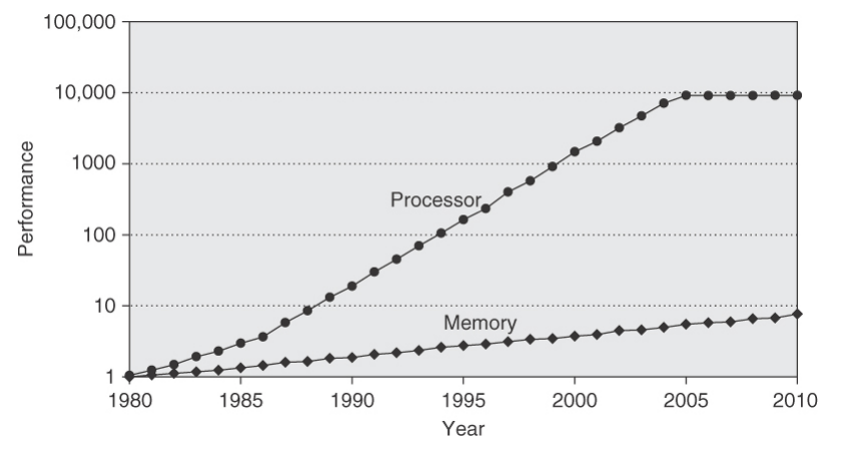
\includegraphics[width=0.7\linewidth]{fig/cpuvsmemory.jpg}
\caption{\it{The gap in performance, measured as the difference in the time 
between processor memory requests (for a single processor or core) and the 
latency of a DRAM access, is plotted over a $30$ year span~\cite{comparchbook}.}}
\label{fig:cpuvsmemory}
\end{figure}
%---------------------------
In multi-core systems, shared memory access conflicts between cores result in large access request queues. Figure~\ref{fig:multicore_arch}  illustrates a general multi-core architecture. The bank queues are served every memory clock cycle and the acknowledgement with data is sent back to the corresponding processor. In scenarios where multiple cores request access to memory locations in the same bank, the memory controller arbitrates them using bank queues. This contention between cores to access from the same bank is known as a {\em bank conflict}. As the number of bank conflicts increases, the resultant increases in memory access latency causes the multi-core system to slow.

%---------------------------
\begin{figure}[t!]
\centering
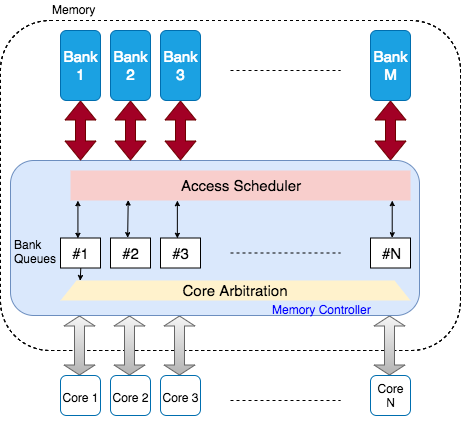
\includegraphics[width=\linewidth]{fig/fig-2-memory-controller.png}
\caption{\it{General multi-core architecture with a shared memory. $N$ processor cores share a memory consisting of $M$ banks.}}
\label{fig:multicore_arch}
\end{figure}
%---------------------------
We address the issue of increased latency by introducing a coded memory design. The main principle behind our memory design is to distribute accesses intended for a particular bank across multiple banks. We redundantly store encoded data, and we decode memory for highly requested memory banks using idle memory banks. This approach allows us to simultaneously serve multiple read requests intended for a particular bank. Figure~\ref{fig:example_xor} shows this with an example. Here, Bank 3 is redundant as its content is a function of the content stored on Banks 1 and 2. Such redundant banks are also referred to as {\em parity banks}. Assume that the information is arranged in $L$ rows in two first two banks, represented by $[a(1),\ldots, a(L)]$ and $[b(1),\ldots, b(L)]$, respectively. Let $+$ denote the XOR operation, and additionally assume that the memory controller is capable of performing simple decoding operations, \textit{i.e.} recovering $a(j)$ from $b(j)$ and $a(j) + b(j)$. Because the third bank stores $L$ rows containing $[a(1) + b(1),\ldots, a(L) + b(L)]$, this design allows us to simultaneously serve any two read requests in a single memory clock cycle.   

%---------------------------
\begin{figure}[t!]
\centering
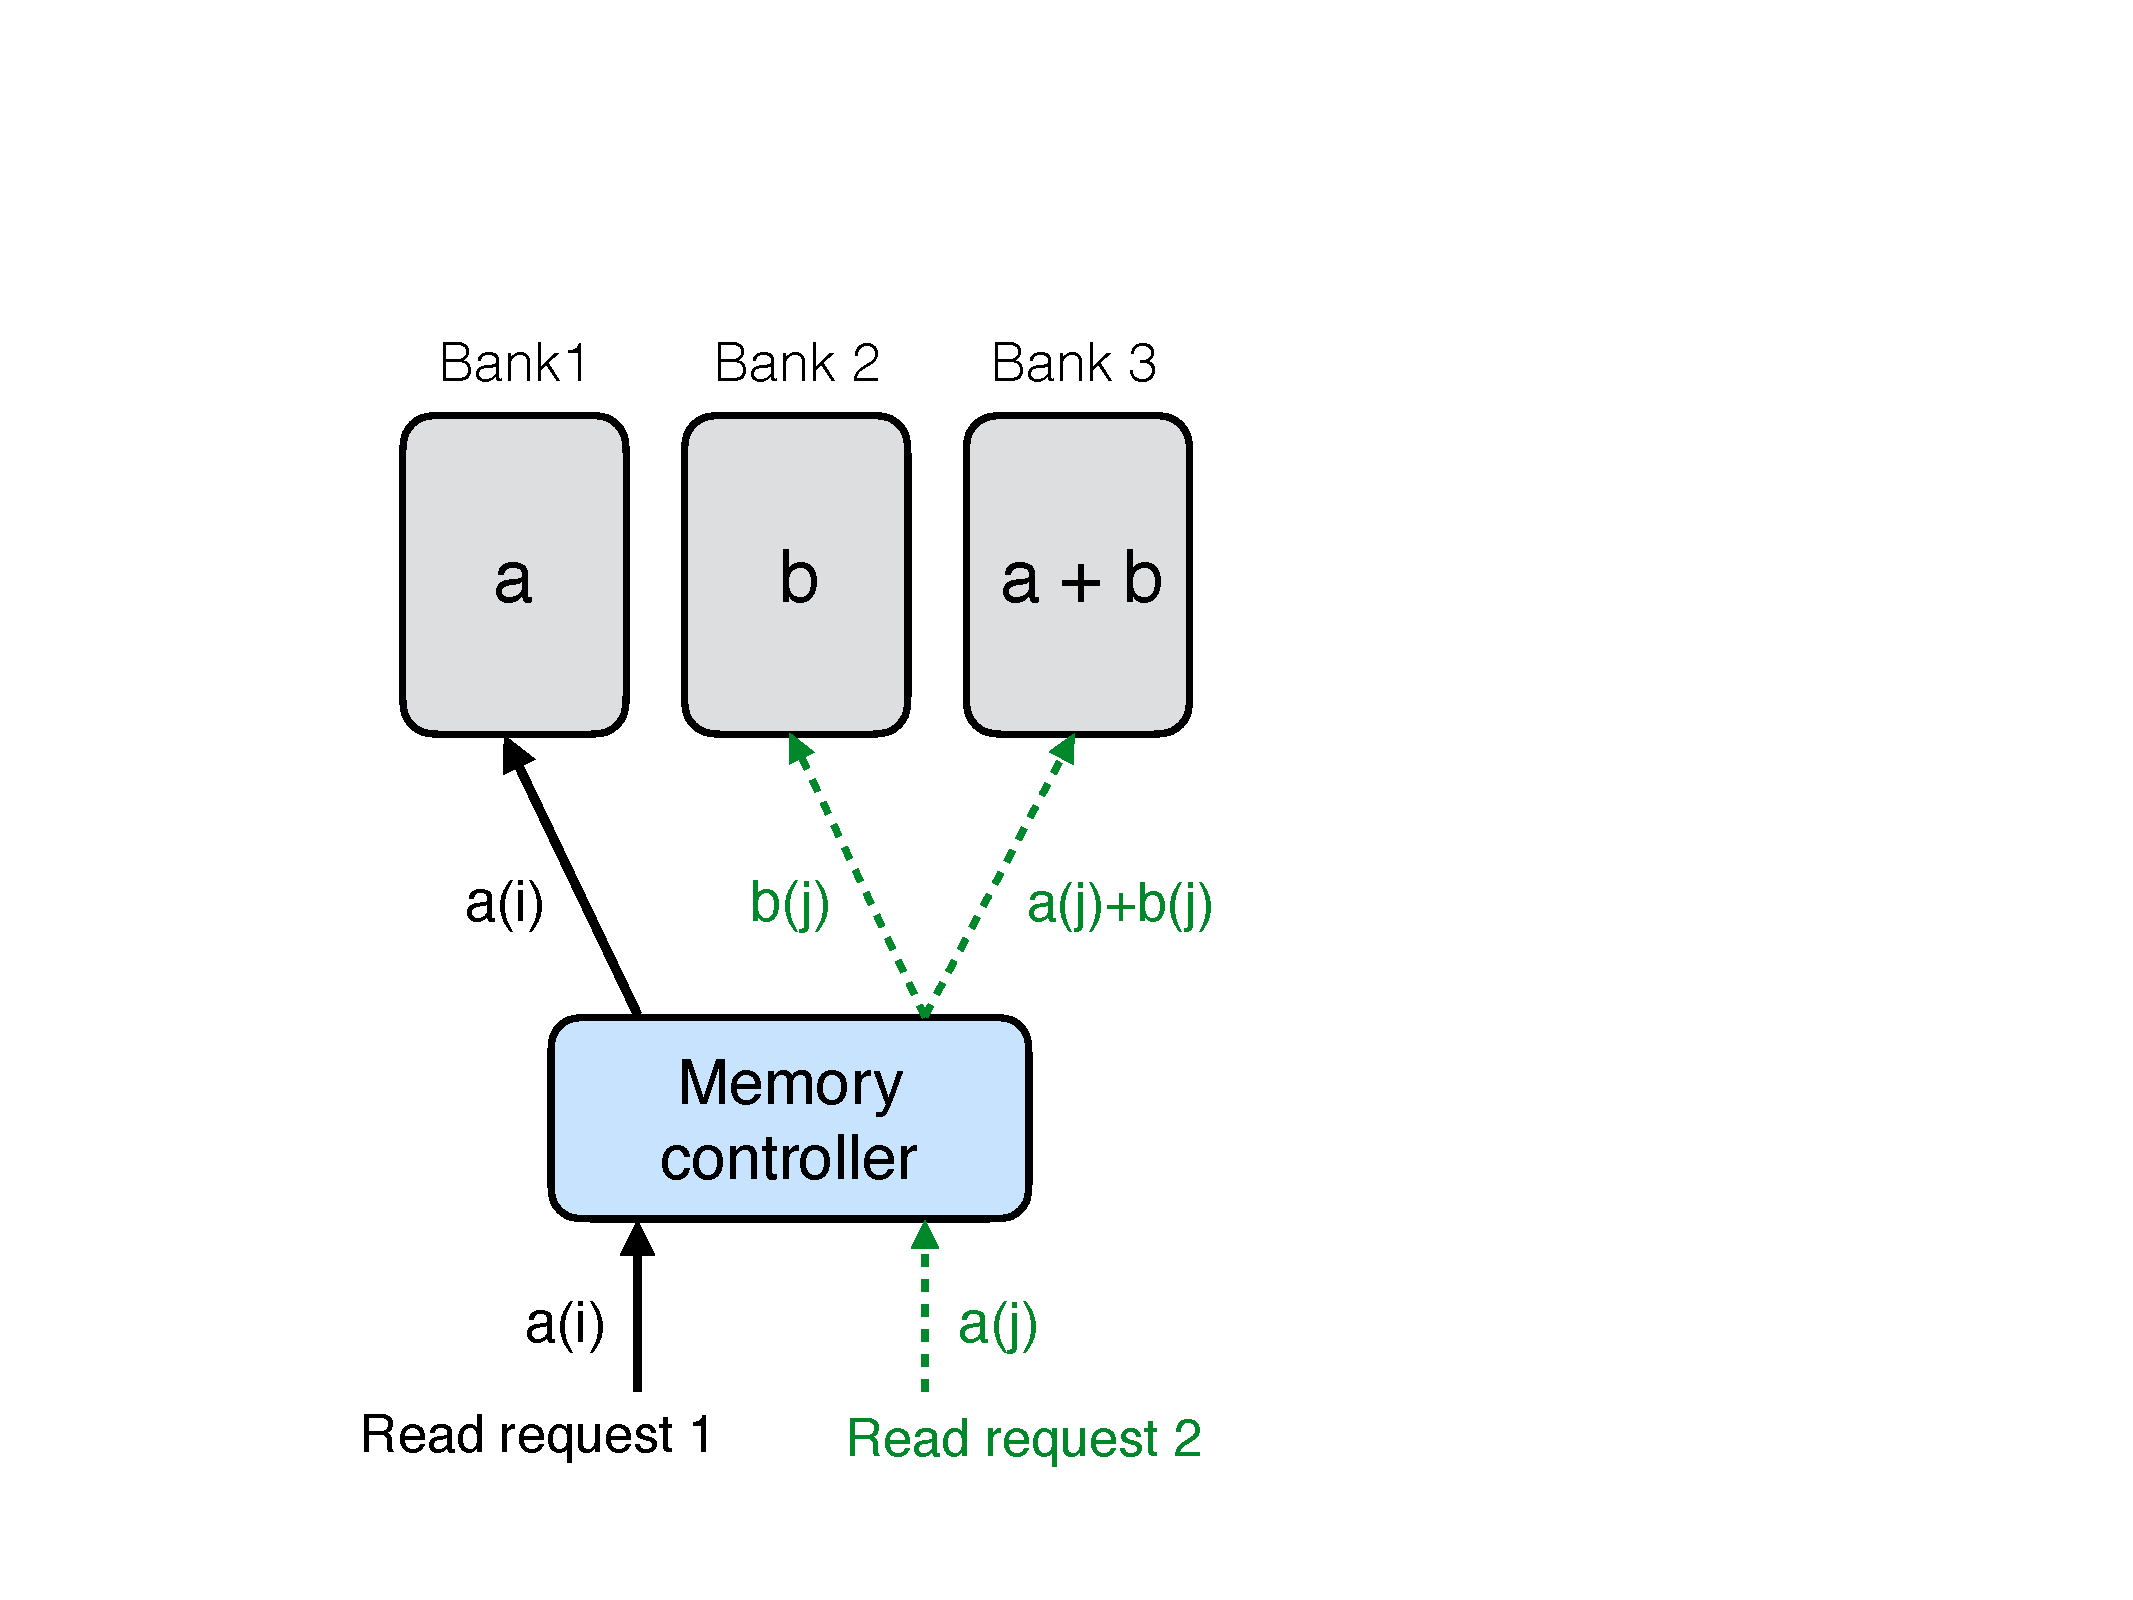
\includegraphics[width=0.395\linewidth]{fig/example-xor.pdf}
\caption{\it{Here the redundant memory in Bank 3 enables multiple read accesses to Bank 1 or 2. Given two read requests $\{a(i), a(j)\}$ directed to Bank $1$, we can deal with bank conflict in the following manner: 1) The first request for $a(i)$ is directly served by Bank $1$ itself.  2) The read request for $a(j)$ is served by downloading $b(j)$ and $a(j) + b(j)$ from Bank 2 and Bank 3, respectively. Another case where two read requests corresponding to two different banks, e.g., $\{a(i), b(j)\}$, can be simultaneously served from their respective banks without utilizing Bank $3$.}}
\label{fig:example_xor}
\end{figure}
%---------------------------
Hybrid memory designs such as the one in Figure~\ref{fig:example_xor} have additional requirements on top of serving read requests. The presence of redundant parity banks raises a number of challenges while serving write requests. The memory overhead of redundant memory storage adds to the overall cost of such systems, so efforts must be made to minimize this overhead. Finally, the heavy memory access request rate possible in multi-core scenarios necessitates sophisticated scheduling strategies to be performed by the memory controller. In this paper we address these design challenges and evaluate potential solutions in a simulated memory environment. 

\noindent \textbf{Main contributions and organization:~}In this paper we systematically address all key issues pertaining to a shared memory system that can simultaneously service multiple access requests in a multi-core setup. We present all the necessary background on realization of multi-port memories using single-port memory banks along with an account of relevant prior work in Section~\ref{sec:bg}. We then present the main contributions of the paper which we summarize below. %Here, we highlight the main contributions of the paper.
\begin{itemize}
\item We focus on the design of the storage space in Section~\ref{sec:code_design}. In particular, we employ three specific coding schemes to redundantly store the information in memory banks. These coding schemes, which are based on the literature on distributed storage systems~\cite{dimakis, Gopalan12, batchcodes, RPDV16}, allow us to realize the functionality of multi-port memories from single port memories while efficiently utilizing the storage space. Moreover, these coding schemes have low complexity encoding and decoding processes that require only simple XOR operations. %We focus on two specific memory designs that store information in memory banks based on two different coding schemes from the literature on distributed storage systems (a.k.a. cloud storage systems)~\cite{dimakis, Gopalan12, batchcodes, RPDV16}. These coding schemes allow us to realize the functionality of multi-port memories from a single port memories while efficiently utilizing the storage space. Moreover, these coding schemes have low complexity encoding and decoding processes that require only simple XOR operation.
\item We present a memory controller architecture for the proposed coding based memory system in Section~\ref{sec:memcontrol}. Among other issues, the memory controller design involves devising scheduling schemes for both read and write requests. This includes careful utilization of the redundancy present in the memory banks while maintaining the validity of information stored in them.
%In our setup, these scheduling schemes need to take the underlying coding scheme into account in order to utilize the redundancy present in the array of memory banks in the best possible manner. Furthermore, we also address the issue of keeping track of the validity of the information stored in various banks. Note that, due to unserved previous write requests, some of the stored data might have become outdate as far as a particular read request is concerned.
%able to serve the masecond main component of a shared memory system, i.e., memory controller, in Section~\ref{sec:memcontrol}. The memory controller design We also design the memory controllers for the proposed memory systems based on the storage pattern in different memory banks. Note that the memory controller design involves devising buffering and arbitration (scheduling) schemes for both read and write requests.
\item Focusing on applications where memory traces might exhibit favorable access patterns, we explore two ways to improve the efficiency of our coding based memory design in Sections~\ref{sec:dynamicCoding} and~\ref{sec:prefetching}. First, we propose a dynamic coding scheme which is based on detection of continuous heavily accessed regions of memory. 
%The dynamic coding scheme only encode these heavily access regions at a particular time instance. As different (uncoded) regions begin receiving more accesses, the dynamic coding scheme updates the content of parity (redundant) memory banks by encoding these regions. 
The second solution involves predicting the patterns of memory addresses over time. 
%Based on this prediction, the data from free bank is prefetched to serve subsequent request for information with the help of the prefetched data. This creates the opportunities to serve a large number of access requests in a given memory clock cycle. We note that the design of such prefacing schemes crucially depends on the underlying coding scheme.
%with Accompanied the design using dynamic coding where data is moved between coded and uncoded states. Utilized the coded memory system to perform useful data prefetching.
\item Finally, we conduct a detailed evaluation of the proposed designs of shared memory systems in Section~\ref{sec:experimentalmethodology}. We implement our memory designs by extending Ramulator, a DRAM simulator.~\cite{Ramulator}. We use the gem5 simulator~\cite{parsec_2_1_m5} to create memory traces of the PARSEC benchmarks~\cite{bienia09parsec2} which are input to our extended version of Ramulator. We then observe the execution-time speedups our memory designs yield.%a Implementation of the proposed solution using system C. Performance evaluation of the proposed solution on real memory traces with the help the system C implementation.  evaluate each
%of them for their cost. We also implement these designs using systemC and regress it throughmemory traces from real multi-core system.
\end{itemize}

%problem of concentrated accesses to a particular bank by normalizing it across 
%several banks. The solution is to use coding theory techniques to create 
%redundancy across banks, increasing the number of parallel accesses per cycle.  
%The queue build up on a bank is serviced through parallel access to several 
%additional banks, known as parity banks. The additional bank accesses results in 
%a decrease in number of contended memory accesses between cores, therefore 
%reducing the overall latency of the system. The reduction in the latency can be 
%seen directly as an increase in the overall system performance. 
%We present various design to store the redundancy across the parity banks and evaluate each
%of them for their cost. We also implement these designs using systemC and regress it through
%memory traces from real multi-core system.
%We show that 
%with a memory overhead of 15 $\%$; we can enable 4 extra read accesses / 2 extra 
%write accesses to a bank while remaining within the given design parameters. 

%{\color{blue}
%\subsection{Main contributions}
%
%Here, we summarize the main contributions of this paper. 
%\begin{itemize}
%\item Taking a coding theoretic approach to address the issue of realizing multi-port memories from single port memories. 
%\item Designed the memory controller accordingly:
%\begin{itemize}
%\item Involves devising scheduling schemes for both read and write requests.
%\end{itemize}
%\item Accompanied the design using dynamic coding where data is moved between coded and uncoded states. 
%\item Utilized the coded memory system to perform useful data prefetching.
%\item Implementation of the proposed solution using system C. Performance evaluation of the proposed solution on real memory traces with the help the system C implementation. 
%\end{itemize}
%}

%\noindent \textbf{Organization:~} The rest of the paper is organized as follows.

%\textbf{Key issues that need to be addressed}

%\begin{itemize}
%\item Design of storage space, i.e., how the data is distributed among different memory banks. This includes generation of redundancy (parity bits) based on the original data and allocation of these parity bits to the memory banks.
%\item Keeping track of the validity of the data stored in various banks. Note that, due to unserved previous write requests, some of the stored data might have become outdate as far as a particular read request is concerned.
%\item Resource allocation/arbitration among the different read and write requests originated from the same or different processors. The arbitration mechanism should take multiple criterion into account, including performance (i.e., the latency viewed by the processors), efficient utilization of the storage space (i.e., minimize the unused memory bank during a given period of time), and fairness (i.e., no processor should unnecessarily suffer due to requests from other processors getting prioritized).
%\end{itemize}

%%%%%%%%%%%%

%Coding theory is the study of codes and their applications to specific fields. Coding has been used in a variety of computer science applications, from error correcting in the transmitting of data to increased data storage compression. We aim to extend the benefits of coding theory to dynamic random-access memory systems. We propose a memory scheme in which a small portion of memory is reserved for the efficient coding of pre-existing data. In essence, this allows the data of one bank to be duplicated and stored in an additional memory location. Traditionally, when multiple requests to a single bank are issued by the processor, a stall is generated. These types of stalls, known as bank conflicts, result from the fact that only one address from a single bank can be accessed at a time. The processor must wait for the result from the first bank access to return before it can serve additional requests to the same bank. This lag can be a major bottleneck in a computer's processing speed. With a coded memory scheme, data present in multiple data banks will be compressed and stored in extra banks, known as a parity banks. These parity banks will then be accessed concurrently with corresponding data banks to help alleviate stalls from bank conflicts. Ultimately, with the addition of a single parity bank we are able to generate a single additional access to any arbitrary bank without implementing any further logic to the bank itself.
In the following sections, we first describe the design parameters used to design the coding system. We then describe the two coding designs we have implemented, and give the initial results we have achieved through the implementation of these designs. We also describe certain techniques to reduce the cost of coding implementation.



%In this section, we discuss various design parameters that we use in this phase of the project to design and simulate the efficient code storage. \\
\textit{Memory overhead}: The gains of multiple accesses to a memory bank every cycle comes with an associated cost. The cost is to store the compressed redundancy or the codes. The extra memory space used to store these codes is limited to 15$\%$ of the overall memory.\\
\textit{Memory size}: is an important parameter for consideration in design. The memory size and the parity storage size decide the code function to be used to essentially compress the redundant data. This design is considered for memory size of 8kB � 256 kB. This is the shared part of the memory which would be accessed by all the cores. \\ 
\textit{Memory Banks}: The memory banks essentially are the units which store the data. We consider the code design for 8 memory banks. We consider the memory banks addressed with Least Significant Bits (LSBs) of the address. The last 3 bits of the address decide which bank, the memory address belongs to and the rest of the MSBs decide the location within the bank.\\ 
\textit{Cache line size}: The memory accesses happen in burst as a cache line is evicted from the cache and is requested to be replaced by the cores. The cache controller thus requests a cache line which is a starting address and the length of the cache line. In this design, we consider cache line size of 128 bytes and 256 bytes. However, each core can potentially have a different cache line size and the concept of coding could be extended for various sizes.\\ 
\textit{Element size}:  Each memory location in a memory bank stores 256 bit of data. This essentially relates to decoding/understanding the address access request to the memory bank. The cores request memories to be read or written for multiple elements. For example, a core with 128 bytes of cache line would request 4 elements of read/write for each cache line. The shared traces have two different request patterns, for 128 bytes and for 256 bytes. \\
\textit{Number of Cores}: This parameter refers number of cores making access to the memory controller. This parameter is not used in the design of the coding scheme. However, we validate the design using the 6 core access trace shared with us for LTE and UMTS. \\
\textit{Access rate}: This is the average rate at which the memory controller executes the reads/writes to the memory banks. In this design, we consider 1.54 ns as the access rate. This would mean that the clock rate to memory would be at 650MHz. This parameter is required to simulate the performance for the shared traces. 


\section{Codes to Improve Accesses}
\label{sec:code_design}

%In this section, we discuss one of the main components of the memory design proposed in this paper. 
Introducing redundancy into a storage space comprised of single-port memory banks enables simultaneous memory access. In this section we propose memory designs that utilize coding schemes which are designed for access-efficiency. We first define some basic concepts with an illustrative example and then describe $3$ coding schemes in detail.

\begin{comment}
Coding theory is the study of codes and their applications  to specific fields.  
Coding has been used in a variety of computer  science applications,  from error 
correction in the transmission of data  to increased compression for data  
storage.  We aim to extend the benefits of coding theory  to improve the 
efficiency of random-access  memory systems.  We propose a memory scheme in 
which a small portion of memory is reserved for the efficient coding of 
pre-existing data.  In essence, this allows the data of one bank to be 
duplicated and stored in an additional memory location.  Traditionally, when 
multiple  requests  to a single bank  are issued by the processor, a stall is 
generated.  These types of stalls, known as bank conflicts, result from the fact 
that  only one address from a single bank can be accessed at a time.  The 
processor must wait for the result from the first bank access to return  before 
it can serve additional  requests to the same bank.  This lag can be a major 
bottleneck in a computer's processing speed. With a coded memory scheme, data 
present in multiple data banks will be compressed and stored in extra banks, 
known as a parity banks.  These parity banks will then be accessed concurrently 
with corresponding data  banks to help alleviate stalls from bank conflicts.  
Ultimately,  with the addition  of a single parity  bank we are able to generate 
a single additional  access to any arbitrary bank  without  implementing  any 
further  logic to the bank  itself.  In the following sections, we first 
describe the design parameters used to design the coding system.  We then 
describe each of the three code schemes explored in this project.
\end{comment}

\subsection{Coding for memory banks}
\label{sec:coding_mb}

A coding scheme defines how memory is encoded to yield redundant storage. The memory structures which store the original memory elements are known as {\em data banks}. The elements of the data banks go through an {\em encoding process} which generates a number of {\em parity banks}.  The parity banks contain elements constructed from elements drawn from two or more data banks. A linear encoding process such as XOR may be used to minimize computational complexity. The following example further clarifies these concepts and provides some necessary notation.

\begin{example}
Consider a setup with two data banks $\mathbf{a}$ and $\mathbf{b}$. We assume that each of the banks store $L \cdot W$ binary data elements\footnote{It is possible to work with data elements over larger alphabets/finite fields. However, assuming data elements to be binary suffices for this paper as only work with coding schemes defined over binary field.} which are arranged in an $L \times W$ array. In particular, for $i \in [L] \triangleq \{1,\ldots, L\}$, $a(i)$ and $b(i)$ denote the $i$-th row of the bank $\mathbf{a}$ and bank $\mathbf{b}$, respectively. Moreover, for $i \in [L]$ and $j \in [W] \triangleq \{1,\ldots, W\}$, we use $a_{i, j}$ and $b_{i, j}$ to denote the $j$-th element in the rows $a(i)$ and $b(i)$, respectively. Therefore, for $i \in [L]$, we have 
\begin{align}
a(i) = \big(a_{i,1}, a_{i,2},\ldots, a_{i, W}\big) \in \{0, 1\}^W\nonumber \\
b(i) = \big(b_{i,1}, b_{i,2},\ldots, b_{i, W}\big) \in \{0, 1\}^W. \nonumber
\end{align}
Now, consider a linear coding scheme that produces a parity bank $\mathbf{p}$ with $L'W$ bits arranged in an $L' \times W$ array such that for $i \in [L'] \triangleq \{1,\ldots, L'\}$, 
\begin{align}
p(i) &= \big(p_{i, 1},\ldots, p_{i,W}\big) = a(i) + b(i) \nonumber \\
&\triangleq \left(a_{i,1} + b_{i,1}, a_{i,1} + b_{i,1},\ldots, a_{i,1} + b_{i,1}\right). 
\end{align}
\end{example}
\begin{remark}
Figure~\ref{fig:example1} illustrates this coding scheme. Because the parity bank is based on those rows of the data banks that are indexed by the set $[L'] \subseteq [L]$, we use the following concise notation to represent the encoding of the parity bank. 
$$
\mathbf{p} = \mathbf{a}([L']) +  \mathbf{b}([L']).
$$
In general, we can use any subset $\mathcal{S} = \{i_1, i_2,\ldots, i_{L'}\} \subseteq [L]$ comprising $L'$ rows of data banks to generate the parity bank $\mathbf{p}$. In this case, we have $\mathbf{p} = \mathbf{a}(\mathcal{S}) +  \mathbf{b}(\mathcal{S})$, or
\begin{align*}
p(l) = a(i_l) + b(i_l)~\text{for}~l \in [L'].
\end{align*}
%Figure~\ref{fig:example1_case2} illustrates the case with a generic set $\mathcal{S}$.% $ = [L - L'  + 1,\ldots, L]$.
\end{remark}

%%%%%%%%%%%%%%%%%%%%%%%%%%%%%%%%%%%
%\begin{figure}[t!]
%\centering
%\begin{subfigure}[b]{0.48\linewidth}
%  \centering
%  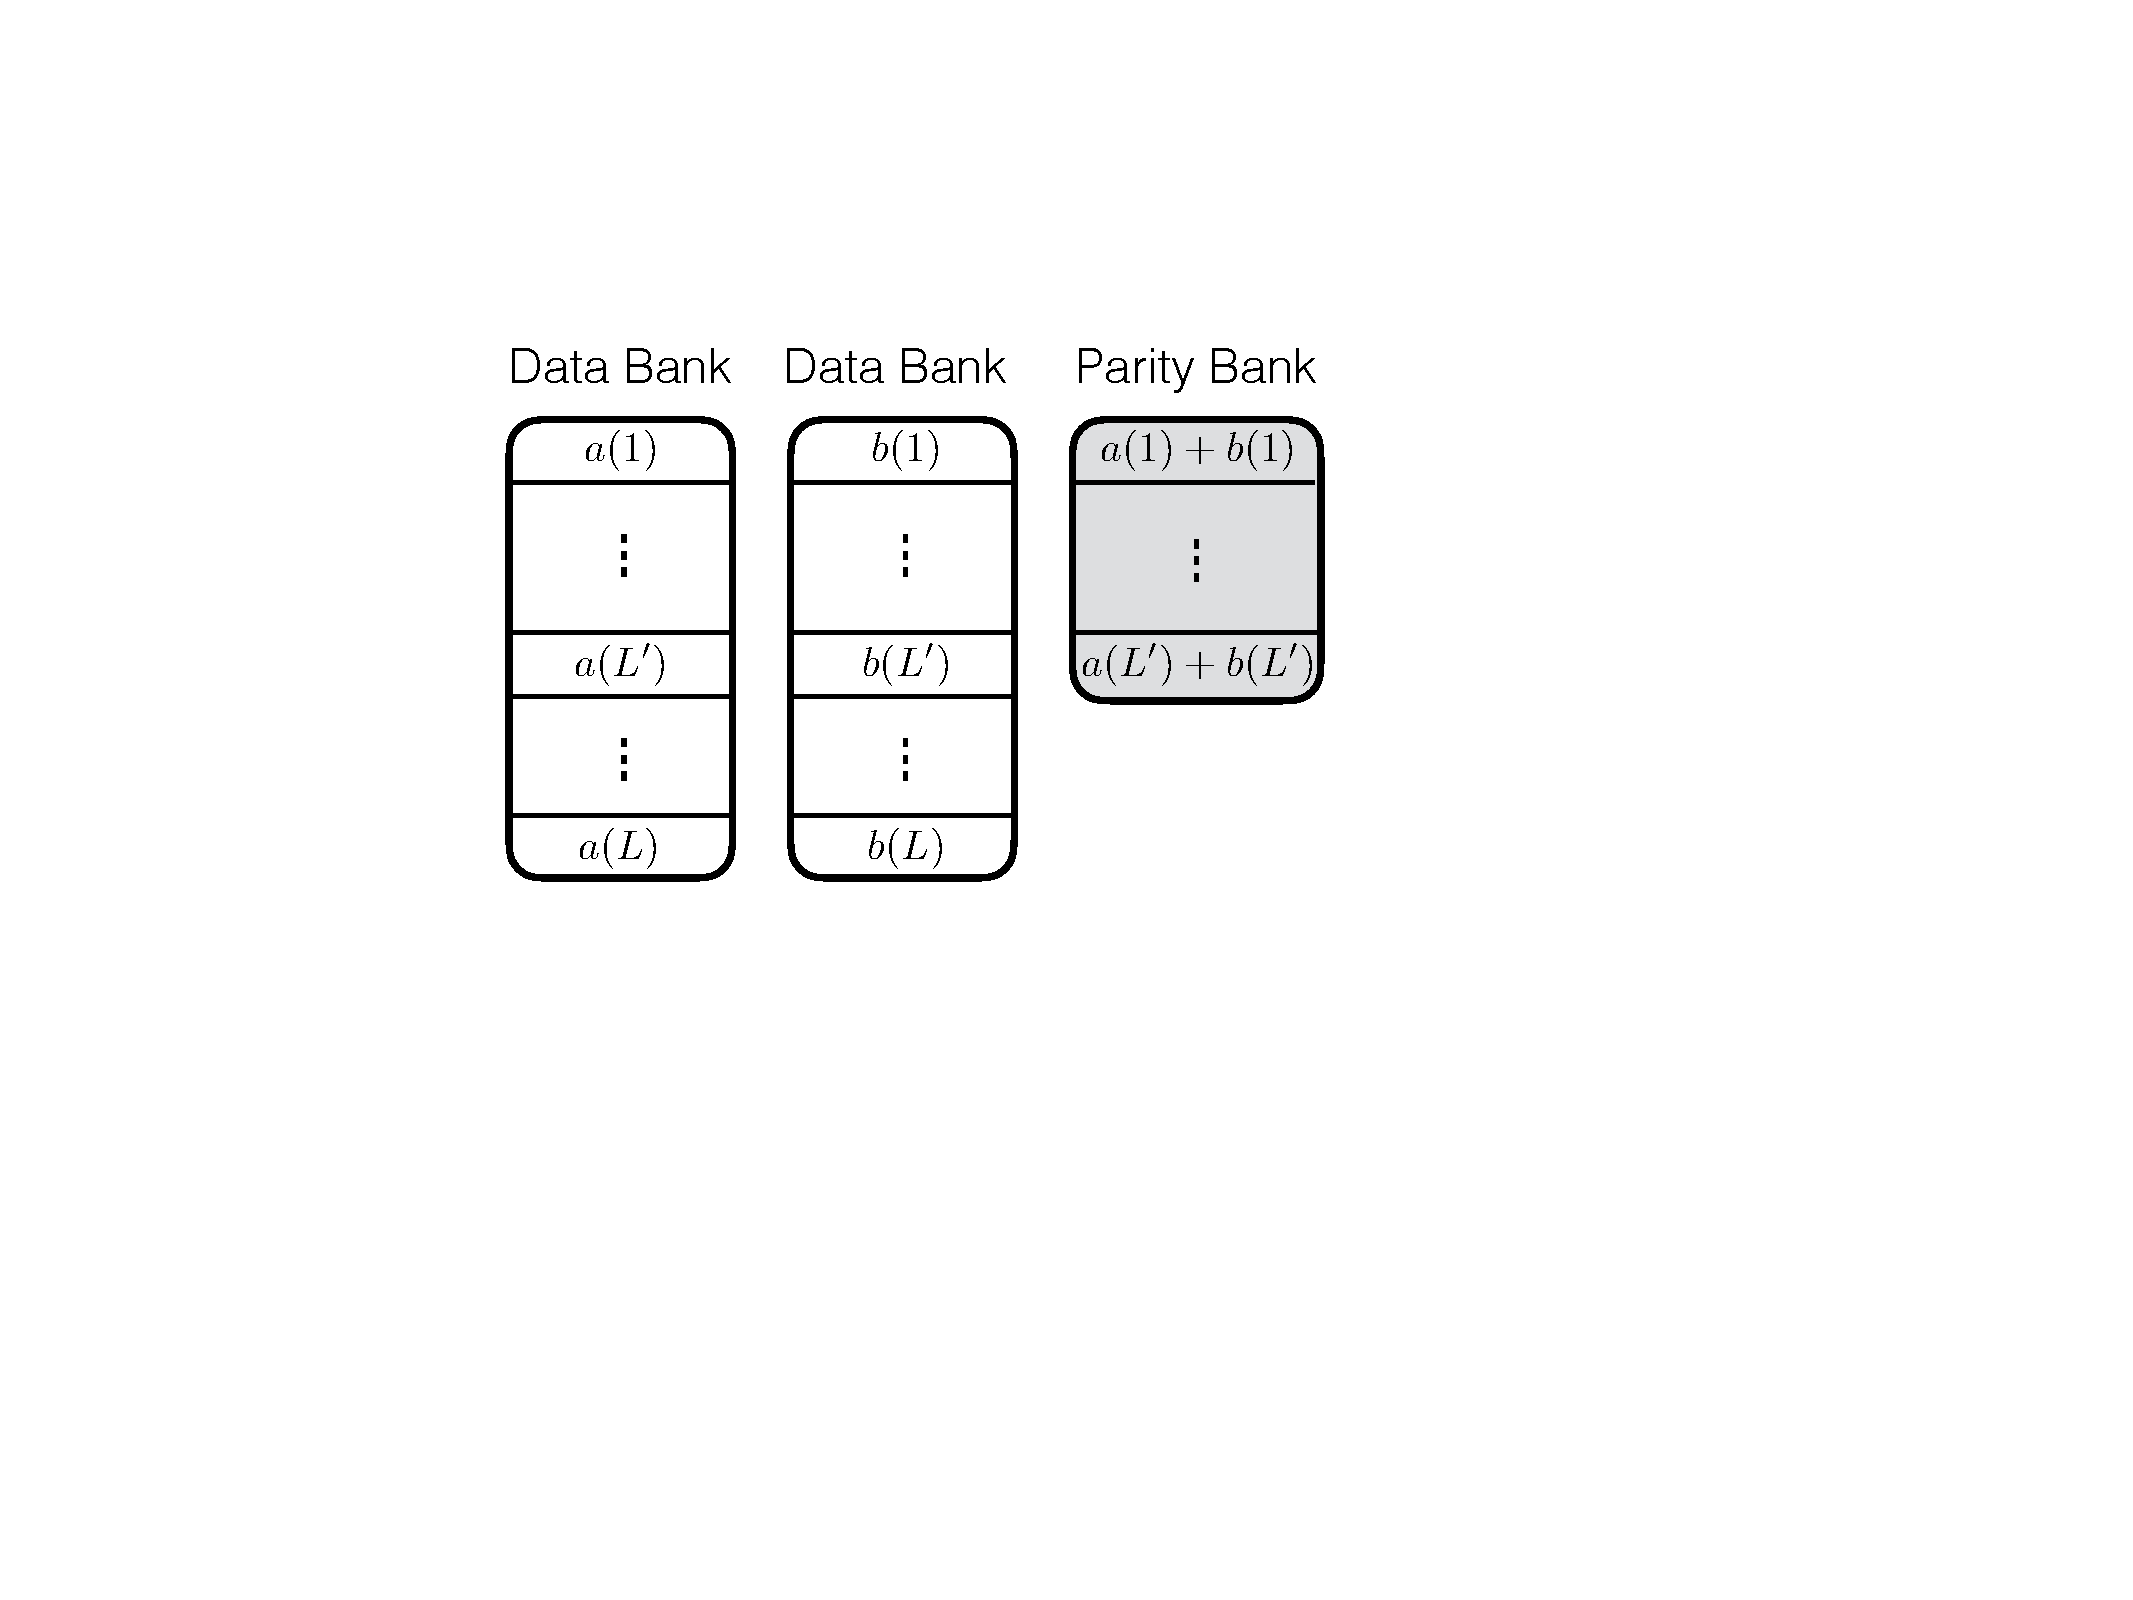
\includegraphics[width=0.95\linewidth]{fig/example-inter-bank.pdf} 
%  \caption{{\color{red}Parity.}}
%  \label{fig:example1_case1}
%\end{subfigure}
%\begin{subfigure}[b]{0.48\linewidth}
%  \centering
%  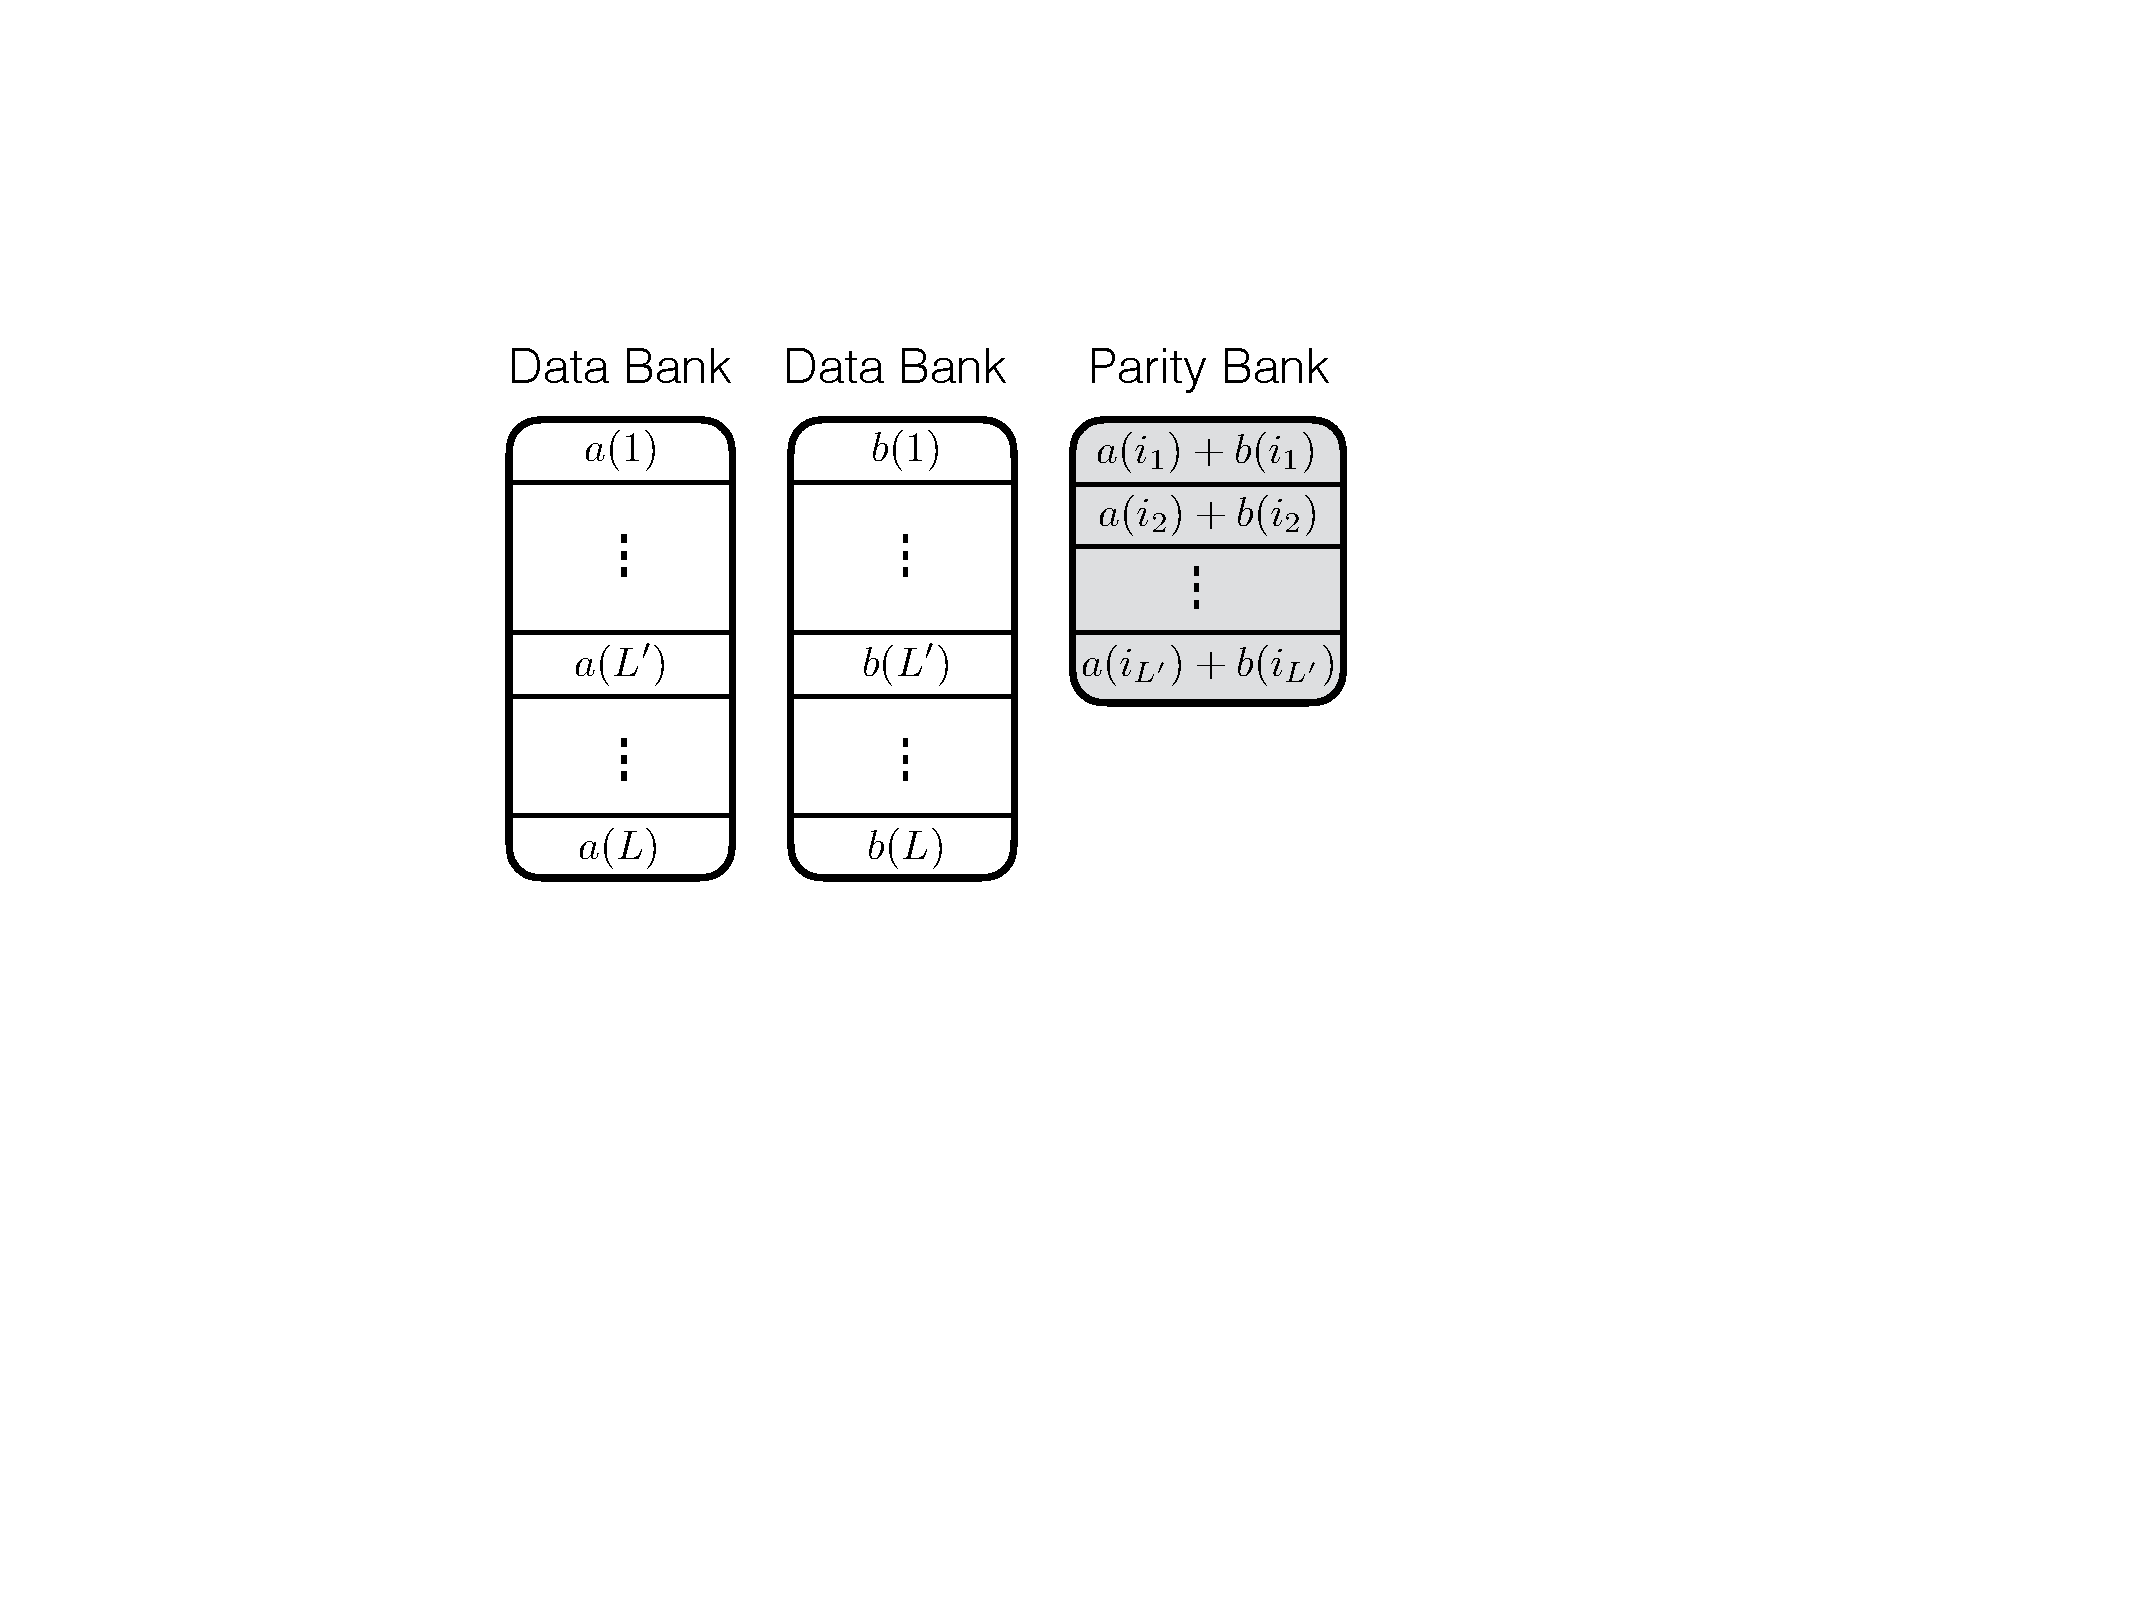
\includegraphics[width=0.98\linewidth]{fig/example-inter-bank-2.pdf} 
%  \caption{{\color{red}Parity.}}
%  \label{fig:example1_case2}
%\end{subfigure}
%\caption{{\color{red}Design.}}
%\label{fig:example1}
%\end{figure}
\begin{figure}[t!]
\centering
  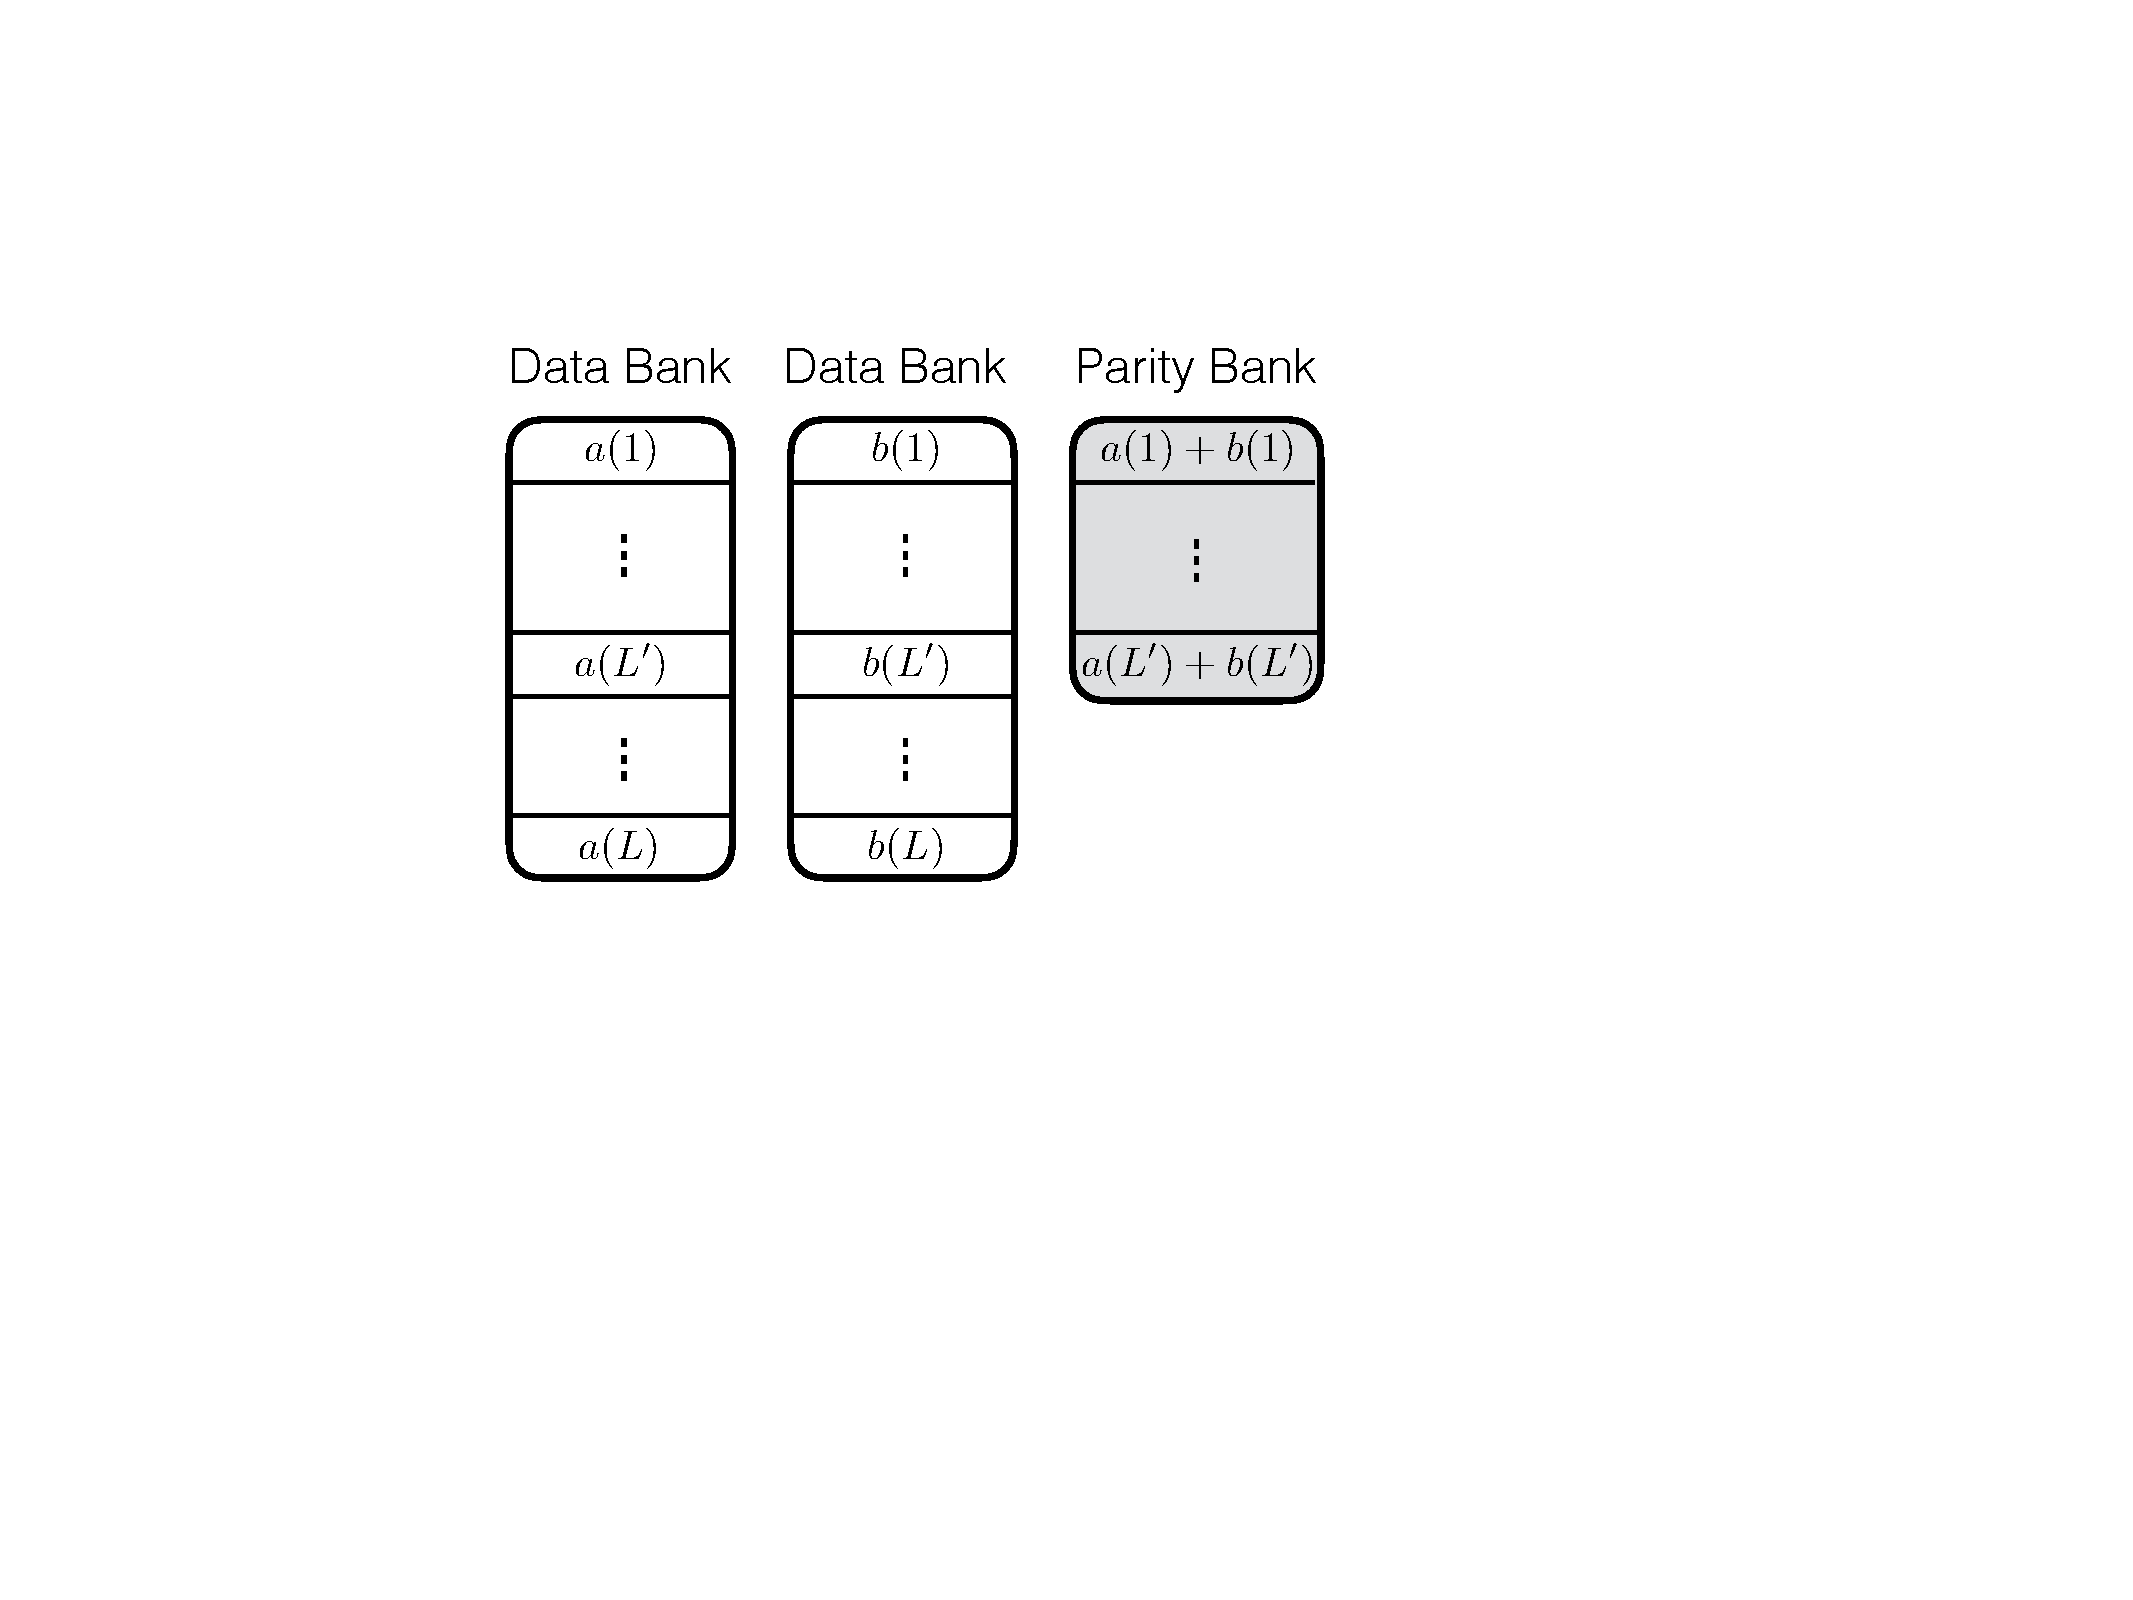
\includegraphics[width=0.45\linewidth]{fig/example-inter-bank.pdf} 
\caption{\it{This illustration is an example parity design.}}
\label{fig:example1}
\end{figure}
%%%%%%%%%%%%%%%%%%%%%%%%%%%%%%%%%%%%%%


\begin{remark}
Note that we allow for the data banks and parity banks to have different sizes, \textit{i.e.} $L \neq L'$. This freedom in memory design can be utilized to reduce the storage overhead of parity banks based on the underlying application. If the size of a parity bank is smaller than a data bank, \textit{i.e.} $L' < L$, we say that the parity bank is a {\em shallow bank}. We note that it is reasonable to assume the existence of shallow banks, especially in proprietary designs of integrated memories in a system on a chip (SoC).
\end{remark}

\begin{remark}
\label{rem:design1}
Note that the size of shallow banks is a design choice which is controlled by the parameter $0 < \alpha \leq 1$. A small value of $\alpha$ corresponds to small storage overhead. The choice of a small $\alpha$ comes at the cost of limiting parity memory accesses to certain memory ranges. In Section~\ref{sec:dynamicCoding} we discuss techniques for choosing which regions of memory to encode. In scenarios where many memory accesses are localized to small regions of memory, shallow banks can support many parallel memory accesses for little storage overhead. For applications where memory access patterns are less concentrated, the robustness of the parity banks allows one to employ a design with $\alpha = 1$.
\end{remark}

\subsubsection{Degraded reads and their locality}
\label{sec:degraded}

The redundant data generated by a coding scheme mitigates bank conflicts by supporting multiple read accesses to the original data elements. Consider the coding scheme illustrated in Figure~\ref{fig:example1} with a parity bank $\mathbf{p} = \mathbf{a}([L']) + \mathbf{b}([L'])$. In an uncoded memory system simultaneous read requests for bank $\mathbf{a}$, such as $a(1)$ and $a(5)$, result in a bank conflict. The introduction of $\mathbf{p}$ allows both read requests to be served. First, $a(1)$ is served directly from bank  $\mathbf{a}$. Next, $b(5)$ and $p(5)$ are downloaded. $a(5) = b(5) + p(5)$, so $a(5)$ is recovered by means of the memory in the parity bank. A read request which is served with the help of parity banks is called a {\em degraded read}. Each degraded read has a parameter {\em locality} associated with it which corresponds to the total number of banks used to serve it. In this case, the degraded read for $a(5)$ using $\mathbf{b}$ and $\mathbf{p}$ has locality $2$.

%In order to further illustrate the notion of locality, let's consider a setup where we generate a parity bank $\mathbf{p}$ by combining three data banks $\mathbf{a}$, $\mathbf{b}$, and $\mathbf{c}$ as $\mathbf{p} = \mathbf{a} + \mathbf{b} + \mathbf{c}$. Now, a degraded read for $a(1)$ using the parity bank as $$a(1) = b(1) + c(1) + p(1) = b(1) + c(1) + \big(a(1) + b(1) + c(1)\big)$$
%has locality $3$ as the degraded read is served using three memory banks.

\subsection{Codes to emulate multi-port memory}
\label{sec:designs}

We will now describe the code schemes proposed for the emulation of multi-port memories. Among a large set of possible coding schemes, we focus on three specific coding schemes for this task. We believe that these three coding schemes strike a good balance among various quantitative parameters, including storage overhead, number of simultaneous read requests supported by the array of banks, and the locality associated with various degraded reads. Furthermore, these coding schemes respect the practical constraint of encoding across a small number of data banks. In particular, we focus on the setup with $8$ memory banks, which contrasts with communications applications where encoding typically occurs with blocks of $1024$ or more information symbols. 

In the rest of this section, we present three code schemes and discuss the number of simultaneous read requests supported by these schemes in the best and worst case. We summarize all the relevant parameters associated with these schemes in Table~\ref{table:codedesigncomparison}.
%
%We discuss the design of the codes for creating extra accesses to memory in this 
%section. First we discuss the code schemes explored during Phase I. Second, we discuss 
%specific execution strategies to efficiently implement the designs.\\
%In the following sub-sections, we discuss 3 designs for storing coded data.  
%Table~\ref{table:codedesigncomparison} compares these designs for various 
%parameters and associated costs.  
%\begin{table*}[t]
%\centering
%	\begin{tabular}{|m{1cm}|m{2 cm}|m{1cm}|m{1cm}|m{1cm}|m{1cm}|m{1cm}|}
%\hline
%Design & Max Read per bank & Max Write per bank & Locality & Rate & Memory 
%Overhead & Logical Complexity \\ \hline
%I & 4 & 2 & 2 & $2/5$ & 1.5 $\alpha$ & Low \\ \hline
%II & 5 & 2 & 2 & $2/5$ & 2.5 $\alpha$ & Medium \\ \hline
%III & 4 & 2 & 3 & $1/2$ & \text{      } $\alpha$ & Medium \\ \hline
%	\end{tabular}
%	\caption{Comparison of design with respect to the performance parameters 
%	and associated cost}
%	\label{table:codedesigncomparison}
%\end{table*}


%\begin{tiny}
%\begin{table}[t!]
%  \centering
%  \begin{tabular}{|c|c|c|c|c|c|c|}
%    \hline
%    \textbf{Design} & \textbf{Max reads} & \textbf{Max writes} & \textbf{Locality} & \textbf{Rate} & \textbf{Storage overhead} & \textbf{Logical complexity} \\
%    & \textbf{(per bank)} & \textbf{(per bank)} & & & & \\
%    \hline
%    \hline
%    I & 4 & 2 & 2 & $2/5$ & 1.5 $\alpha$ & Low \\ \hline
%II & 5 & 2 & 2 & $2/5$ & 2.5 $\alpha$ & Medium \\ \hline
%III & 4 & 2 & 3 & $1/2$ & \text{      } $\alpha$ & Medium \\ 
%\hline                                   
%  \end{tabular}
%	\caption{Comparison of the code schemes with respect to the performance parameters and associated cost}
%	\label{table:codedesigncomparison}
%\end{table}
%\end{tiny}

\begin{comment}
\begin{table}[t!]
  \centering
  \begin{tabular}{|c|c|c|c|c|c|}
    \hline
   {\small Design} & {\small  Max reads} &{\small  Locality} & {\small  Rate} & {\small  Storage} & {\small  Logical } \\
    & {\small  (per bank)} & & &{\small  overhead} & {\small  complexity} \\
    \hline
    \hline
    {\small I} & {\small$4$ } & {\small$2$} & {\small ${2}/{5}$} & {\small $1.5\alpha$} & {\small Low} \\ \hline
{\small II} & {\small$5$}  & {\small$2$} & {\small ${2}/{5}$} & {\small $2.5\alpha$} & {\small Medium} \\ \hline
{\small III }& {\small$4$}  & {\small$3$} & {\small$1/2$} & {\small $\alpha$} & {\small Medium} \\ 
\hline                                   
  \end{tabular}
	\caption{\it{Comparison of the code schemes with respect to the performance parameters and associated cost. $\alpha$ is the fraction of storage overhead in comparison to the data bank. $\alpha = 1$ when size of parity bank is equal to size of data bank.}}
	\label{table:codedesigncomparison}
\end{table}
\end{comment}

\begin{table}[ht!]
  \centering
  \begin{tabular}{|c|c|c|c|c|c|}
    \hline
   {\scriptsize Design} & {\scriptsize  Max reads} &{\scriptsize  Locality} & {\scriptsize  Rate} & {\scriptsize  Storage} & {\scriptsize  Logical } \\
    & {\scriptsize  (per bank)} & & {\scriptsize ($\alpha=1$)}&{\scriptsize  overhead} & {\scriptsize  complexity} \\
    \hline
    \hline
    {\scriptsize I} & {\scriptsize$4$} & {\scriptsize$2$} & {\scriptsize $\nicefrac{2}{5}$} & {\scriptsize $1.5\alpha$} & {\scriptsize Low} \\ \hline
%{\scriptsize II} & {\scriptsize$5$}  & {\scriptsize$2$} & {\scriptsize ${2}/{5}$} & {\scriptsize $2.5\alpha$} & {\scriptsize Medium} \\ \hline
{\scriptsize II} & {\scriptsize$5$}  & {\scriptsize$2$} & {\scriptsize $\nicefrac{2}{7}$} & {\scriptsize $2.5\alpha$} & {\scriptsize Medium} \\ \hline
{\scriptsize III }& {\scriptsize$4$}  & {\scriptsize$3$} & {\scriptsize$\nicefrac{1}{2}$} & {\scriptsize $\alpha$} & {\scriptsize Medium} \\ 
\hline                                   
  \end{tabular}
	\caption{\it{Comparison of the code schemes with respect to the performance parameters and associated cost.}}
	\label{table:codedesigncomparison}
\end{table}


\subsubsection{Code Scheme I}
\label{sec:design1}

This code scheme is motivated from the concept of batch codes~\cite{batchcodes} which enables parallel access to content stored in a large scale distributed storage system.
%The coding scheme is illustrated in Figure~\ref{fig:design1}. 
The code scheme involves $8$ data banks $\{\mathbf{a}, \mathbf{b},\ldots, \mathbf{h}\}$ each of size $L$ and $12$ shallow banks each of size $L' = \alpha L$. We partition the $8$ data banks into two  groups of $4$ banks. The underlying coding scheme produces shallow parity banks by separately encoding data banks from the two groups. Figure~\ref{fig:design1} shows the resulting memory banks. The storage overhead of this schemes is $12\alpha L$ which implies the rate\footnote{The information rate is a standard measure of redundancy of a coding scheme ranging from $0$ to $1$, where $1$ corresponds to the most efficient utilization of storage space.} of the coding scheme is $$\frac{8L}{8L + 12\alpha L} = \frac{2}{2 + 3\alpha}.$$


We now analyze the number of simultaneous read requests that can be supported by this code scheme. \\
%This allows us to serve multiple accesses to the coded 
%region using the parity banks. With this scheme, we guarantee that any 4 read 
%requests to the coded region can be served at any given time. As shown in 
%figure~\ref{fig:design1}, 8 banks are divided into two regions.  Each region 
%consists of 4 banks. Each region has 6 parallel shallow  banks to store the 
%parity. The colored regions shown in the banks 1-8 are the coded region. These 
%regions are assumed to be of $\alpha $ fraction of the memory. \\

\noindent \textbf{Best case analysis:~}This code scheme achieves maximum 
performance when sequential accesses to the coded regions are issued. During the 
best case access, we can achieve up to $10$ parallel accesses to a particular coded region in one access cycle.
Consider the scenario when we receive accesses to the following $10$ rows:
\begin{align*}
&\left\{a(1),b(1),c(1),d(1),a(2),b(2),c(2),d(2),c(3),d(3)\right\} .
\end{align*}
Note that we can serve the read requests for the rows \\ $\{a(1),b(1),c(1),d(1)\}$ using the data bank $\mathbf{a}$ and the three parity banks storing $\{a(1)+b(1), b(1)+c(1),c(1)+d(1)\}$. The requests for $\{a(2),c(2),d(2)\}$ can be served by downloading $b(2)$ from the data bank $\mathbf{b}$ and $\{a(2)+d(2), b(2)+d(2),a(2)+c(2)\}$ from their respective parity banks. Lastly, in the same memory clock cycle, we can serve the requests for $\{c(3), d(3)\}$ using the data banks $\mathbf{c}$ and $\mathbf{d}$.\\
%------------------------------
\begin{figure}[ht!]
\centering
	%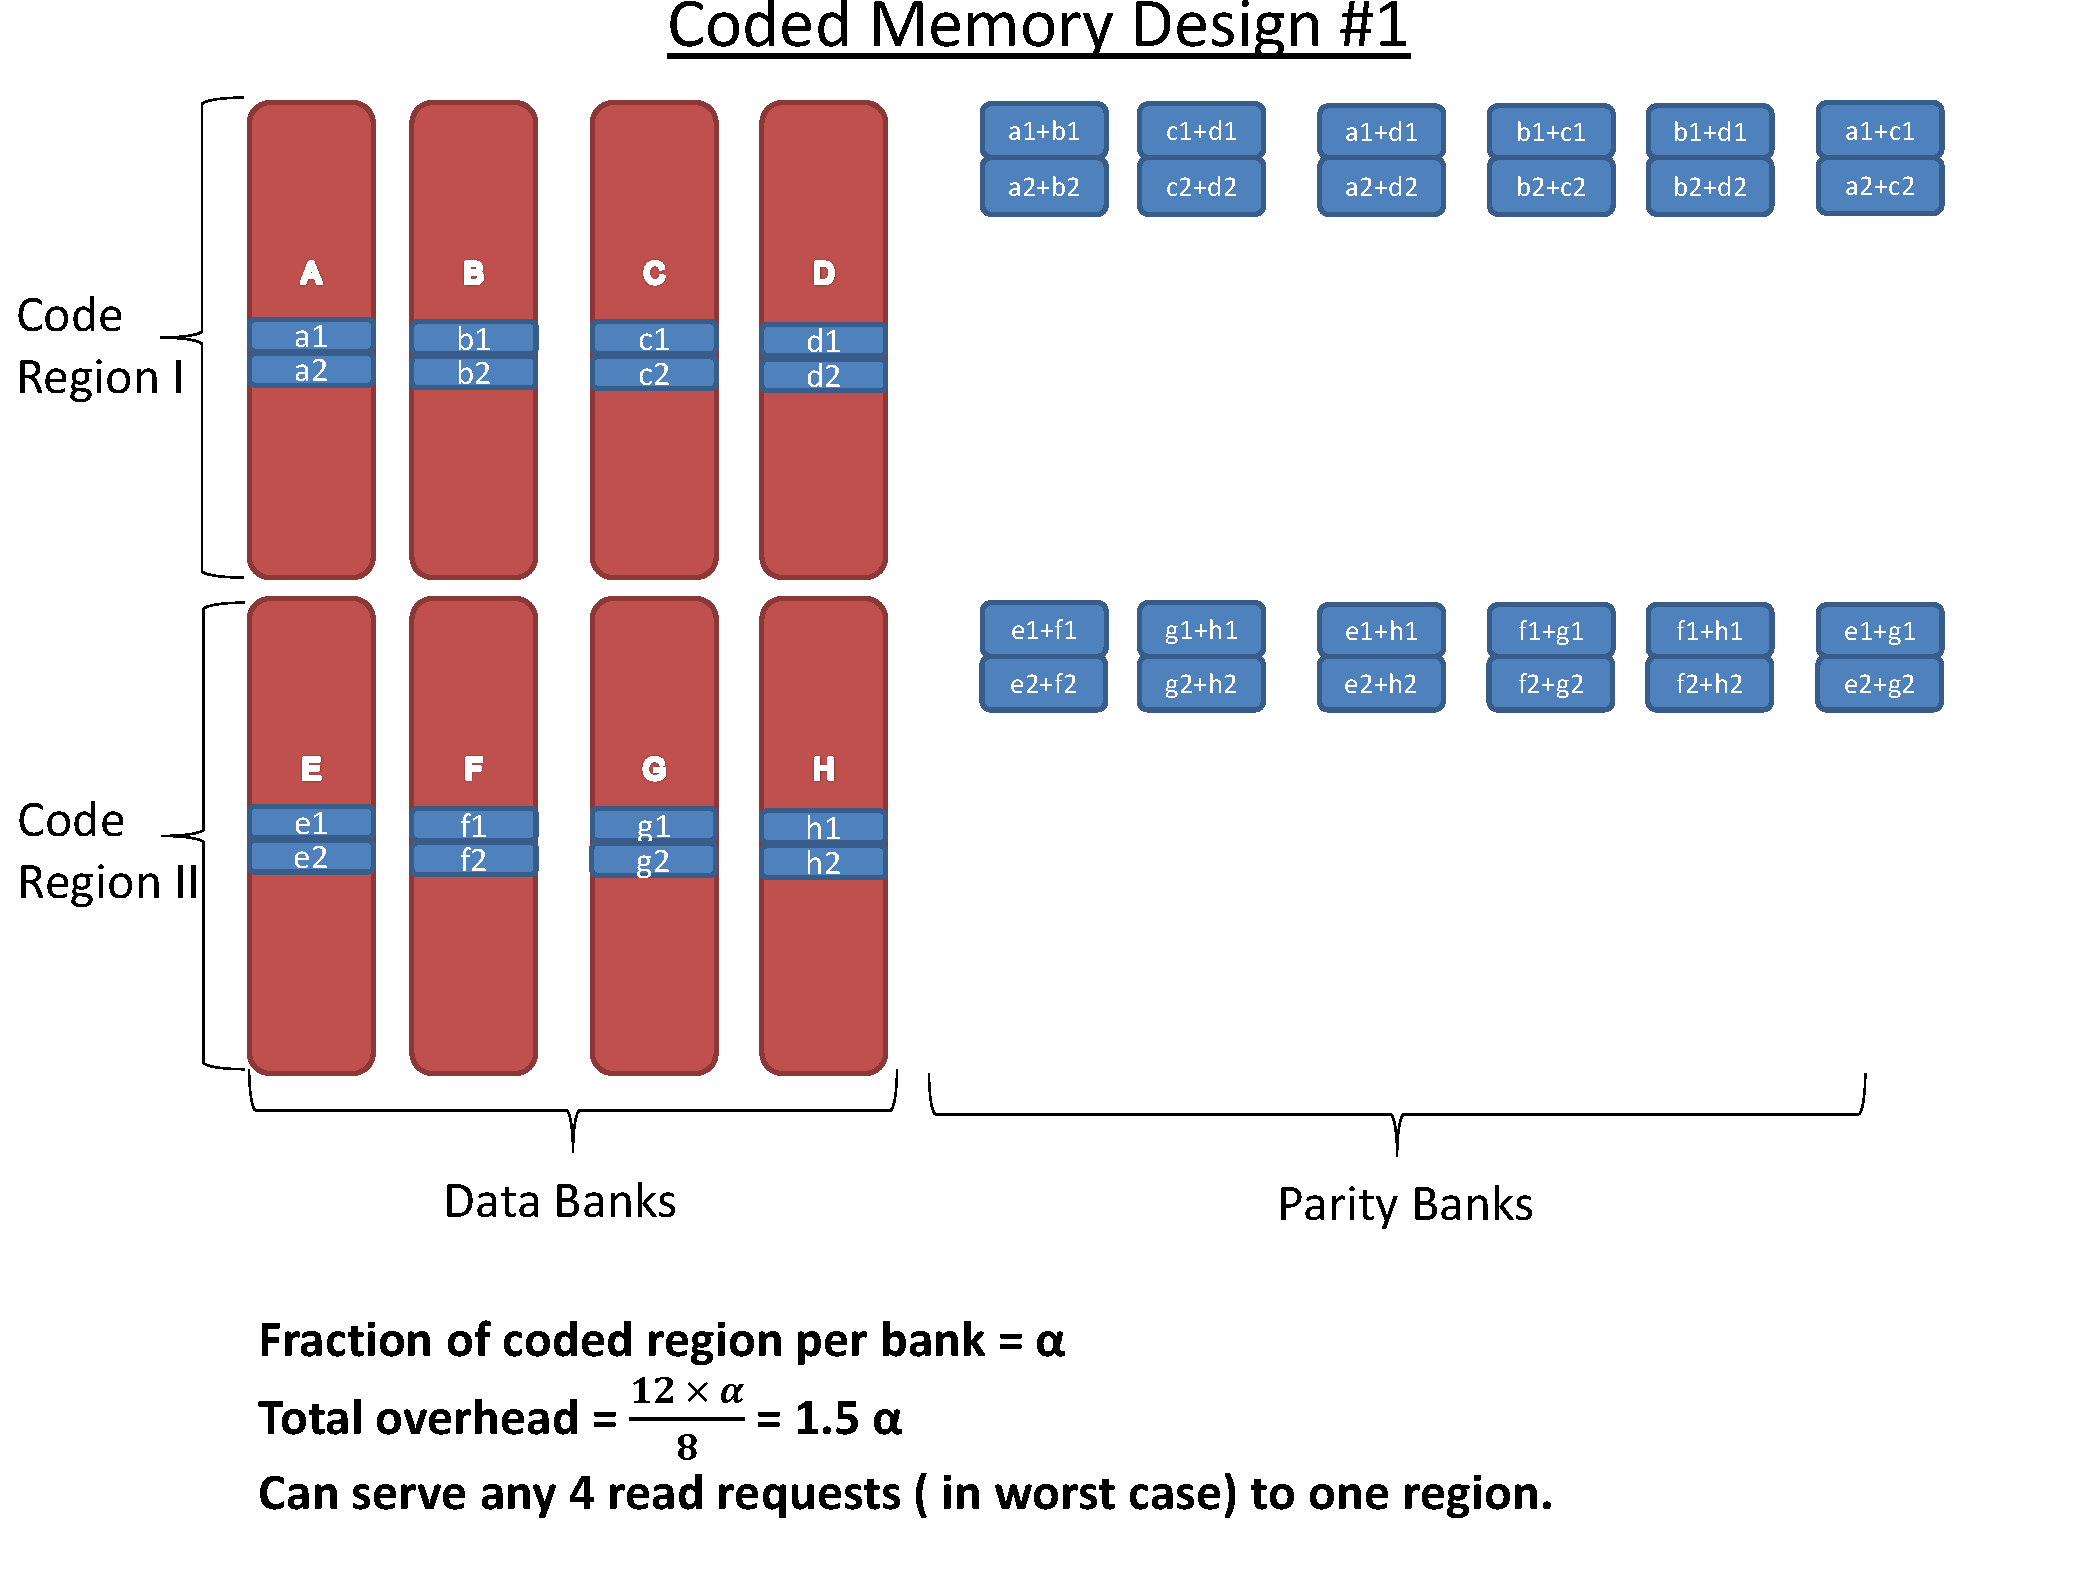
\includegraphics[width=0.8\linewidth]{fig/designI.pdf}
	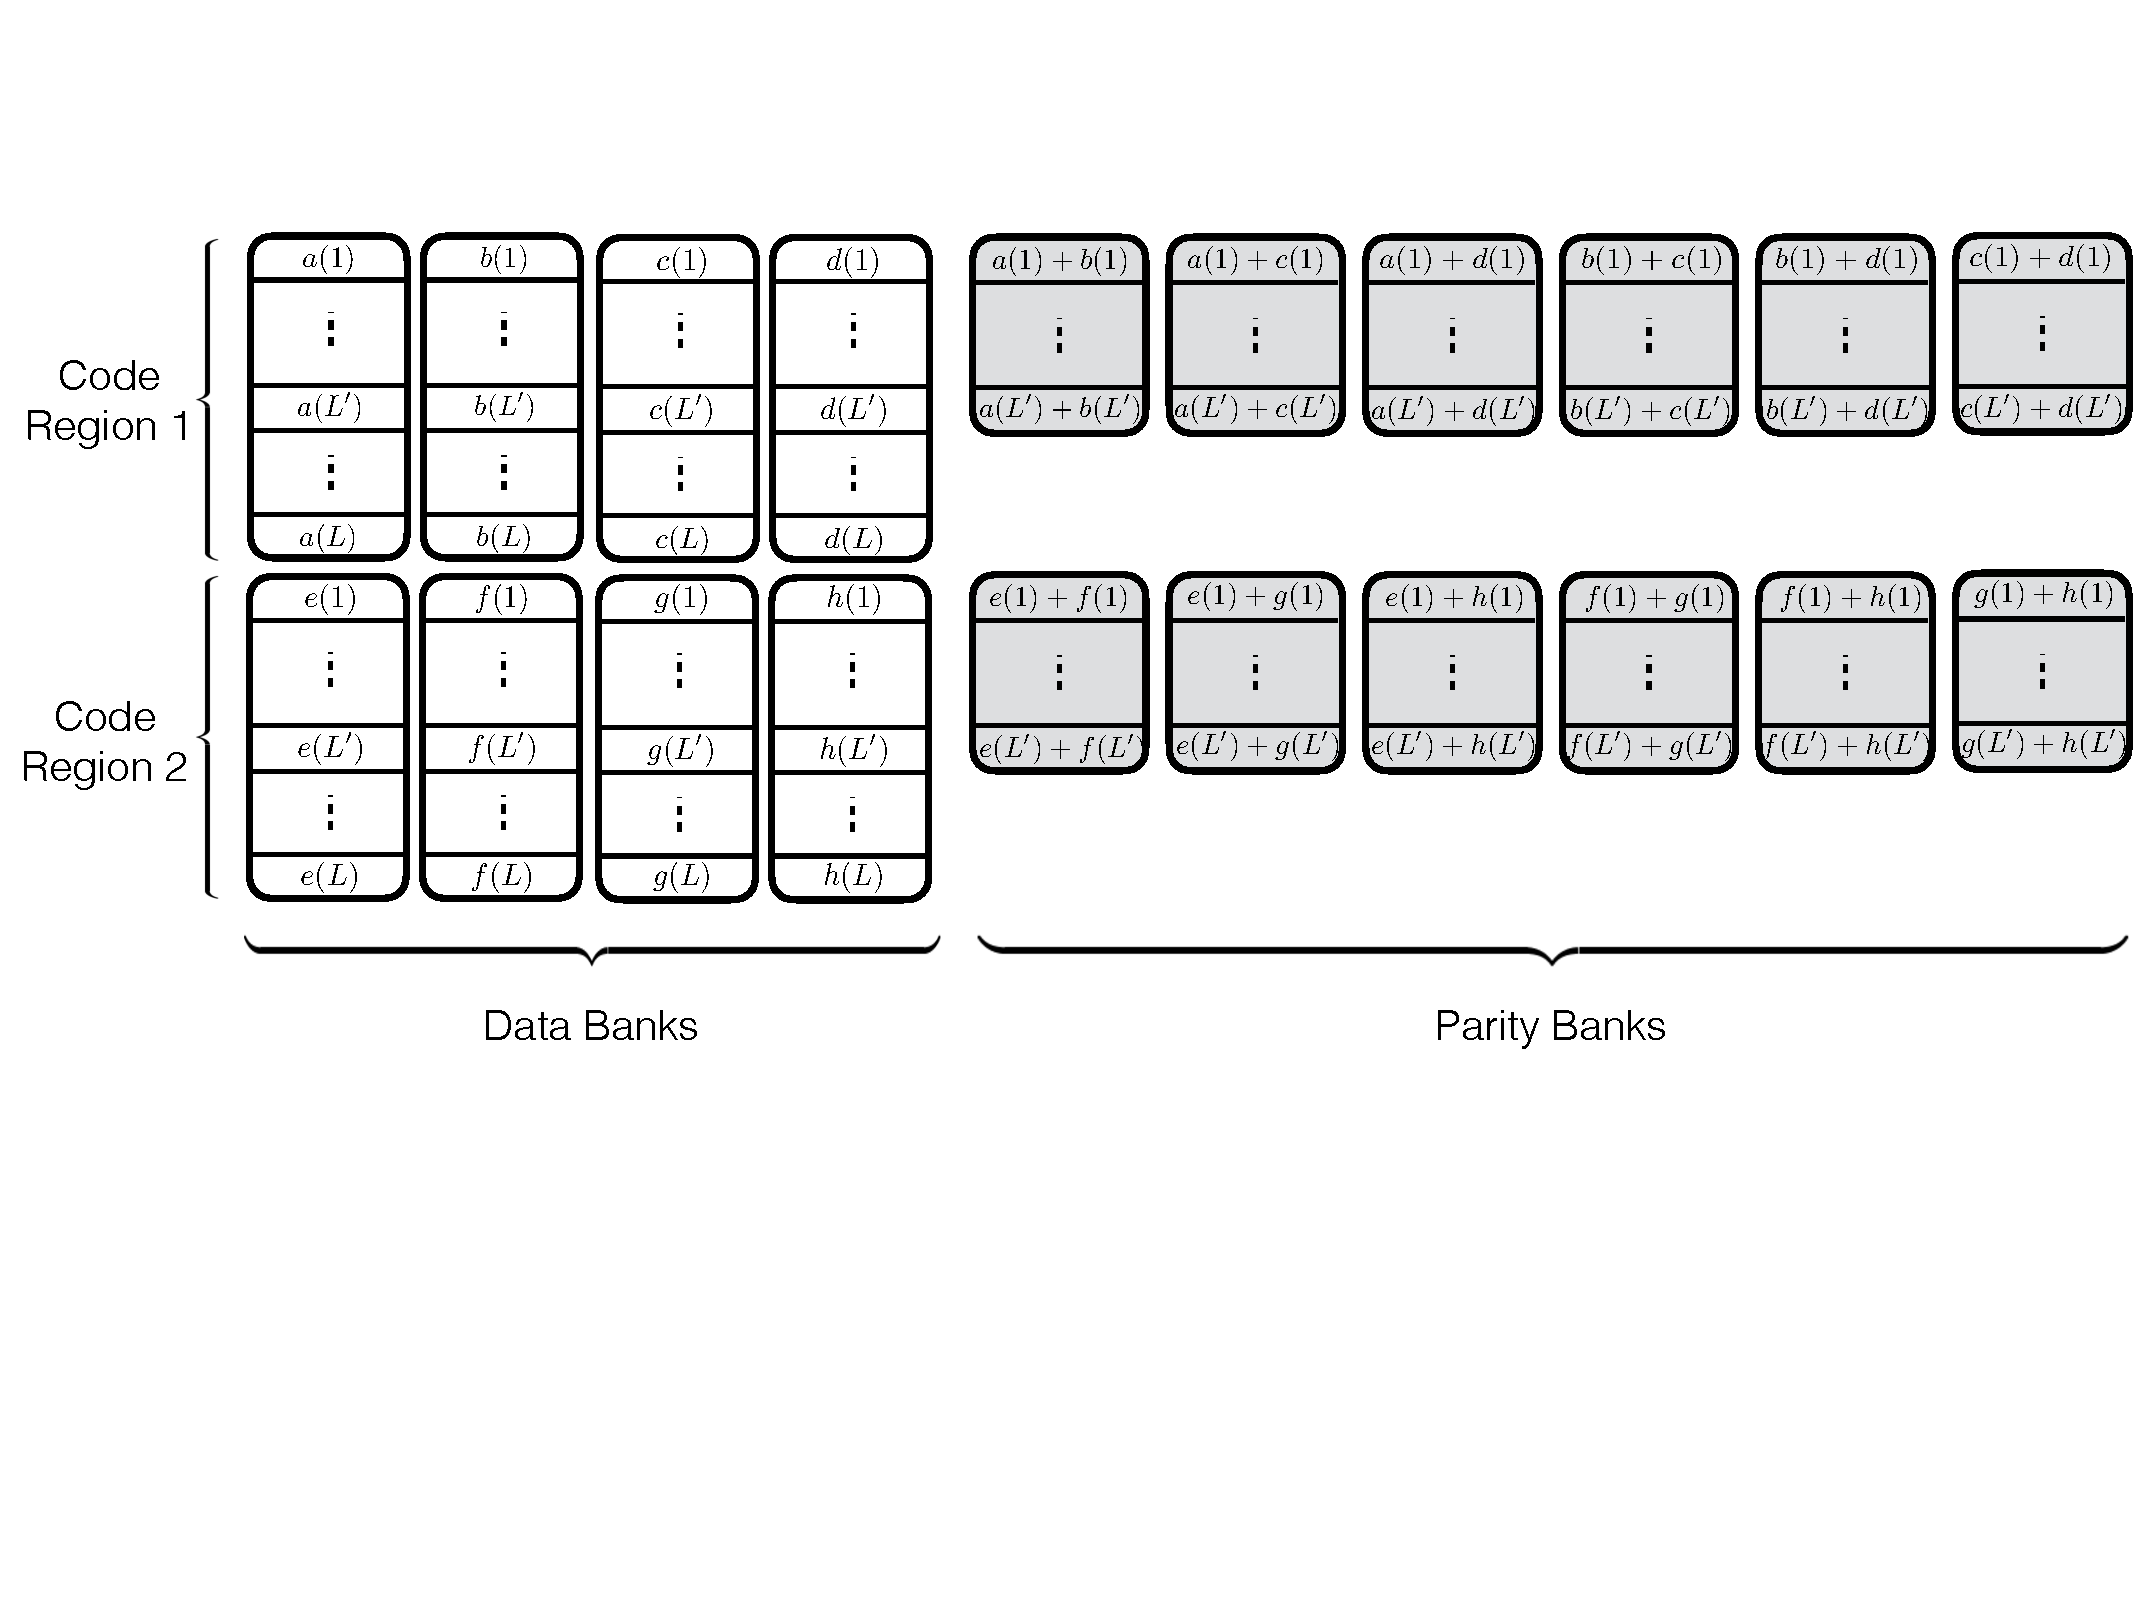
\includegraphics[width=1\linewidth]{fig/Code-Design-1.pdf}
	\caption{\it{Pictured here is an illustration of code scheme I.}}
	\label{fig:design1}
%\caption{Code Schemes}
\end{figure} 
%------------------------------
\ignore{
%------------------------------
\begin{figure}[ht!]
\centering
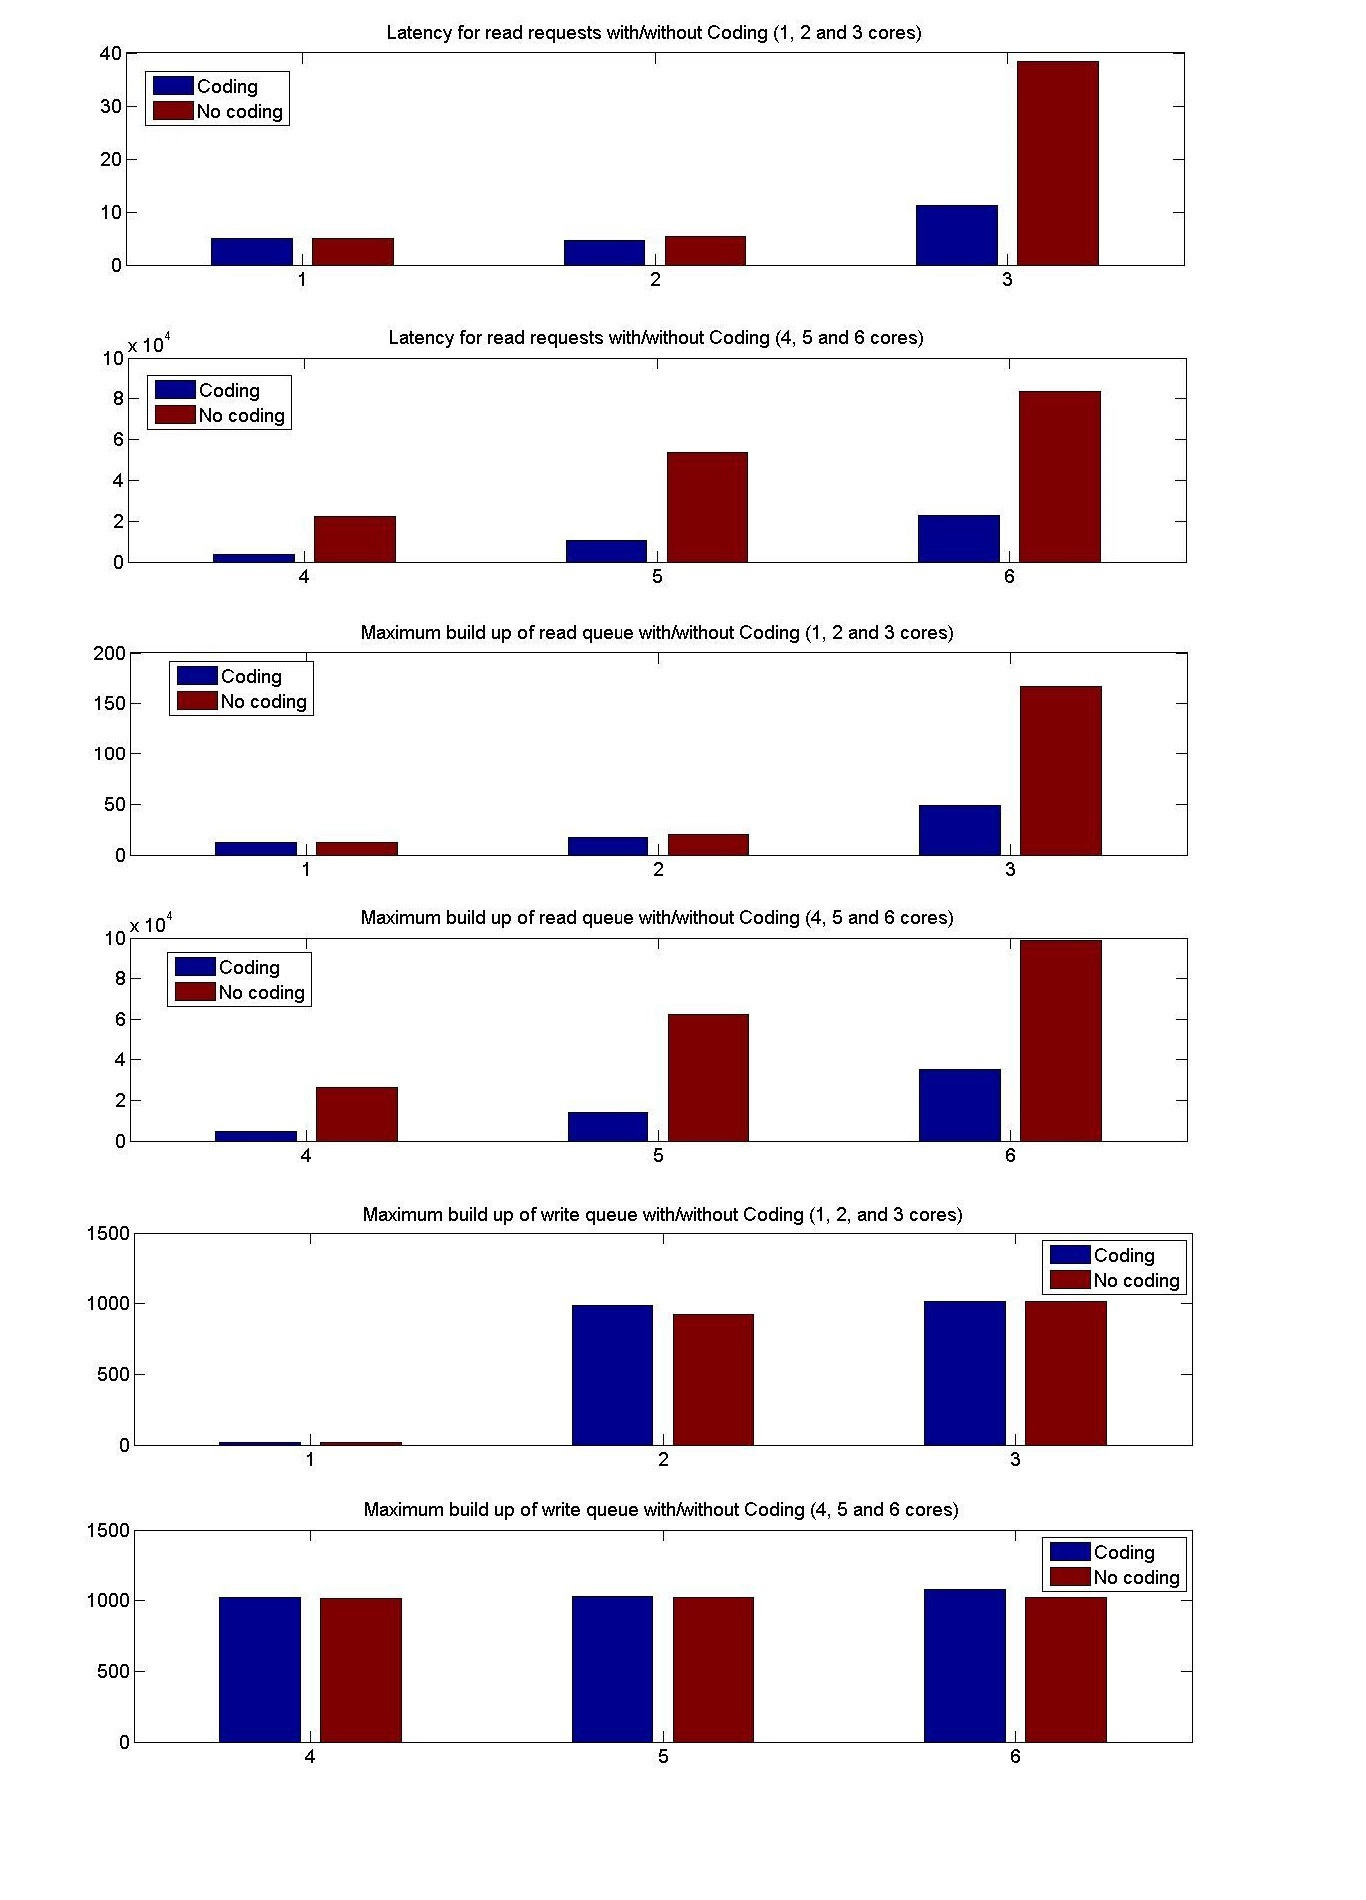
\includegraphics[width=150mm,natwidth=610,natheight=642]{fig/result_design1.jpg}
\caption{ }
\label{fig:result_design1}
\end{figure}
%------------------------------
}
\noindent \textbf{Worst case analysis}: This code scheme  (cf.~Figure~\ref{fig:design1}) may fail to utilize any parity banks depending on the requests waiting to be served. The worst case scenario for this code scheme is when there are non-sequential and non-consecutive access to the memory 
banks. Take for example a scenario where we only consider the first four banks of the code scheme. The following read requests are waiting to be served:  
\begin{align*}
\{a(1), a(2), b(8), b(9), c(10),c(11), d(14), d(15)\}. 
\end{align*}
Because none of the requests share the same row index, we are unable to utilize the parity banks. However, we still benefit from the prefetching mechanism discussed in Section~\ref{sec:prefetching}. The worst case number of reads per cycle is equal to the number of data banks. 
%In Figure~\ref{fig:result_design1} , we explore the worst case scenario when 
%the accesses are random. The results show that the queue build up for reads and 
%writes does fall back to no-coding scenario. This asserts that the worst case 
%scenario for a coding scheme performs similar to no-coding scheme.In the second 
%scheme, we augment the code storage by cross storing the codes from region 1 to 
%region 2 and vice-versa.We do this in addition to coding the consecutive memory 
%addresses in a bank. This provides two benefits, first it increases the overall 
%redundancy, and second it allows us to use the parity banks of the other region 
%in case the first region�s parity banks are in use. 
\ignore{
\begin{figure}[!ht]
\centering
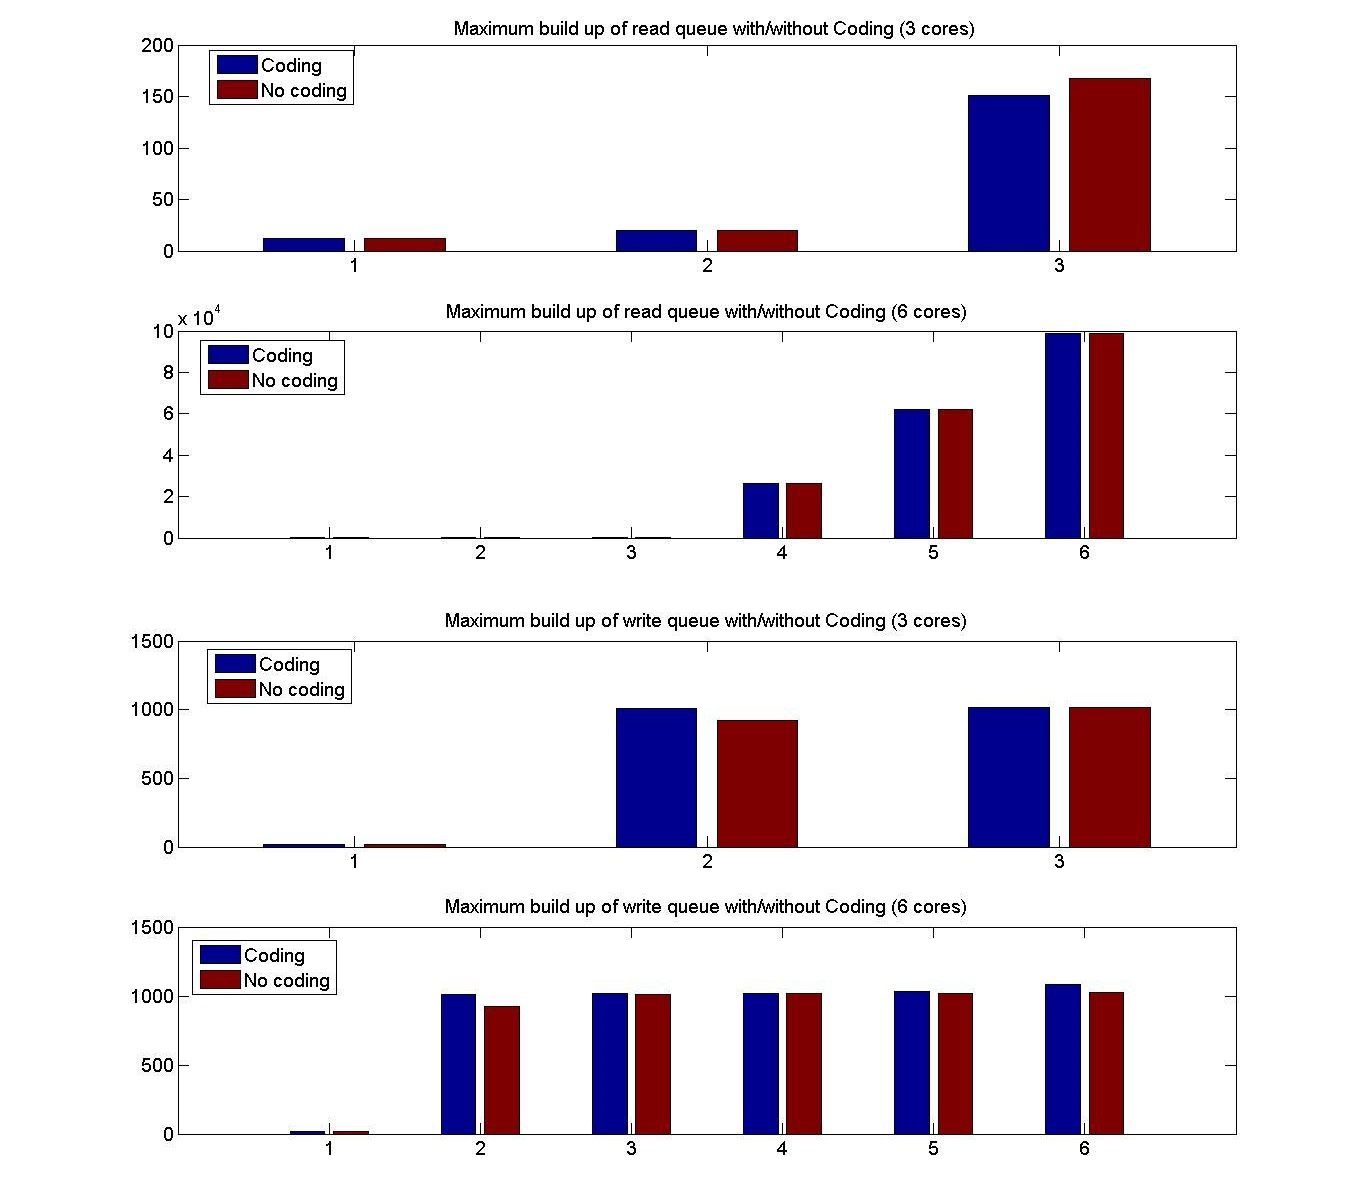
\includegraphics[width=150mm,natwidth=610,natheight=642]{fig/result_design2.jpg}
\caption{ Comparison of Design II with No coding case }
\label{fig:result_design2}
\end{figure}
}
\subsubsection{Code Scheme II}
\label{sec:design2}

Figure~\ref{fig:design2} illustrates the second code scheme explored in this paper. Again, the $8$ data banks $\{\mathbf{a}, \mathbf{b},\ldots, \mathbf{h}\}$ are partitioned into two groups containing $4$ data banks each. These two groups are then associated with two code regions. The first code region is similar to the previous code scheme, as it contains parity elements constructed from two data banks. The second code region contains data directly duplicated from single data banks. This code scheme further differs from the previous code scheme (cf. Figure~\ref{fig:design1}) in terms of the size and arrangement parity banks. Even though $L' = \alpha L$ rows from each data bank are stored in a coded manner by generating parity elements, the parity banks are assumed to be storing $2\alpha L > L'$ rows.

For a specific choice of $\alpha$, the storage overhead of this scheme is $20\alpha L$ which leads to a rate of $$\frac{8L}{8L + 20\alpha L} = \frac{2}{2 + 5\alpha}.$$ Note that this code scheme can support $5$ read accesses per data bank in a single memory clock cycle as opposed to $4$ read requests supported by the code scheme from Section~\ref{sec:design1}. However, this is made possible at the cost of extra storage overhead. Next, we discuss the performance of this code scheme in terms of the number of simultaneous read requests that can be served in the best and worst case.

%
%The second design, presented in figure 4, improves over first design by allowing 
%5 read accesses per bank per cycle. This design also divides banks into two 
%regions. The first region is
%Bank 1 to Bank 4 and 5 corresponding Parity banks. The two regions in figure 4 
%are upper 9 banks forming one region and lower 9 banks forming another. This 
%design allows intermix storage of parity among regions. The design uses 5 parity 
%banks per region. The data in this scheme is coded for both inter bank and 
%intra-bank. The intra-bank codes are stored in the alternate parity bank region. 
%This allows usage of parity banks from other region if they are available. \\
\begin{figure}[!ht]
%\centering
%\begin{minipage}[!t]{\linewidth}
	%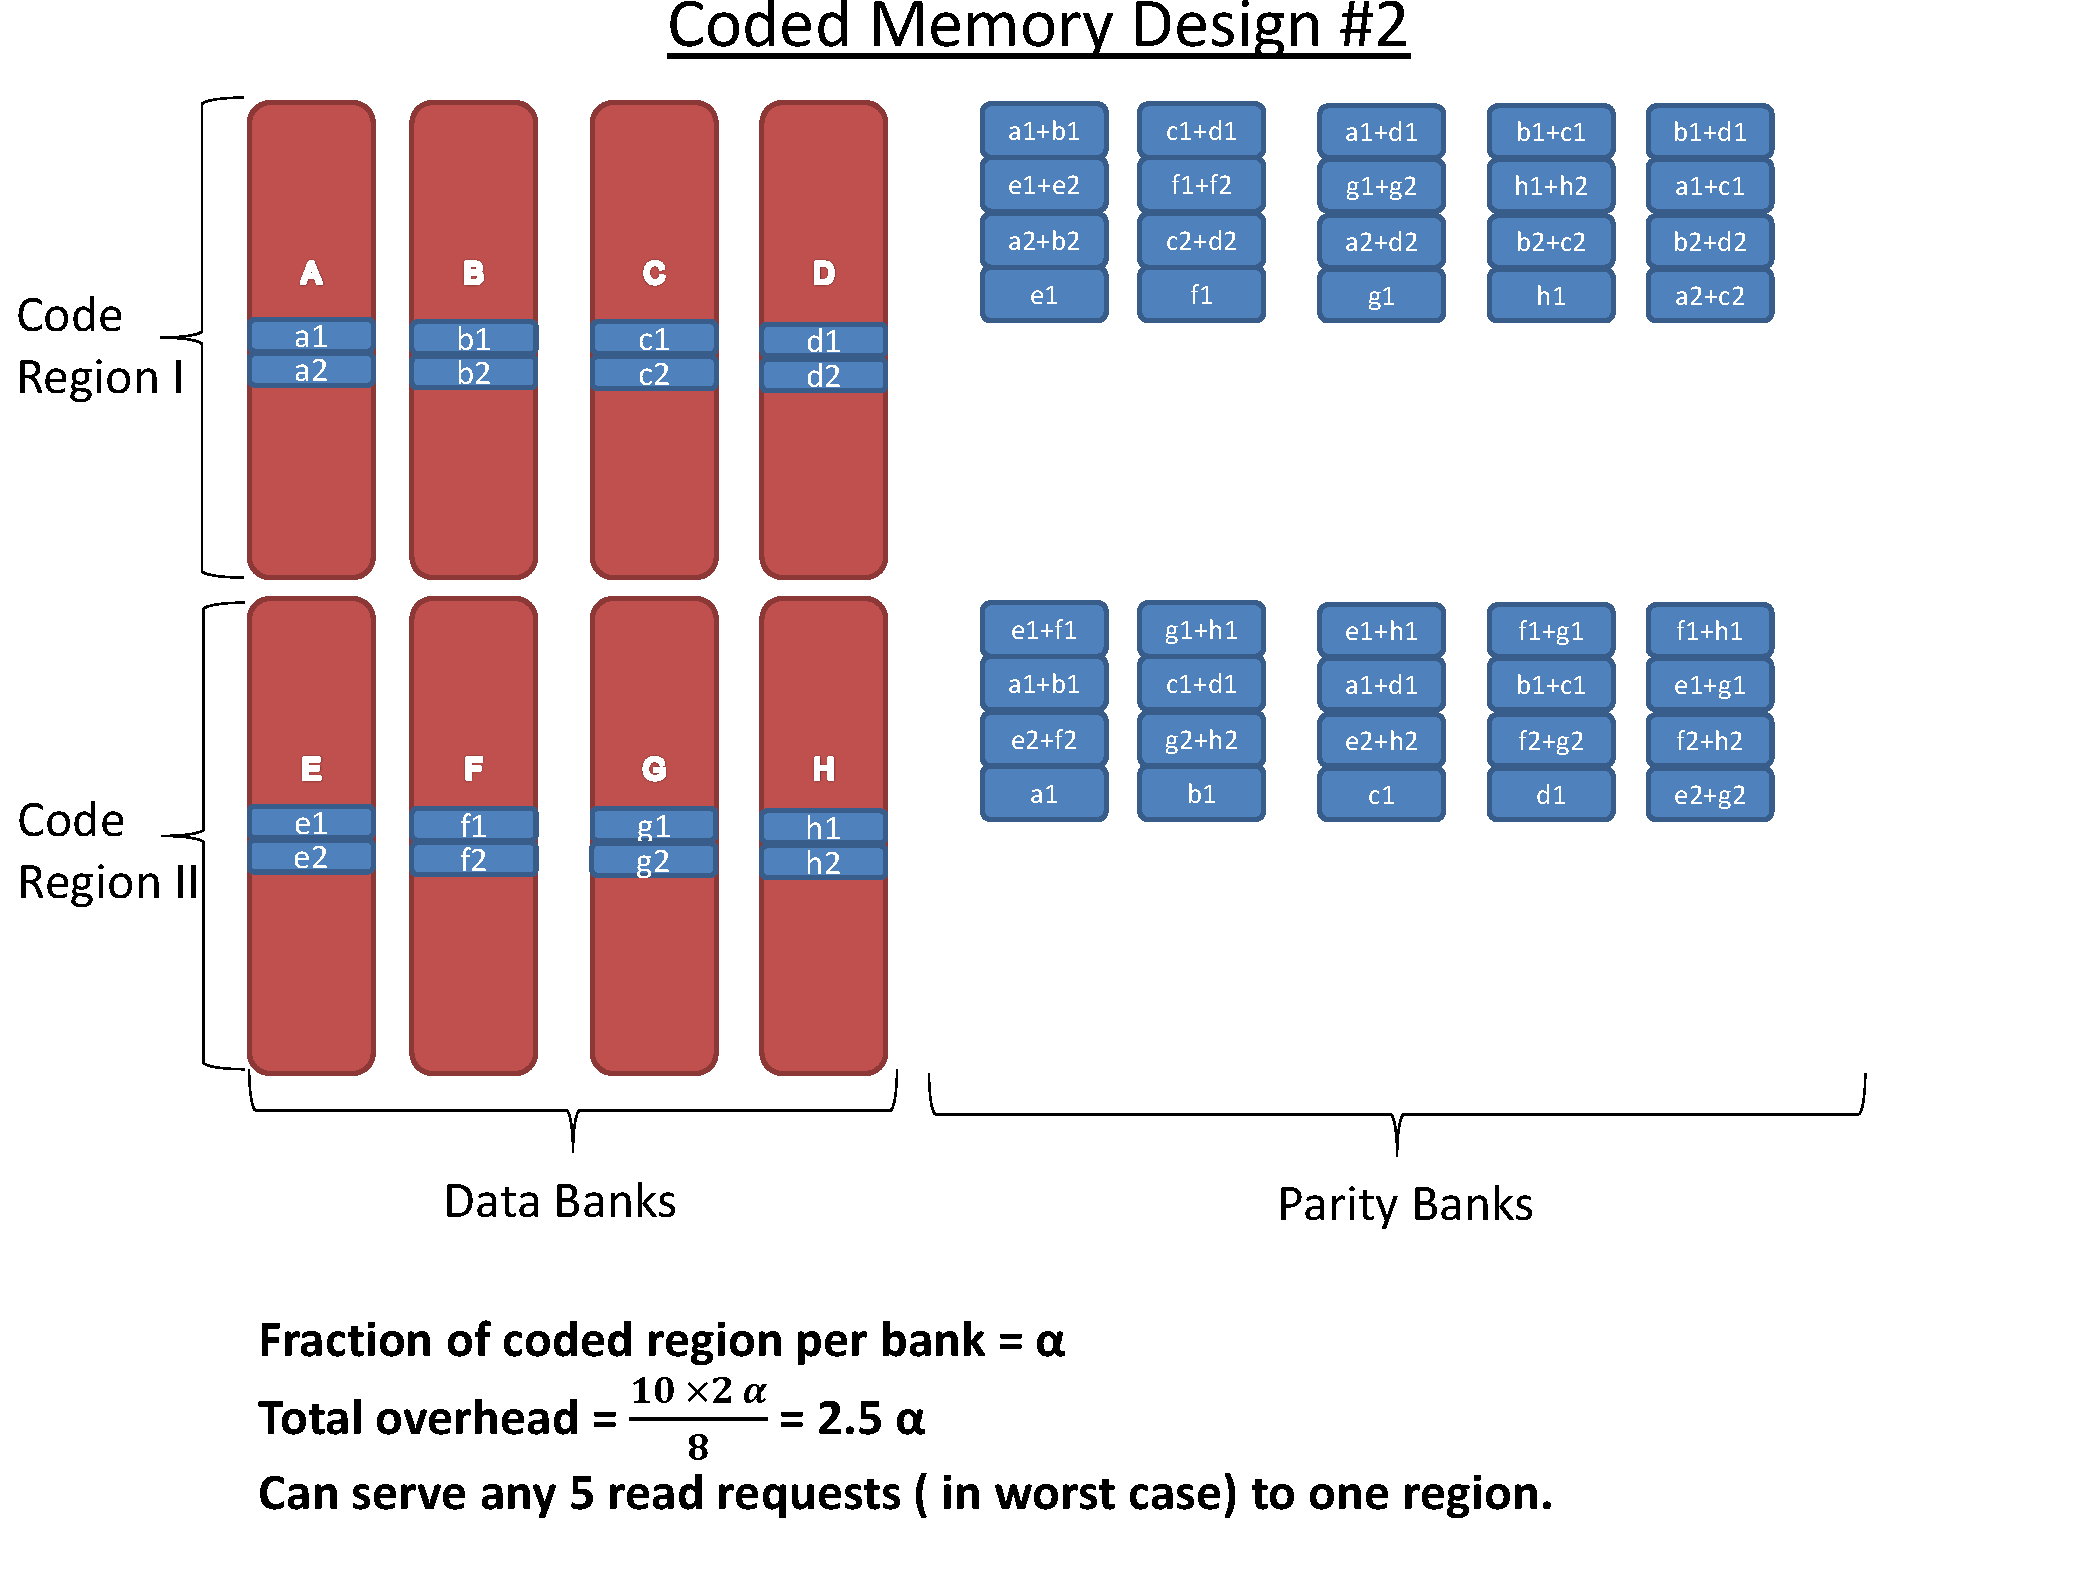
\includegraphics[width=1\linewidth]{fig/designII.pdf}
	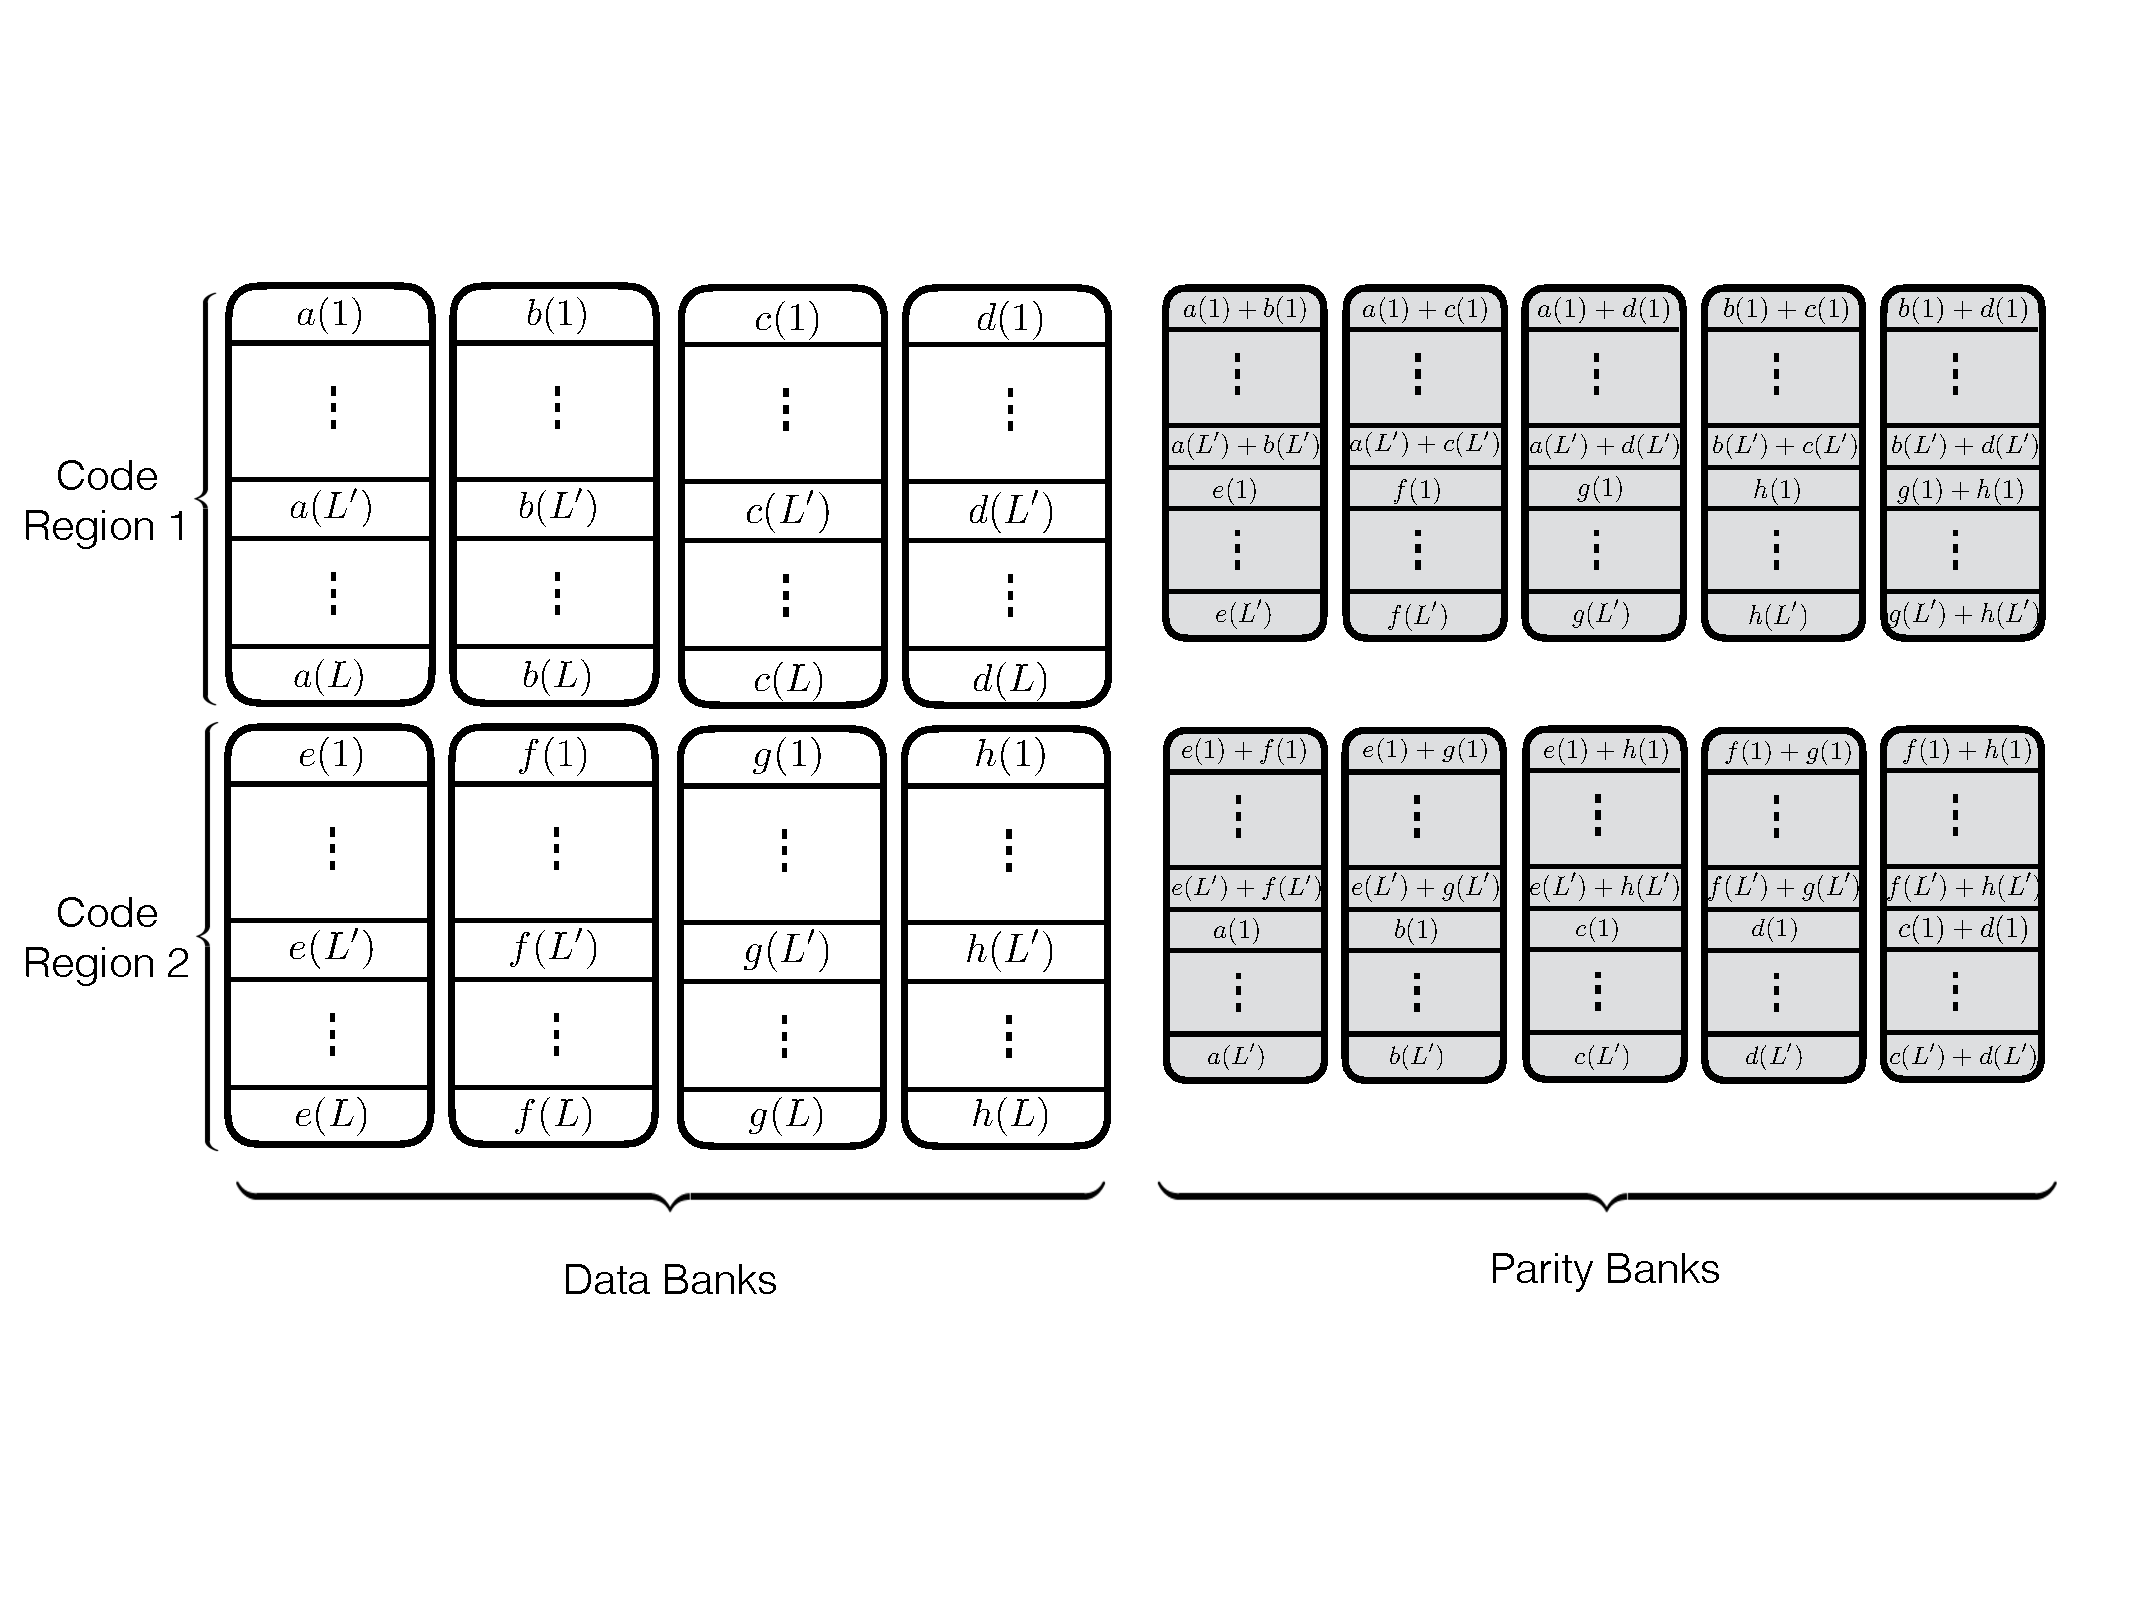
\includegraphics[width=1\linewidth]{fig/Code-Design-2.pdf}
	\caption{\it{Pictured here is an illustration of code scheme II.}}
	\label{fig:design2}
%\end{minipage}
\end{figure}

\noindent \textbf{Best case analysis:~} This code scheme achieves the best access performance when sequential accesses to the data banks are issued. In particular, this scheme can support up to $9$ read requests in a single memory clock cycle. Consider the scenario where we receive read requests for the following rows of the data banks. 
$$
\big\{a(1),b(1),c(1),d(1),a(2),b(2),c(2),d(2),a(3),b(3),c(3)\big\}
$$ Here, we can serve 
$\{a(1), b(1), c(1), d(1)\}$ using the data bank $\mathbf{a}$ with the parity banks storing the parity elements $\{a(1) + b(1),b(1)+c(1),c(1)+d(1)\}$. Similarly, we can serve the requests for the rows $\{a(2),b(2),d(2)\}$ using the data bank $\mathbf{b}$ with the parity banks storing the parity elements $\{a(2)+d(2), b(2)+d(2)\}$. Lastly, the request for the rows $c(2)$ and $d(3)$ is served using the data banks $\mathbf{c}$ and $\mathbf{d}$.\\


\noindent \textbf{Worst case analysis:~}The code scheme can enable $5$ simultaneous accesses in a single memory clock cycle in the
worst case. These are non-sequential and non-consecutive accesses to the memory banks. For 
example, when the access pattern corresponds to the rows $\{a(1),b(6),c(9),d(15),e(20)\}$, we can simultaneously serve 
these $5$ read requests with the help of our coded memory. In order to better utilize the unused banks in this case, we can use the prefetching 
mechanisms (cf. Section~\ref{sec:prefetching}) to look ahead in the queue and proactively download elements from the unused banks for future accesses.


% This design employs both inter-bank and intra-bank encoding in order to generate the content to be stored on the parity banks. In order to illustrate another flexibility that can be utilized while designing the storage space for a memory system, even though this code scheme encodes $\alpha L$ rows from each data bank, the parity banks are assumed to be storing $2\alpha L$ rows.


\subsubsection{Code Scheme III}
The next code scheme we discuss has locality 3, so each degraded read requires two parity banks to be served. This code scheme works with $9$ data bank $\{\mathbf{a}, \mathbf{b},\ldots, \mathbf{h}, \mathbf{z}\}$ and generates $9$ shallow parity banks. Figure~\ref{fig:design3} shows this scheme.
%The two designs discussed above achieve a rate of $2/5$. Here, we explore a code scheme which achieves a rate of $1/2$. 
%This design requires 9 data banks and 9 parity banks as shown in figure 5. It 
%also has a comparatively higher locality of 3. That is, it requires the memory 
%controller to "know" two out of three data elements to decode the third. 
The storage overhead of this scheme is $9\alpha L$ which corresponds to the rate of $\frac{1}{1 + \alpha}$. We note that this scheme possesses higher logical complexity as a result of its increased locality. 

This scheme supports $4$ simultaneous read access per bank per memory clock cycle as demonstrated by the following example. Suppose rows $\{a(1), a(2), a(3), a(4)\}$ are requested. $a(1)$ can be served directly from $\mathbf{a}$. $a(2)$ is served by means of a parity read and reads to banks $\mathbf{b}$ and $\mathbf{c}$, $a(3)$ is served by means of a parity read and reads to banks $\mathbf{d}$ and $\mathbf{g}$, and $a(4)$ is served by means of a parity read and reads to banks $\mathbf{e}$ and $\mathbf{z}$.

\noindent \textbf{Best case analysis:~} Following the analysis similar to Code Schemes I and II, the best case number of reads per cycle will be equal to the number of data and parity banks.

\noindent \textbf{Worst case analysis:~} Similar to coding schemes I and II, the number of reads per cycle is equal to the number of data banks. 
%The memory overhead here is less (just $\alpha$) compared to the previous designs. However, it possesses higher logical complexity because of increased locality. Example cases for this design are described below :
%\begin{itemize}
%
%	\item 4 reads for $a_0$: 1 read from $a_0$, 1 read from ($a_1$, $a_2$, 
%		$a_0$ + $a_1$ + $a_2$), 1 read from ($a_3$, $a_6$, $a_0$ + $a_3$ 
%		+ $a_6$), and the 4th read from ($a_4$, $a_8$, $a_0$ + $a_4$ + 
%		$a_8$).
%	\item 3 reads for $a_0$: 1 read from $a_0$, 1 read from ($a_3$, $a_6$, 
%		$a_0$ + $a_3$ + $a_6$), and the 3rd read from ($a_4$, $a_8$, 
%		$a_0$ + $a_4$ + $a_8$). \\
%	      1 read for $a_1$:  1 read from $a_1$.
%	\item 2 reads for $a_0$: 1 read from $a_0$ and the 2nd read from ($a_3$, 
%		$a_6$, $a_0$ + $a_3$ + $a_6$). \\
%	      2 reads for $a_1$: 1 read from $a_1$ and the 2nd read from ($a_4$, 
%	      $a_7$, $a_1$ + $a_4$ + $a_7$).
%	\item 2 reads for $a_0$: 1 read from $a_0$ and the 2nd read from ($a_3$, 
%		$a_6$, $a_0$ + $a_3$ + $a_6$). \\
%	      1 read for $a_1$: 1 read from $a_1$. \\
%	      1 read for $a_2$: 1 read from $a_2$.
%    \end{itemize}
%---------------------------------------
\begin{figure}[!ht]
	\centering
	\begin{minipage}[!t]{\linewidth}
		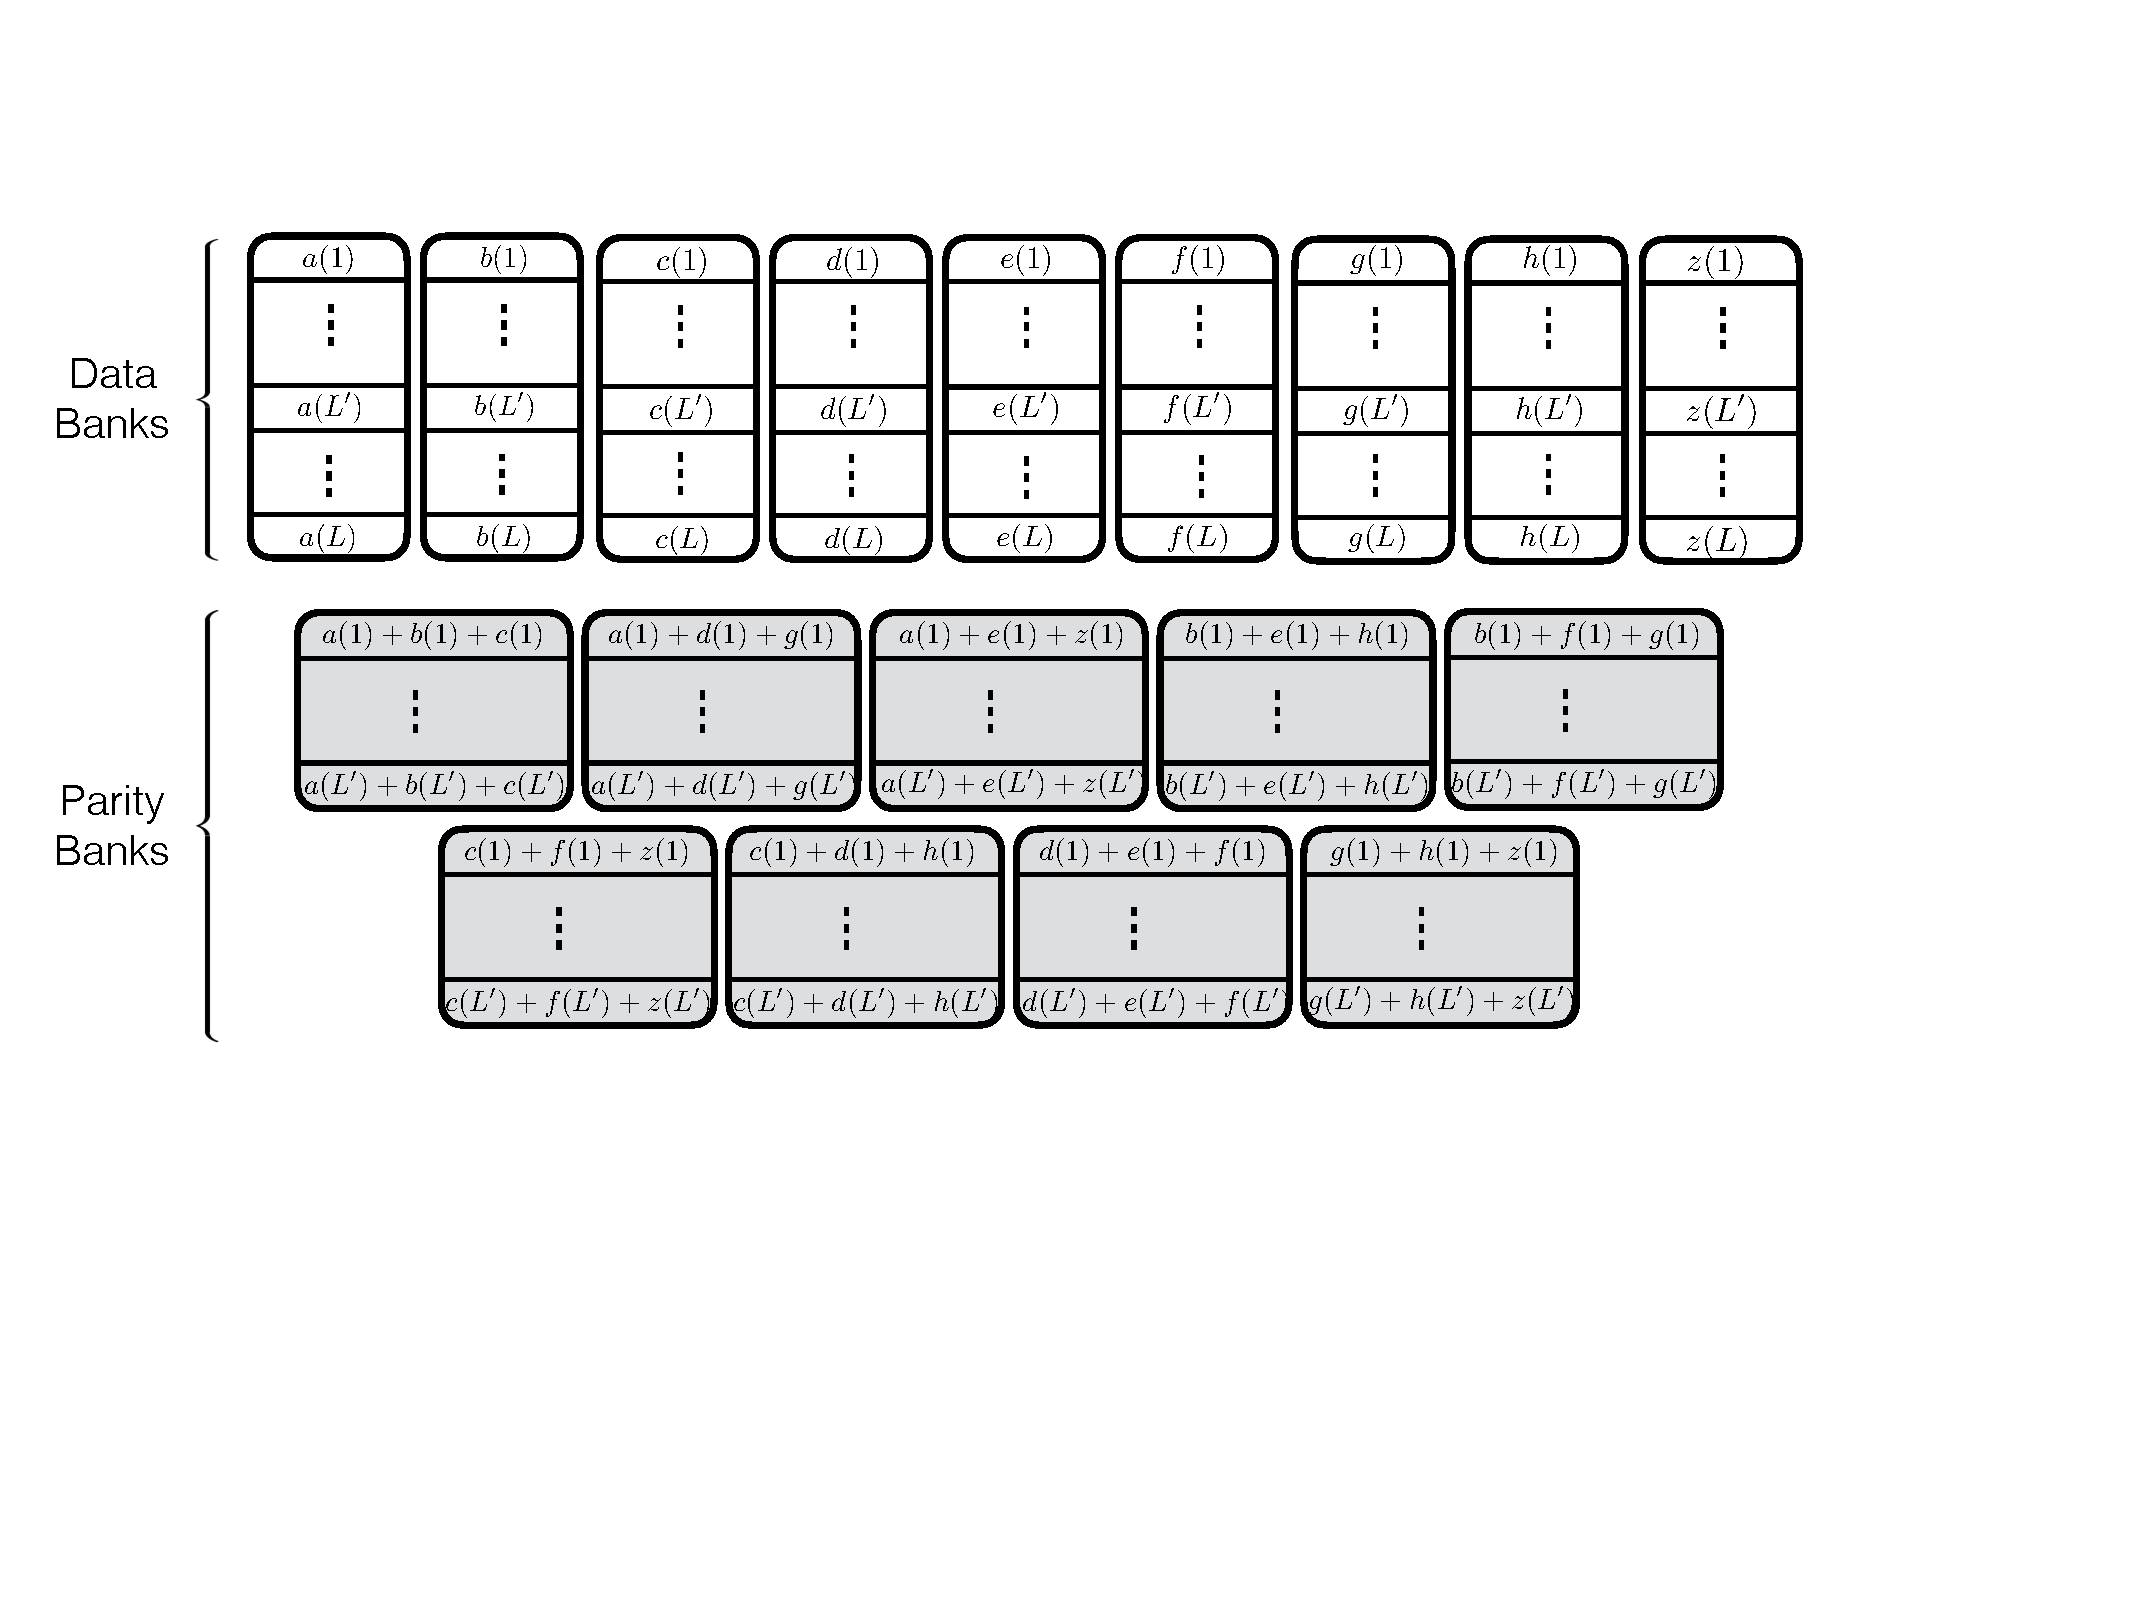
\includegraphics[width=\linewidth]{fig/Code-Design-3_9banks.pdf}
		\caption{\it{Pictured here is an illustration of code scheme III.}}
		\label{fig:design3}
	\end{minipage}
\end{figure}
%---------------------------------------

\begin{remark}
Note that the coding scheme in Figure~\ref{fig:design3} describes a system with $9$ data banks. However, we have set out to construct a memory system with $8$ data banks. It is straightforward to modify this code scheme to work with $8$ data banks $\{\mathbf{a}, \mathbf{b},\ldots, \mathbf{h}\}$ as shown in Figure~\ref{fig:design3_8}.
%Since most systems are implemented with number of banks as $2^n$ for some n. We present an 
%example of the code with 8 data banks in figure~\ref{fig:design3_8}. For using 8 data banks, 
%we drop the bank I. We also ignore the data from Bank I for constructing parity. So, three of 
%the parity banks have the locality of 2, while the rest of the parity banks have locality of 3.
% The new scheme for 8 data banks has 9 parity banks.
 \end{remark}
%---------------------------------------
\begin{figure}[!ht]
\centering
	\begin{minipage}[!t]{\linewidth}
		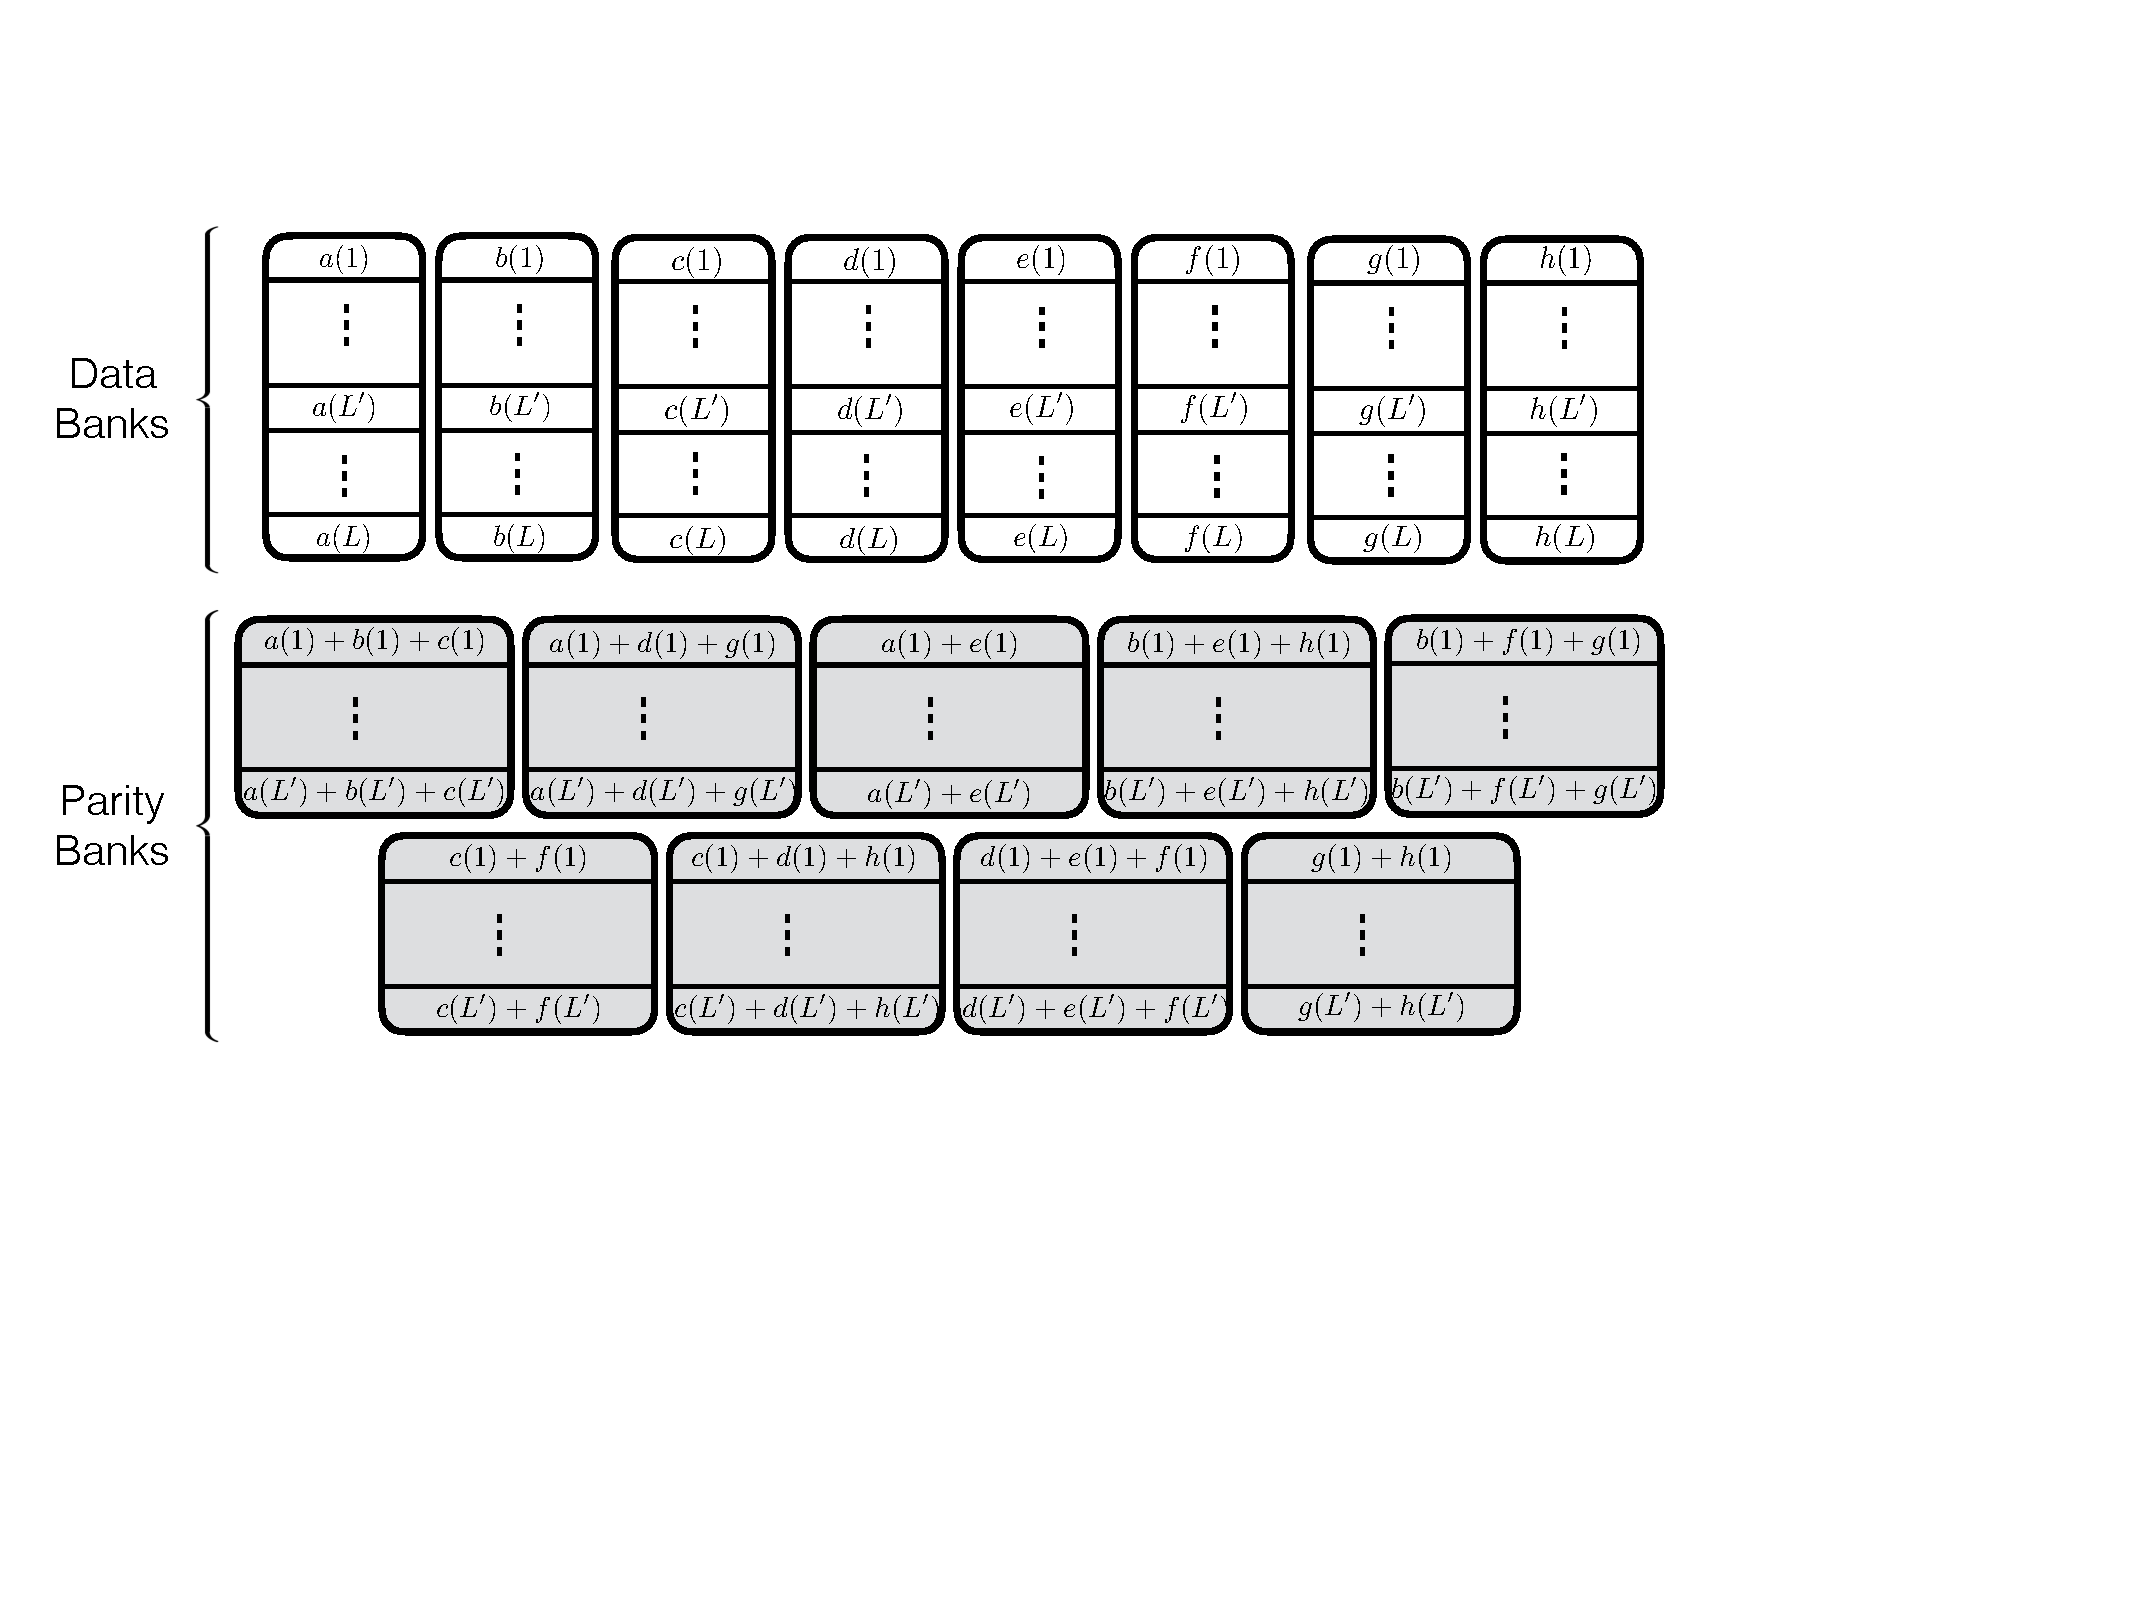
\includegraphics[width=\linewidth]{fig/Code-Design-3_8banks.pdf}
		\caption{\it{Pictured here is an illustration of code scheme III with 8 data banks.}}
		\label{fig:design3_8}
	\end{minipage}
\end{figure}
%---------------------------------------

\begin{comment}
Since the locality is 3 here in this design, i.e. , each parity is made up of combination of 3 data banks, we need to make sure that all three requests are in one line to be able to use the parity bank. 
For example parity bank 0 contains A+B+C. So, the following scenarios arise:
\begin{itemize}
	\item {\em Scenario I}: 1st request of A and 1st request of B are in same row. Then, we can search for a request in the same row for bank C by doing a look ahead. 
	\item {\em Scenario II}: 1st request of A and 1st request of C are in same row. Then, we can search for a request in the same row for bank B by doing a look ahead. 
	\item {\em Scenario III}: 1st request of B and 1st request of C are in same row. Then, we can search for a request in the same row for bank A by doing a look ahead. 
\end{itemize}
So, the simple pseudo code for doing this would be :\\
\begin{verbatim}
for each data bank 
    for each auxiliary bank1 of data bank
            Look ahead in auxiliary bank2 and check if 3 request in a row.
        end
    end
\end{verbatim}
Example: - \\
For {\bf data bank} to be {\bf A} \\
{\bf auxiliary bank1} goes from [B C D G A E] \\
{\bf auxiliary bank2} goes from [C B G D E A] \\
  The element A is just there in {\bf auxiliary bank1} and {\bf auxiliary bank2} to maintain the symmetry because A + E has locality of 2.
\end{comment}


%In this section, we explore the technique of dynamic coding in order to reduce the memory and access overhead associated with the parity banks. We first discuss the scheme of dynamic coding and follow it by discussing the potential benefits of prefetching the codes.\\
\underline{\textit{Dynamic Coding}}:
The contention in memory accesses from various cores occurs mostly when the access are to shared-memory, especially when they are localized to certain memory regions. We explore the locality of the memory access over a period of time to reduce the memory overhead for storing the codes. In a multi-core system, when various cores try to work from a shared memory location, they tend to generate accesses to a localized region of memory. This motivates the idea of coding the localized region during the period of heavy access, and dynamically changing the region whenever there is change in the locality of memory accesses.
Figure~\ref{fig:dsp_access1} shows the access pattern of the LTE cores 0 to 6. The y-axis of the figure shows the address accessed by the LTE cores over a period of time. The x-axis denotes the time in nanoseconds. This plot shows that most of the access from various cores are limited to the memory range from 0x007a1200 to 0x00c65d40 (lower and higher range on the y axis). It also suggests that most (about 60$\%$) of the accesses belong to the memory region of 0x00a037a0 to 0x00b71b00. \\
We make similar observation from Figure ~\ref{fig:dsp_access2} for UMTS. We observe a highly concentrated access pattern in case of UMTS. Here again, all of the access for a duration of approximately 0.2 ms is in the address range of 0x007a1200 to 0x01036640. \\
Figure~\ref{fig:bank_access1} shows a view of memory accesses from the bank's side. It shows the access request pattern for each of the memory bank. The concentration of accesses to a region is observed across memory banks. This makes us conclude that the memory banks can be parallely coded for a particular region as shown as green and yellow color in ~\ref{fig:design1}

\begin{figure}[ht!]
\centering
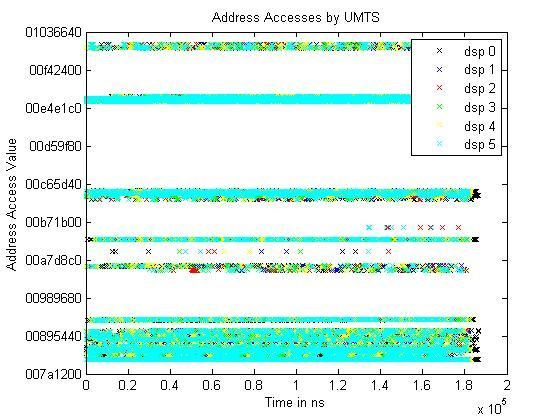
\includegraphics[width=150mm,natwidth=610,natheight=642]{core_access2.jpg}
\caption{ Comparison of Design II with No coding case }
\label{fig:dsp_access2}
\end{figure}
\begin{figure}[ht!]
\centering
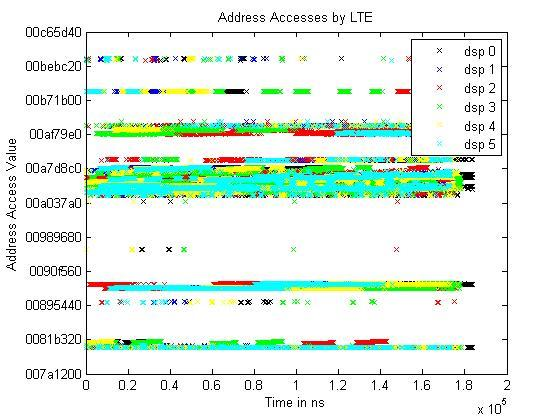
\includegraphics[width=150mm,natwidth=610,natheight=642]{core_access1.jpg}
\caption{ }
\label{fig:dsp_access1}
\end{figure} 
\\
From the above observations, we demonstrate the idea of coding the highly accessed portion of the memory. This scheme benefits from a huge reduction of the memory overhead with coding. The reduction the memory overhead can be used to reduce the complexity of the decoder by using simple coding functions (e.g. xor) and for densely coding (e.g. repeatedly coding a single element using 2 elements). \\
The scheme of dynamic coding requires that the currently coded region changes when the access pattern changes. That is, the localized memory area that is most heavily accessed can change, and it will require the system to recode the new localized access region. We assume that the working area of a program changes with change in the input parameters to the program. It can be easily observed from the above figures that the working area or the localized area is constant for at least 0.2 ms. This suggests that the switching of the coded region is not very frequent. During these periods of coding switches, it is also guaranteed that the number of accesses served from the memory is at worst equal to the number of banks available. In other words, coding the memory has no performance degradation compared to non-coding during these times. The system also needs to maintain an algorithm to observe the access pattern of the cores, and make a decision when it is time to code a new memory region. To do this, the memory controller tracks the most accessible region during a time period and makes a decision to slide/shift the coded region. This shift in the coded region requires the update of the parity bank for the new region. This process is carried out in conjunction with the ongoing access to the newly coded region. Therefore, this operation only requires writes to the parity banks, since we can use the current reads from the coded region to access the data that is to be coded. In addition, reads are also scheduled in the idle periods, when there is no read or write request to the bank/banks.\\
Dynamic coding requires the system to divide the memory into sub-regions and to keep track of accesses in these sub-regions. Once the number of accesses to a sub-region reaches a given threshold, it must then make this region the currently coded area. We propose this mechanism based on window concept. The system maintains a tuple of sub-regions such as [Starting Address, Length]. Each sub-region is thus given a starting address and length. Any access to a particular sub-region is considered as a hit. The system has a hit counter associated with each of the sub-region which is incremented for each hit. The system makes a decision of coding a particular sub-region based on its counter value. The number of coded sub-regions at a particular time is based on the sub-region size and the code storage size. The eviction of a coded region follows the Least Recently Used (LRU) policy similar to cache.\\
\begin{figure}[ht!]
\centering
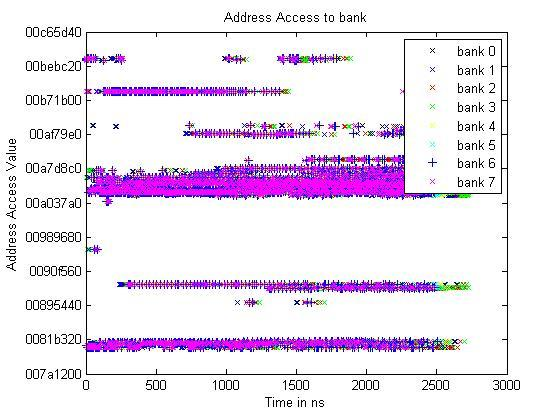
\includegraphics[width=150mm,natwidth=610,natheight=642]{bank_access.jpg}
\caption{ shows the access to banks }
\label{fig:bank_access}
\end{figure} 
\underline{\textit{Prefetching Codes}}:
The technique of dynamic coding reduces the memory overhead by exploiting the localized nature of memory accesses from the cores. In this section, we explore prefetching the coded data to reduce the access overhead caused for fetching the codes. This is done by exploiting the gaps in the memory access to any bank and using these gaps to prefetch the code/data for a future memory access. During a program, there are access cycles when certain banks do not have any access scheduled for a read/write. We propose the prefetching technique where we look forward in the queue and anticipate a pre-fetch for the data/code for that bank. We explore the implementation of a memory prefetching unit, similar to an instruction or cache prefetching unit. This unit can detect linear access patterns to regions in memory.  For example, if a string of memory accesses are issued in sequential byte sized order, then the prefetching unit will predict the next access to be in byte increments. The memory prefetching works by fetching a predicted address from the parity bank during accesses that the parity bank is idle. When future memory accesses are issued, they are first checked with the pre-fetched data to see if they can be used to decode any subsequent accesses memory accesses. If so, the memory access is obtained from the current accesses and pre-fetched data. For example, say the pre-fetcher sees 2 consecutive memory requests in a row. It then predicts that the next two accesses, locations $a_0$ and $b_0$, are likely to be accessed in the near future. It reads $a_0+b_0$ from the parity bank for future use. Next, access to location $a_0$ and $b_0$ are issued to the memory. Now, instead of reading both $a_0$ and $b_0$, only a single location has to be read from in memory, while the other location can be obtained from the pre-fetched data. This allows for an additional access to be issued from the now free memory bank.  In these cases, it is possible to obtain up to two additional memory accesses in a given cycle, one from the pre-fetched data and one from the parity bank.
\begin{figure}[ht!]
\centering
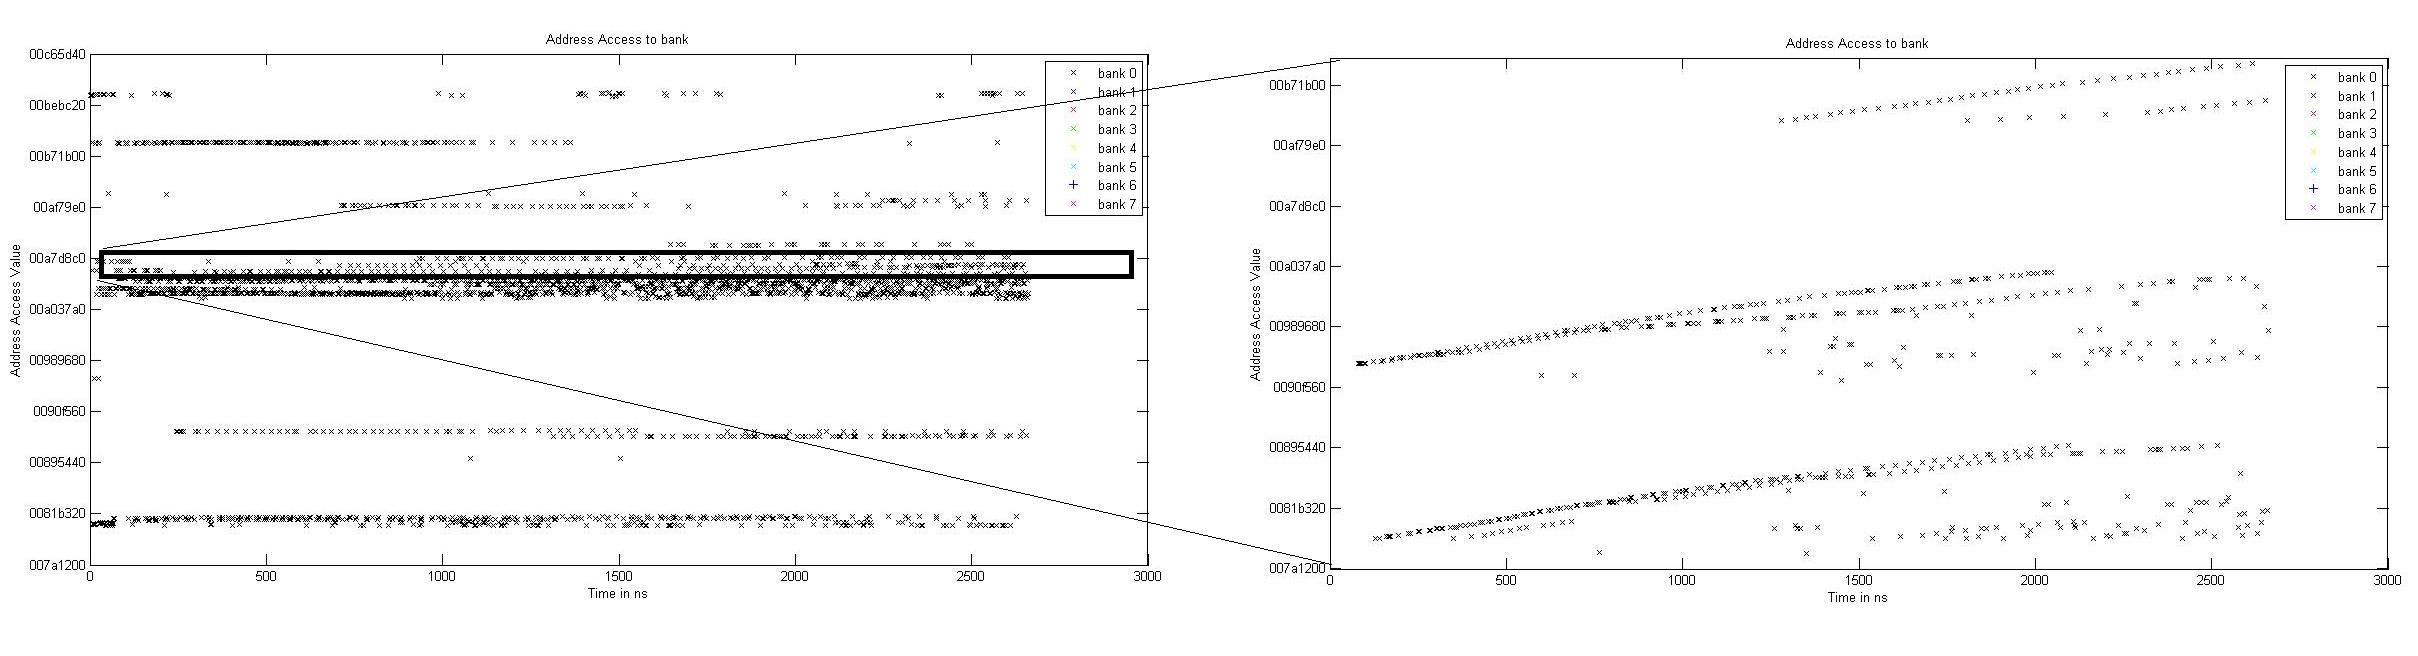
\includegraphics[width=150mm,natwidth=610,natheight=642]{bank_access1.jpg}
\caption{ }
\label{fig:bank_access1}
\end{figure} 
Implementation of a memory prefetch should only require overhead for space and the associated logic to implement it. Since memory accesses are often stalled due to bank conflicts, checking pending accesses to the pre-fetched data should require no additional time overhead. As memory accesses wait to be issued in the bank queues, they can simultaneously be checked with the pre-fetched data. Thus, no extra latency is anticipated by the addition of a memory prefetching unit.
Figure~\ref{fig:bank_access1} shows two plots of memory accesses to a bank with respect to time. The left figure shows the accesses to the memory bank by various cores. The right side figure shows a zoomed view of the accesses in the dense access region. This figure suggests the linearity of accesses. The system can look ahead in the queue to detect the consecutive address request for a memory bank and schedule a prefetch of the associated code. 
\begin{figure}[ht!]
\centering
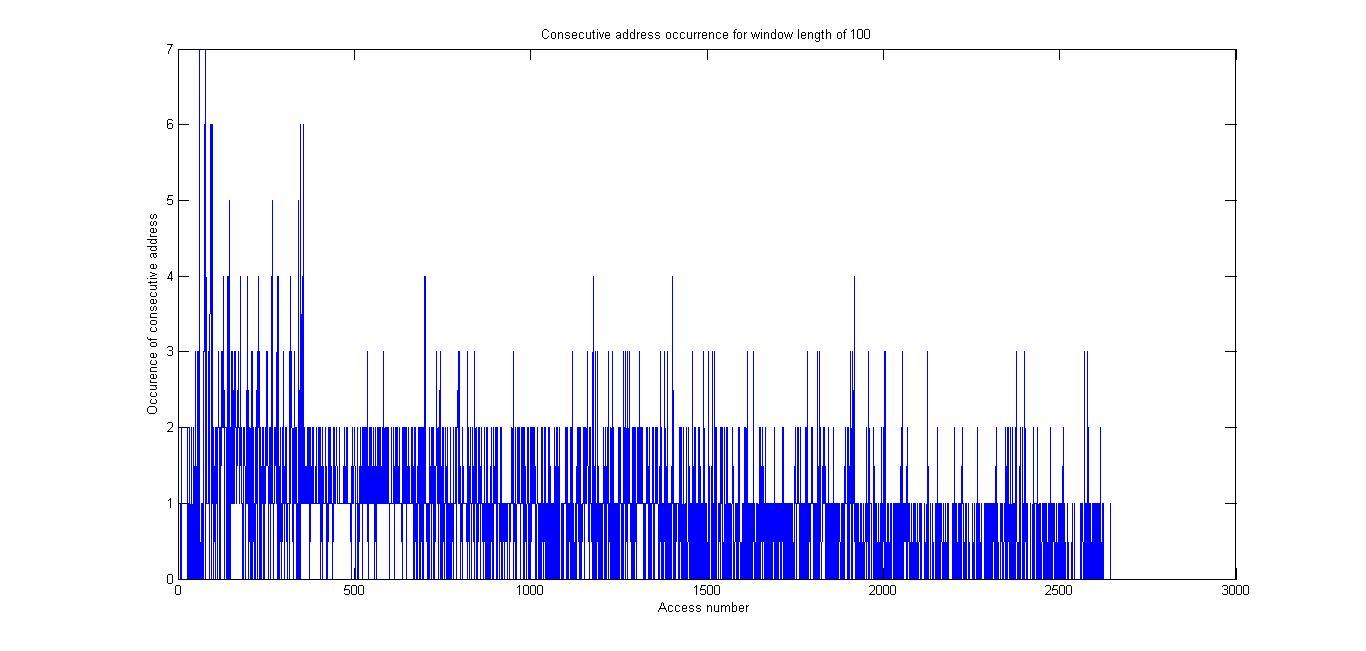
\includegraphics[width=150mm,natwidth=610,natheight=642]{queue_lookahead.jpg}
\caption{ }
\label{fig:queue_lookahead}
\end{figure} 
In figure~\ref{fig:queue_lookahead}, we simulate the prefetching of the code by using a window of length 100. That is, we look ahead to 100 requests in the queue and find out the occurrence of consecutive address in the window. The plot suggest high occurrence of the consecutive addresses in the bank which can be served by prefetching the codes.  


%\section{Memory Controller Design}
\label{sec:memcontrol}
%\Matt{BLUE: I would not mind removing this text. RED: I will likely remove this text}
The architecture of the memory controller is focused on exploiting redundant storage in the coding schemes to serve memory requests faster than an uncoded scheme.
%The memory design involves two key components: 1) storage space comprising of memory banks and 2) memory controller 
%The coding schemes discussed in previous section is implemented using systemC. 
%This section describes the architectural detail of how the schemes are 
%implemented using optimized algorithms. \\
%In this section, we explore the technique of dynamic coding in order to reduce 
%the memory and access overhead
%associated with the parity banks. We first discuss the scheme of dynamic coding 
%and follow it by discussing the potential benefits of prefetching the codes.\\
%\subsection{Memory Controller Stages}
%A general memory controller consists of three stages of processing illustrated in Figure~\ref{fig:multicore_arch}. The first stage, the {\em core arbiter}, receives memory access request from the master cores. The core arbiter then routes the requests to the proper {\em bank queue}. The bank queues are the second stage of processing, and they are responsible for storing and tracking memory requests. A memory request seeking memory located in bank $N$ will be sent to the $N$th bank queue. The {\em access scheduler} is the final stage of processing. It is responsible for scheduling the requests in the bank queues. Each memory cycle, the access scheduler generates an access pattern based on the requests present in the bank queues. The access pattern is a description of the reads or writes the memory controller will perform on the memory banks. Next, we discuss all of these three units and their functions in a greater detail.
%first level is {\em Core Arbiter }, the unit responsible for handling requests 
%from cores.  The second level is {\em Bank Arbiter} responsible for arbitrating 
%requests to banks.  The third level is {\em Access Scheduler} which schedules 
%most efficient access for each cycle.\\
% %%-----------------------
% \begin{figure}[htbp]
% \centering
% 	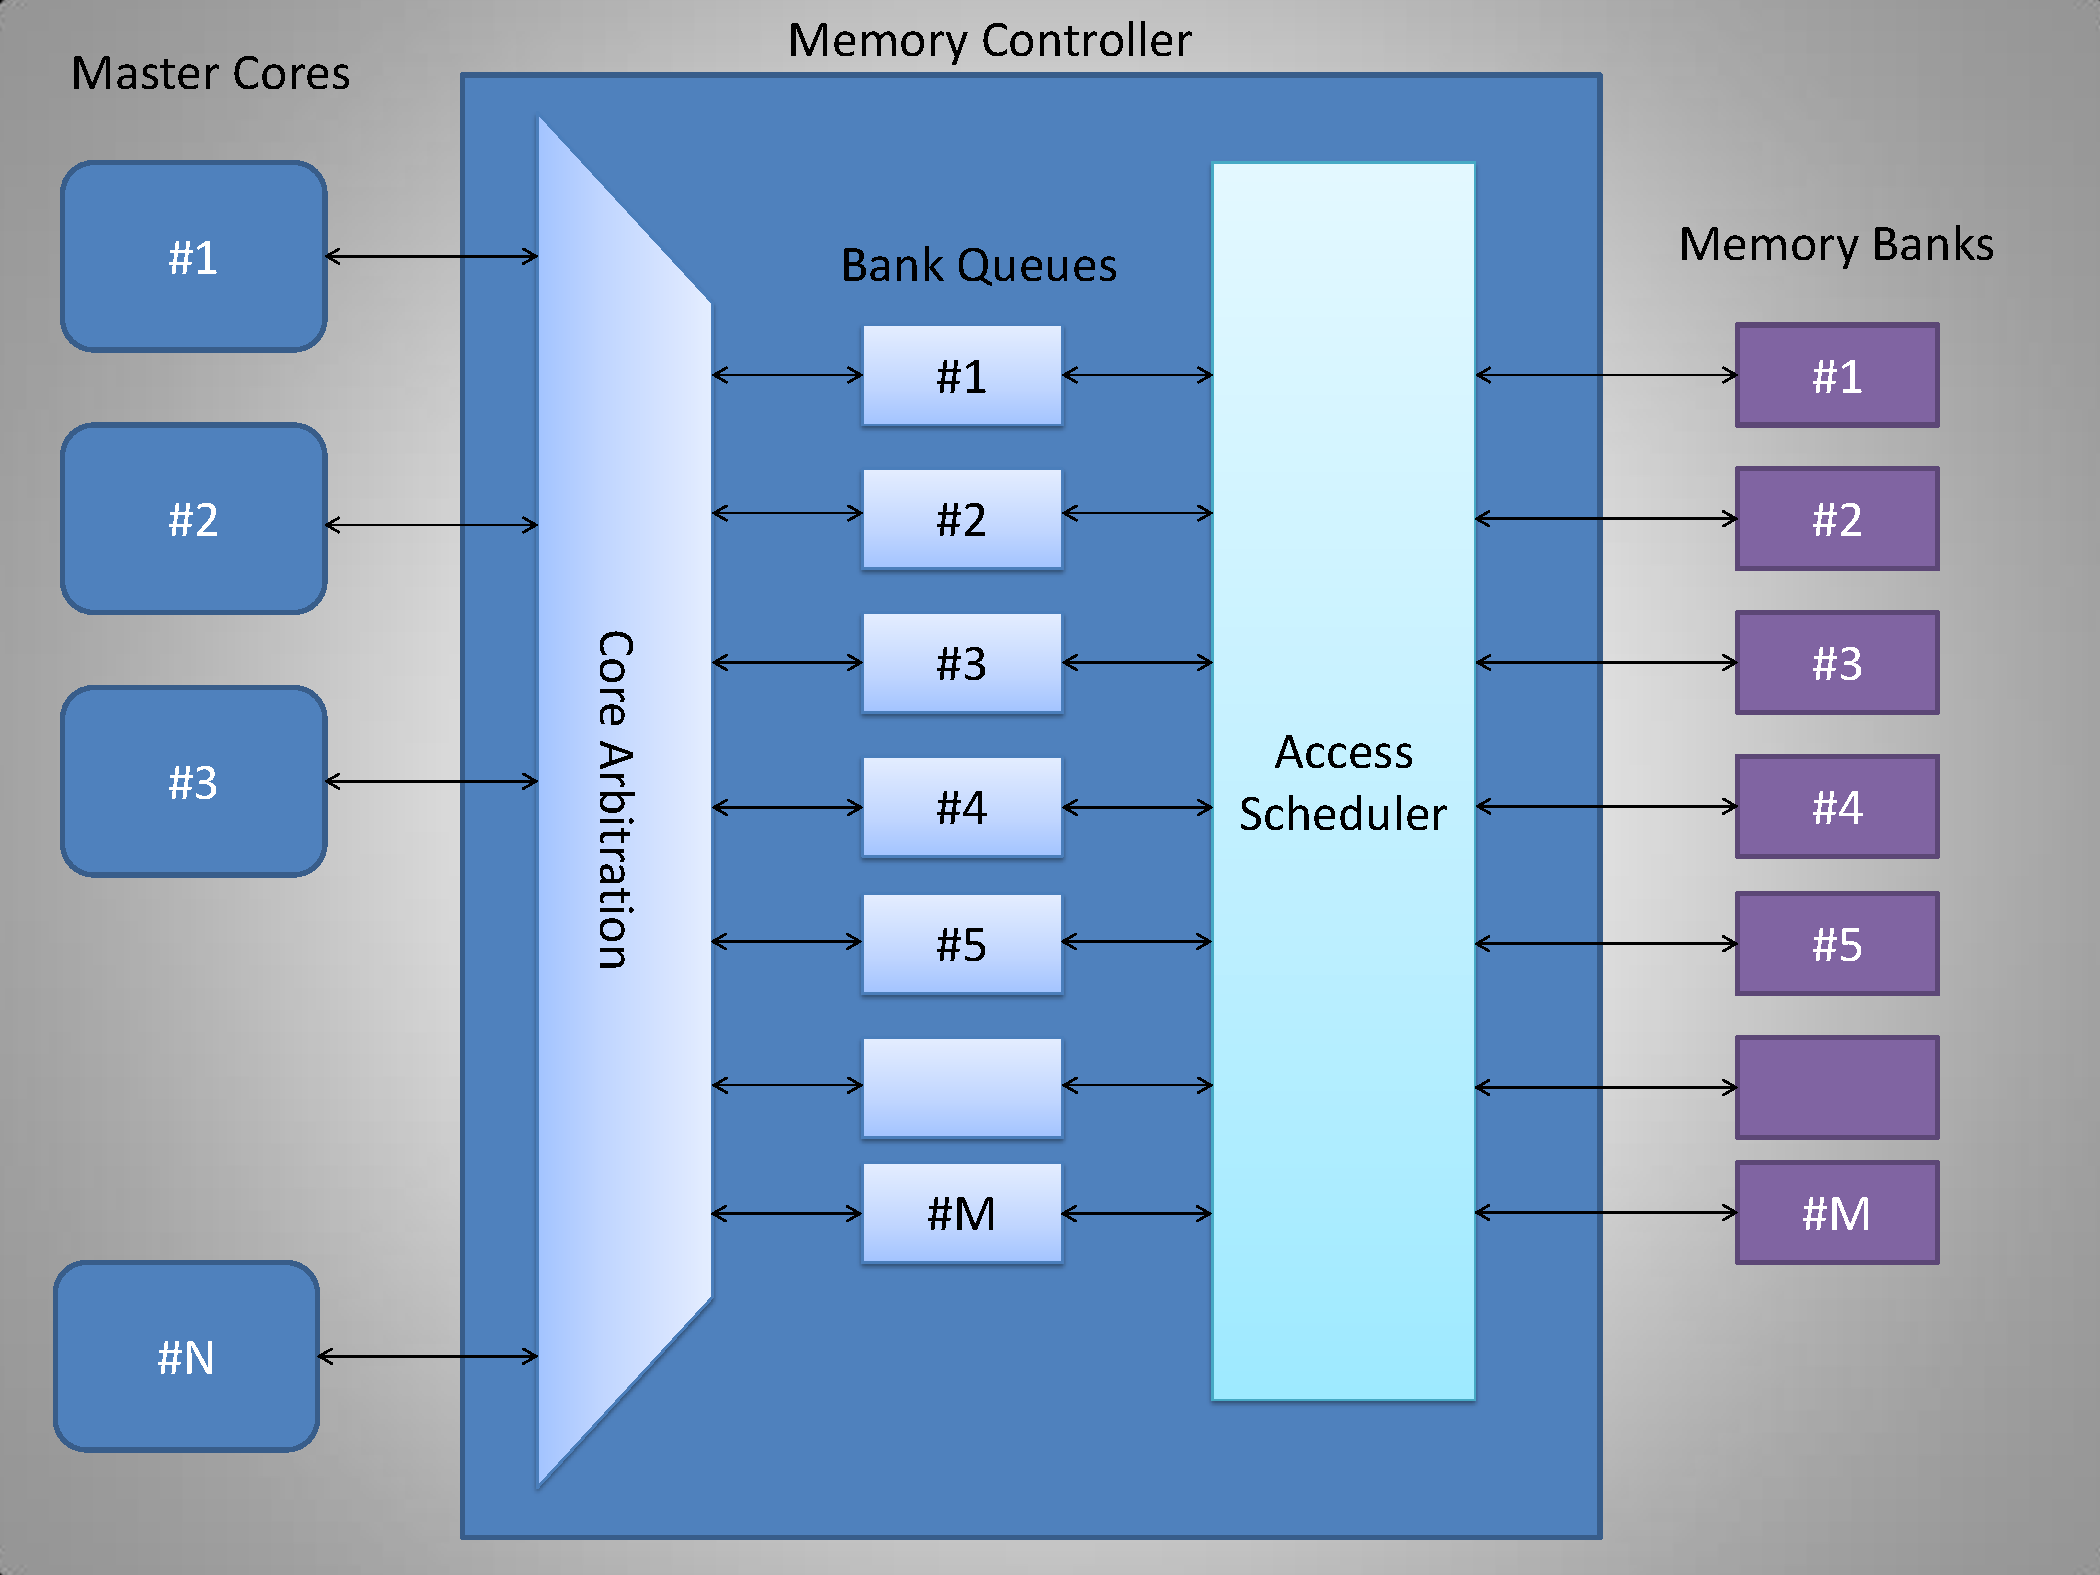
\includegraphics[width=0.7\linewidth]{fig/controllerArchitecture.pdf}
% \caption{
% {Architecture of Memory Controller} }
% \label{fig:pseudo-code}
% \end{figure}
% %-------------------------
The following three stages are illustrated in Figure~\ref{fig:multicore_arch}:
\begin{itemize}
\item \textbf{Core arbiter:~}Every clock cycle, the \textit{core arbiter} receives up to one request from each core which it stores in an internal queue. The core arbiter attempts to push these request to the appropriate bank queue. If it detects that the destination bank queue is full, the controller signals that the core is busy which stalls the core. The core arbiter also arranges the requests stored in its internal queue using a two-step priority order mechanism: first by Quality of Service (QoS) and then breaking ties with round-robin scheduling.

\item \textbf{Bank queues:~}Each data bank has a corresponding \textit{read queue} and \textit{write queue}.  The core arbiter sends memory requests to the bank queues until the queues are full. In our simulations, we use a bank queue depth of 10. There is also an additional queue which holds special requests such as memory refresh requests.

\item \textbf{Access scheduler:~}Every memory cycle, the \textit{access scheduler} chooses to serve read requests or write requests, algorithmically determining which requests in the bank queues it will schedule. The scheduling algorithms the access scheduler uses are called pattern builders. Depending on the current memory cycle's request type, the access scheduler invokes either the read or write pattern builder. A key design trade-off of the pattern builder algorithms is the relationship between the complexity of the algorithm and the number of requests the algorithm schedules.
\end{itemize}

We note that the core arbiter and bank queues should not differ much from those in a traditional uncoded memory controller. The access scheduler directly interacts with the memory banks, and therefore must be designed specifically for our coding schemes.


%-----------------------
\begin{figure}[tbp]
\centering
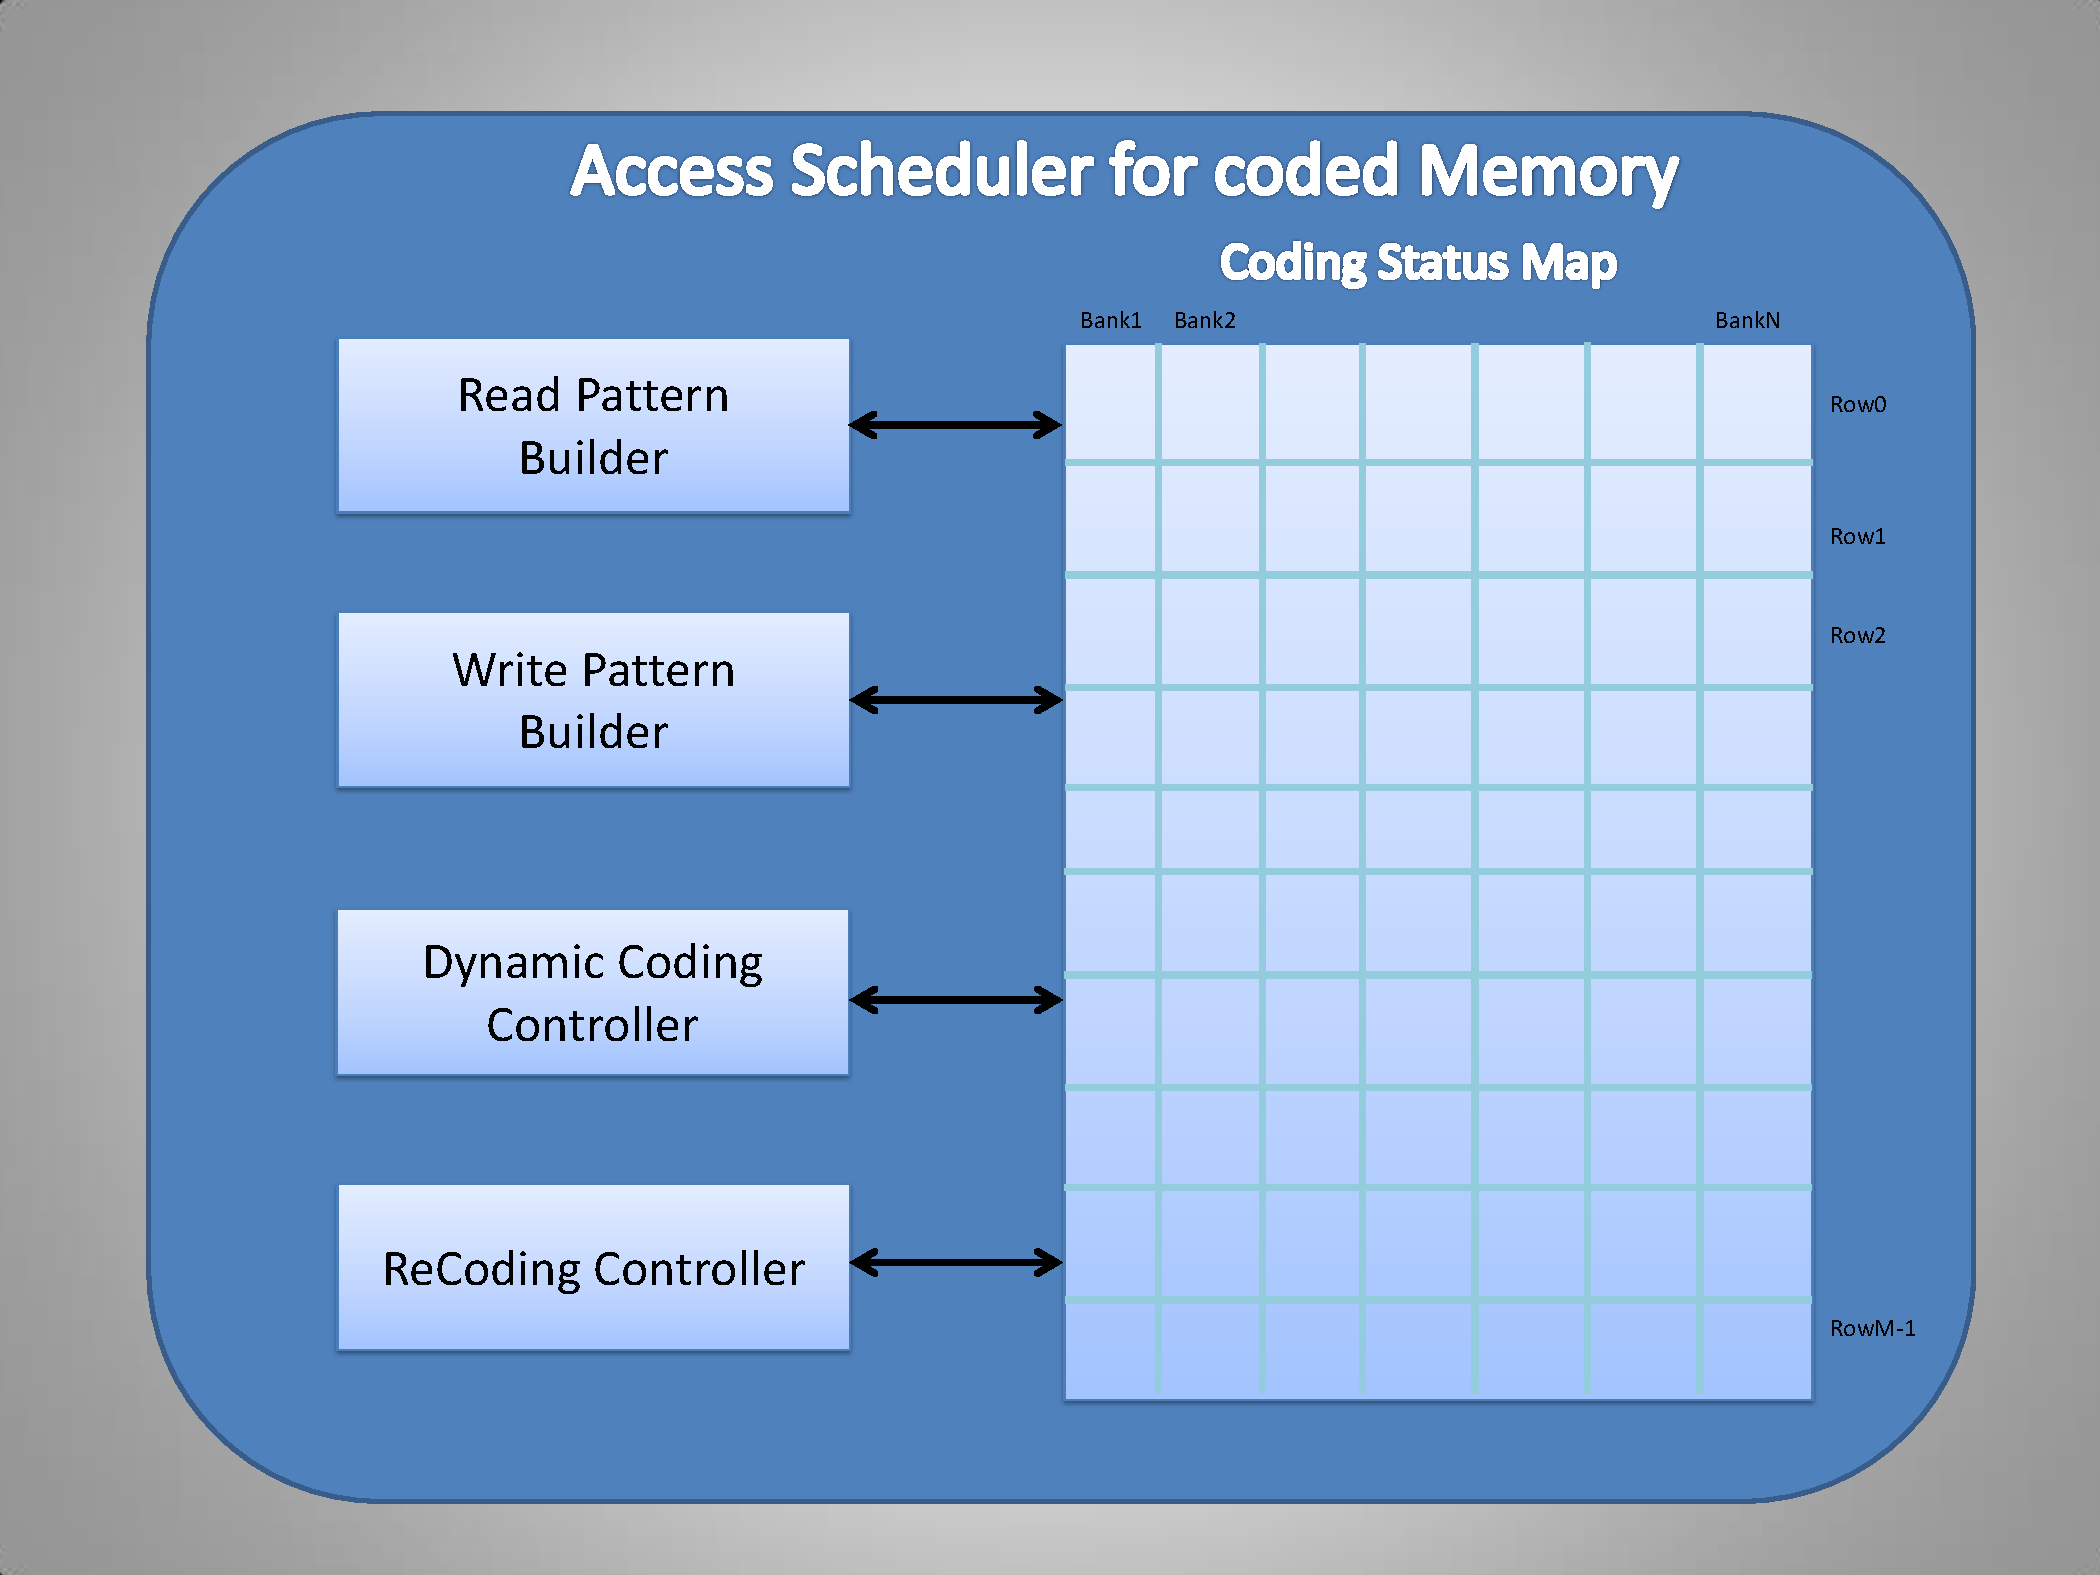
\includegraphics[width=0.7\linewidth]{fig/coded_access_scheduler.pdf}
\caption{
{Access scheduler for coded memory} }
\label{fig:coded_access_scheduler}
\end{figure}
%-------------------------
\subsection{Code Status Table}
\label{sec:codeStatusTable}
The code status table keeps track of the validity of data stored the data and parity banks. When a write is served to a row in a data bank, any parity bank which is constructed from the data bank will contain invalid data its corresponding row. Similarly, when the access scheduler serves a write to a parity bank, both the data bank which contains the memory address specified by the write request and any parity banks which utilizes that data bank will contain invalid data. The code status table keeps track of the locations of invalid data so the access scheduler does not erroneously serve read requests with stale data.

Figure~\ref{fig:coded_access_scheduler} depicts our implementation of the code status table. It contains an entry for every row in each data bank, which can take one of three values indicating 1) the data in both the data bank and parity banks is fresh, 2) the data bank contains the most recent data, or 3) one of the parity banks contains the most recent data. 
%It is not necessary for the code status table to know which parity bank a write request was served, because the dynamic coding unit described later in this section keeps track of this information. 
We assume that the elements of the code status table are accessible at a very fast rate. 


%{\color{red}
%This implementation of the code status table can be improved. This code status table does not keep track of the intermediate steps the access scheduler takes when rebuilding codes after a write is served. When rebuilding the memory in two parity banks after a data bank has been written to, it is likely that elements of one parity bank will be restored before the other. The restored parity bank is ready to serve more memory requests using the rebuilt row, but the code status table will indicate that all the parity banks are unavailable until all parity banks are restored. Full knowledge of the status of all data and parity banks allows the access scheduler to serve more requests in some scenarios. \Matt{is this example necessary? Is the tangent worth the insight?}
%}

%-----------------------
\begin{figure}[t!]
	%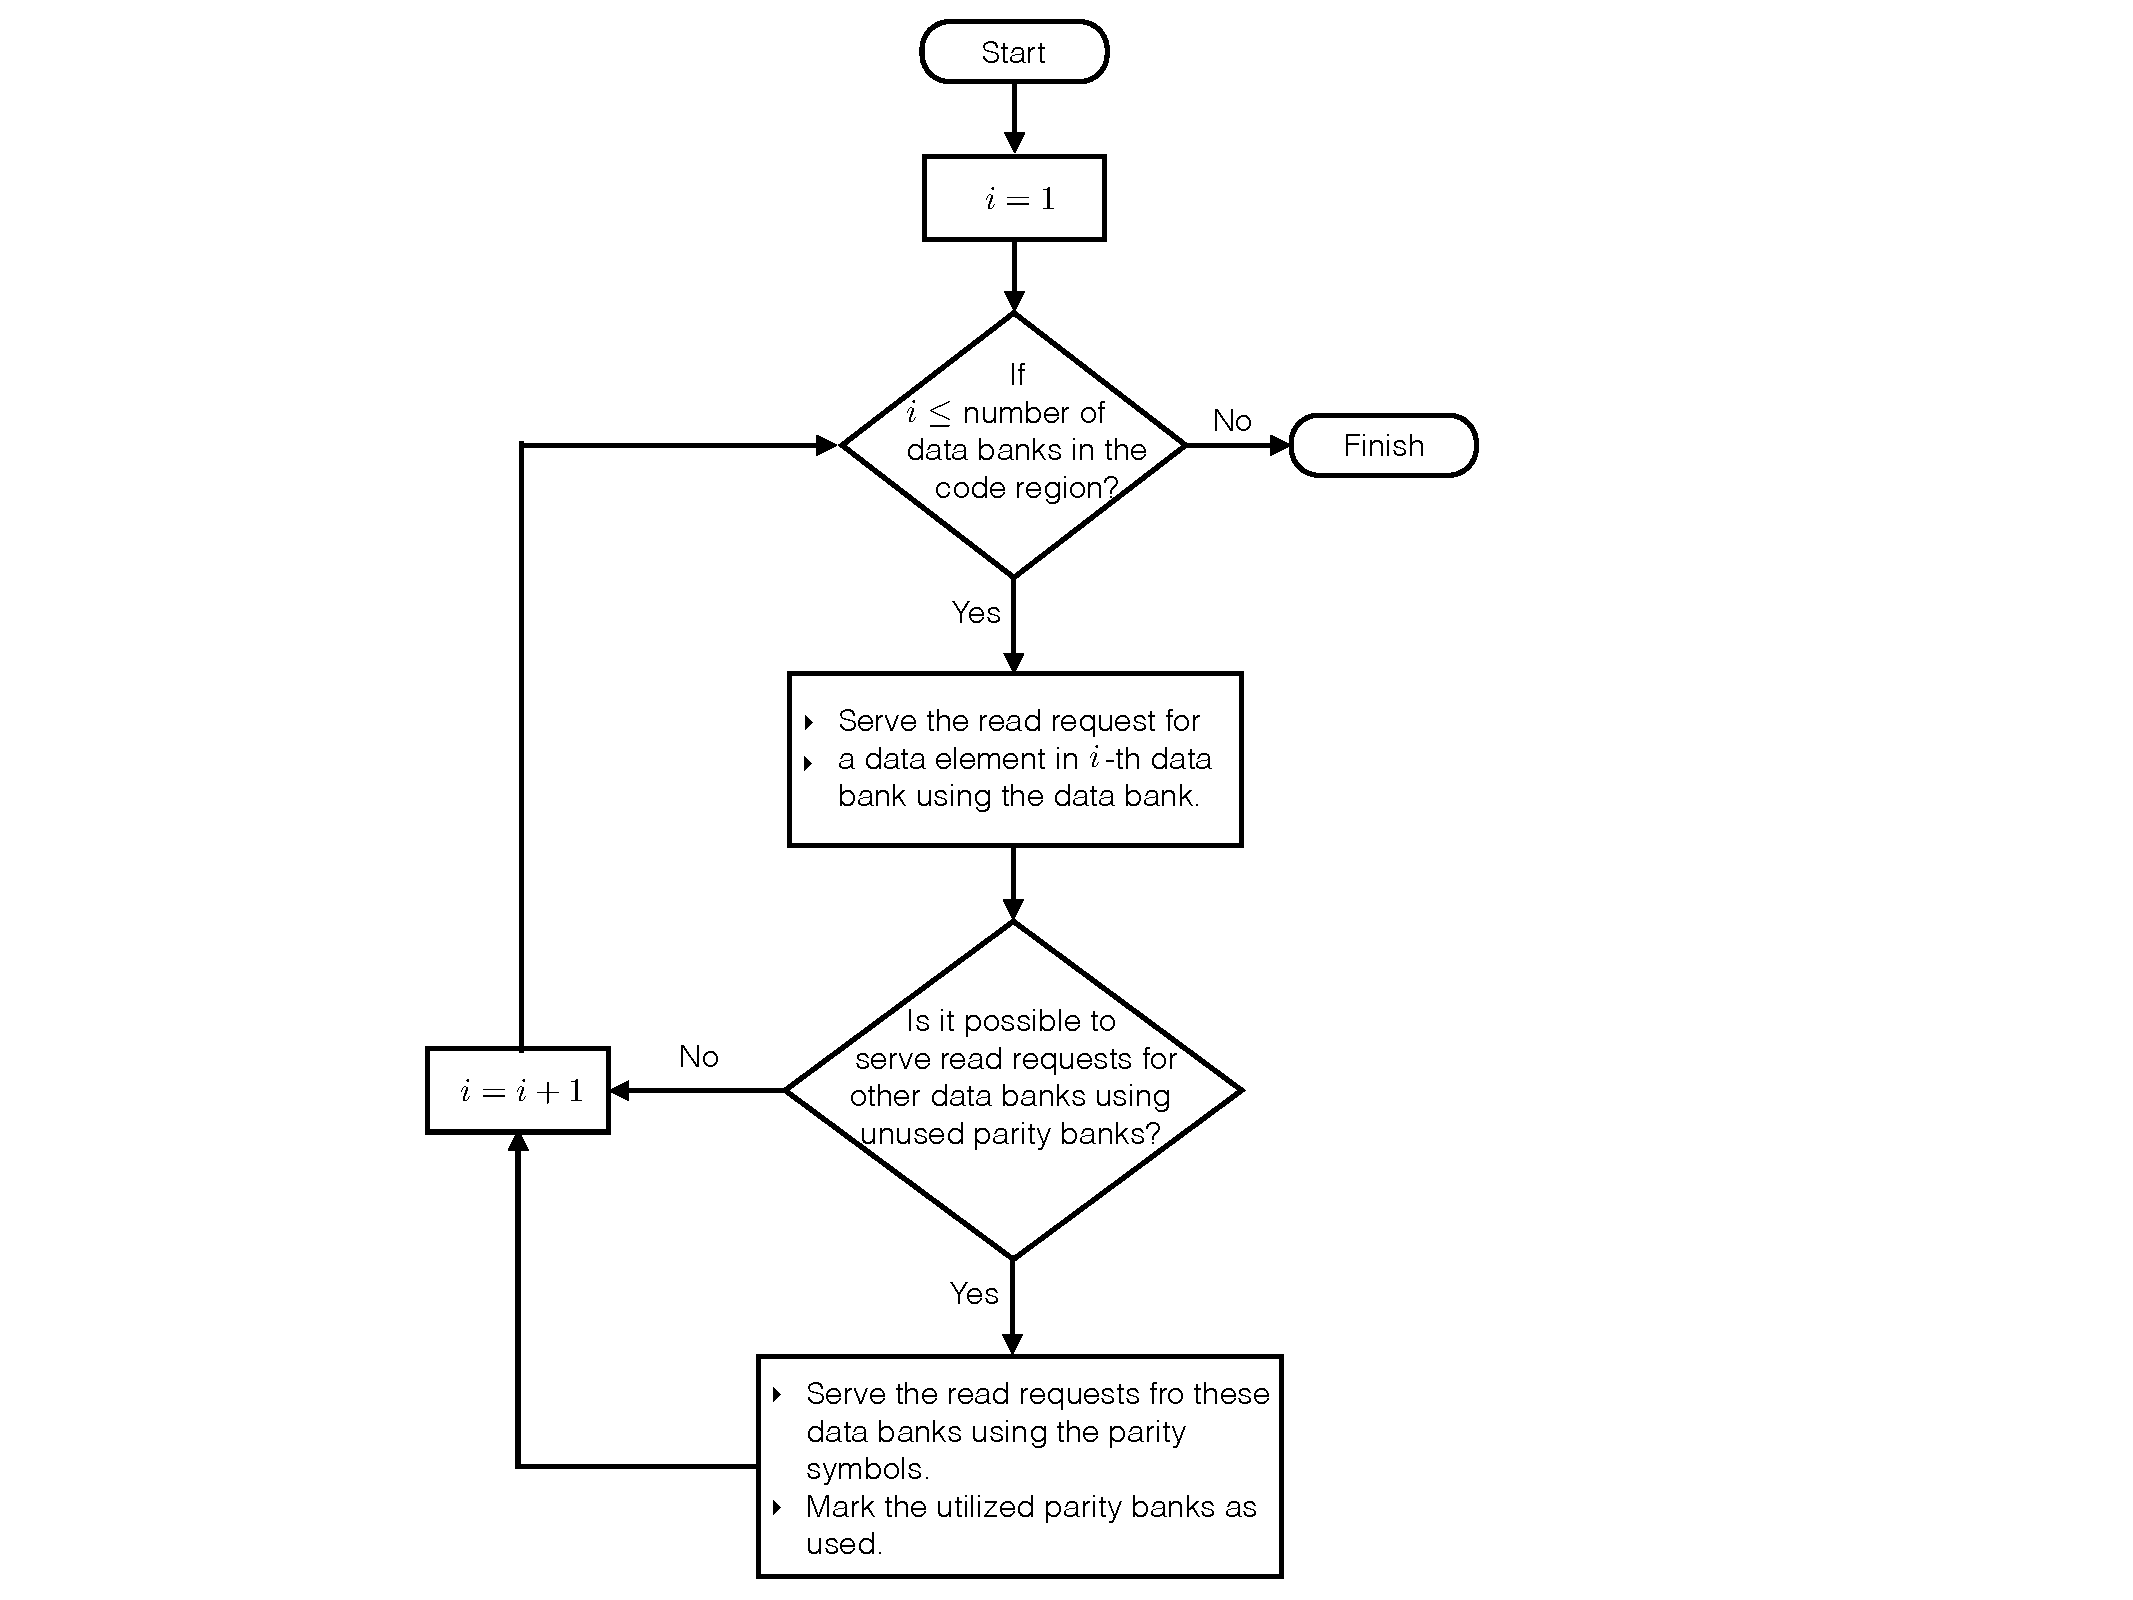
\includegraphics[width=0.9\linewidth]{fig/Read-algo.pdf}
	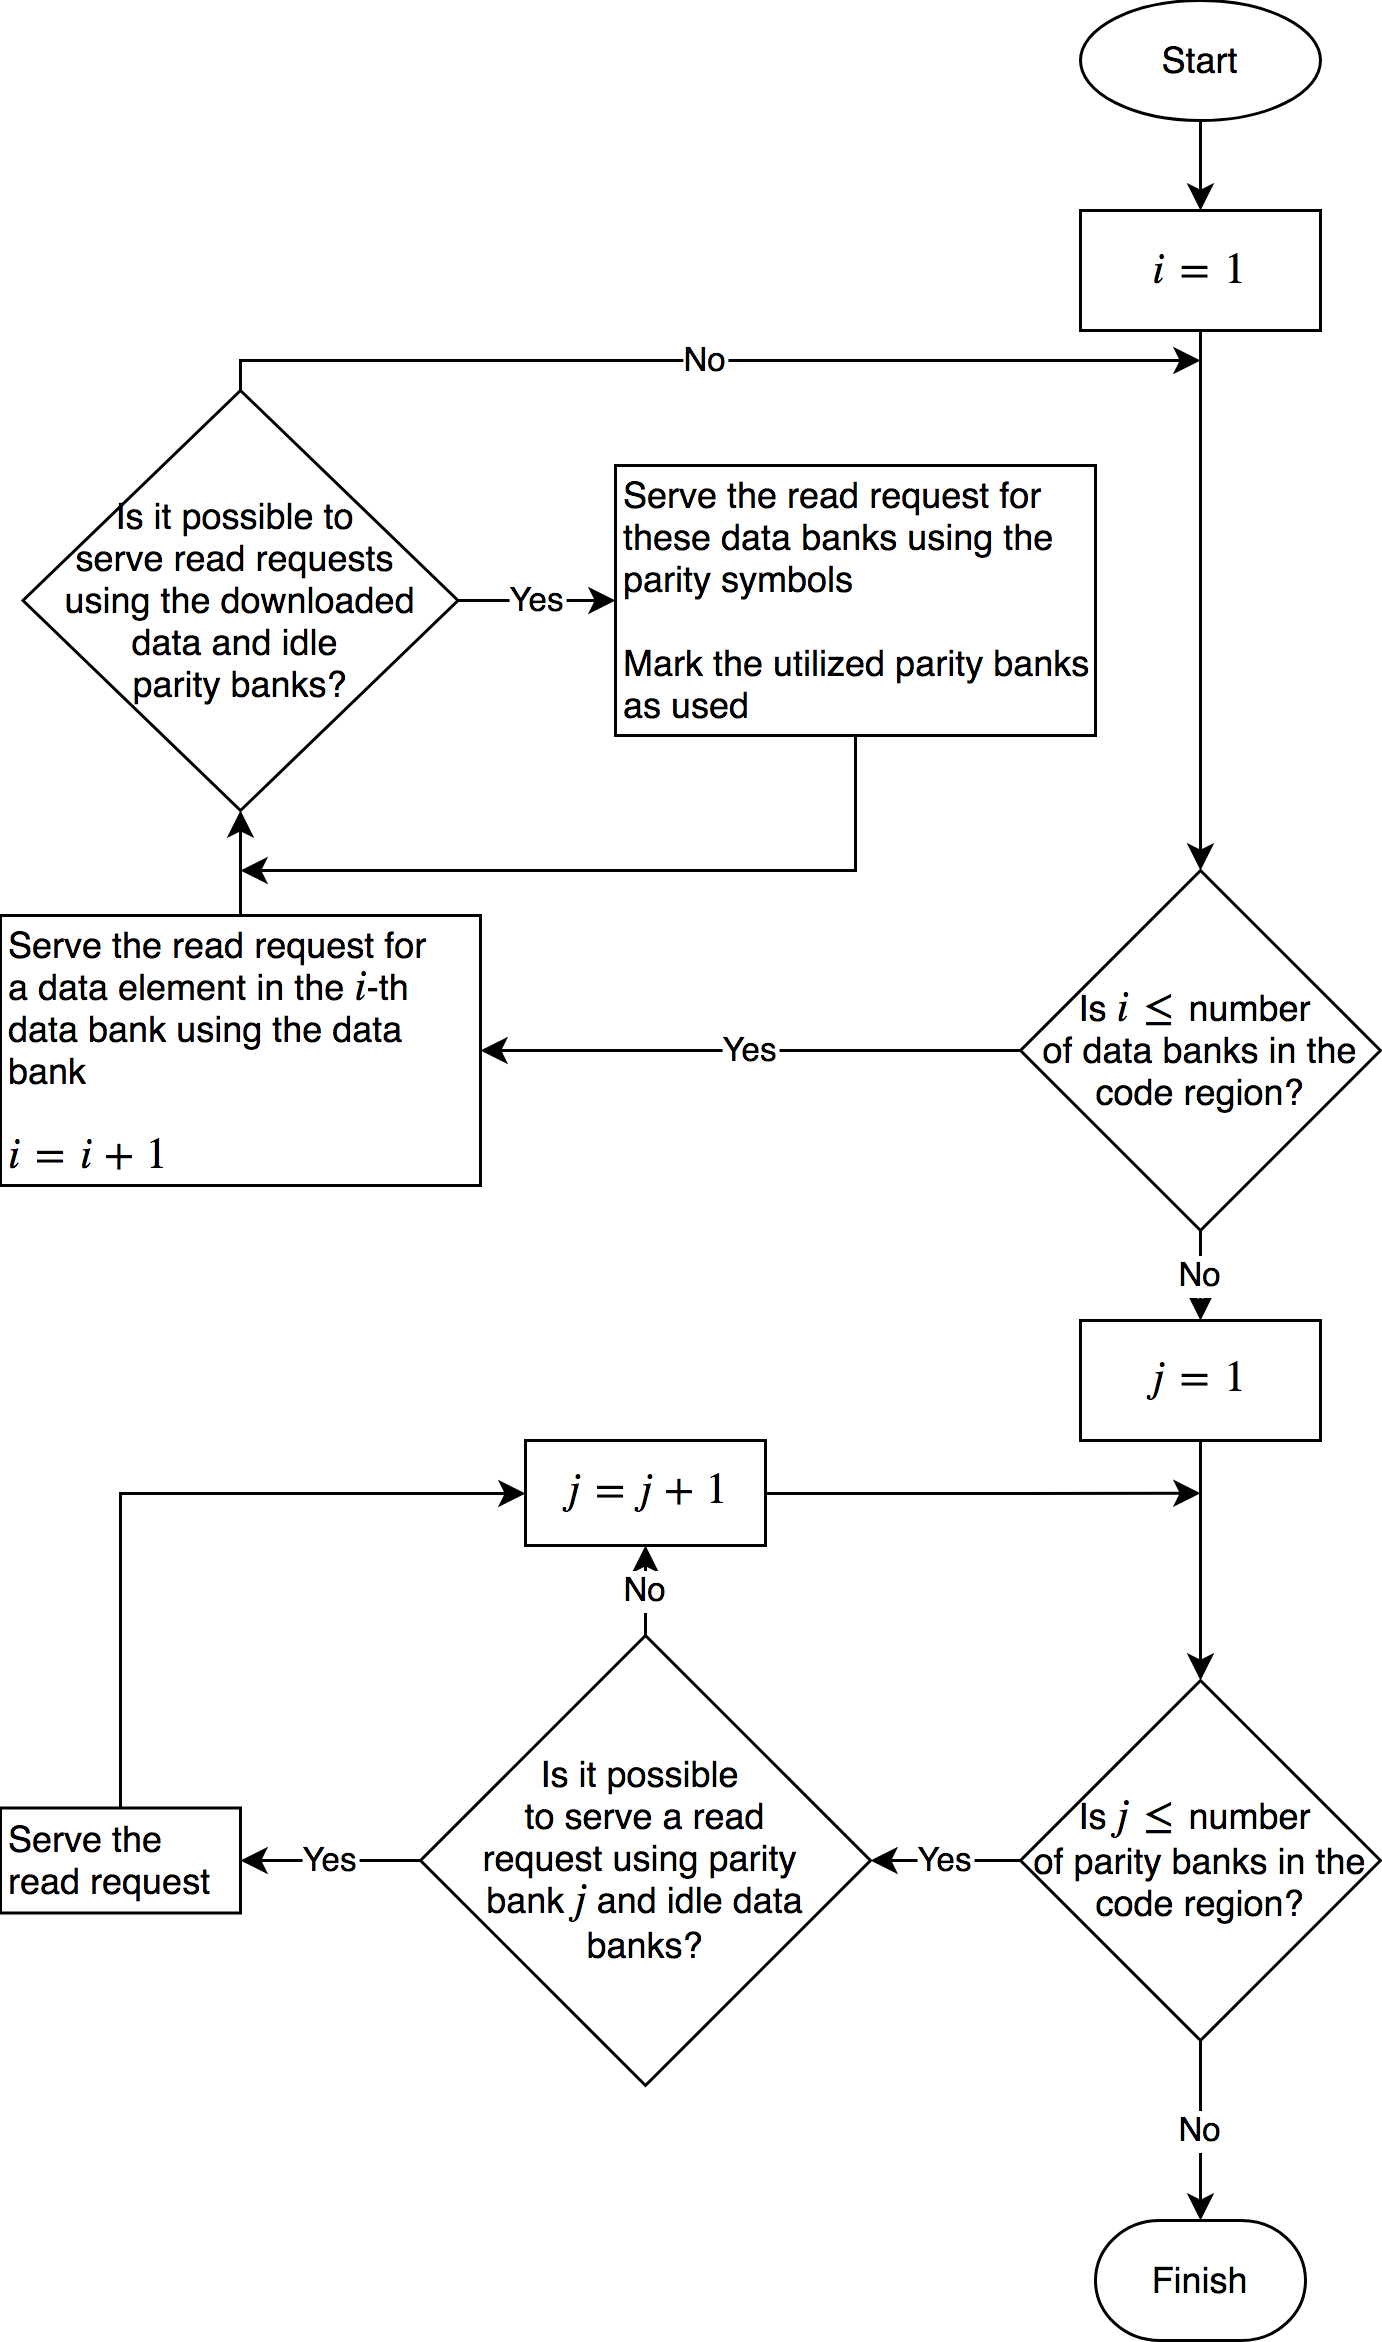
\includegraphics[width=0.96\linewidth]{fig/read_pattern_algo.png}
	\caption{{Description of the algorithm to build a read request pattern to be served in a given memory cycle.}}
	\label{fig:readAlgo}
\end{figure}
%-------------------------
%-----------------------
\begin{figure}[htbp]
	\centering
	%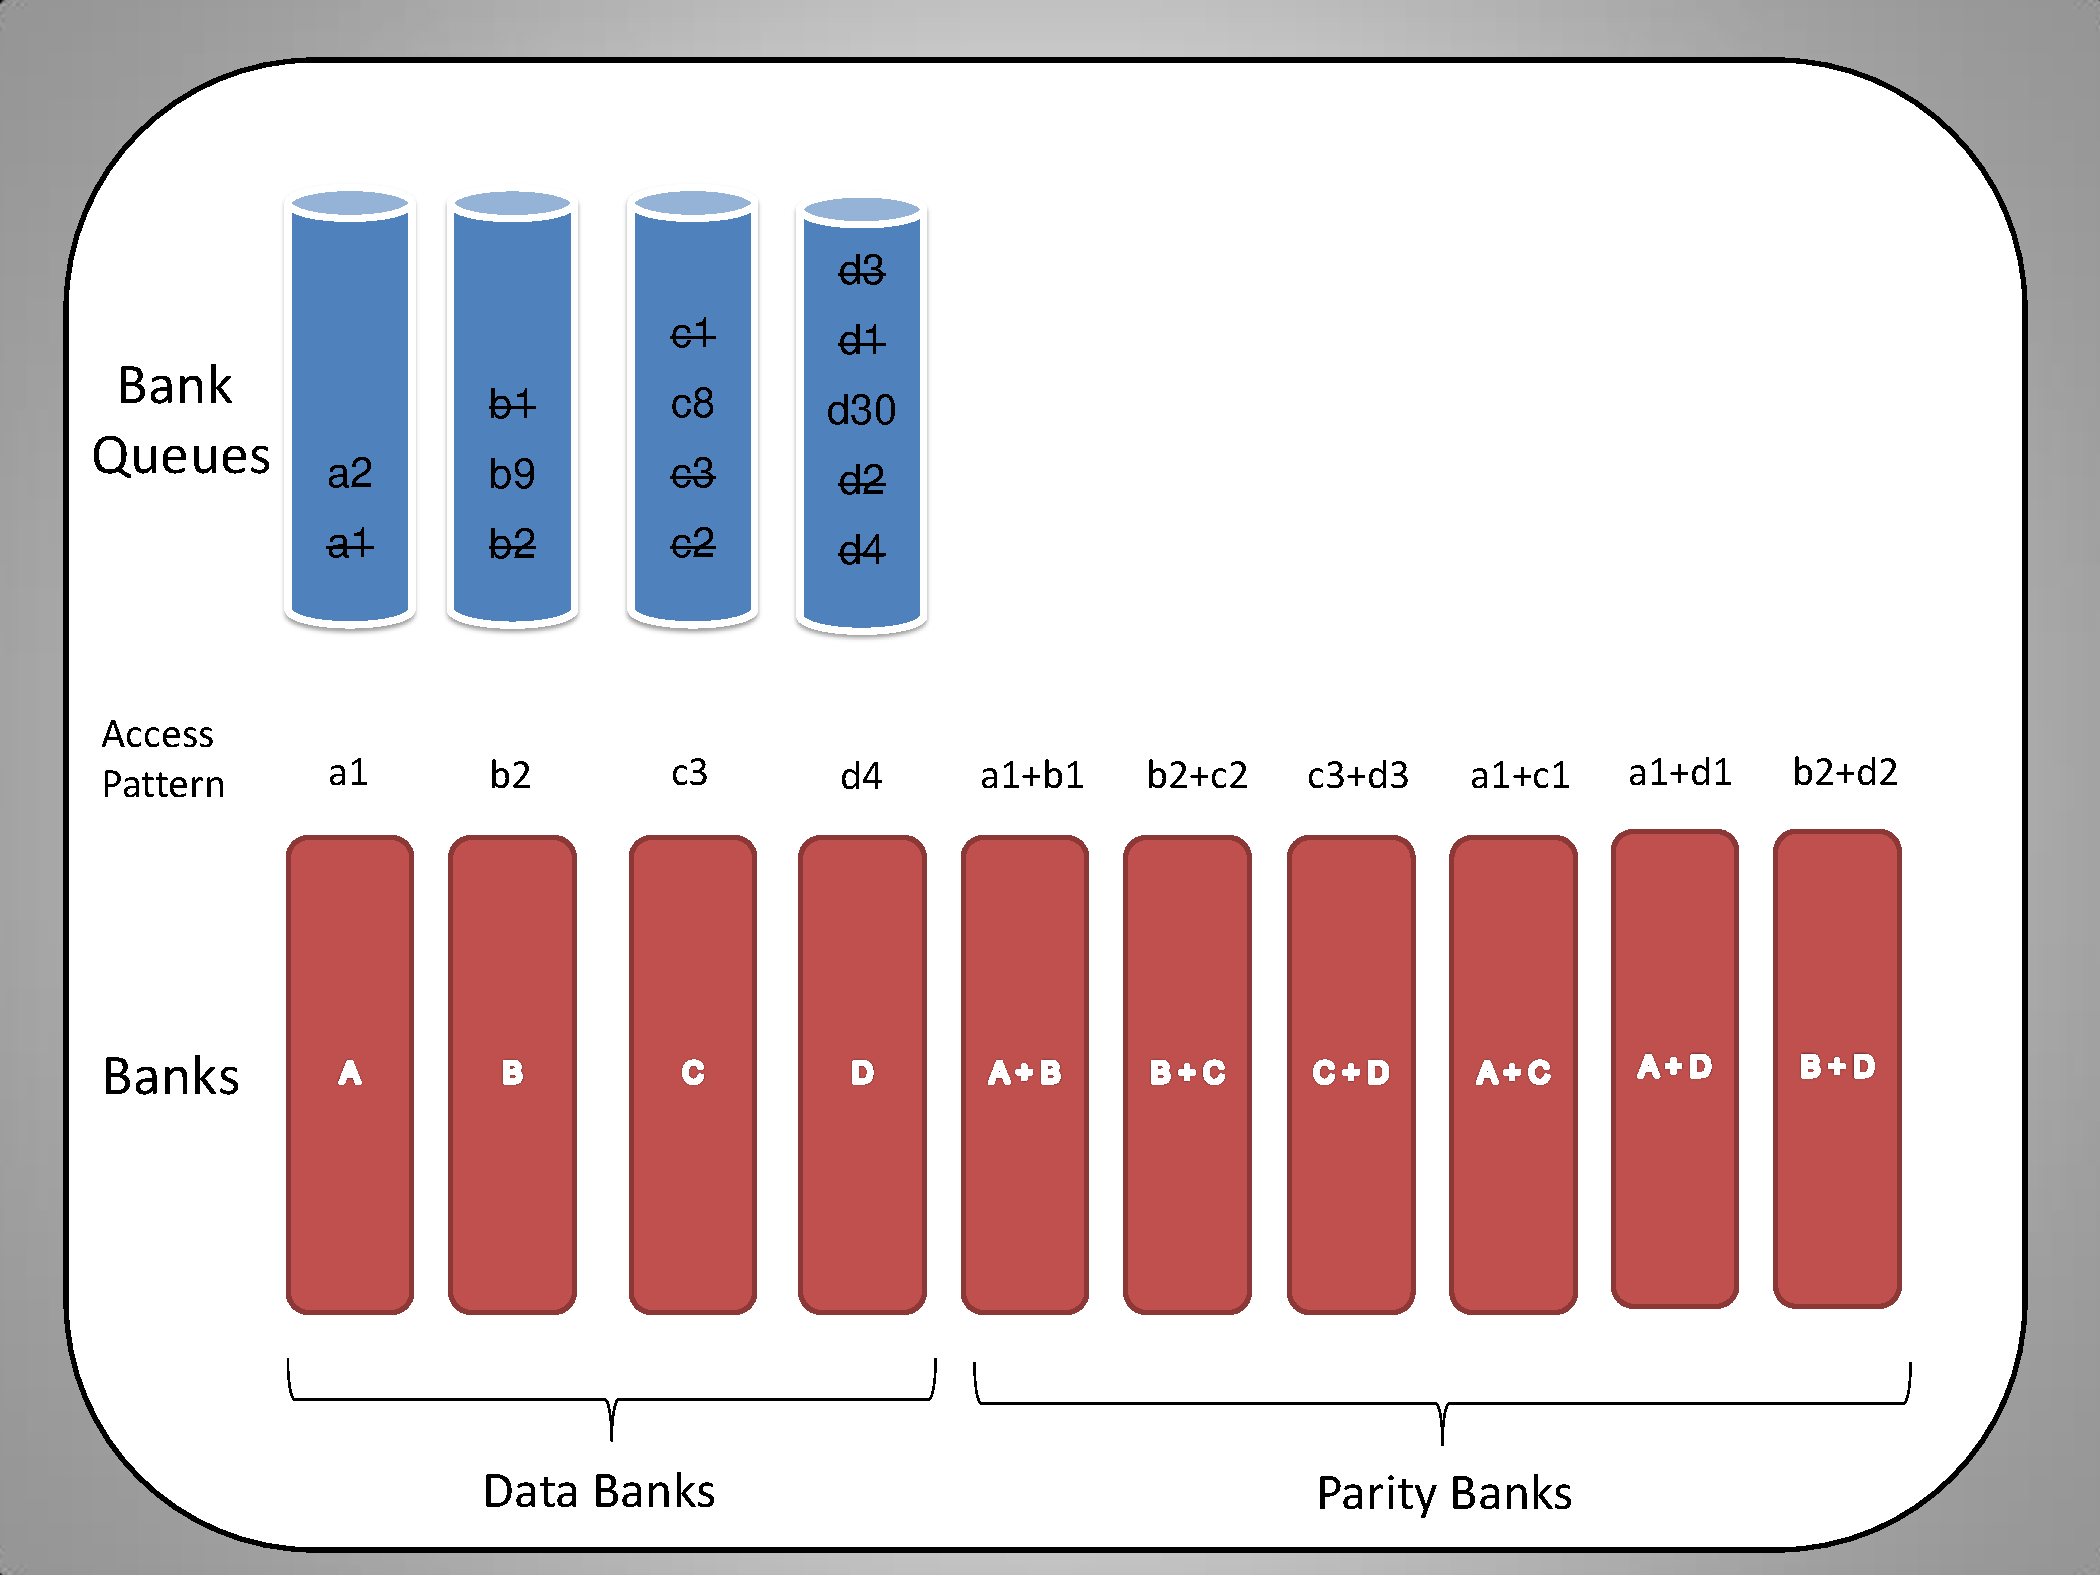
\includegraphics[width=0.7\linewidth]{fig/readAlgoAccessPattern.pdf}
	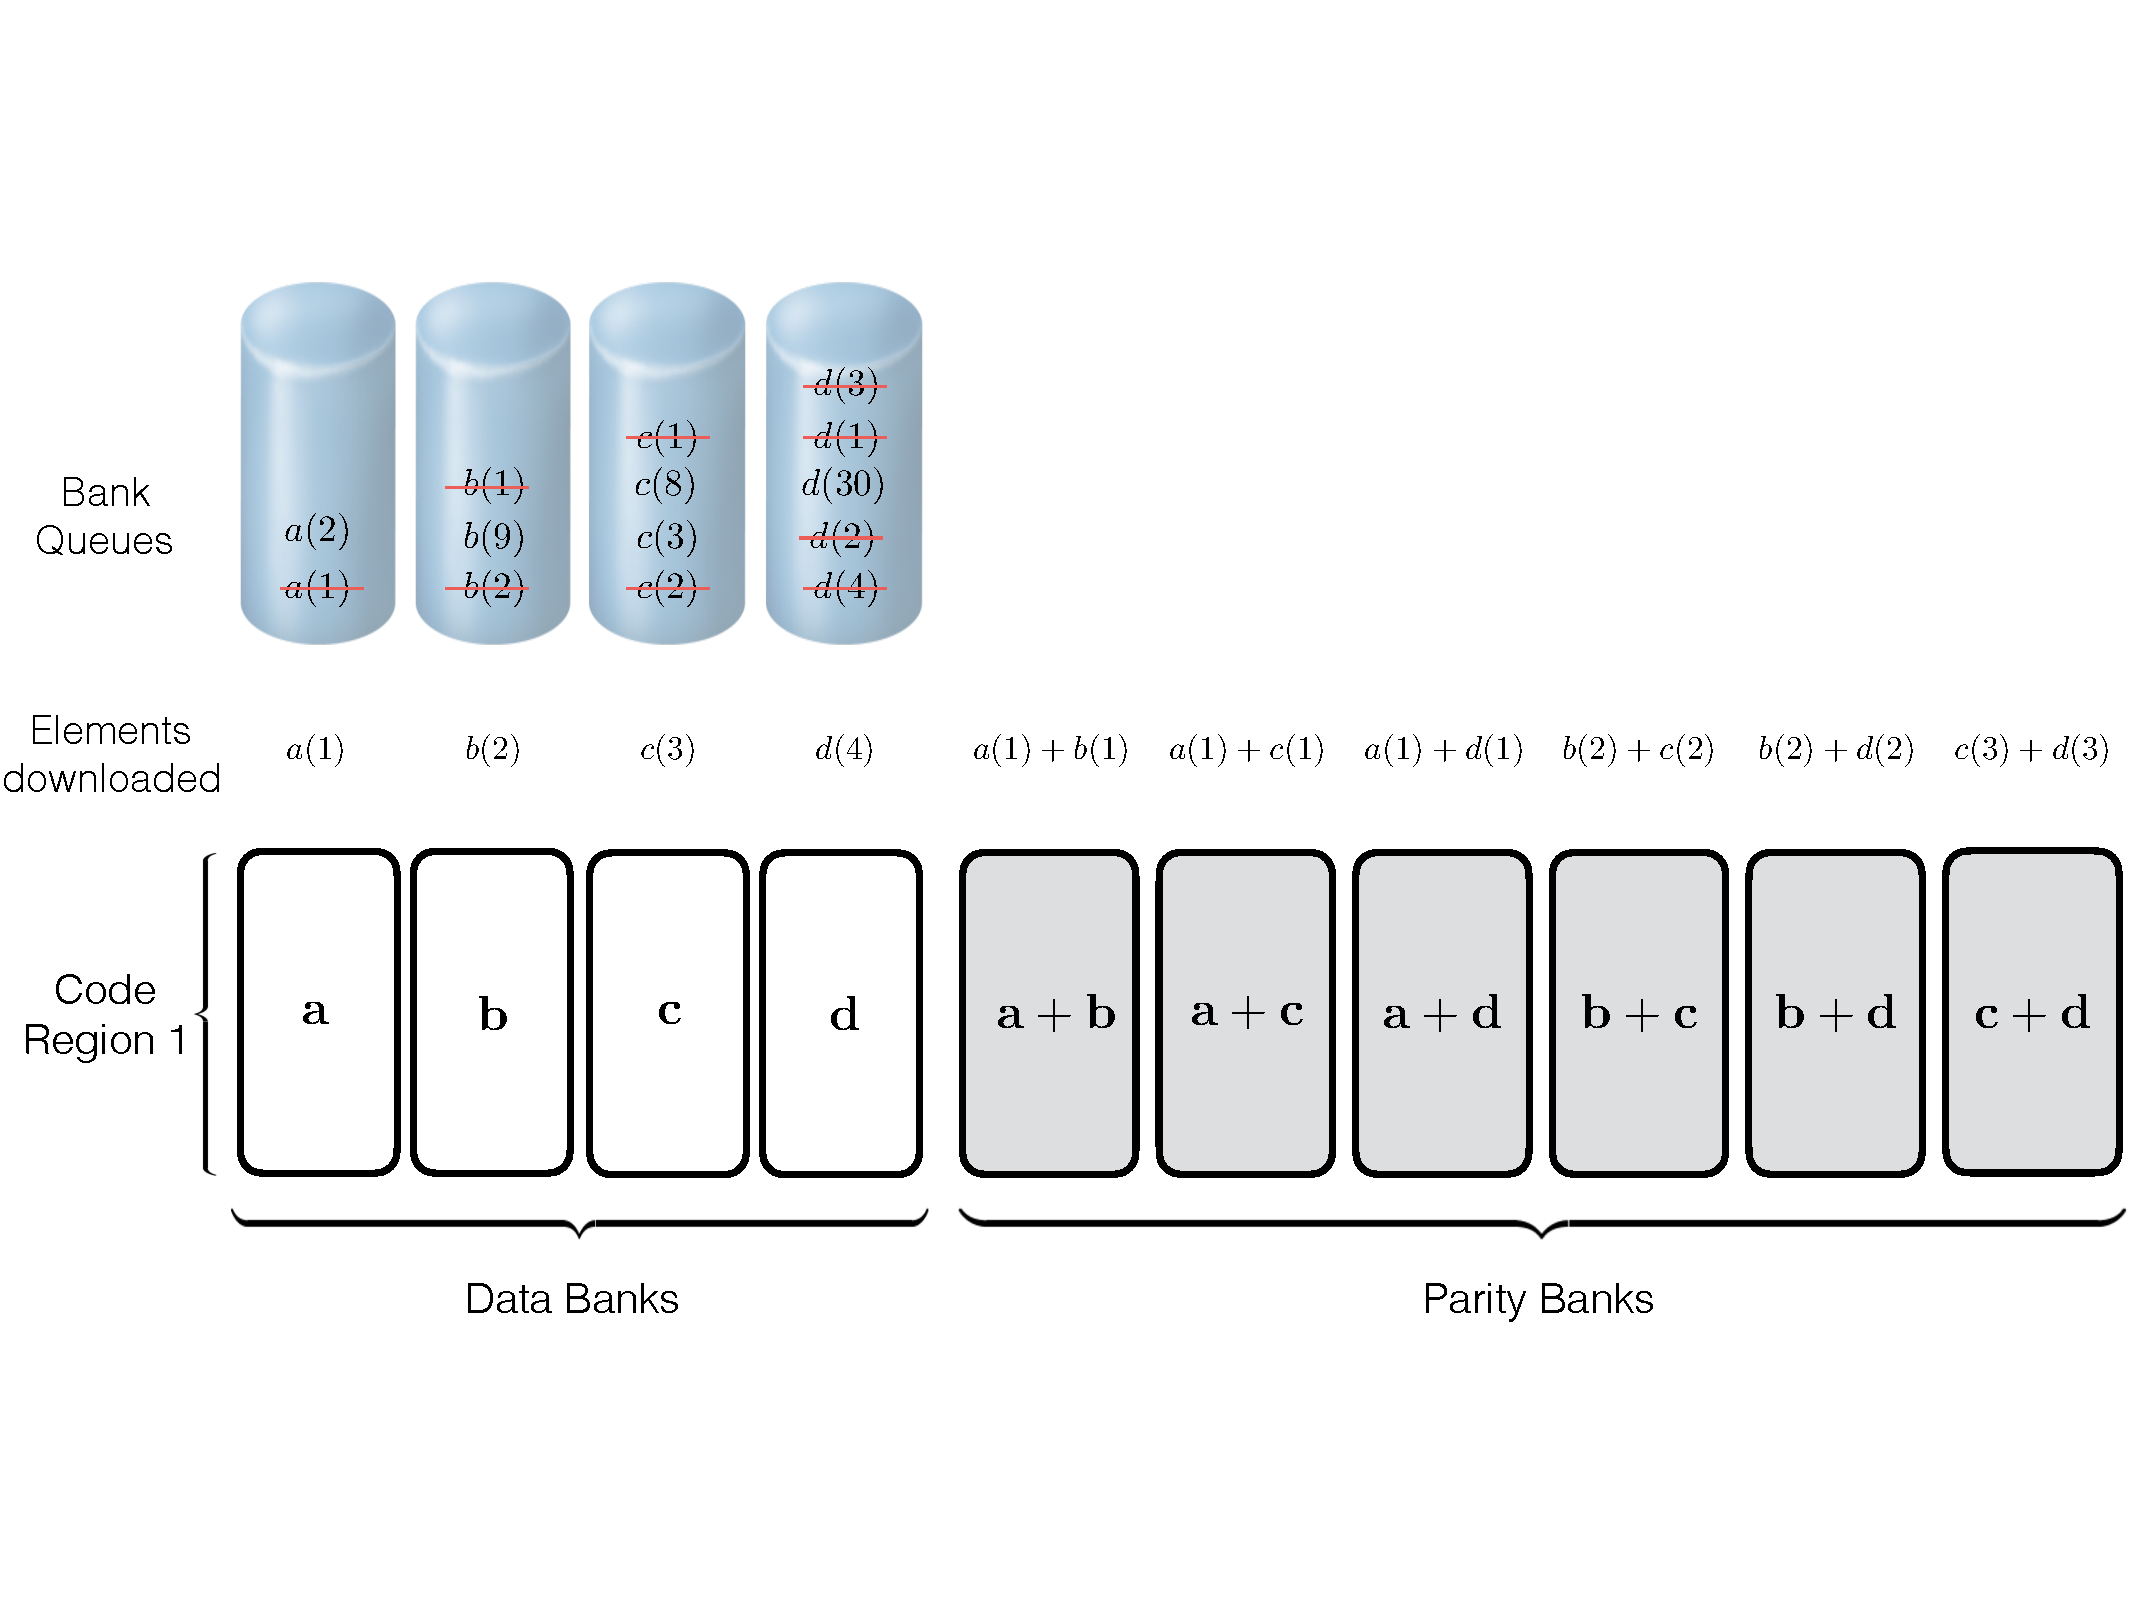
\includegraphics[width=0.96\linewidth]{fig/Read-Algo-Example.pdf}
	\caption{{Illustration of the algorithm to build a read request pattern to be served in a given memory cycle. All the read requests associated with the strikethrough elements are scheduled to be served in a given memory cycle. The figure also shows the elements downloaded from all the memory banks in order to serve these read requests.}}
	\label{fig:readAlgoAccessPattern}
\end{figure}
%------------------------
%\subsection{Read Algorithm for Coded Memory system}
\subsection{Read pattern builder}
\label{sec:readCodingAlgo}


The access scheduler uses the read pattern builder algorithm to determine which requests to serve using parity and which to use data banks. The read pattern builder selects which memory requests to serve and determines how requests served by parity banks will be decoded. The algorithm is designed to serve many read requests in a single memory cycle. Figure~\ref{fig:readAlgo} shows our implementation of the read pattern builder.

Figure~\ref{fig:readAlgoAccessPattern} shows an example read pattern constructed by our algorithm. First, $a(1)$ is marked to be read from data bank $\mathbf{a}$. Then the algorithm looks through banks $\mathbf{b}$, $\mathbf{c}$, and $\mathbf{d}$ for requests for rows $b(1)$, $c(1)$, or $d(1)$ because these symbols can be decoded from a parity bank using the $a(1)$ symbol. In this scenario all three are present in the bank queues and are served using parity banks. Symbols equal to  $a(1) + b(1)$, $a(1) + c(1)$, and $a(1) + d(1)$ are all downloaded from parity banks and decoded with $a(1)$. Next, $b(2$) is read from a data bank. Similar to before, $c(2)$ and $d(2)$ are served by downloading $b(2) + c(2)$ and $b(2) + d(2)$ symbols from the parity banks. Again as before, $c(3)$ is read from data bank and $d(3)$ is decoded using $c(3)$ and $c(3) + d(3)$. Finally, $d(4)$ is read from a data bank.

\begin{remark}
By increasing the number of read requests per cycle, we increase the risk of having out-of-order execution of memory access requests on the same core. We assume that the code arbiter only admits requests into the bank queues if they can be immediately served without introducing harmful out-of-order execution.


\end{remark}
\ignore{
%-----------------------
\begin{figure}[htbp]
\centering
	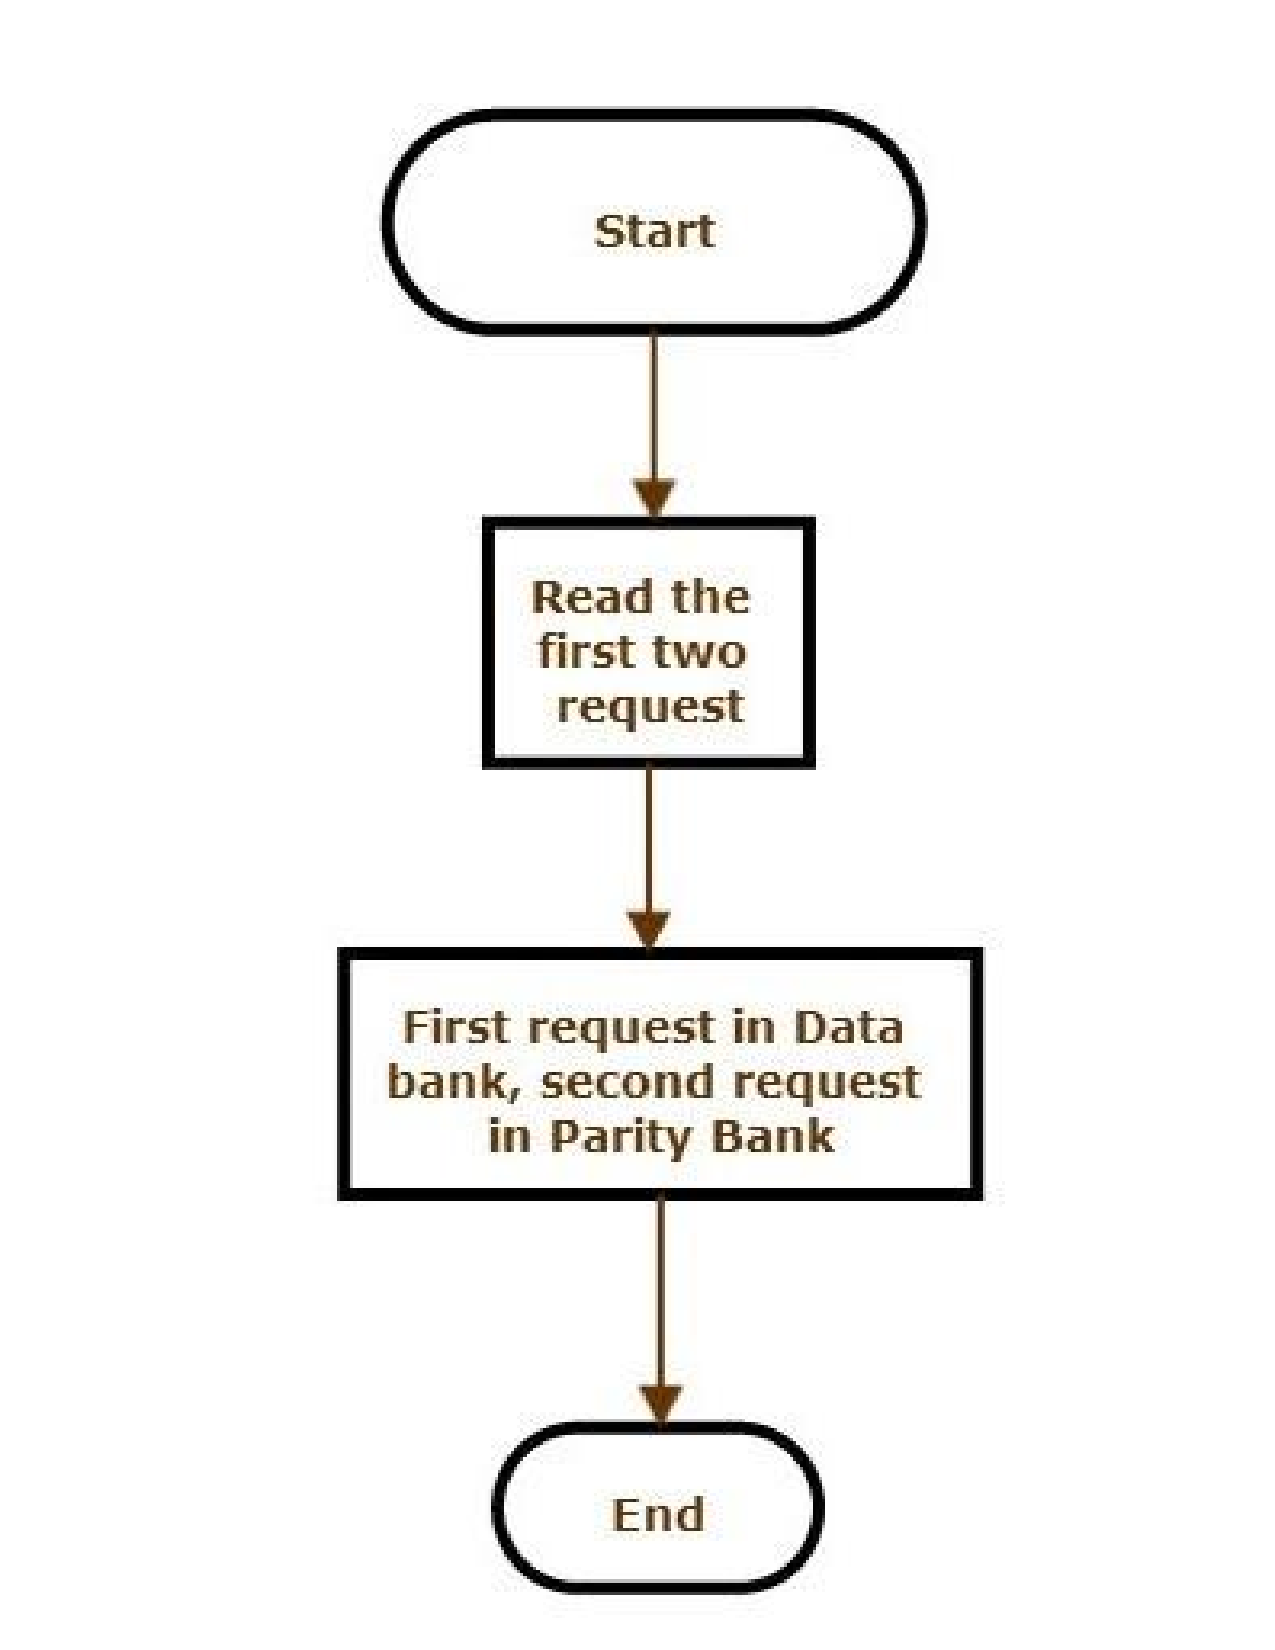
\includegraphics[width=\linewidth]{fig/writealgo.pdf}
	\caption{{\bf Flowchart of Write Algorithm}}
	\label{fig:writeAlgo}
\end{figure}
%-------------------------
%\ignore{
\begin{itemize}
\item Write about how we solve the out of order look ahead problem. If we solve 
	it at all ????
\end{itemize}
}
%\subsection{Write Algorithm for Coded Memory system}
\subsection{Write pattern builder}
\label{sec:writeCodingAlgo}
Parity banks allow the memory controller to serve additional write requests per cycle. When multiple writes target a single bank, it can commit some of them to parity banks. The access scheduler implements a write pattern builder algorithm to determine which write requests to schedule in a single memory cycle. Figure~\ref{fig:writeFlow} illustrates our implementation of the write pattern builder. Only when the write bank queues are nearly full does the access scheduler execute the write pattern builder algorithm. 


%-----------------------
\begin{figure}[htbp]
\centering
	\includegraphics[width=\linewidth]{fig/write_pattern_algo.png}
	\caption{{ Flowchart of write pattern builder}}
	\label{fig:writeFlow}
\end{figure}
%-------------------------


Figure~\ref{fig:writeAlgoAccessPattern} shows an example write pattern produced by our algorithm. Parity banks increase the maximum number of write requests from $4$ to $10$. Note that an element which is addressed to row $n$ in a data bank can only be written to the corresponding row $n$ in the parity banks. In this scenario, the write queues for every data bank are full. The controller takes $2$ write requests from each queue and schedules one to the queue's target data bank and the other to a parity bank. The controller also updates the code status table.

{\color{red}
Figure~\ref{fig:writeAlgoAccessPattern} also demonstrates how the code status table changes to reflect the freshness of the elements in the data and parity banks. Here, the 00 status indicates that all elements are updated. The 01 status indicates that the data banks contain fresh elements and the elements in the parity banks must be recoded. The 10 status indicates that the parity banks contain fresh elements, and that both data banks and parity banks must be updated.
}

%-----------------------
\begin{figure}[t!]
\centering
         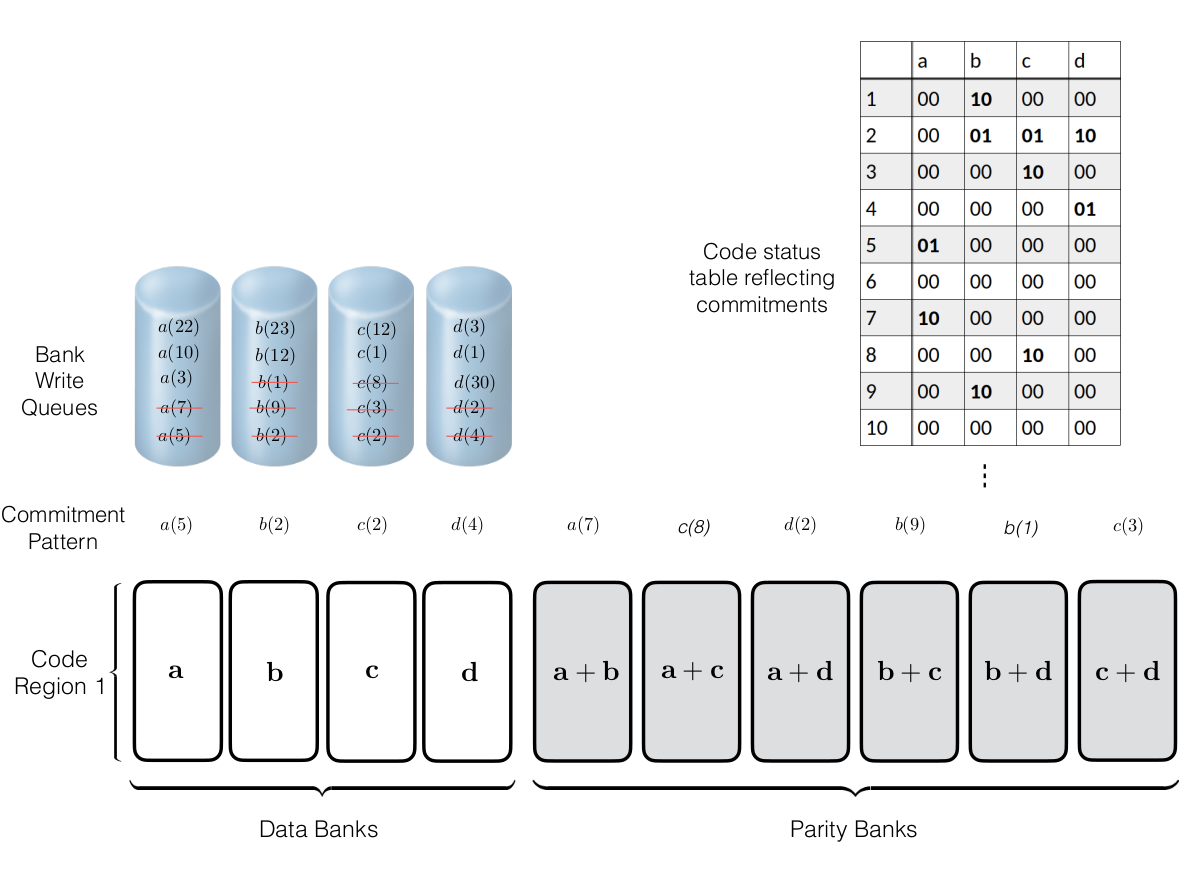
\includegraphics[width=\linewidth]{fig/Write-Algo-Example.png}
	\caption{The behavior of the write pattern builder on a 4-bank memory system}
	\label{fig:writeAlgoAccessPattern}
\end{figure}
%-------------------------
\subsection{ReCoding unit}
\label{sec:recoding}
After a write request has been served, the stale data in the parity (or data) banks must be replaced. The \textit{ReCoding Unit} accomplishes this with a queue of {\em recoding requests}. Every time a write is served, recoding requests are pushed on to the queue indicating which data and parity banks contain stale elements, as well as the bank which generated the recoding request. Requests also contain the current cycle number so that the ReCoding Unit may prioritize older requests. Appendix

\subsection{Dynamic Coding}
\label{sec:dynamicCoding}
To reduce memory overhead $\alpha$, parity banks are designed to be smaller than data banks. The dynamic coding block maintains codes for the most heavily accessed memory subregions, so that parity banks are utilized more often.
%
%\subsubsection{Encoder Design}
%There are many possible implementations of the dynamic coding unit. The design described here is used in the simulator used to generate the results described in sections 5 and 6.
%
The {\em dynamic coding} block partitions each memory bank into $\lceil\frac{1}{r}\rceil$ regions. The block can select up to $\frac{\alpha}{r} - 1$ regions to be encoded in the parity banks. A single region is reserved to allow encoding of a new region.

Every $T$ cycles, the dynamic coding unit chooses the $\frac{\alpha}{r} - 1$ regions with the greatest number of memory accesses. The dynamic coding unit will then encode these regions in the parity banks. If all the selected regions are already encoded, the unit does nothing. Otherwise, the unit begins encoding the most accessed region. Once the dynamic coding unit is finished encoding a new region, the region becomes available for use by the rest of the memory controller. A memory region of length $r$ is reserved by the dynamic coding unit for constructing new encoded regions, and a memory region of length $\alpha - r$ is reserved for active encoded regions. If the memory ceiling $\alpha - r$ is reached when a new memory region is encoded, the unit evicts the least frequently used encoded region.

\subsection{Prefetching Codes}
\label{sec:prefetching}
Dynamic coding works best when the most heavily accessed regions of memory vary little to none over time. When the memory access trend is not static, the proposed memory system can benefit from anticipating structured (\textit{e.g.} sequential) memory accesses. Therefore, our design includes a prefetcher which detects sequential memory accesses and exploits idle memory banks to potentially serve future memory requests. The prefetcher prioritizes long sequential memory accesses as motivation for performing an anticipatory read. Because of the speculative nature of the prefetcher, it is given the lowest priority of all the components in the access scheduler. It only schedules a memory access if all the other units have not done so first. 
\Ethan{More details here?}  % Describes the baseline Controller Architecture. Also describes the unit.
%% This file contains all the results ran on sysC Implementation of the scheme.
\cleardoublepage
\section{SystemC implementation Results}
This section describes the performance results for simulation of code designs on 
systemC platform. We implement system C model of the memory controller with code 
design 1 as described in figure 3. The model is used as a simulator with input 
as memory access traces. The simulator logs the latency of each memory request. 
\\ 
The traces are essentially a list of access requests with a field for time. These request act as command to the memory controller. \\
The performance charts for each traces comprise of four metrics as described 
below. 
\begin{itemize}
	\item {\bf Critical Read Latency} This parameter is the average latency 
		experienced by the most critical word of a read request. This 
		metric is averaged over the whole execution of the trace. 
		Evident from its name, critical word releases the processor from 
		the stall and the other memory elements in the cache line can 
		follow it. The critical read latency is calculated by taking an 
		average of critical read latency of all the requests from all 6 cores. 
	\item {\bf Transactional Read Latency} is the latency of the whole read 
		memory request. This is also averaged over the whole execution 
		of the trace, i.e., over requests from all the cores. This determines 
		the average latency of read accesses.
	\item {\bf Write Latency} is the measure of average latency of write 
		requests before it is committed to the memory. This does not 
		account for the latency caused by reCoding. Since the cost of 
		recoding is embedded in the cost of future read/writes. The 
		average is taken over all the requests received by the memory 
		controller over all the cores.
	\item {\bf Trace Execution time} is the time taken to process a trace. 
		This is a direct representation of overall system efficiency. 
\end{itemize}
Some Important Notes:
\begin{itemize}
	\item The access ratio in the x-axis means $\frac{\text{speed of cores}}{\text{speed of memory}}$
	\item The y-axis on the Trace Execution Graph is in linear scale with time in ns.
	\item In the simulation for Design II, we implement the inter bank coding, however, we have not yet explored the benefit of intra-bank coding introduced in Design II.
	\item The cost of Design II reduces from $2.5 \alpha$, since we don't consider the cost of storing intra bank codes. 
%	\item The cost of 
\end{itemize}
\begin{landscape}
\cleardoublepage
%-------------------------------------------------
\begin{figure}[htb]
\begin{minipage}[!t]{\linewidth}
        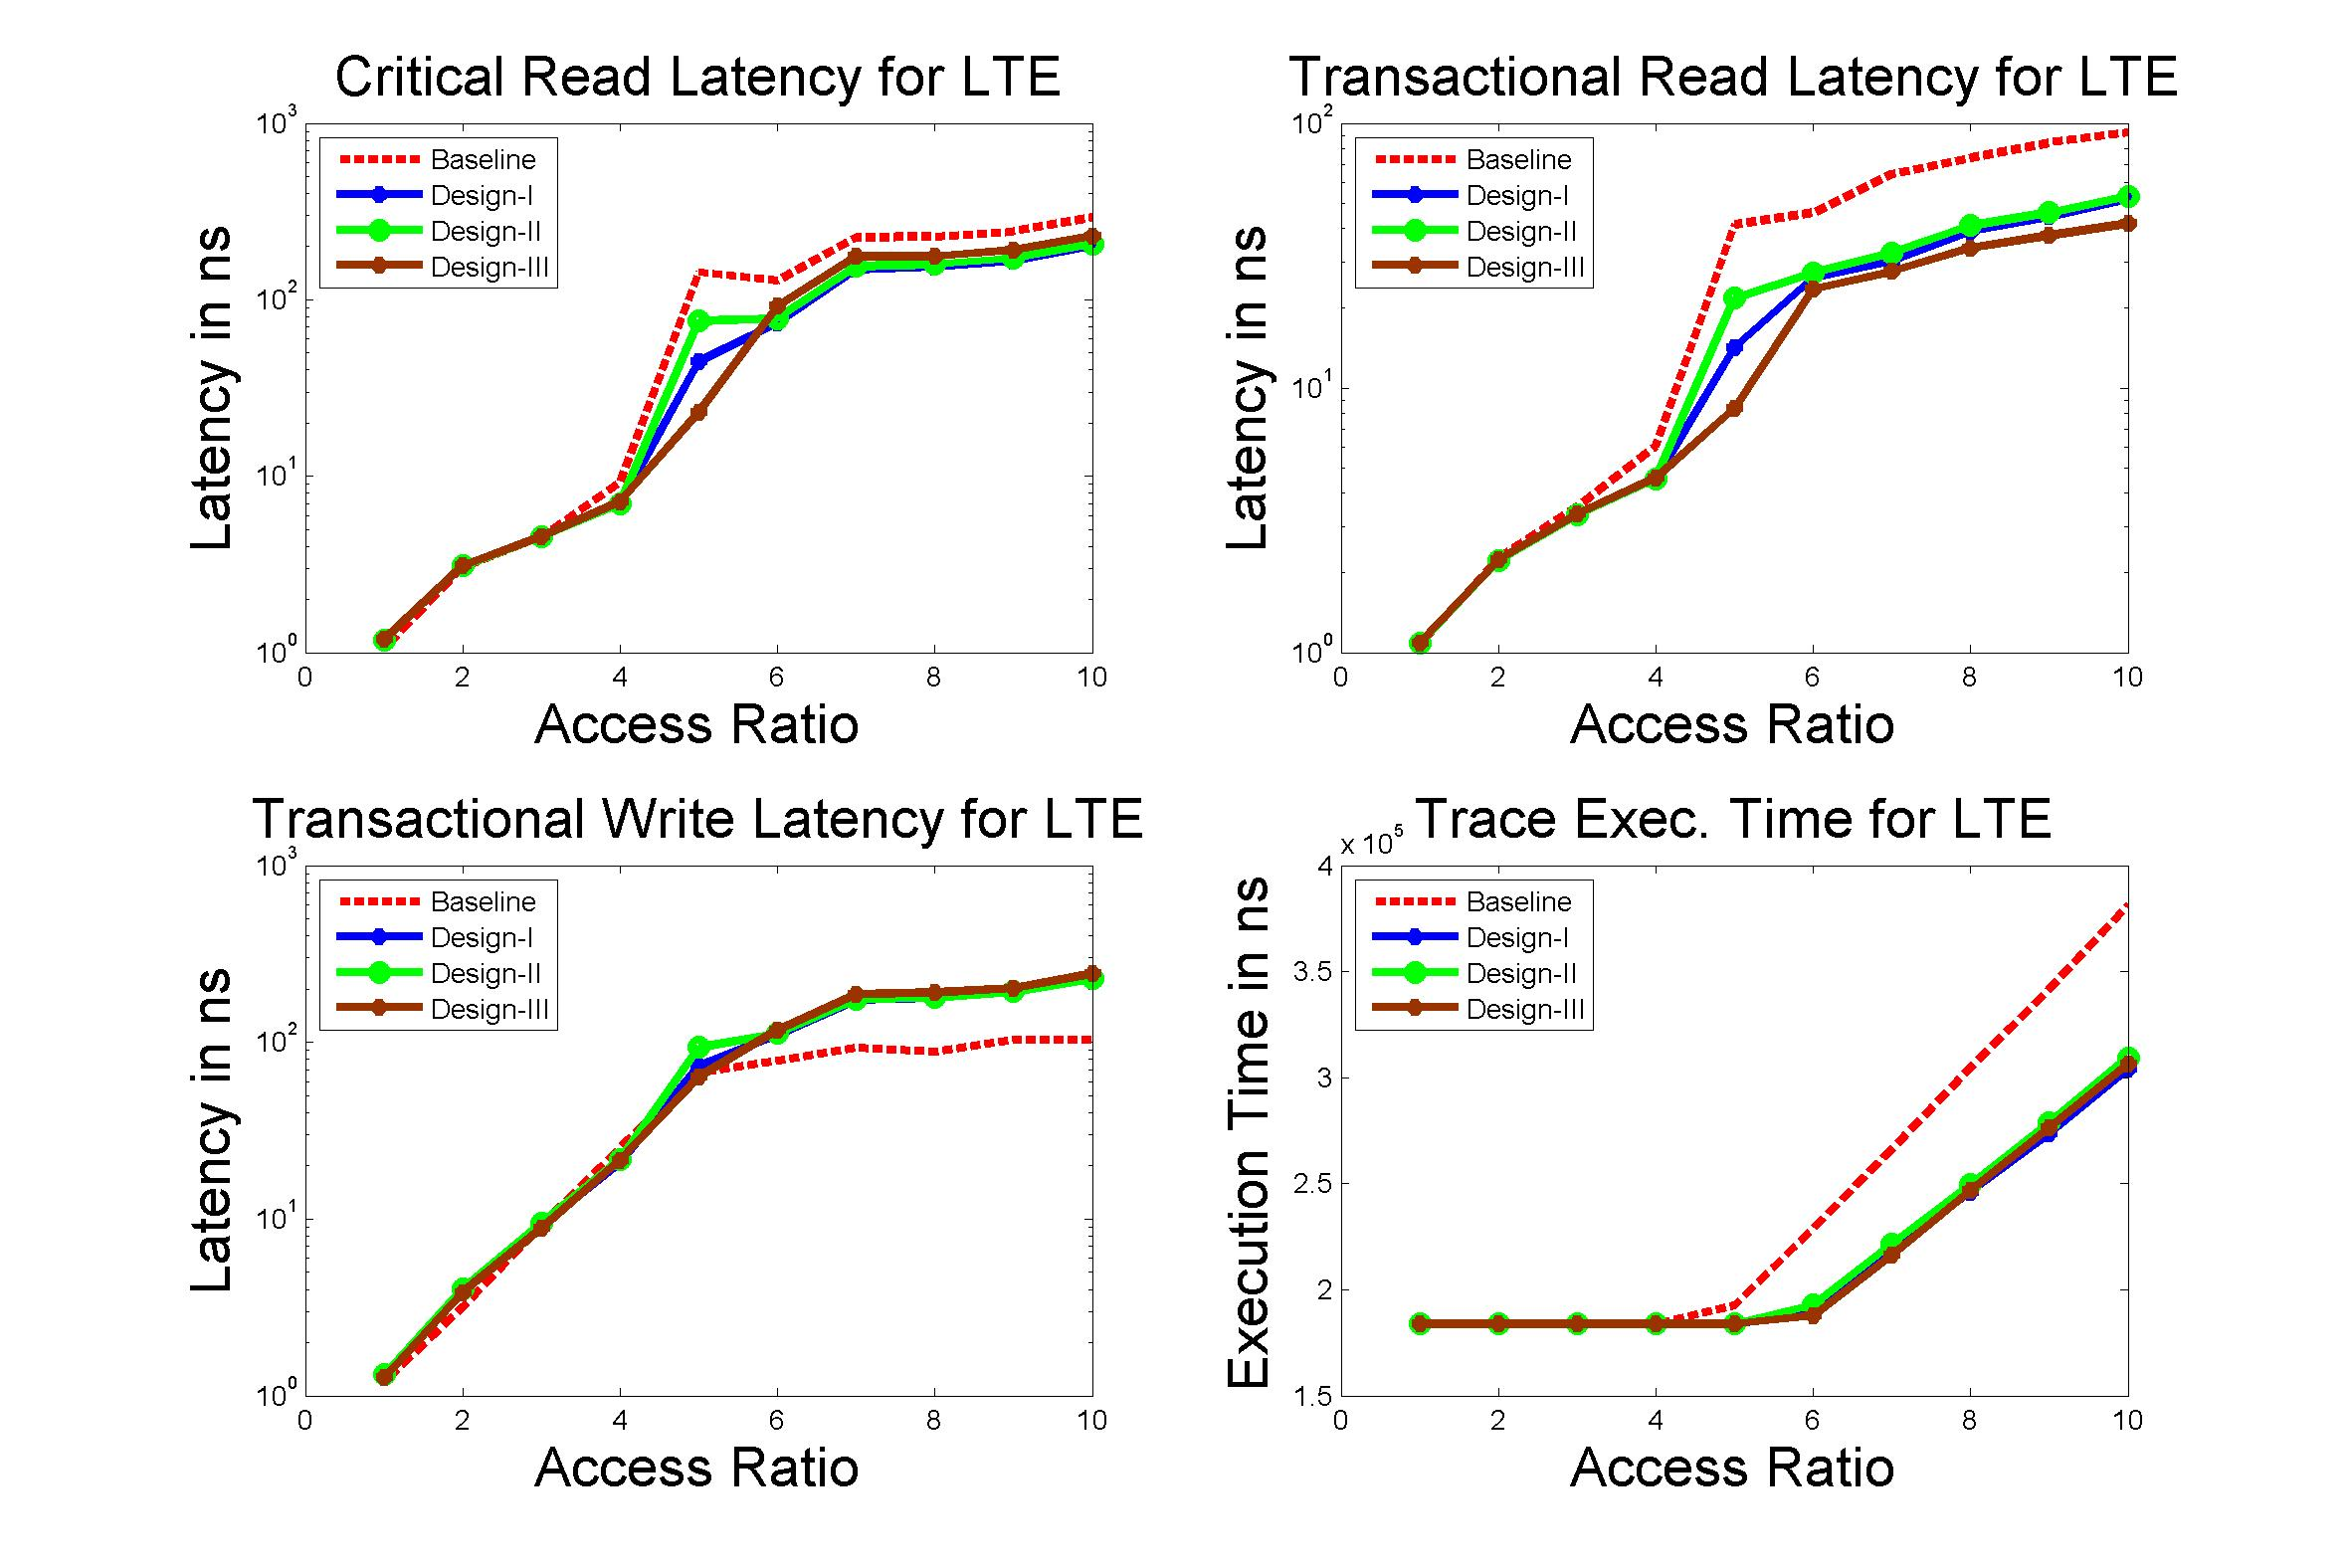
\includegraphics[width=\linewidth]{LTE.jpg}
\end{minipage}
\caption{
{\bf Performance Graphs for LTE trace} }
\label{fig:LTE}
\end{figure}
%-------------------------------------------------
\cleardoublepage
%-------------------------------------------------
\begin{figure}[htb]
%	\centering
\begin{minipage}[!t]{0.33\linewidth}
        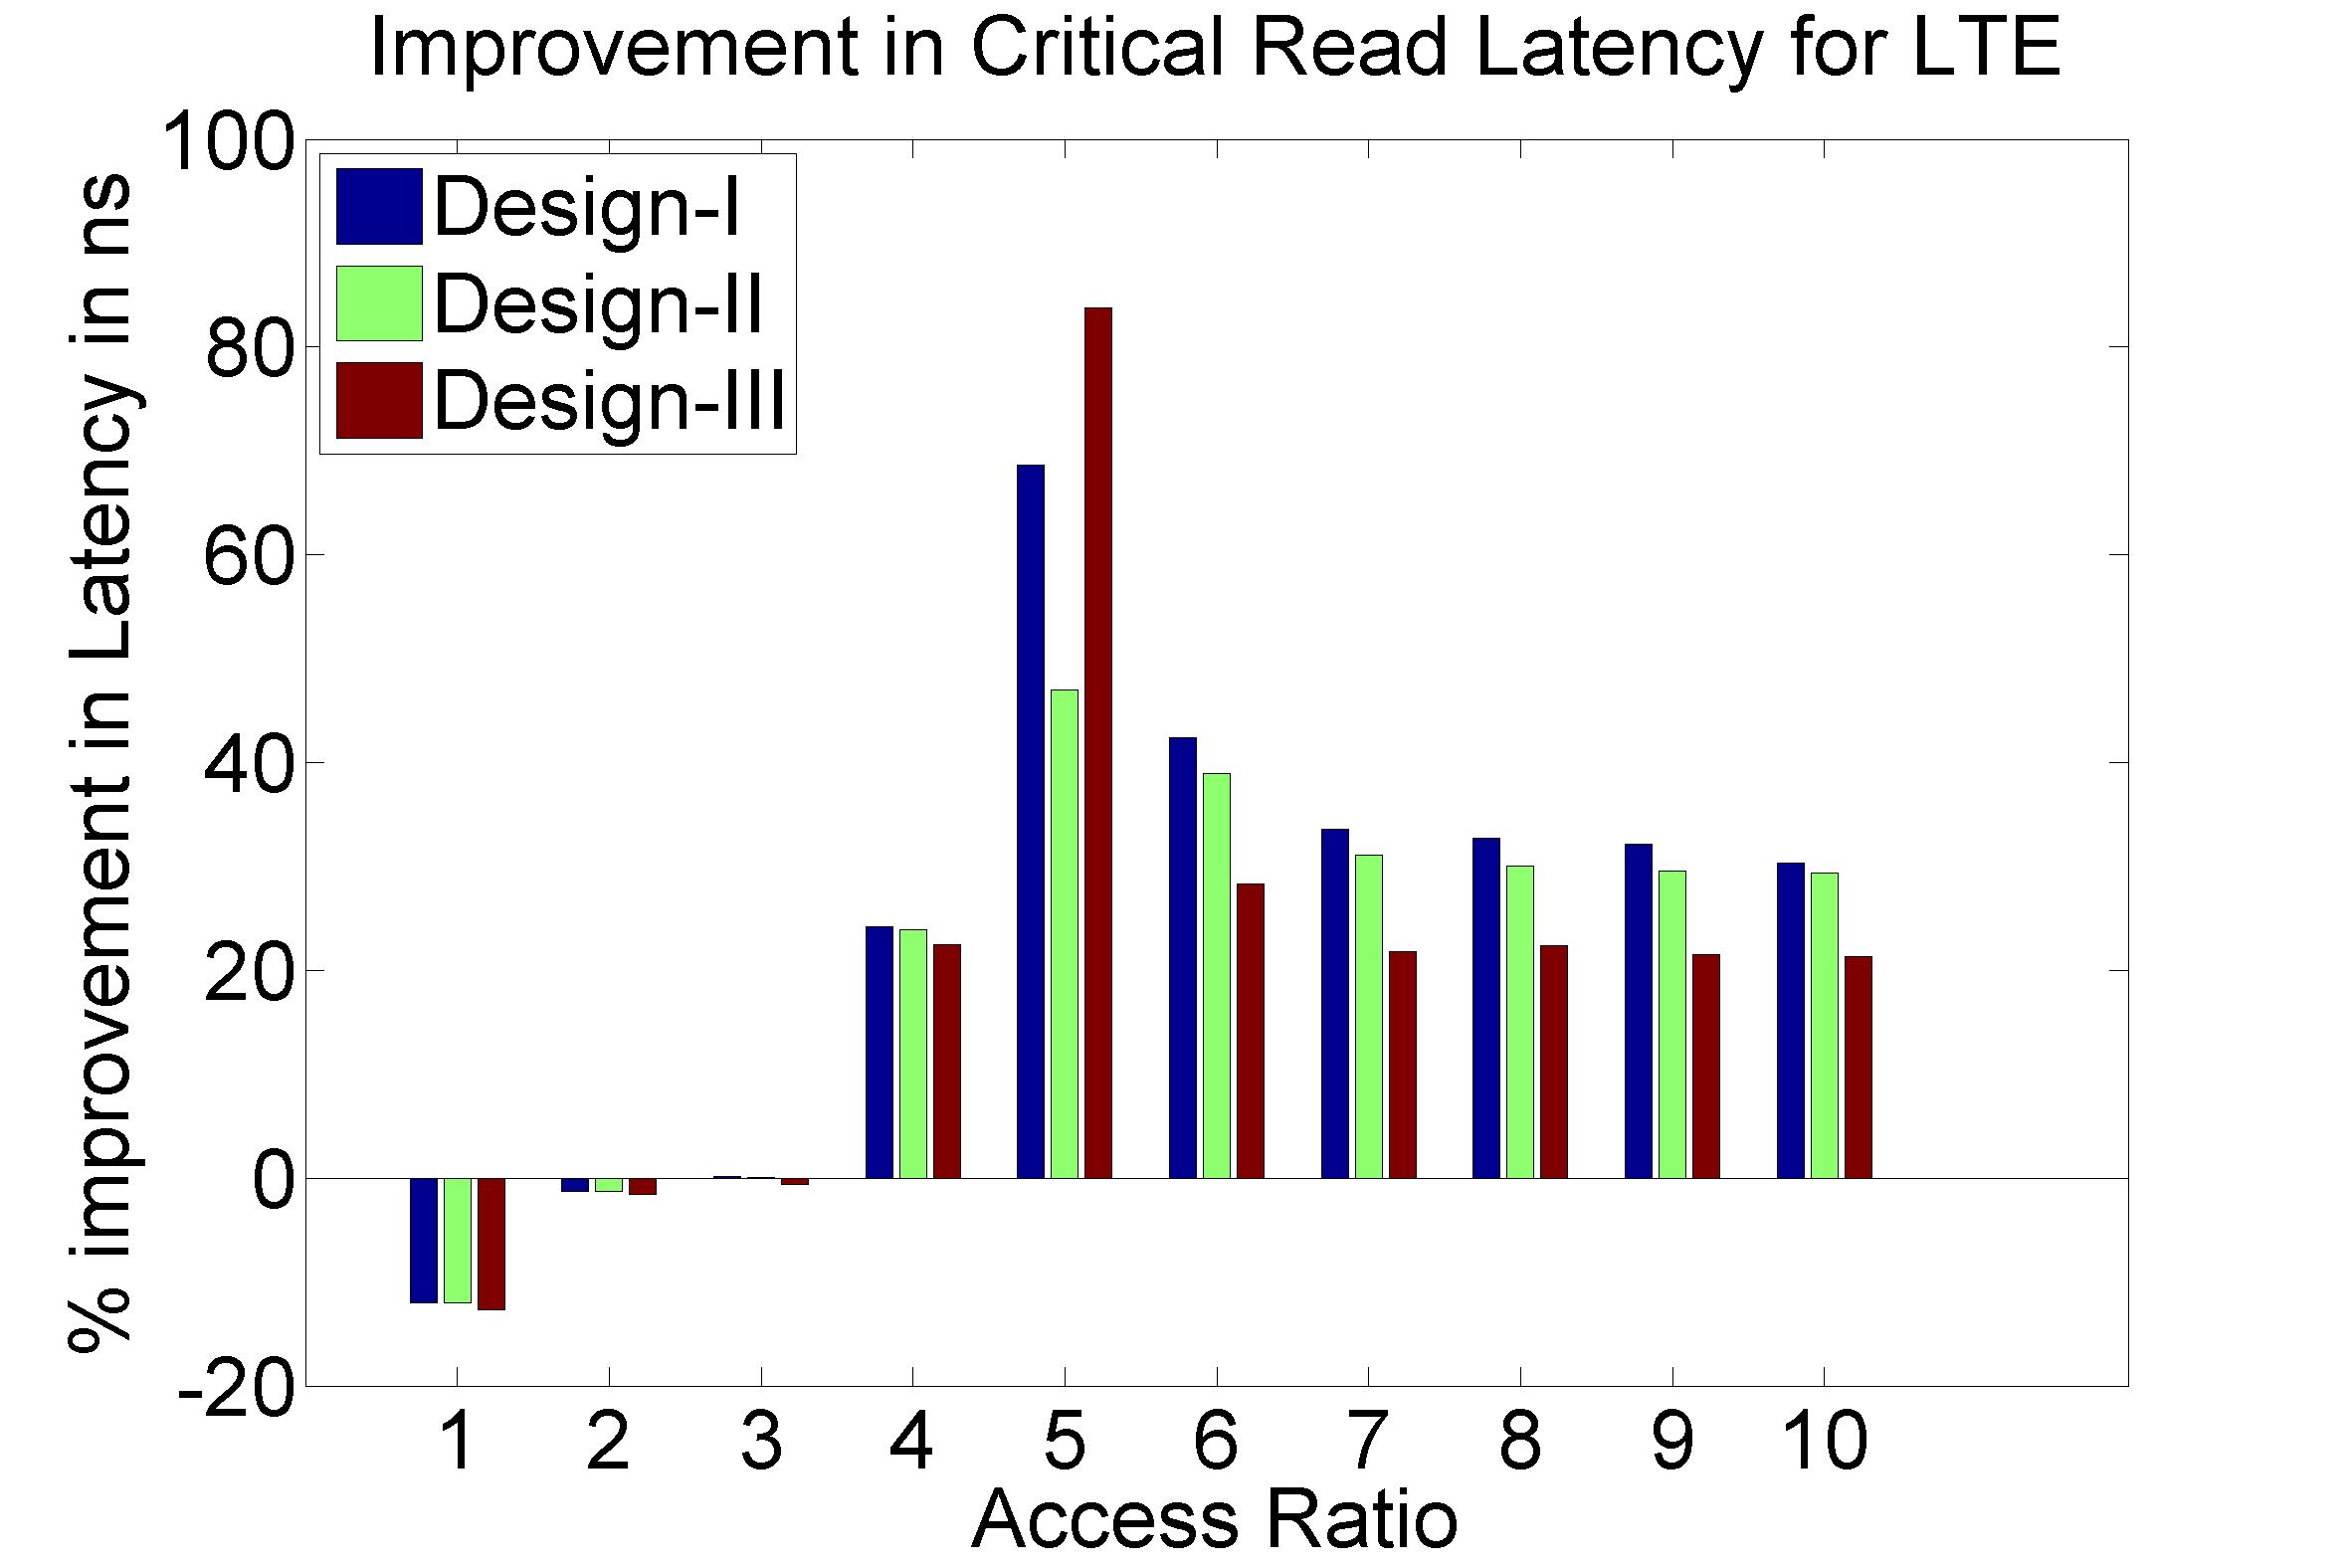
\includegraphics[width=\linewidth]{LTE_critical_latency_improvement.jpeg}
\end{minipage}
\begin{minipage}[!t]{0.33\linewidth}
        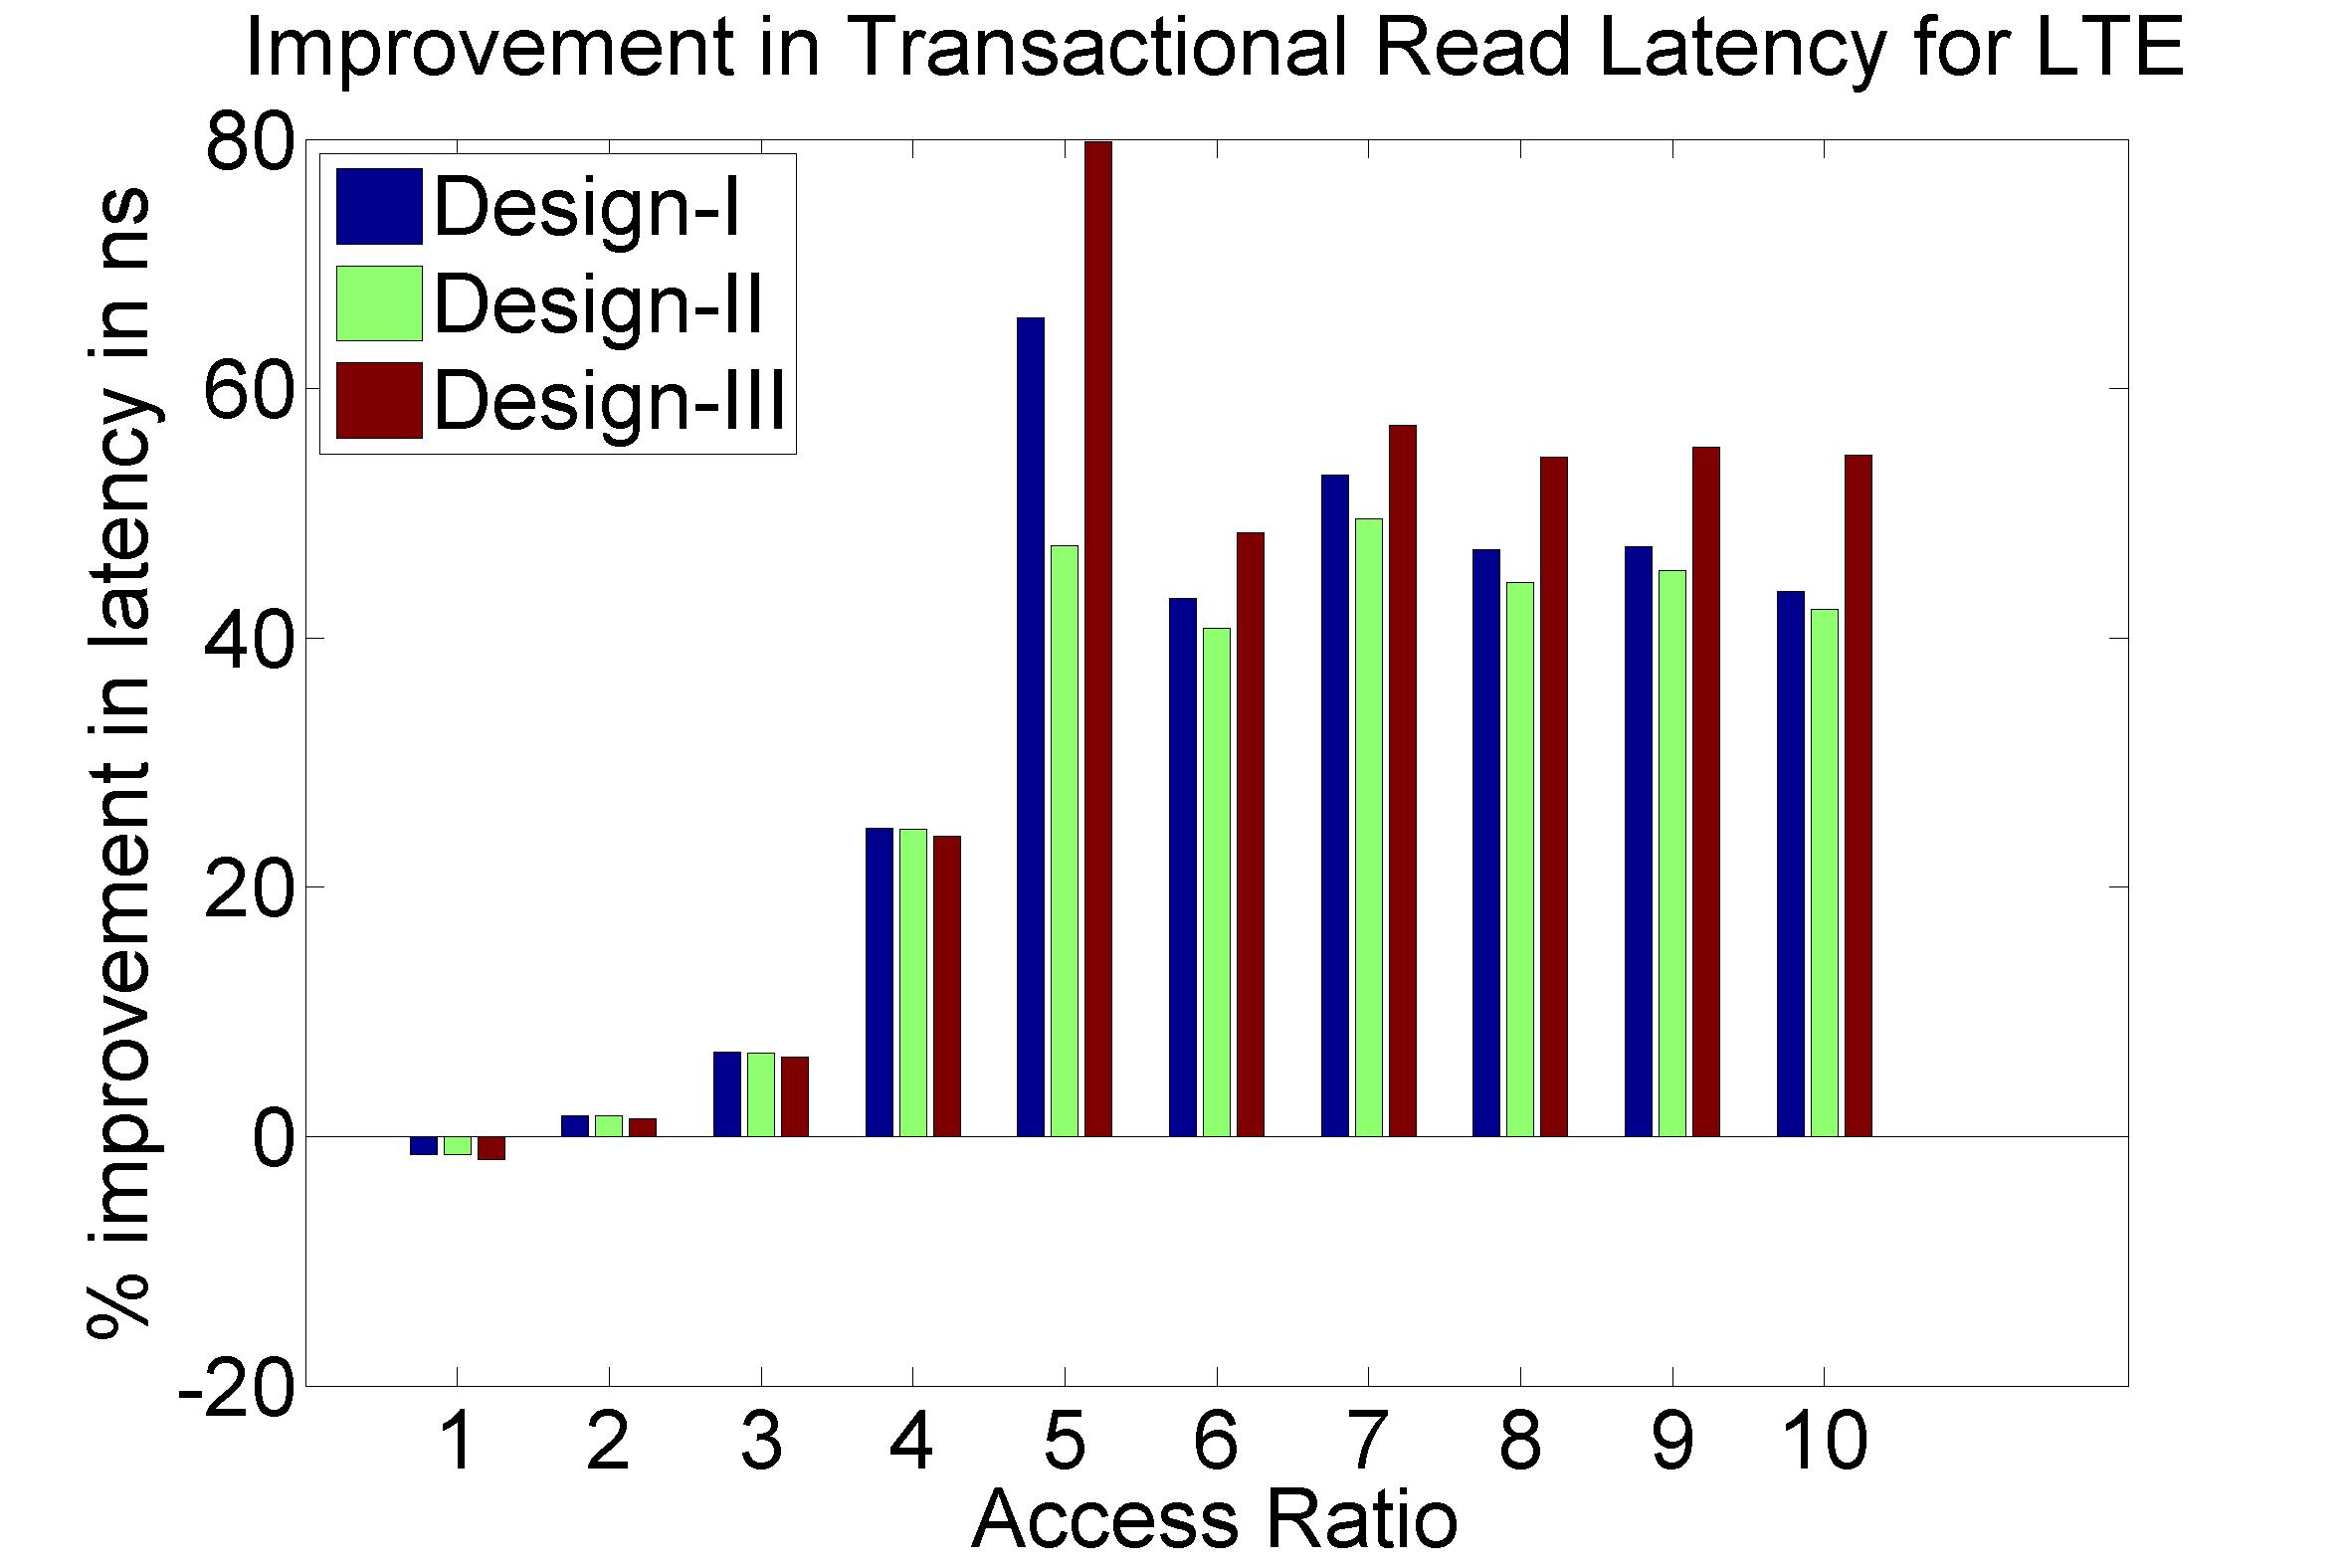
\includegraphics[width=\linewidth]{LTE_transactional_latency_improvement.jpeg}
\end{minipage}
\begin{minipage}[!t]{0.33\linewidth}
        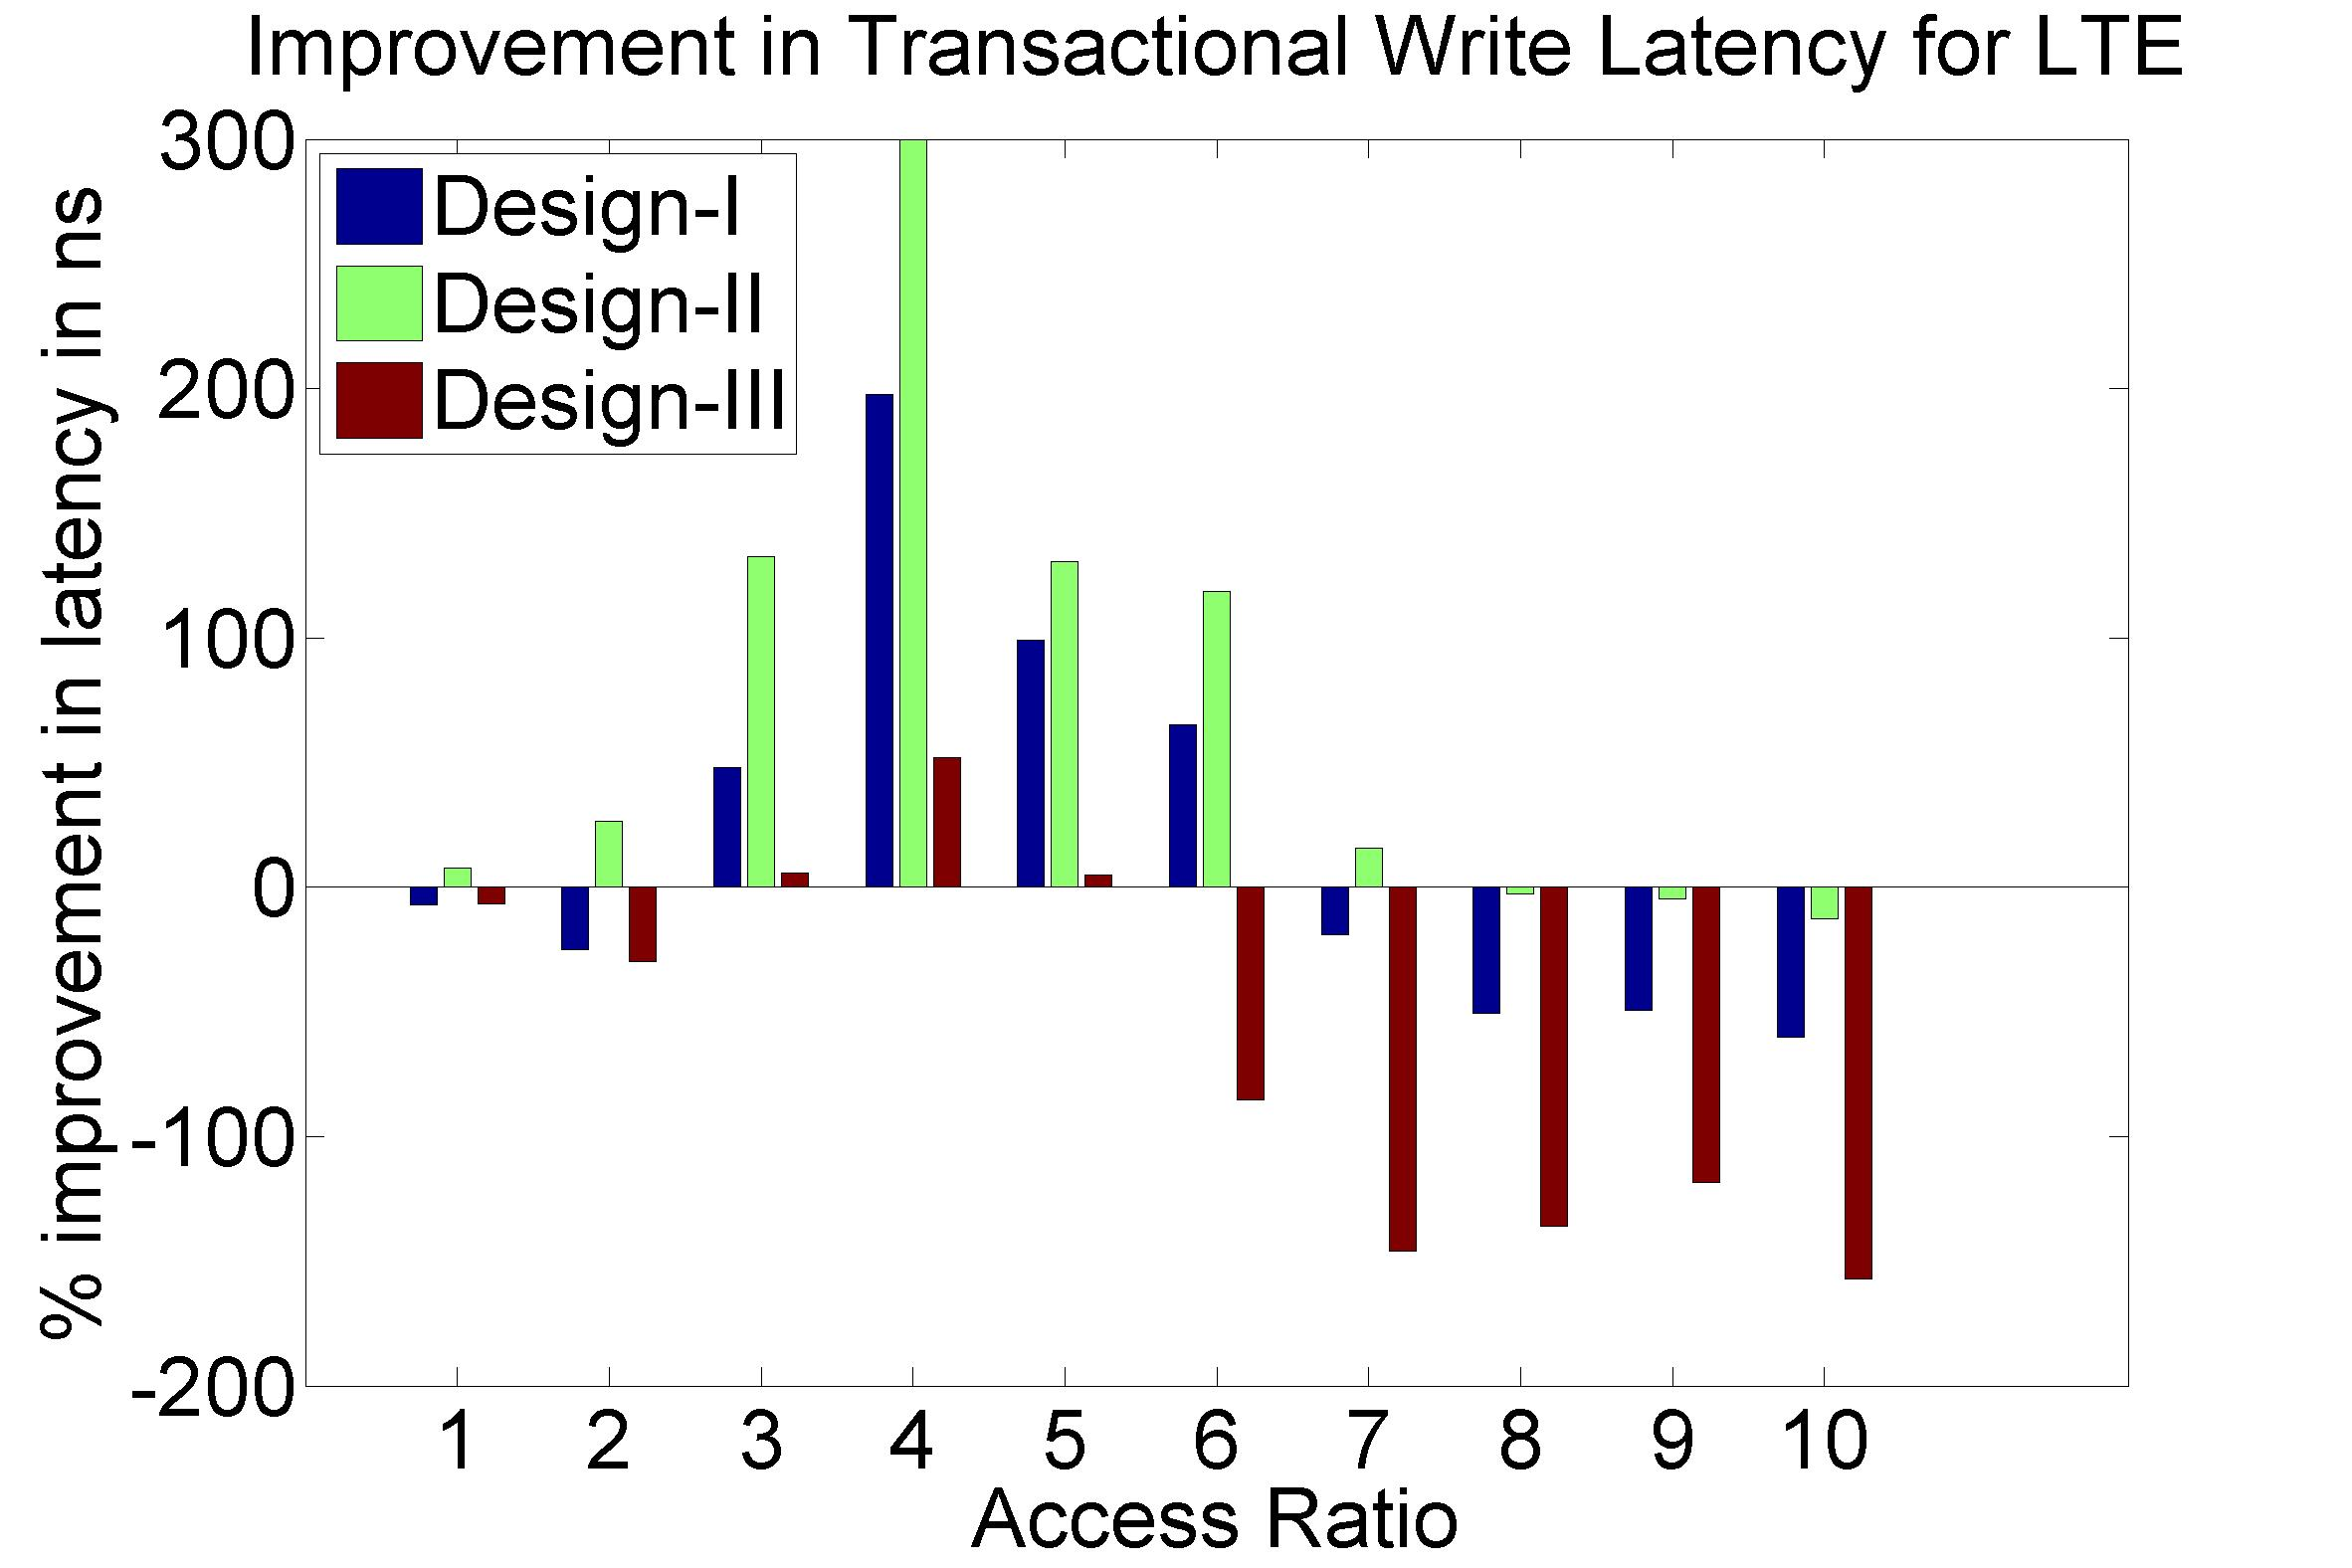
\includegraphics[width=\linewidth]{LTE_write_latency_improvement.jpeg}
\end{minipage}
\caption{
{\bf Performance Graphs for LTE trace} }
\label{fig:LTE_improvement}
\end{figure}
%-------------------------------------------------
Observations:
\begin{itemize}
	\item LTE trace is a medium density trace.
	\item The benefit for coding for read access is favourable for access ratios for 4 and more. 
	\item The write transaction latency shows improvement for access ratios of 3 to 6.
	\item The coding benefits are best at access ratio of 4, 5 and 6.
\end{itemize}
\cleardoublepage
%-------------------------------------------------
\begin{figure}[htb]
\begin{minipage}[!t]{\linewidth}
        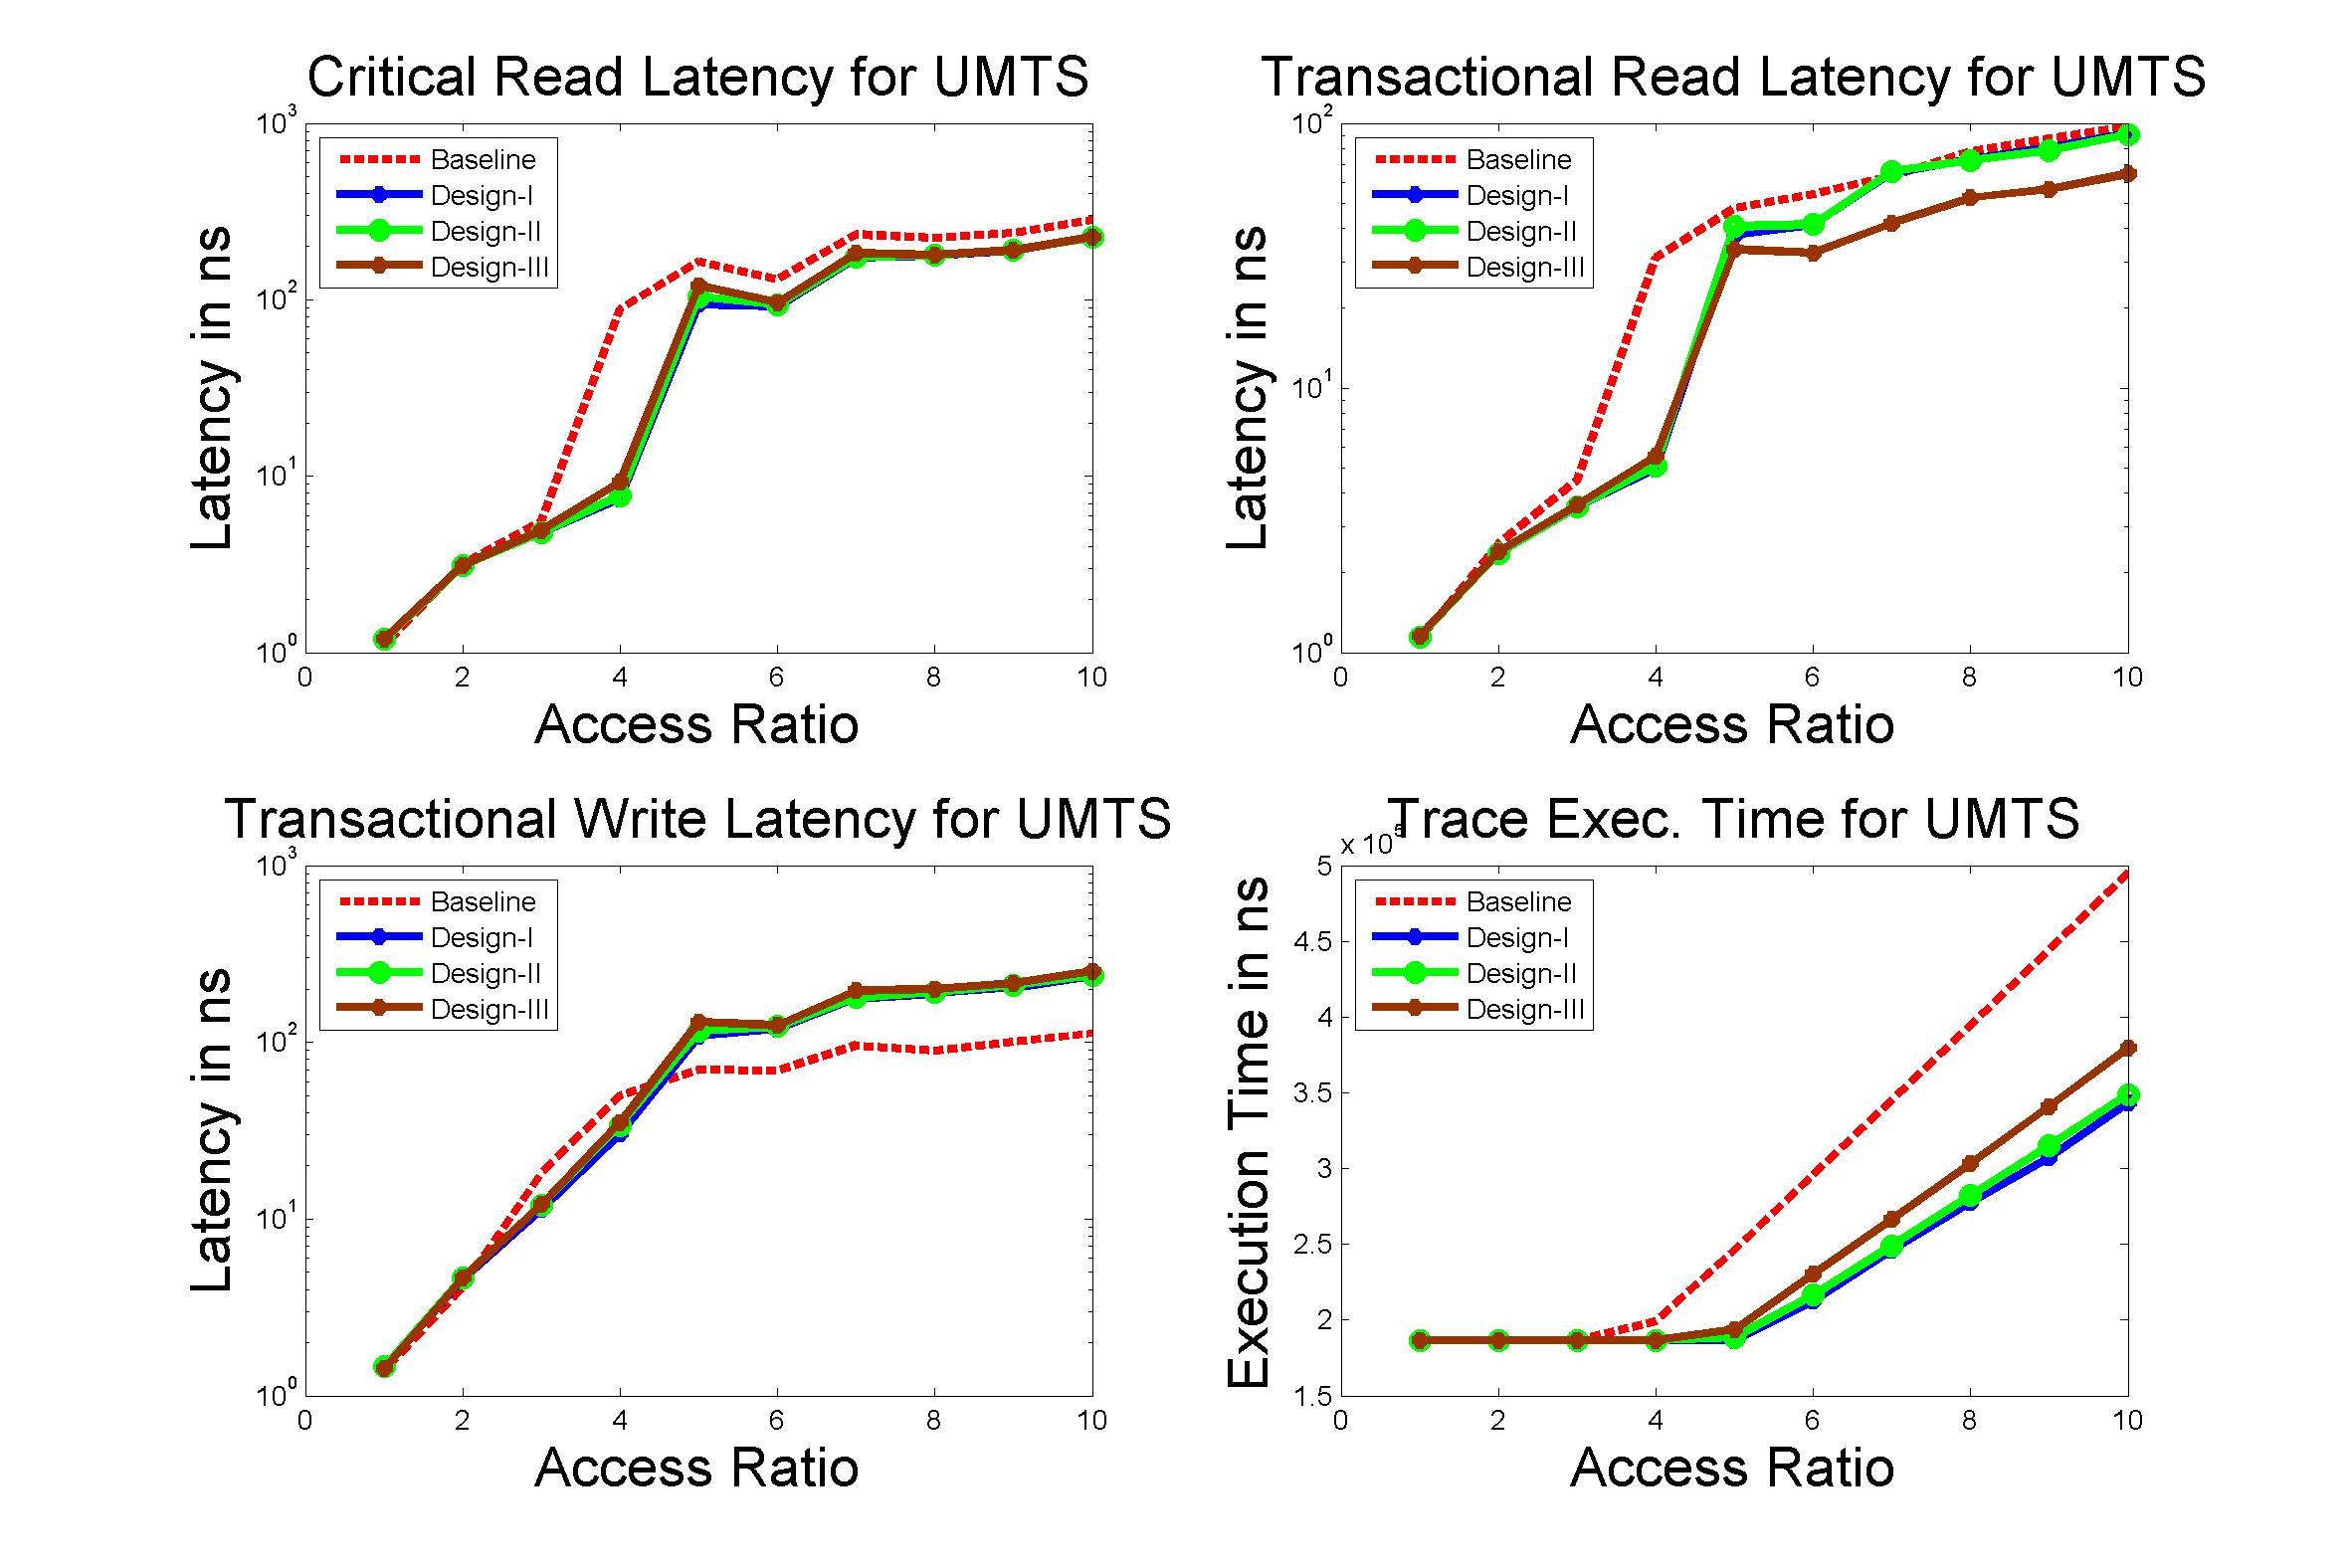
\includegraphics[width=\linewidth]{UMTS.jpg}
\end{minipage}
\caption{
{\bf Performance Graphs for UMTS trace} }
\label{fig:LTE}
\end{figure}
%-------------------------------------------------
\cleardoublepage
%-------------------------------------------------
\begin{figure}[htb]
\begin{minipage}[!t]{0.33\linewidth}
        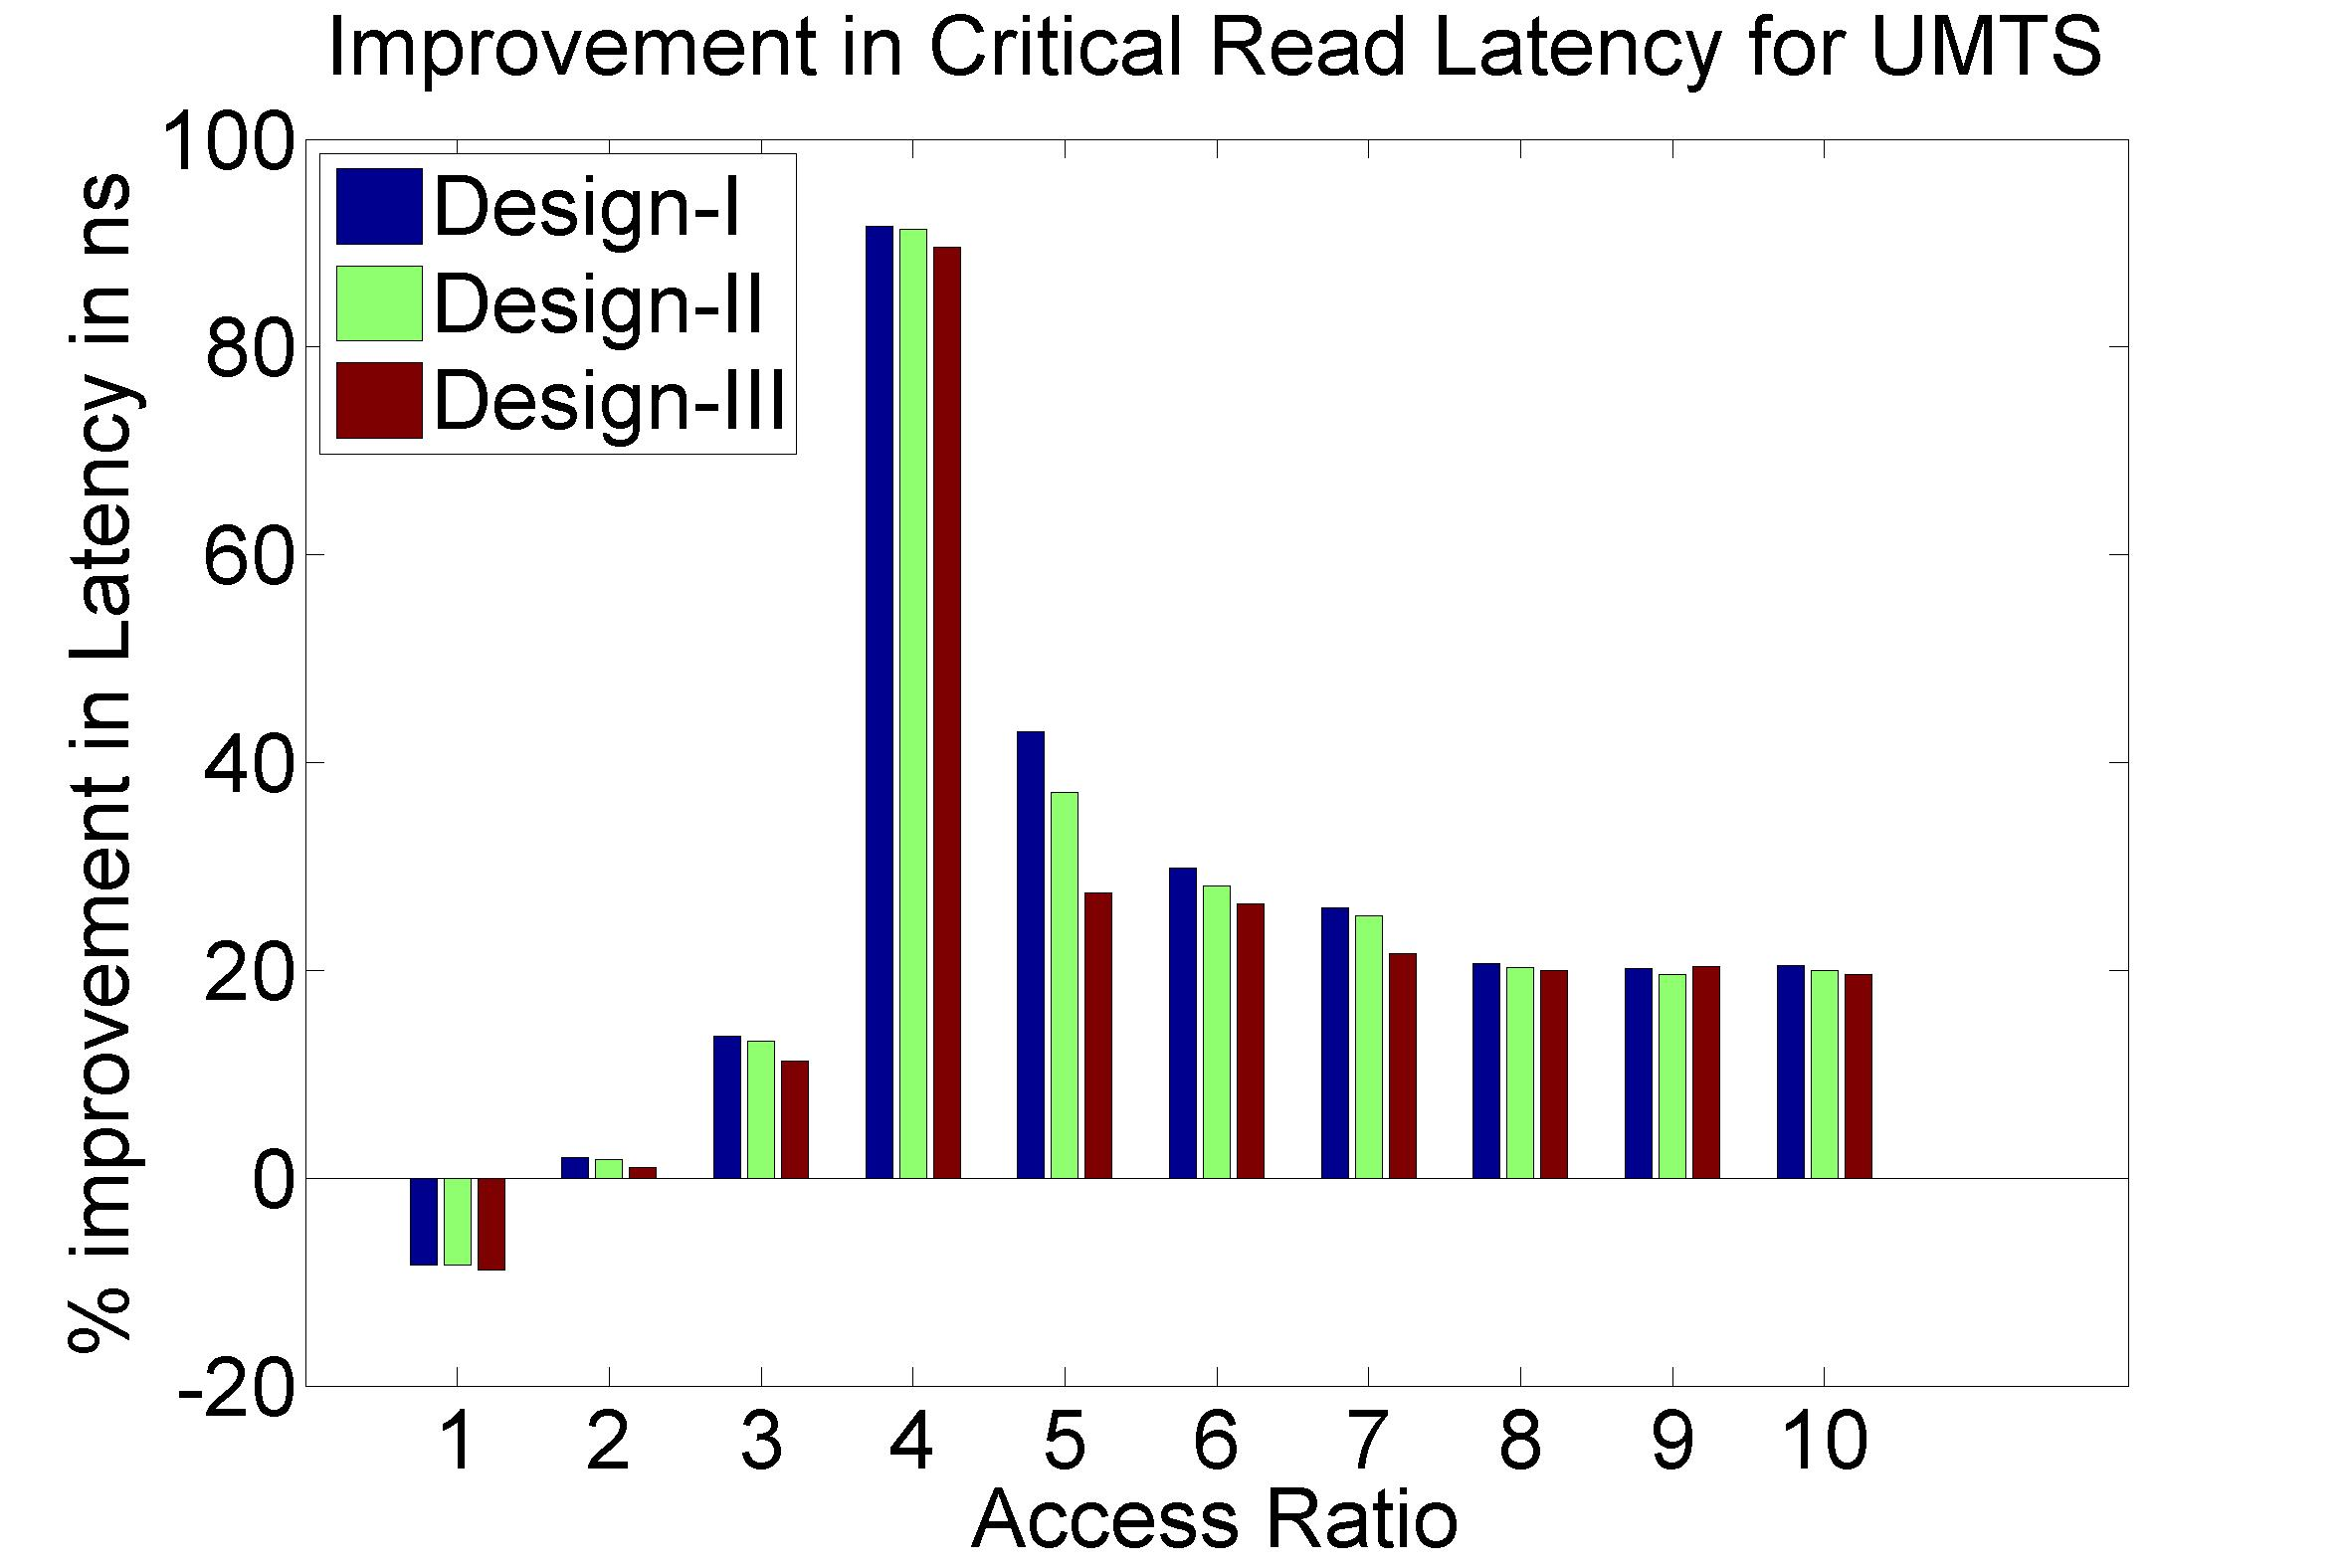
\includegraphics[width=\linewidth]{UMTS_critical_latency_improvement.jpeg}
\end{minipage}
\begin{minipage}[!t]{0.33\linewidth}
        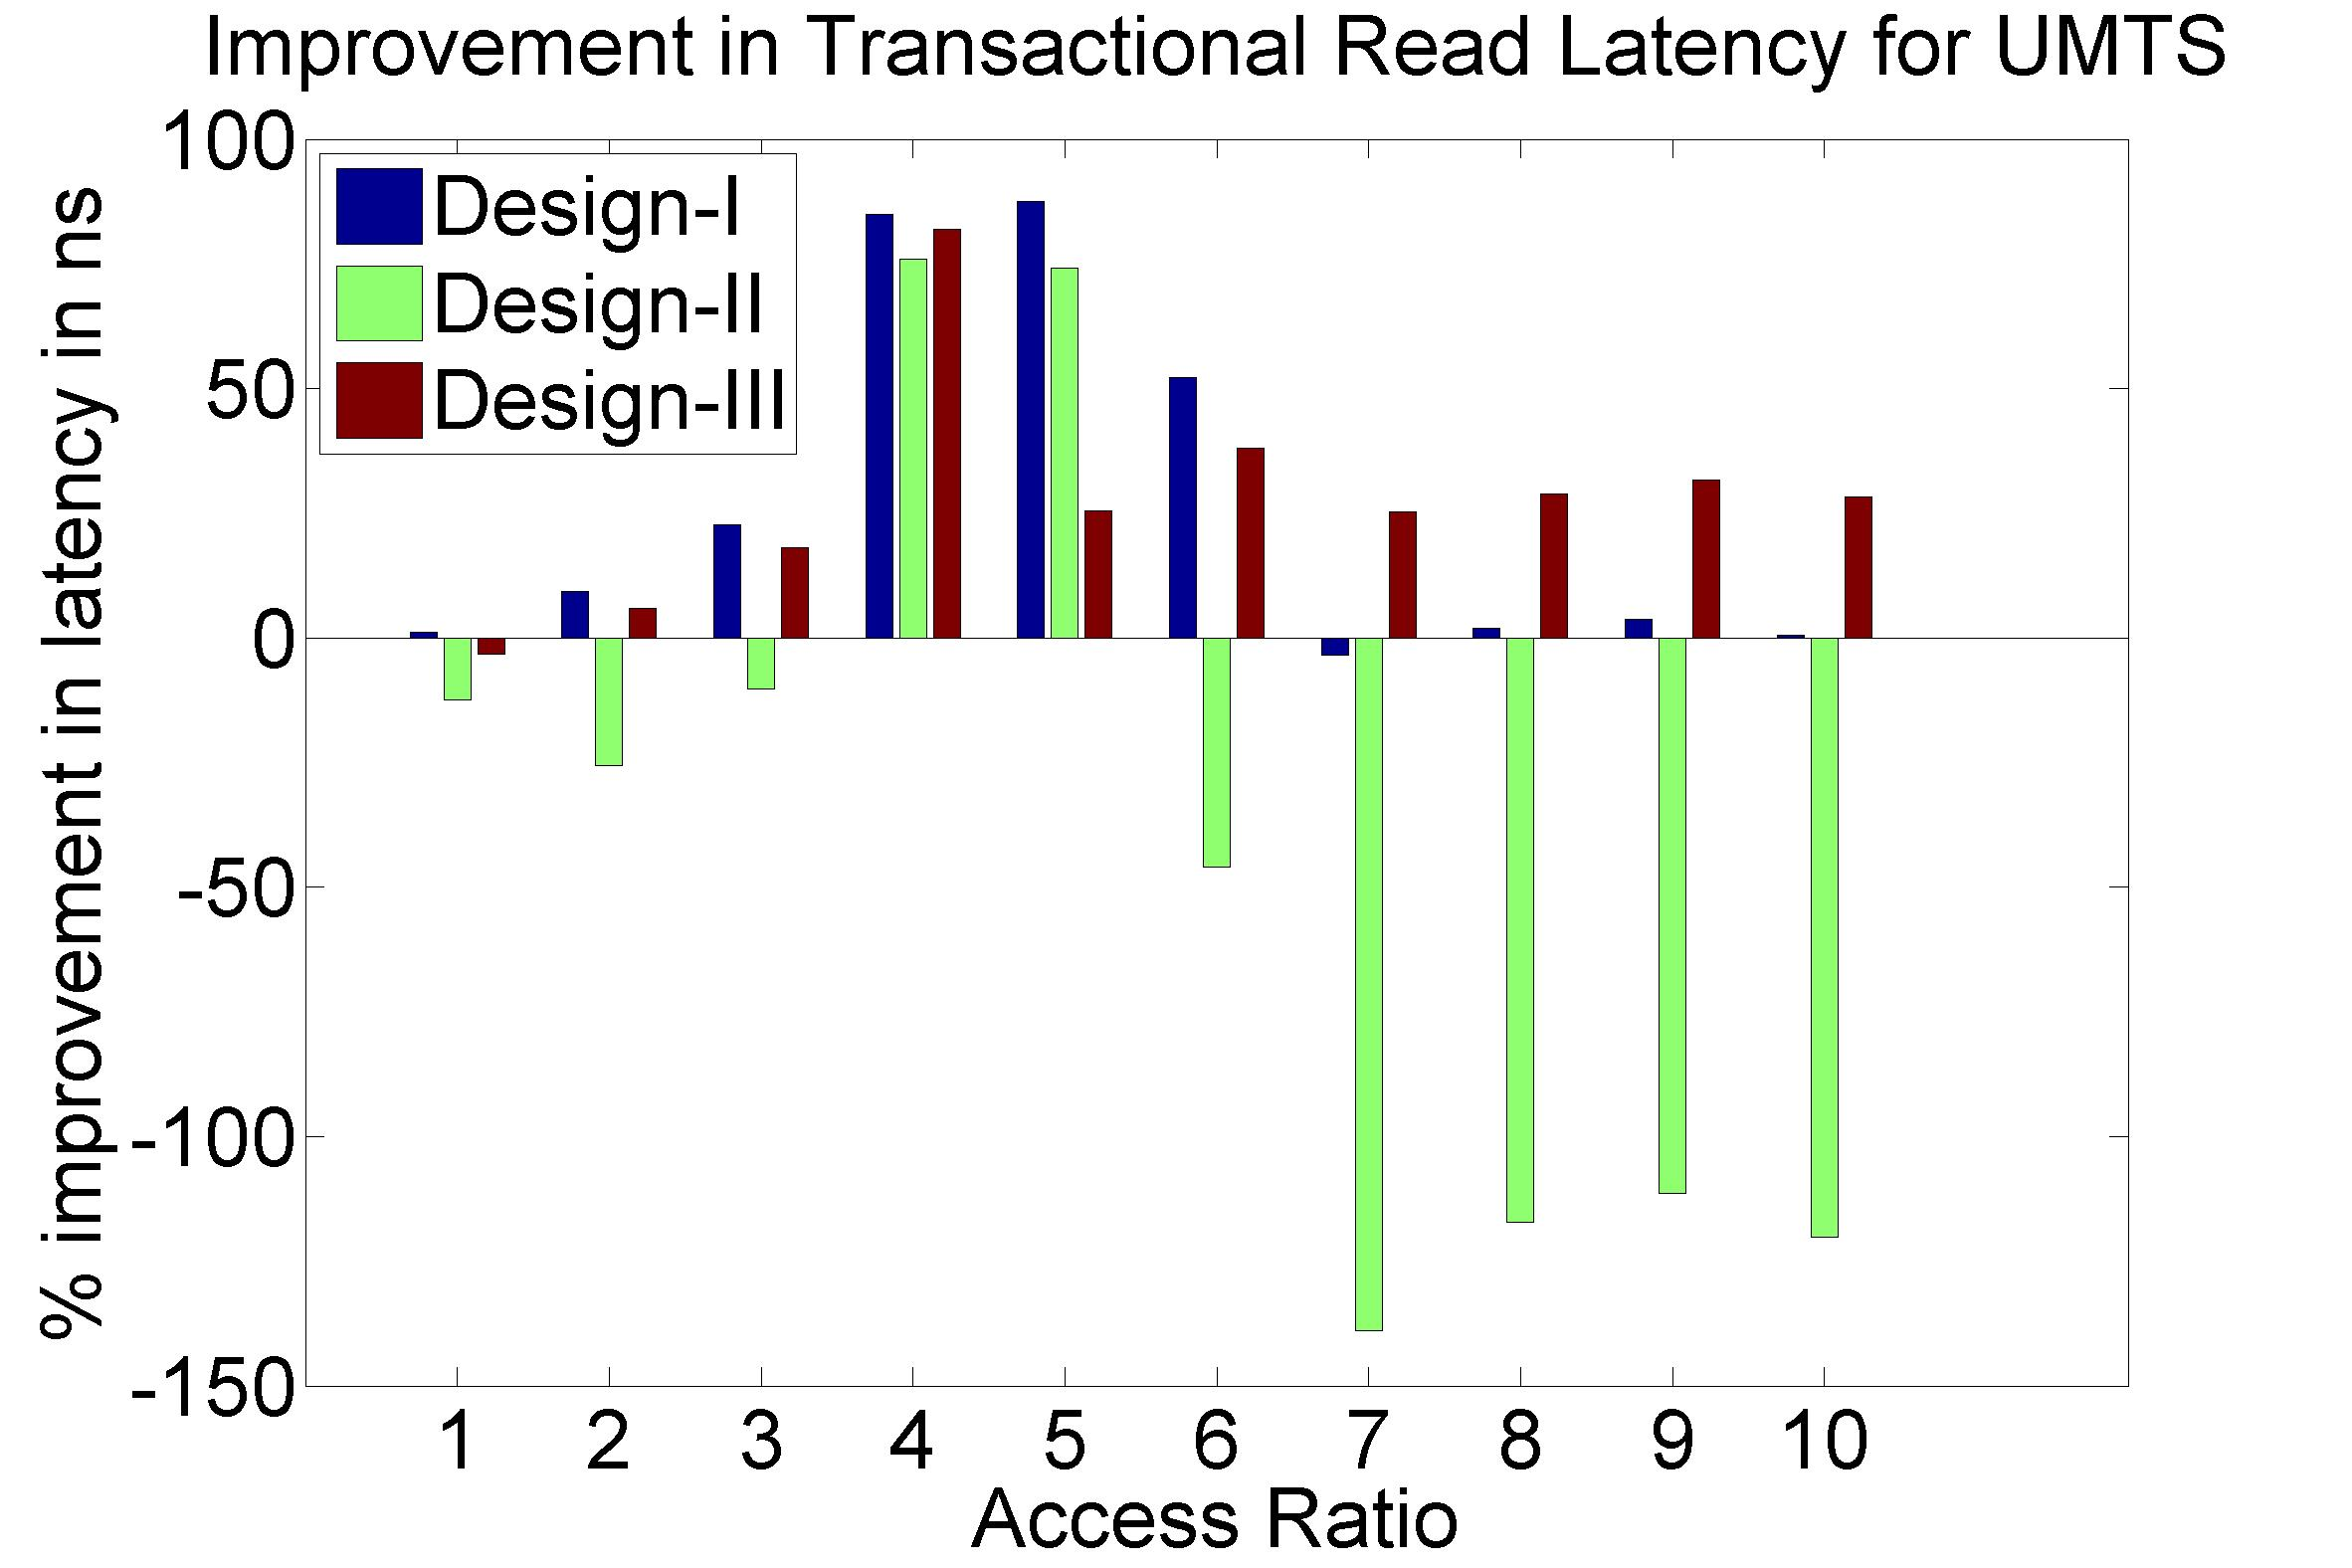
\includegraphics[width=\linewidth]{UMTS_transactional_latency_improvement.jpeg}
\end{minipage}
\begin{minipage}[!t]{0.33\linewidth}
        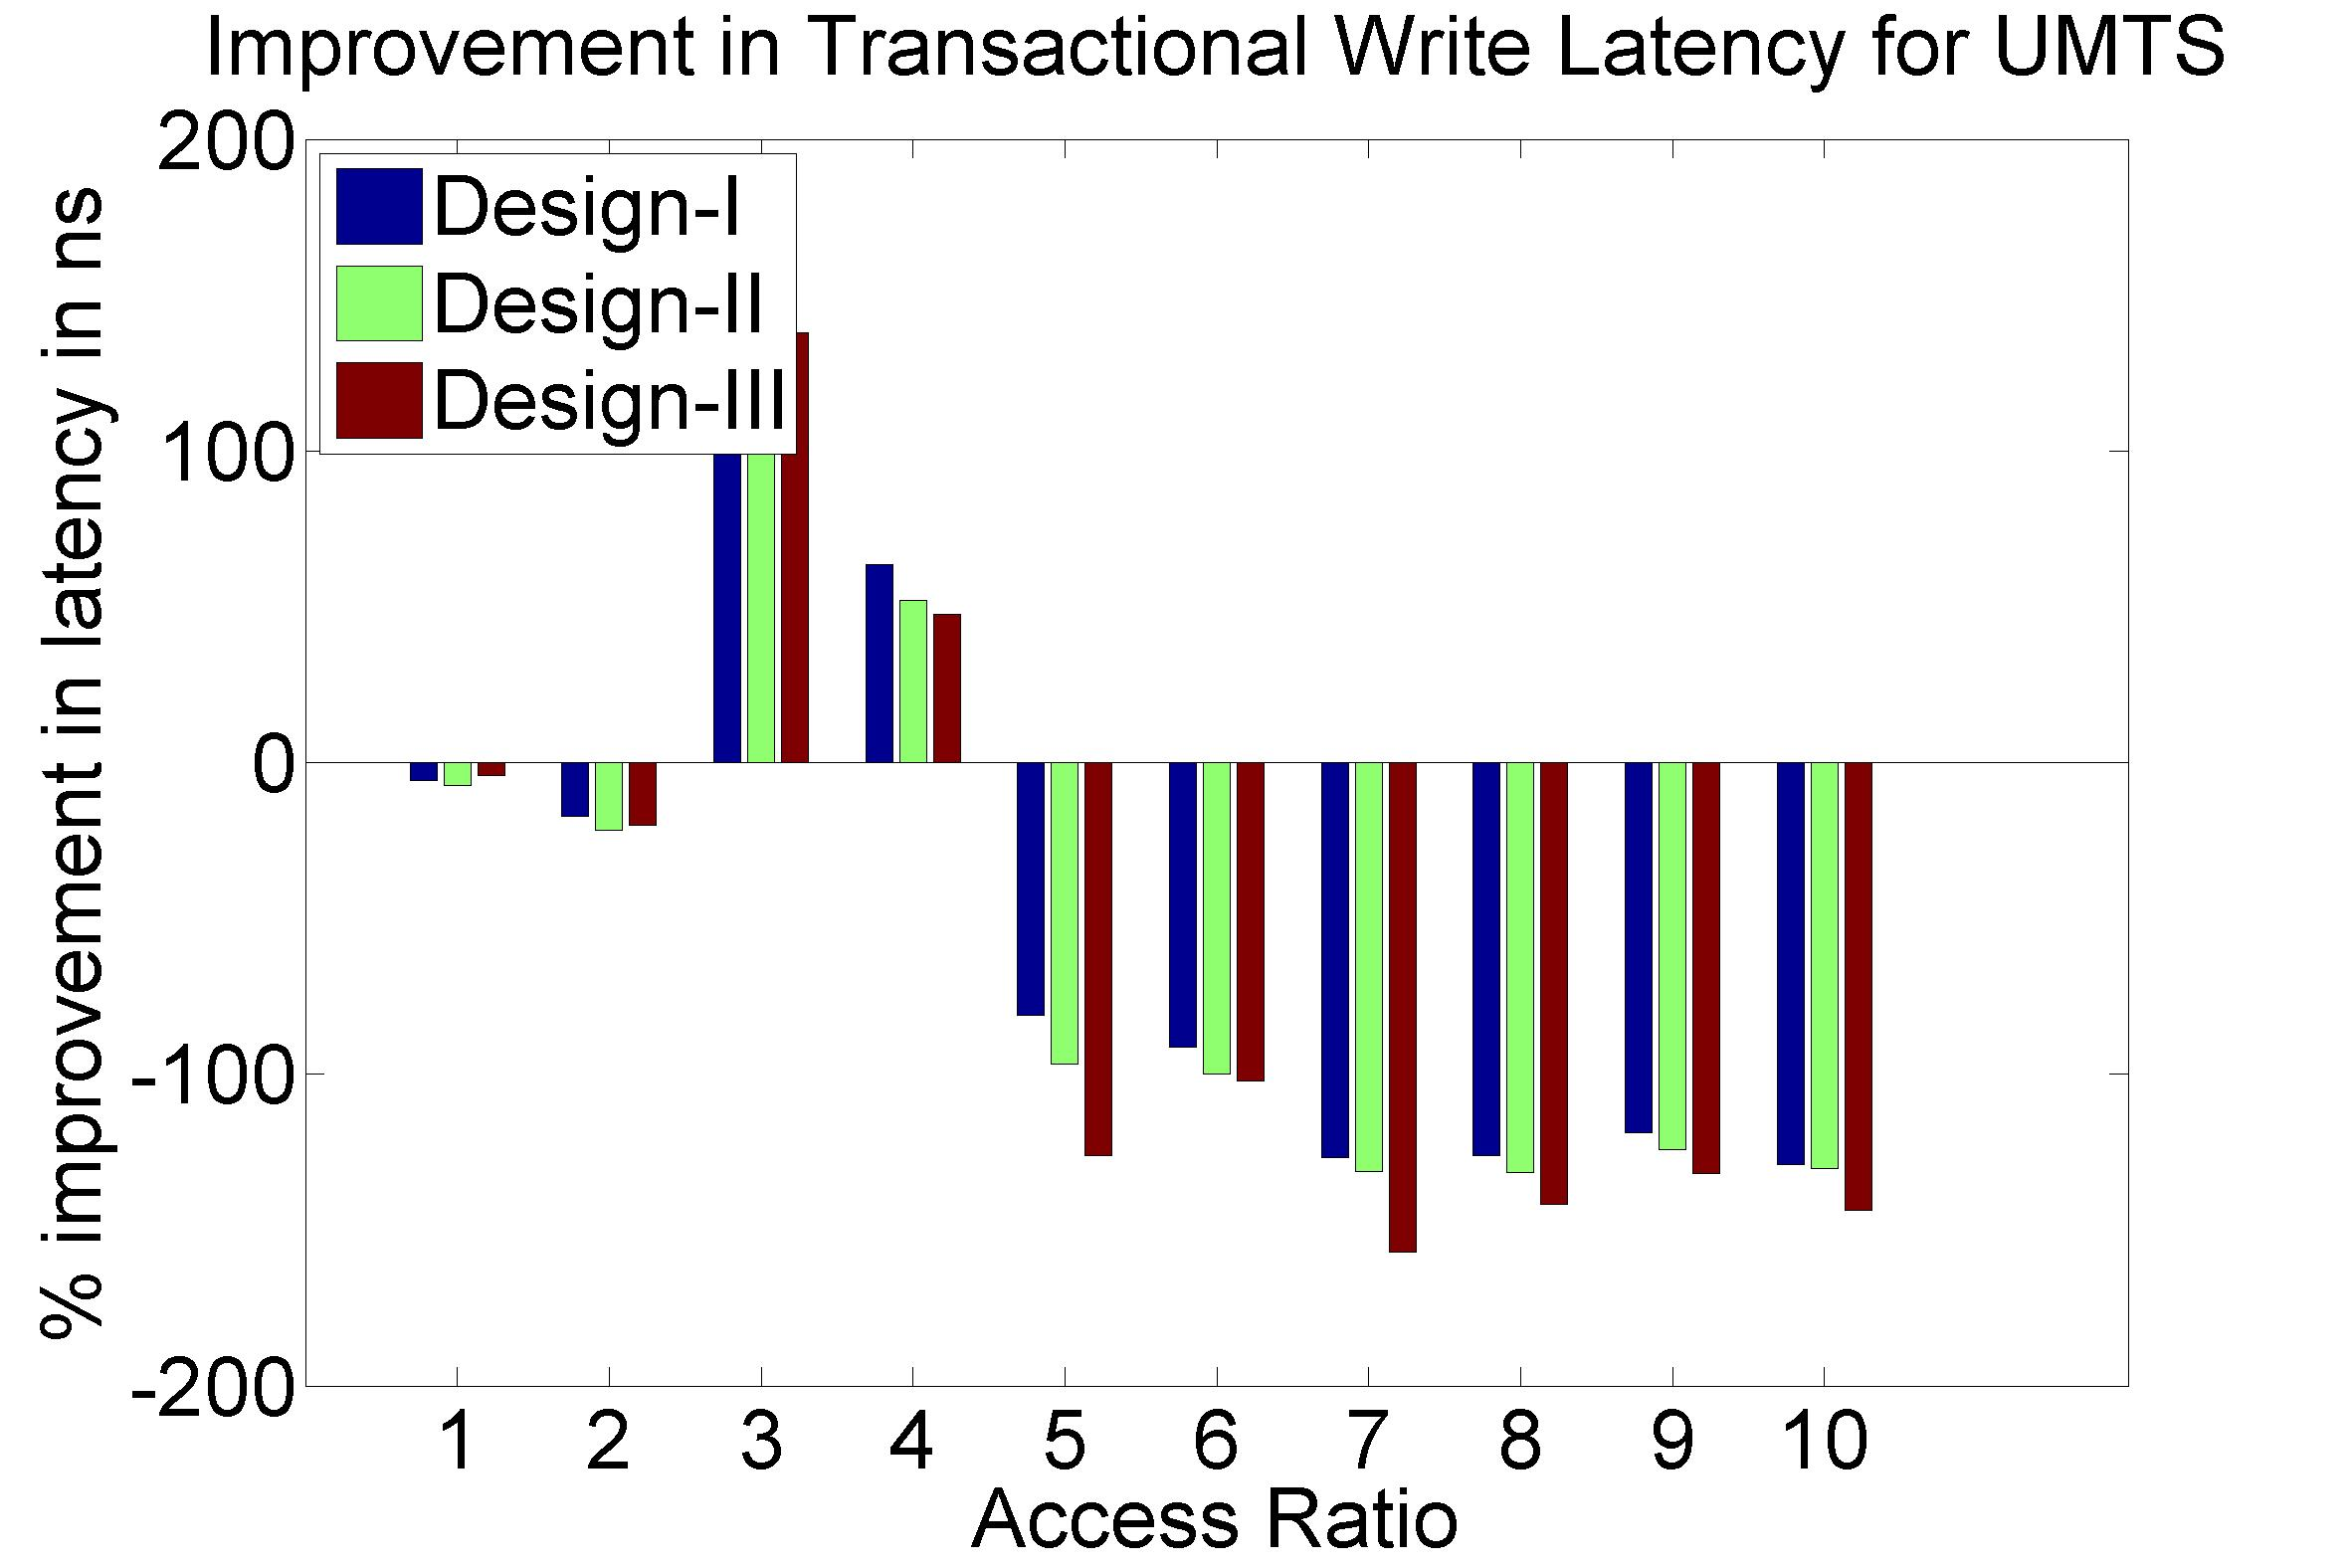
\includegraphics[width=\linewidth]{UMTS_write_latency_improvement.jpeg}
\end{minipage}
\caption{
{\bf Performance Graphs for UMTS trace} }
\label{fig:UMTS_improvement}
\end{figure}
%-------------------------------------------------
Observations:
\begin{itemize}
	\item The UMTS trace is also a medium access trace. 
	\item The read latency improvement in UMTS is substantial for all access ratios in case of critical latency. 
	\item The Transactional Latency improvees untill access ratio of 6.
	\item The design II sees degradation in performance for higher access ratios. 
	\item Write Latency improvement is observed for access ratio of 3 and 4.
	\item The coding benefits are best at access ratio of 4.
\end{itemize}
\cleardoublepage
%-------------------------------------------------
\begin{figure}[htb]
\begin{minipage}[!t]{\linewidth}
        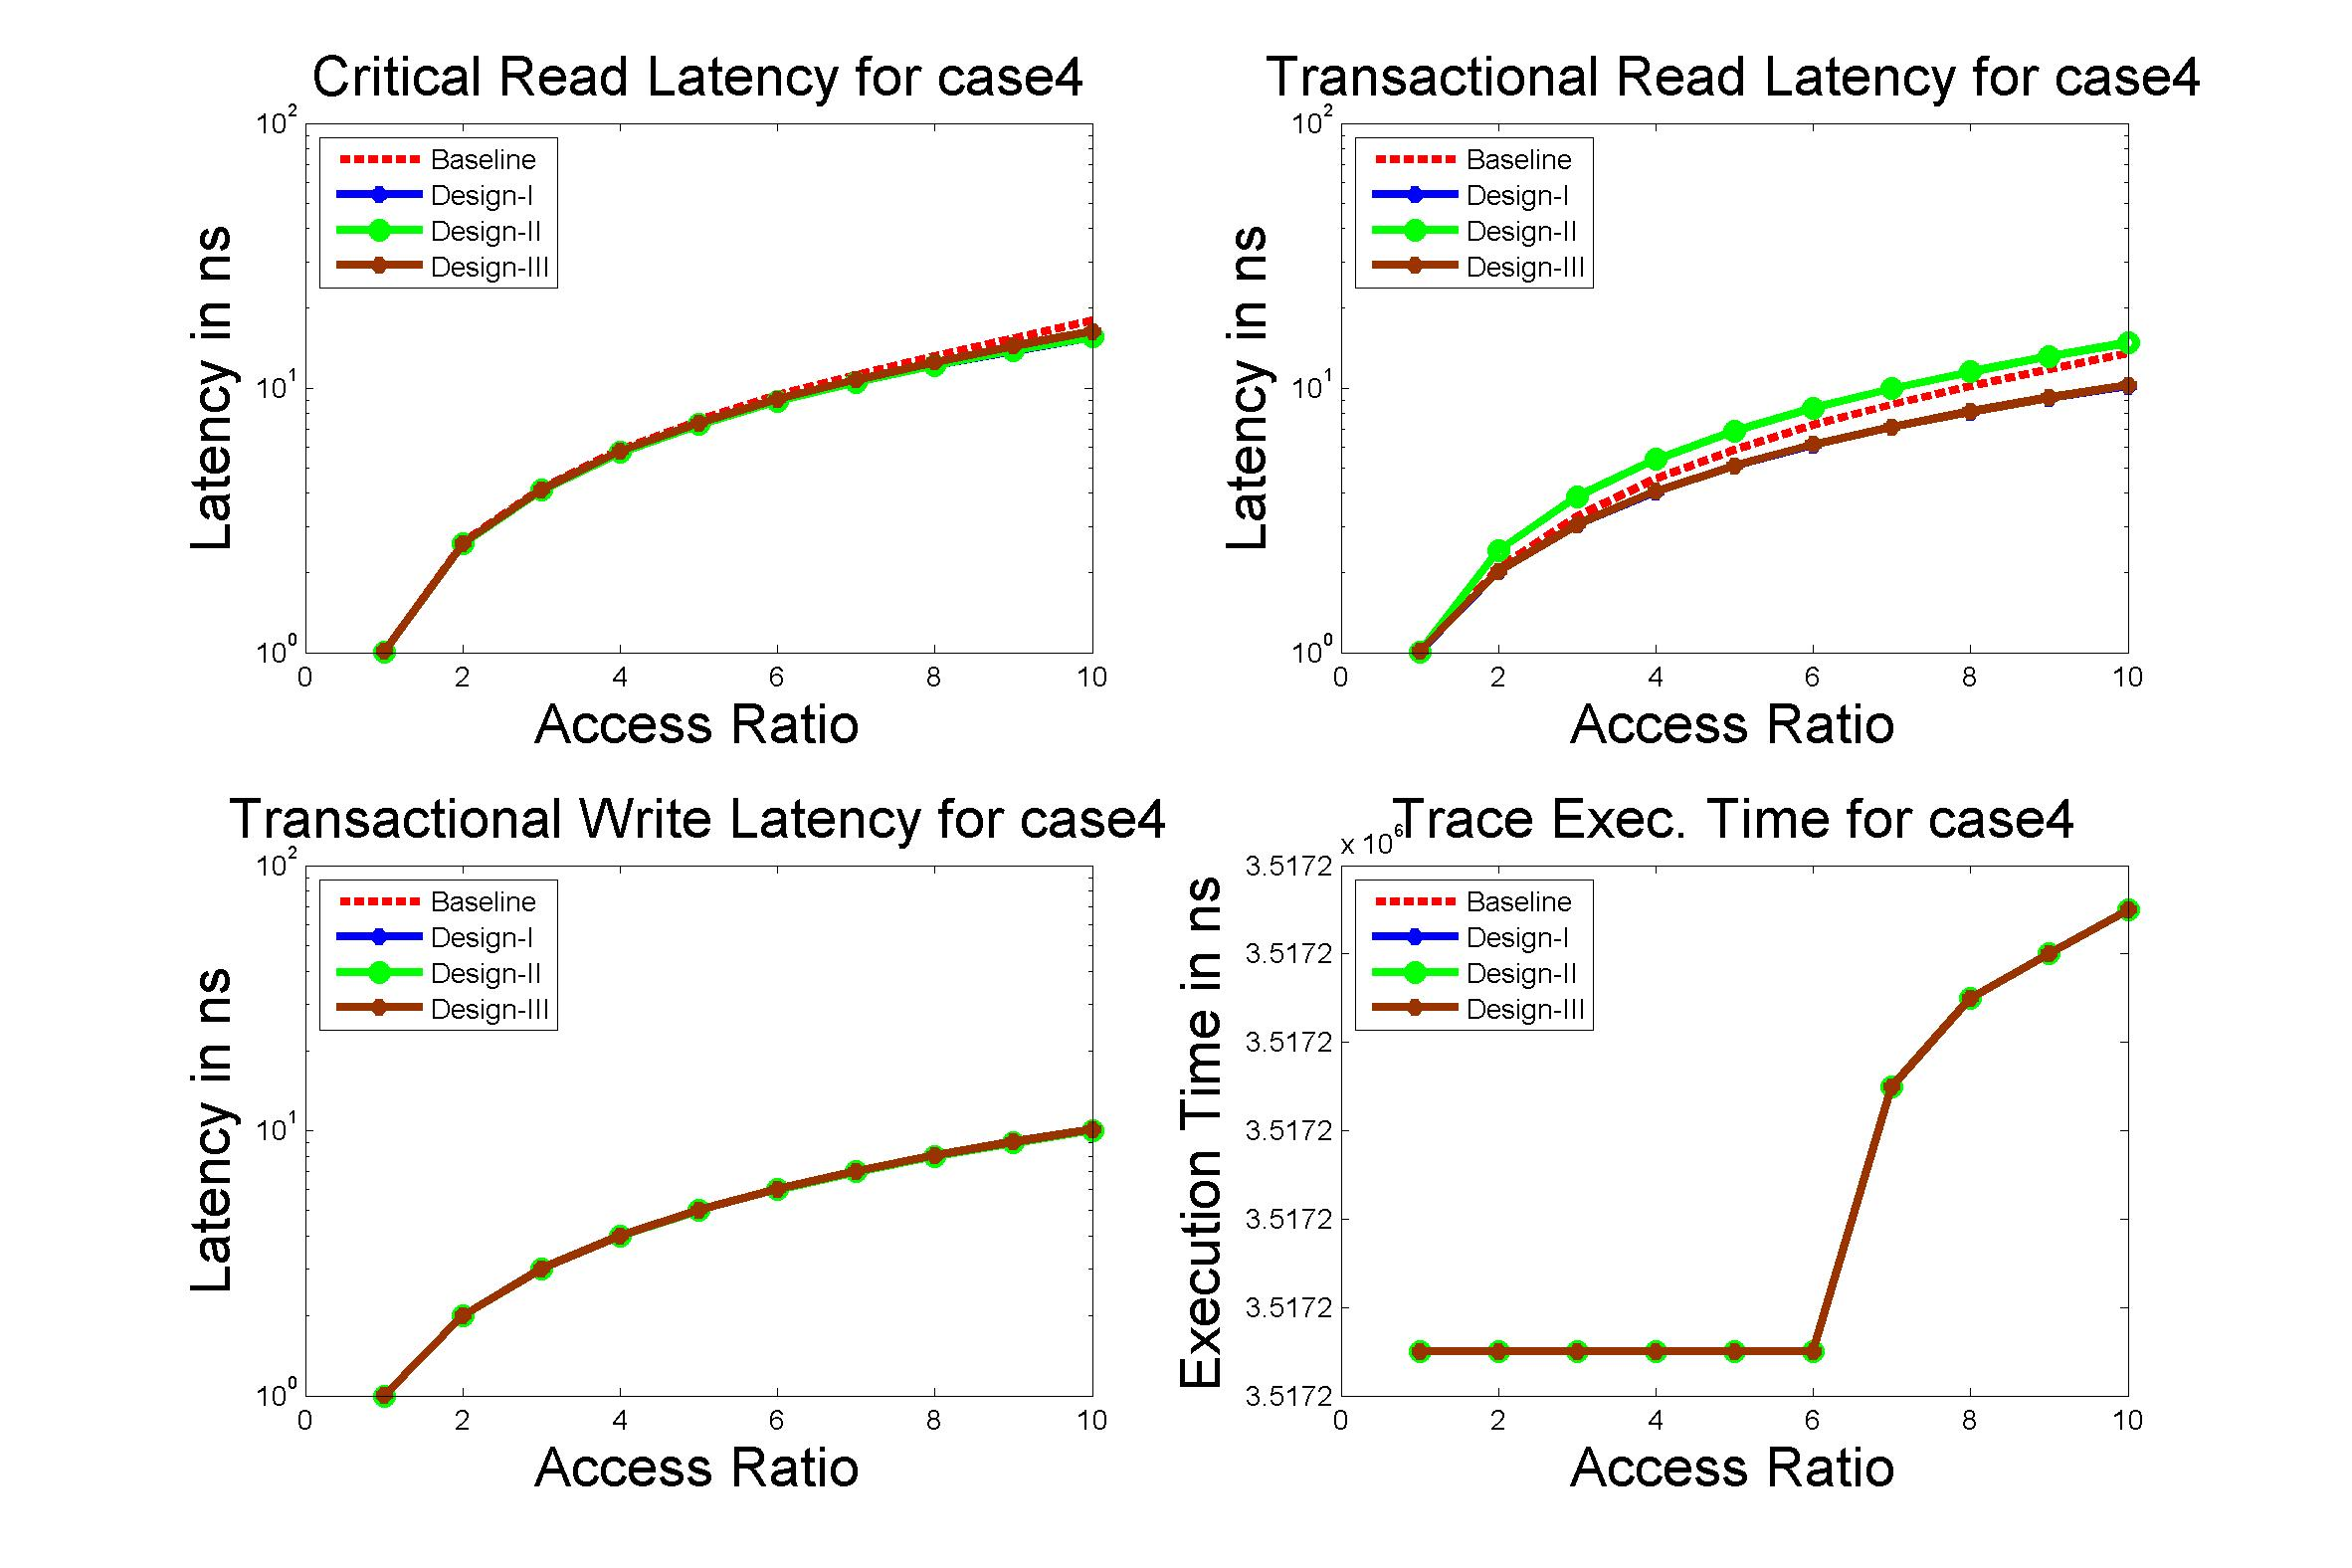
\includegraphics[width=\linewidth]{case4.jpg}
\end{minipage}
\caption{
{\bf Performance Graphs for case4 trace} }
\label{fig:case4}
\end{figure}
%-------------------------------------------------
\cleardoublepage
%-------------------------------------------------
\begin{figure}[htb]
\begin{minipage}[!t]{0.33\linewidth}
        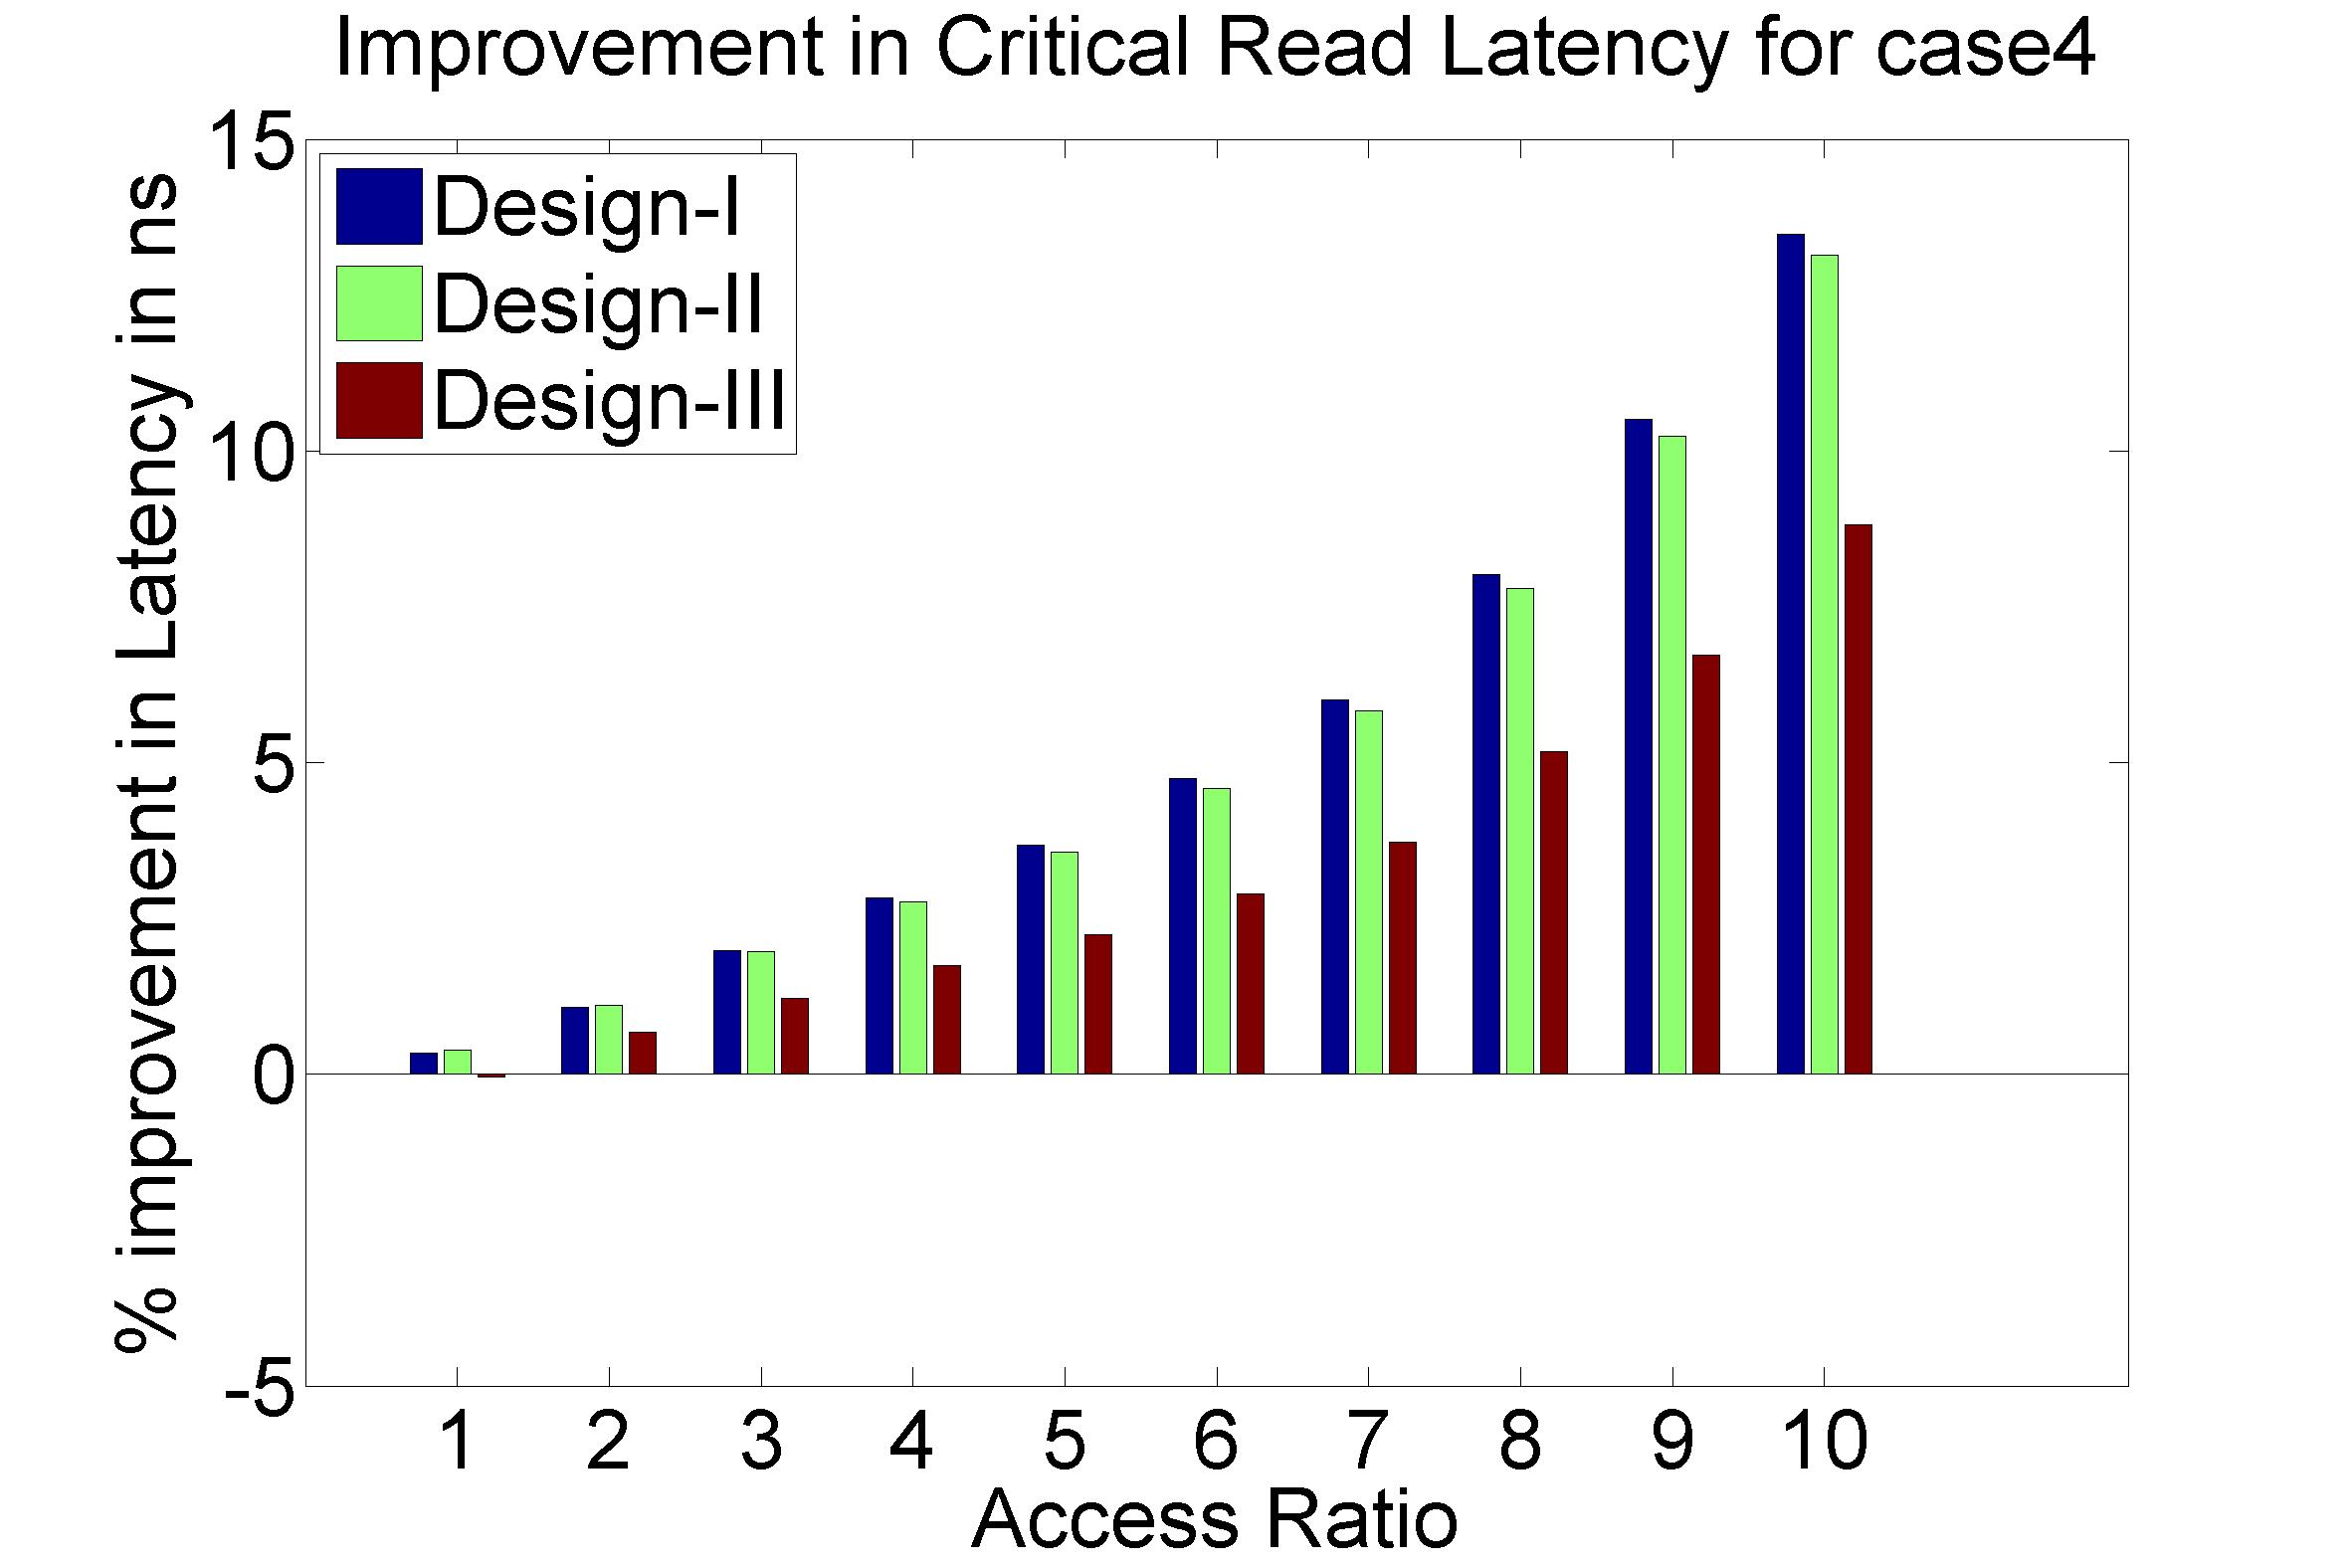
\includegraphics[width=\linewidth]{case4_critical_latency_improvement.jpeg}
\end{minipage}
\begin{minipage}[!t]{0.33\linewidth}
        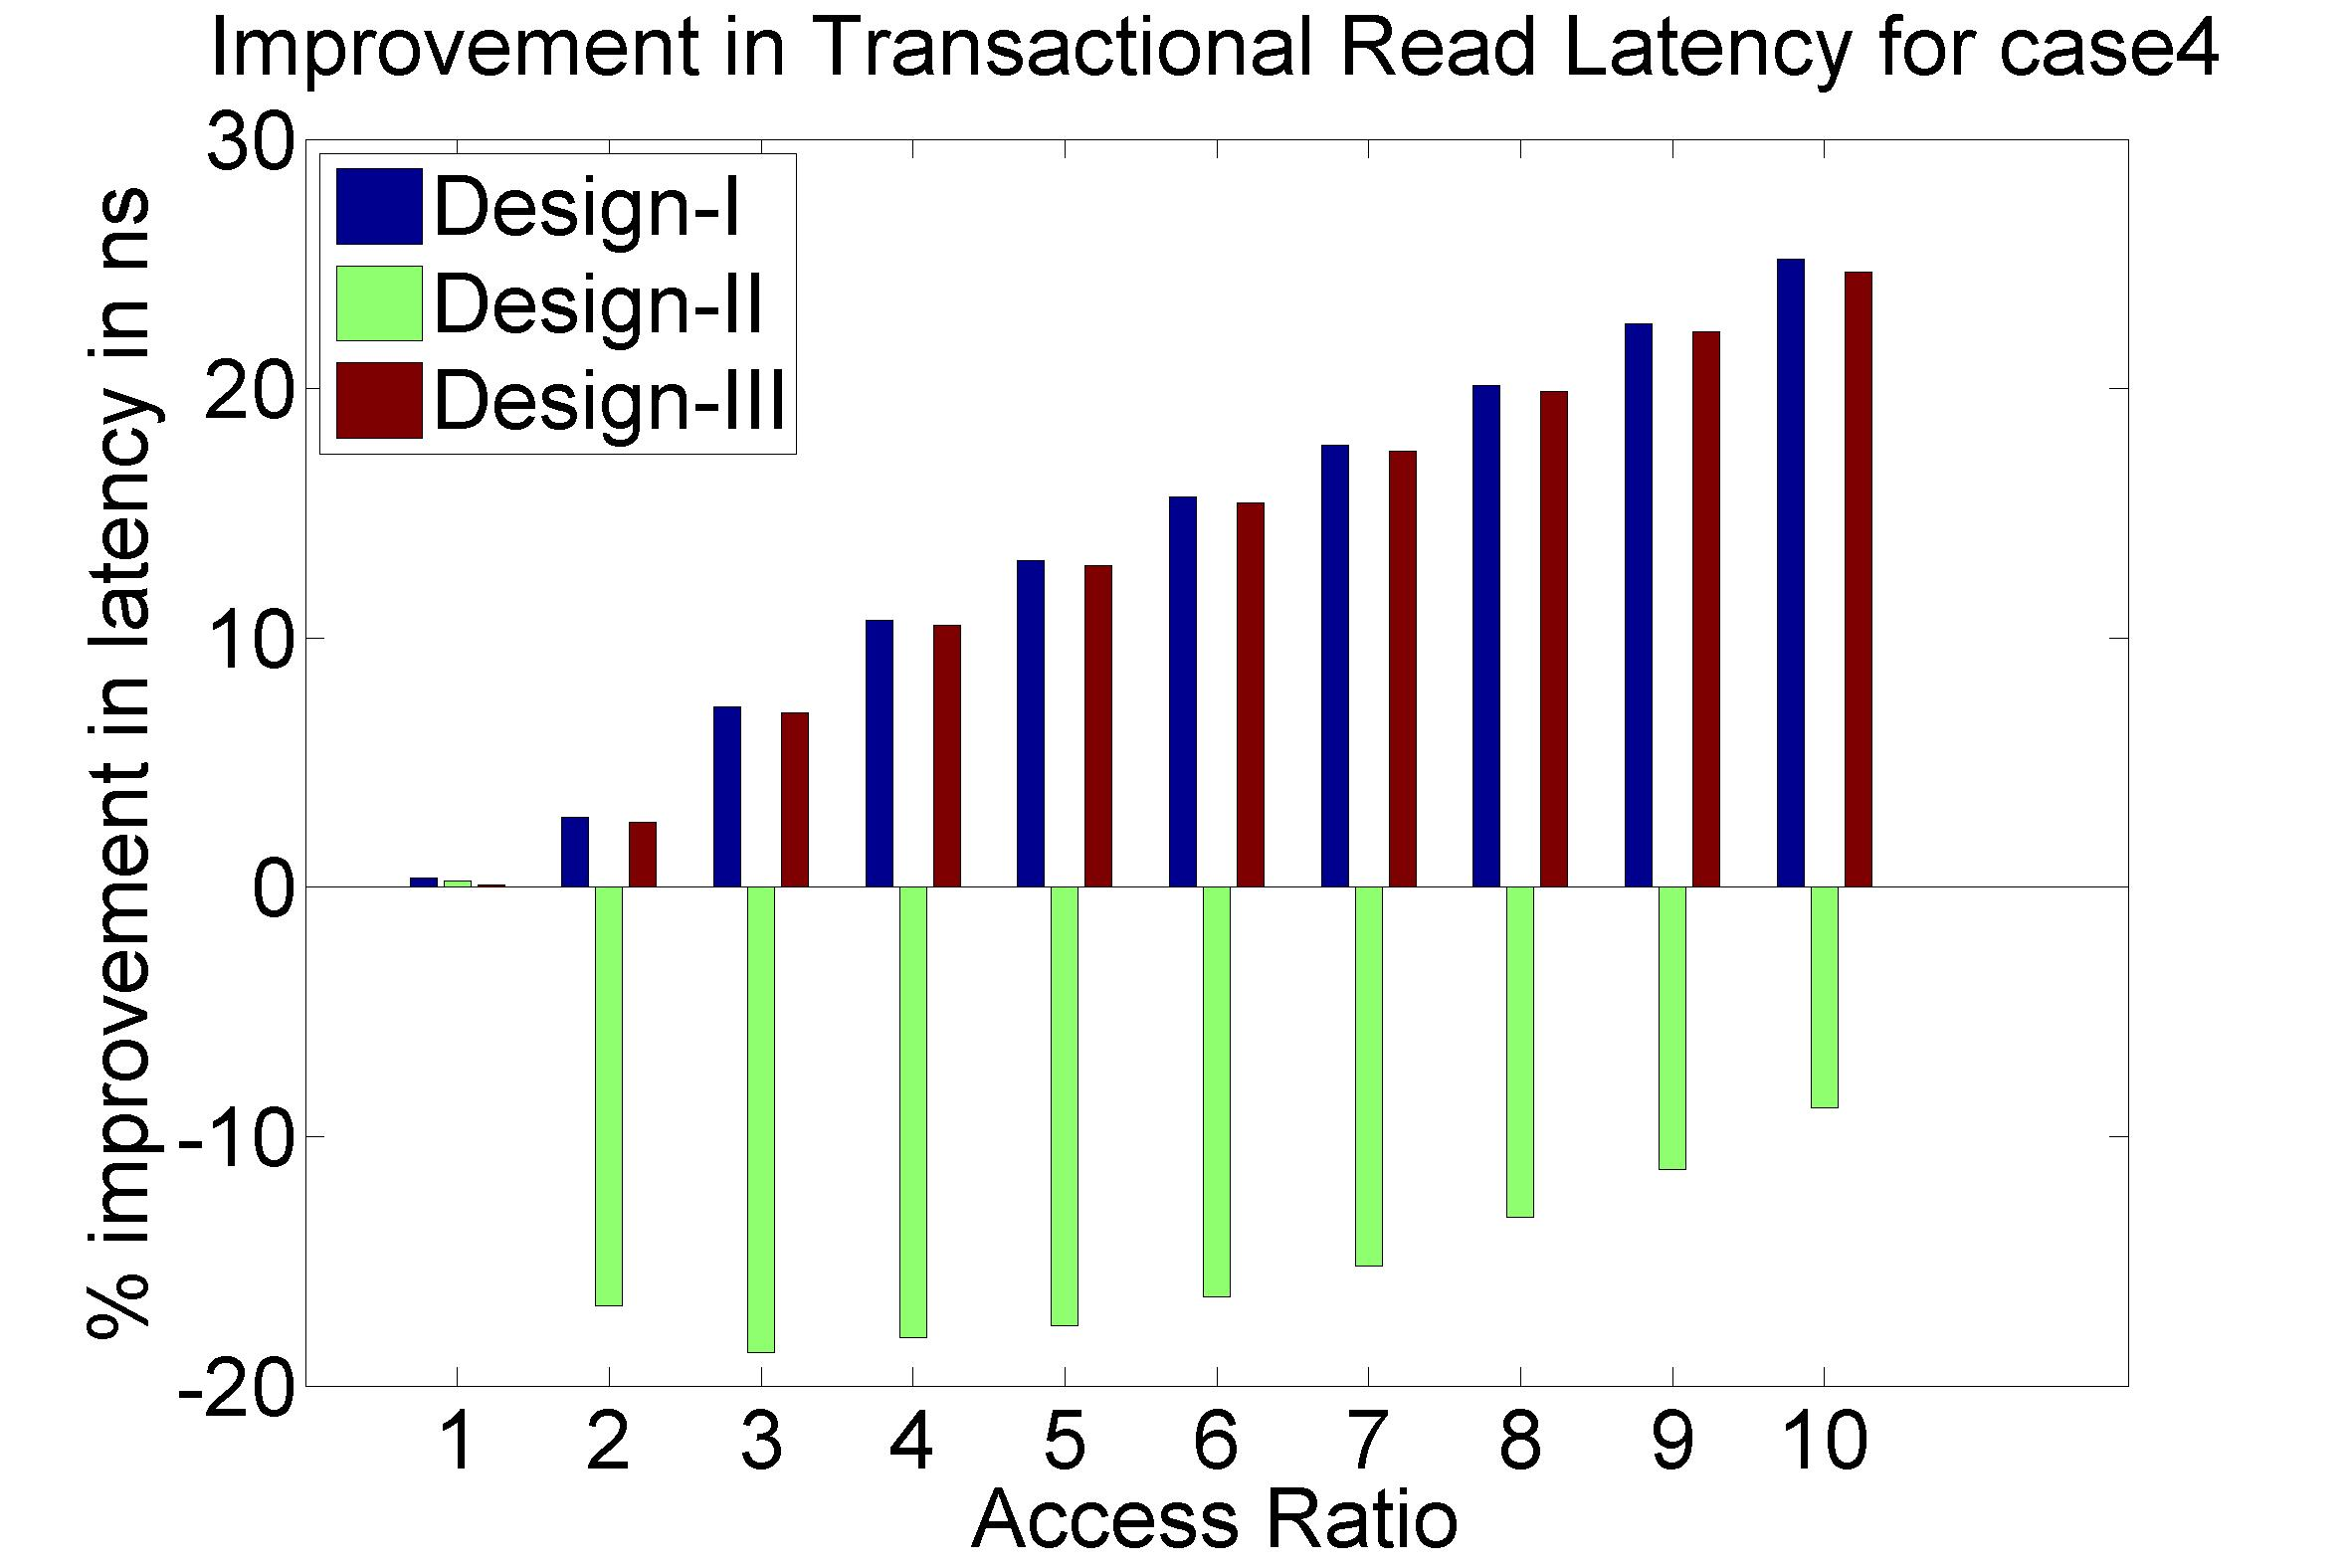
\includegraphics[width=\linewidth]{case4_transactional_latency_improvement.jpeg}
\end{minipage}
\begin{minipage}[!t]{0.33\linewidth}
        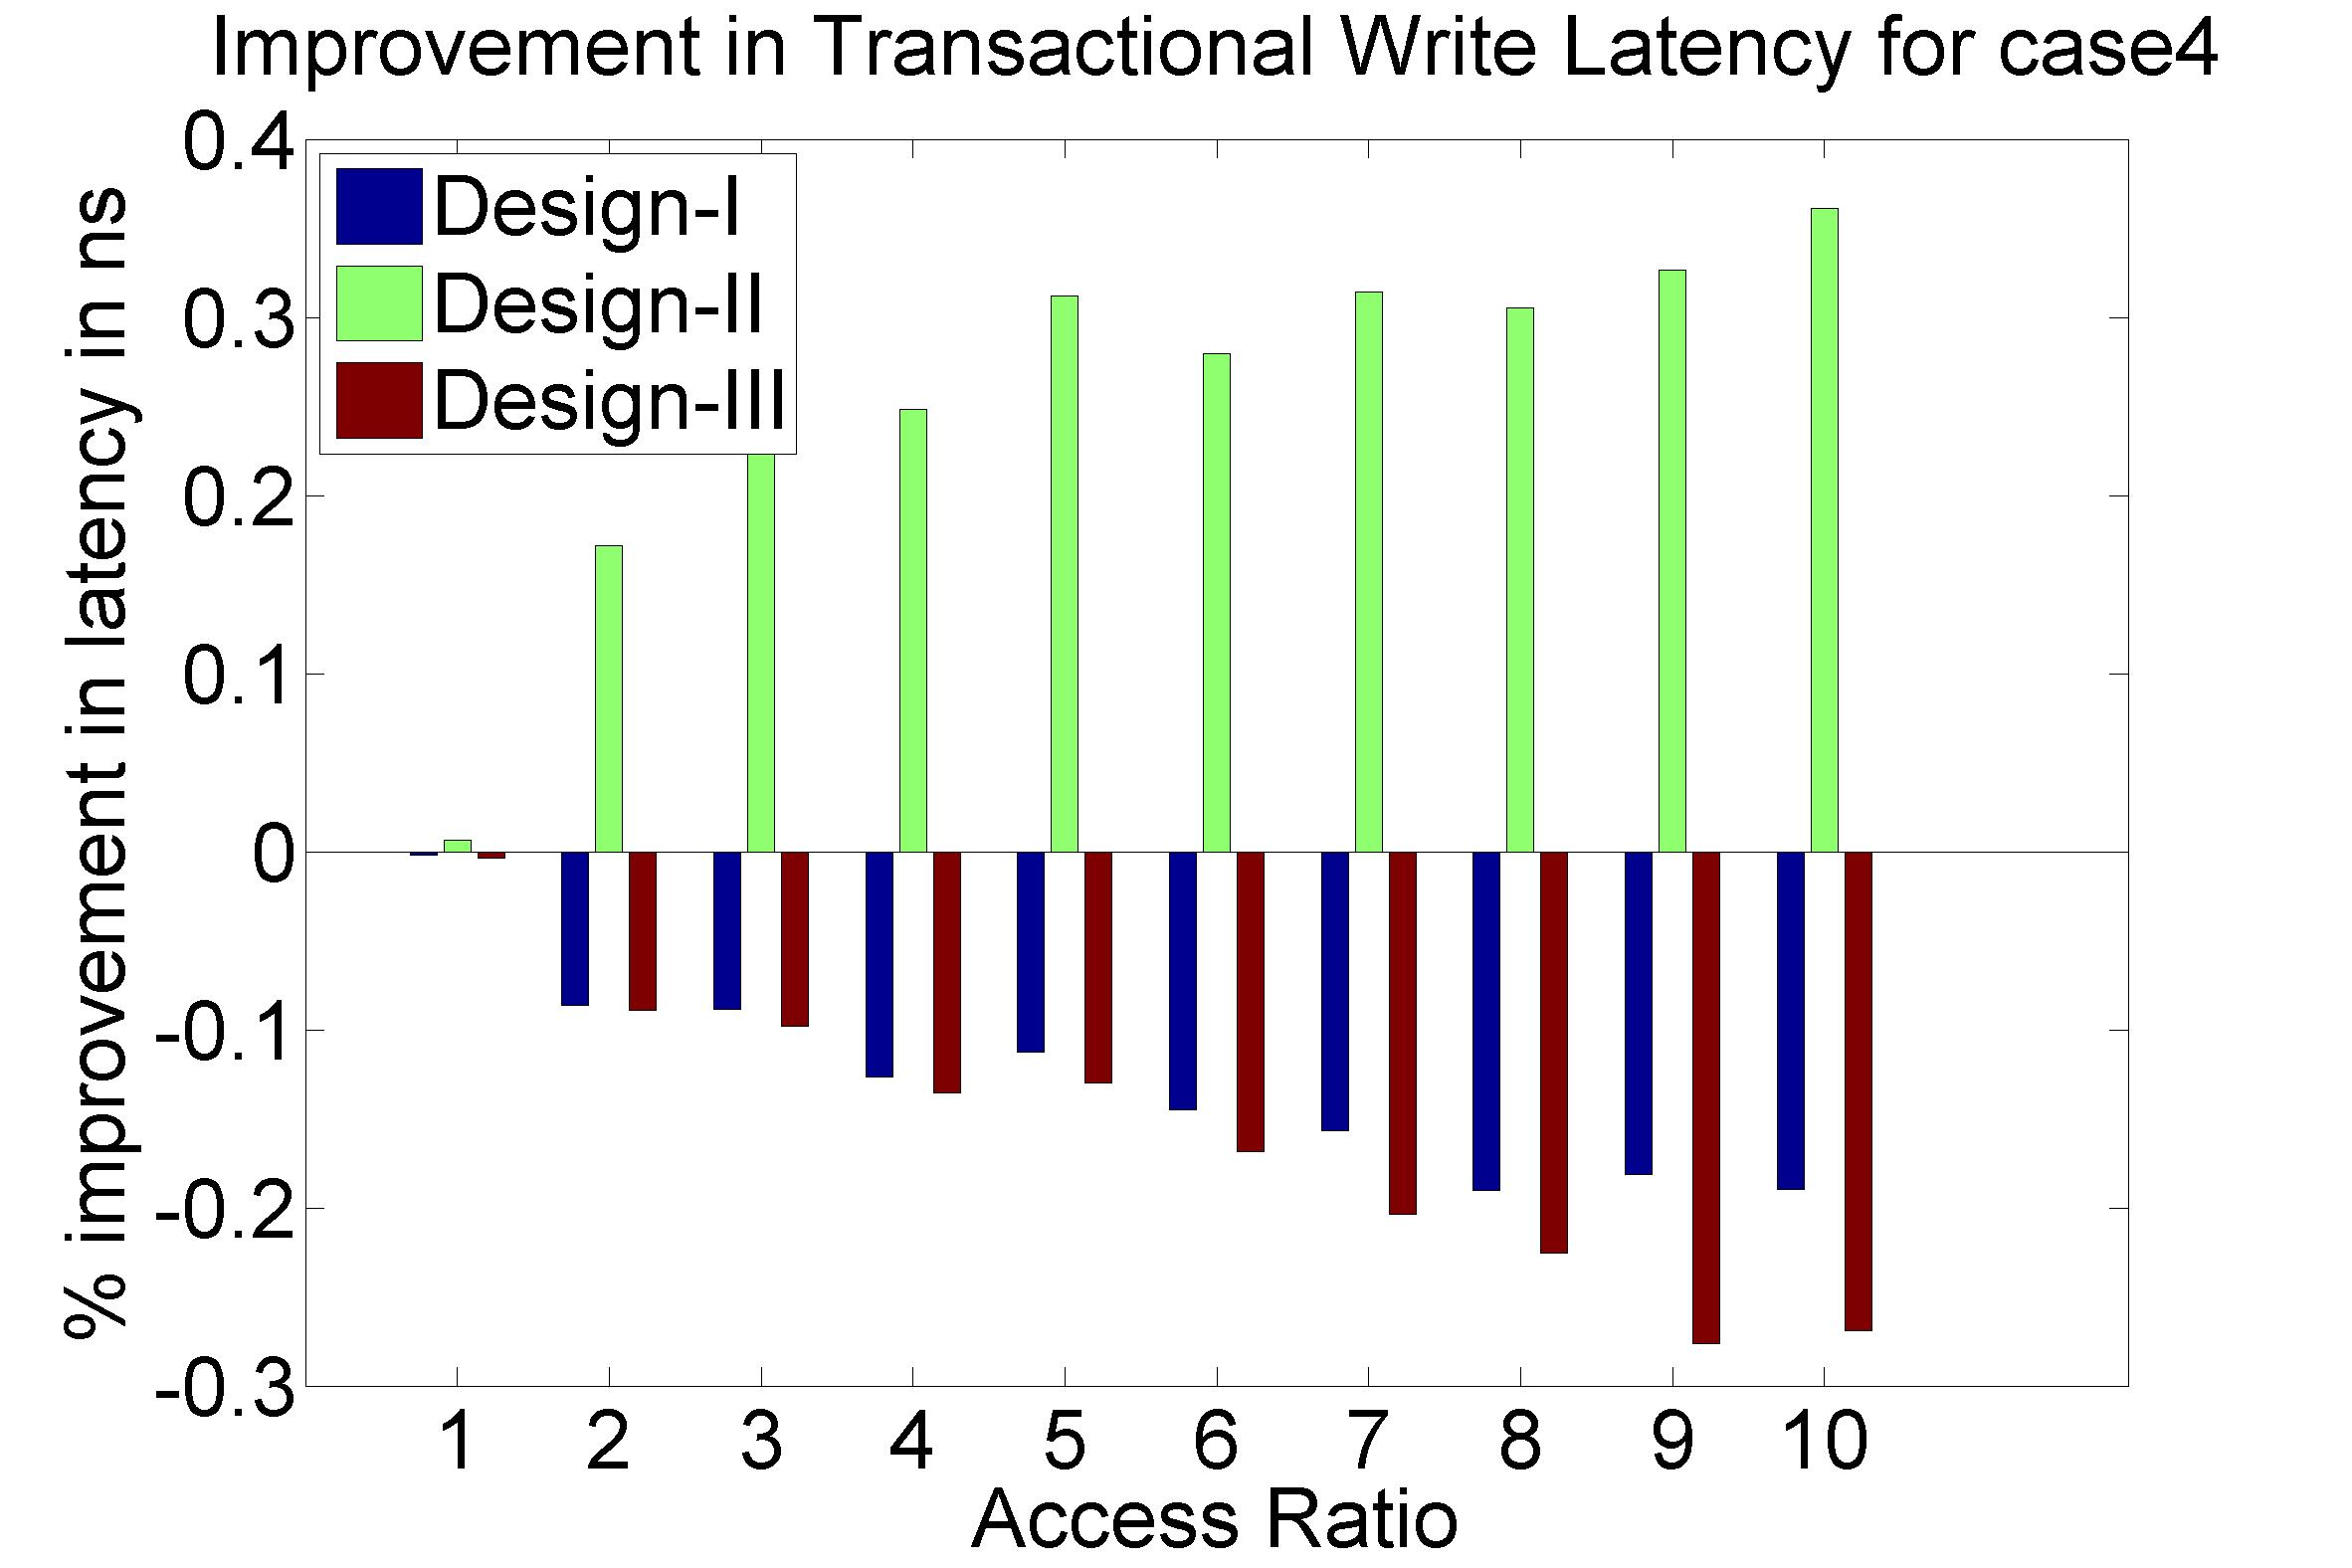
\includegraphics[width=\linewidth]{case4_write_latency_improvement.jpeg}
\end{minipage}
\caption{
{\bf Performance Graphs for case4 trace} }
\label{fig:case4_improvement}
\end{figure}
%-------------------------------------------------
Observations:
\begin{itemize}
	\item The case4 traces are low density traces. That is, the number of access requests per time period are low. 
	\item The Critical Read latency improvement in {\em positive} for all the ratios. 
	\item The critical read latency exponentially improves for increased access ratios.
	\item The transactional Read latency also improves for design I and design III. 
	\item The write latency has only marginal improvement. 
	\item The results suggest that in case4, we do not use the "coding" aspect due to low density access in case of Writes.
	\item The improvement in Transactional Read Latency is substantial. 
\end{itemize}
\cleardoublepage
%-------------------------------------------------
\begin{figure}[htb]
\begin{minipage}[!t]{\linewidth}
        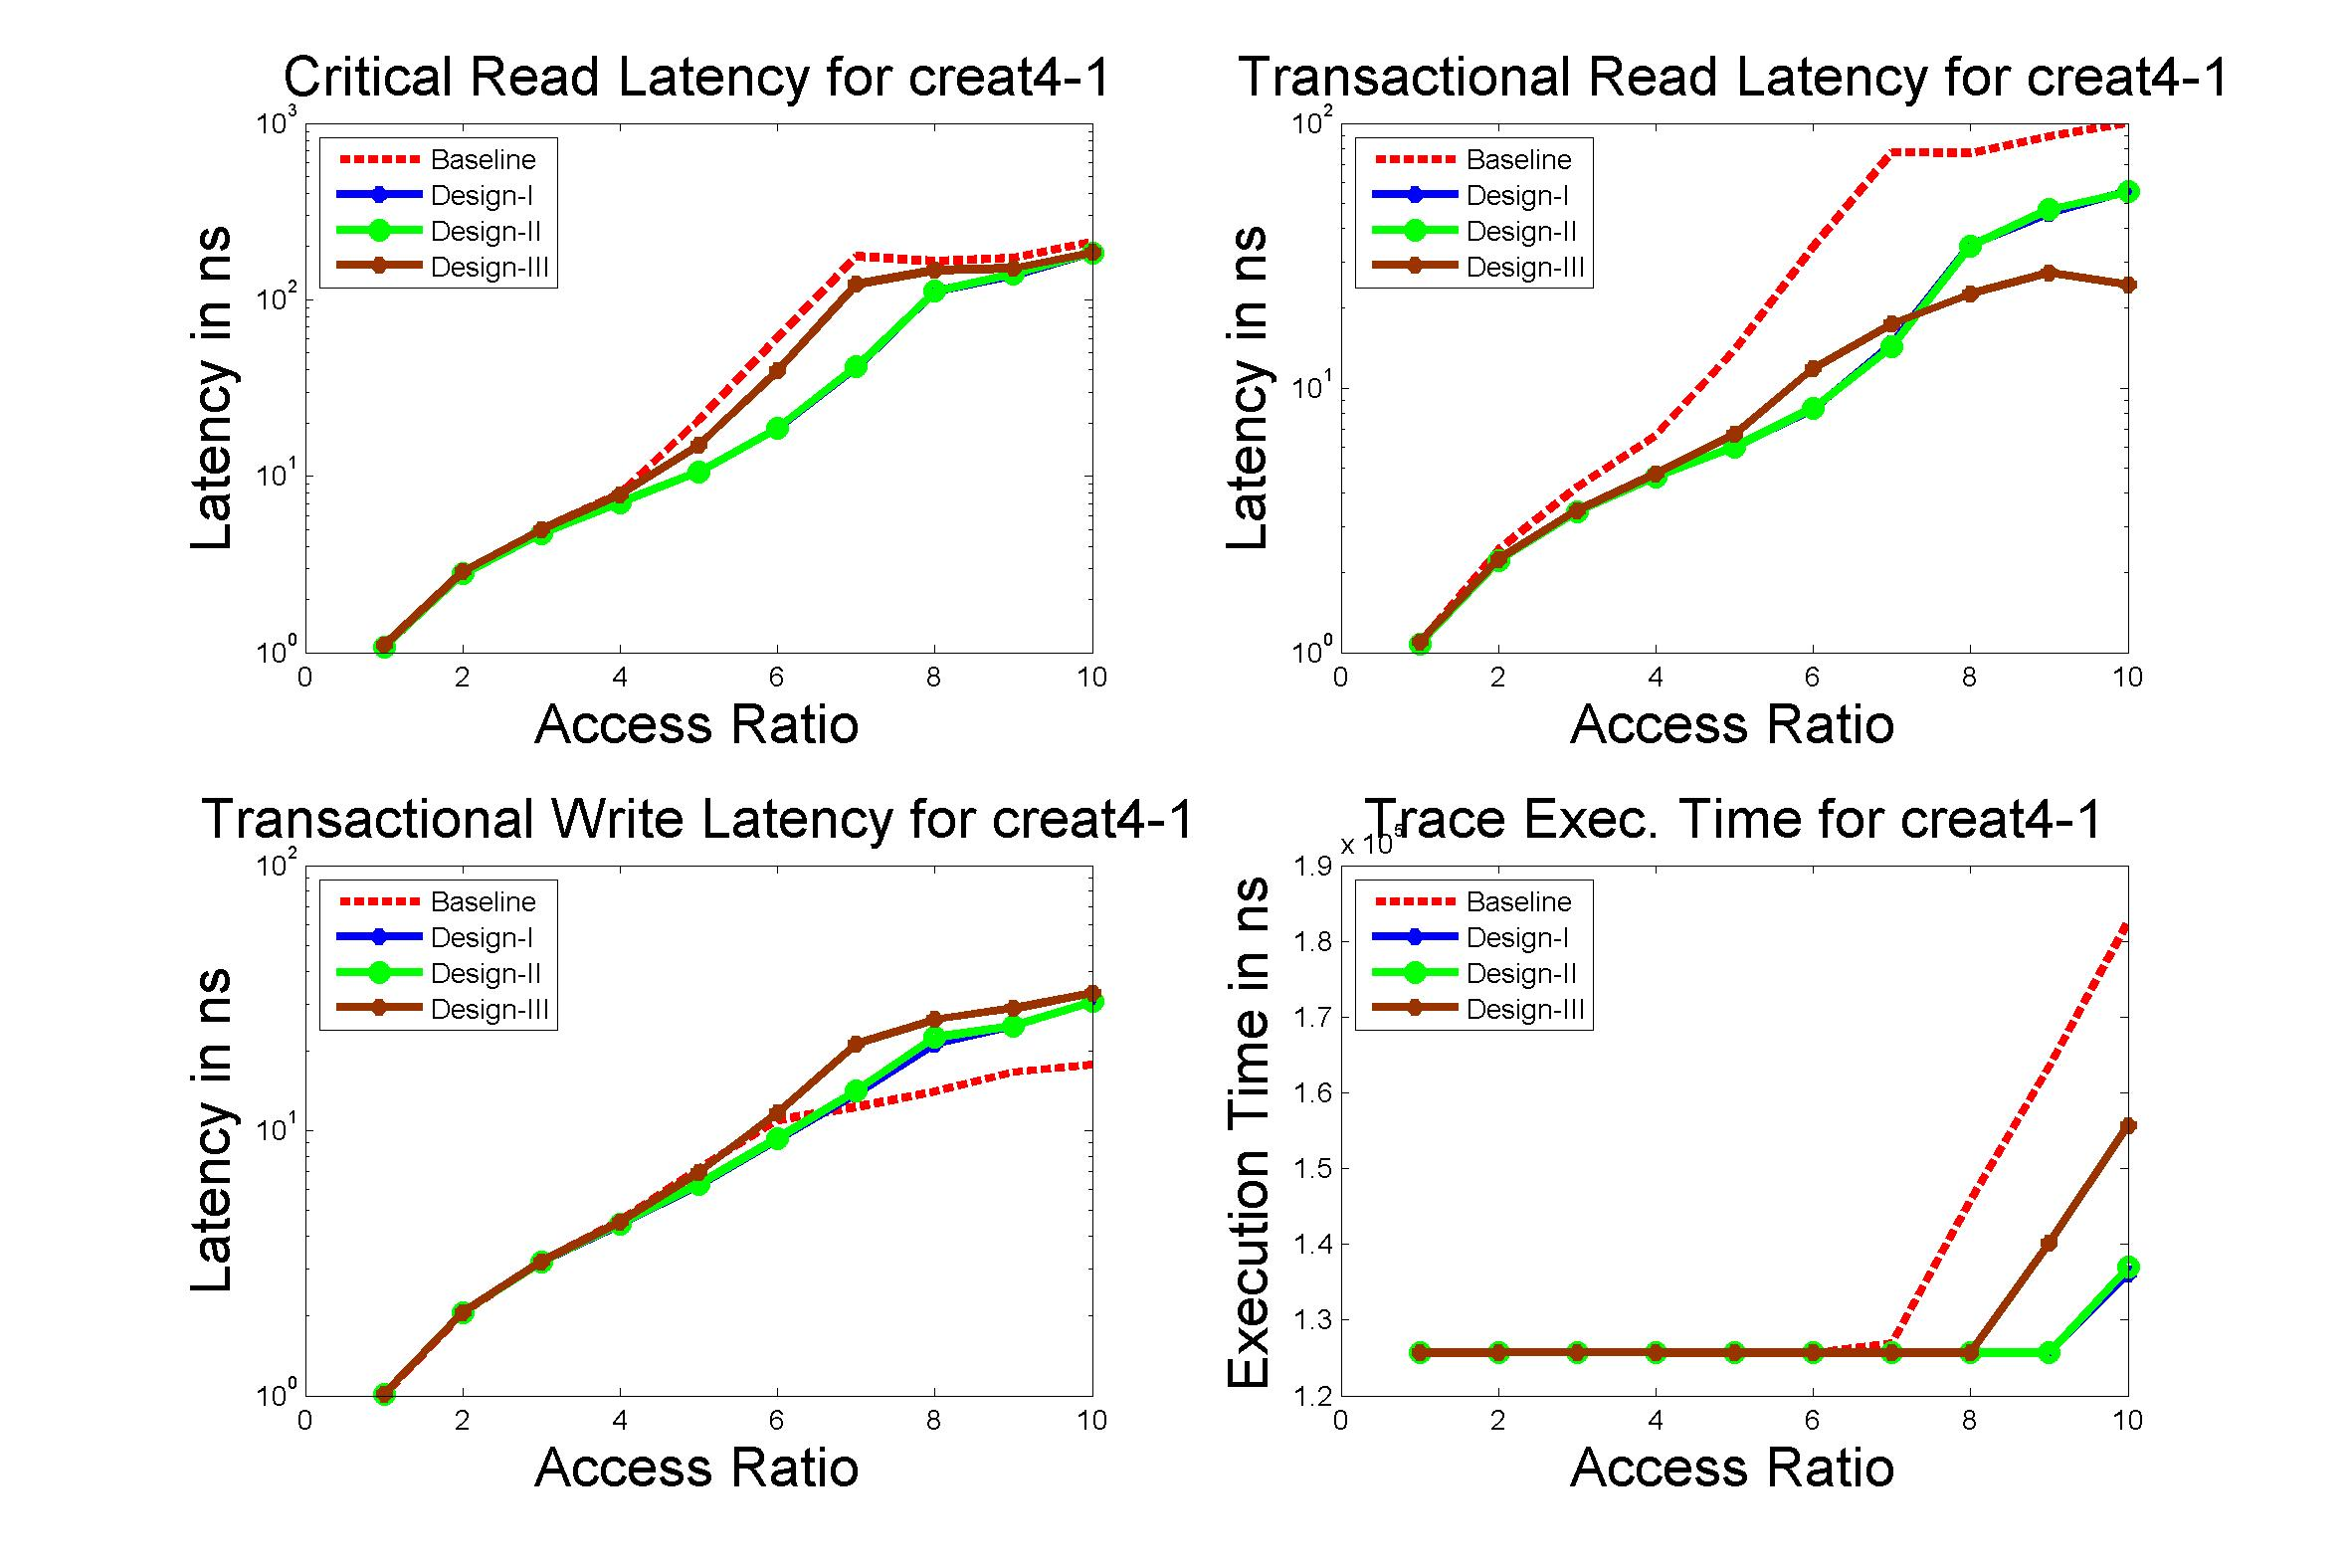
\includegraphics[width=\linewidth]{creat4-1.jpg}
\end{minipage}
\caption{
{\bf Performance Graphs for Creat4-1 trace} }
\label{fig:creat41}
\end{figure}
%-------------------------------------------------
\cleardoublepage
%-------------------------------------------------
\begin{figure}[htb]
\begin{minipage}[!t]{0.33\linewidth}
        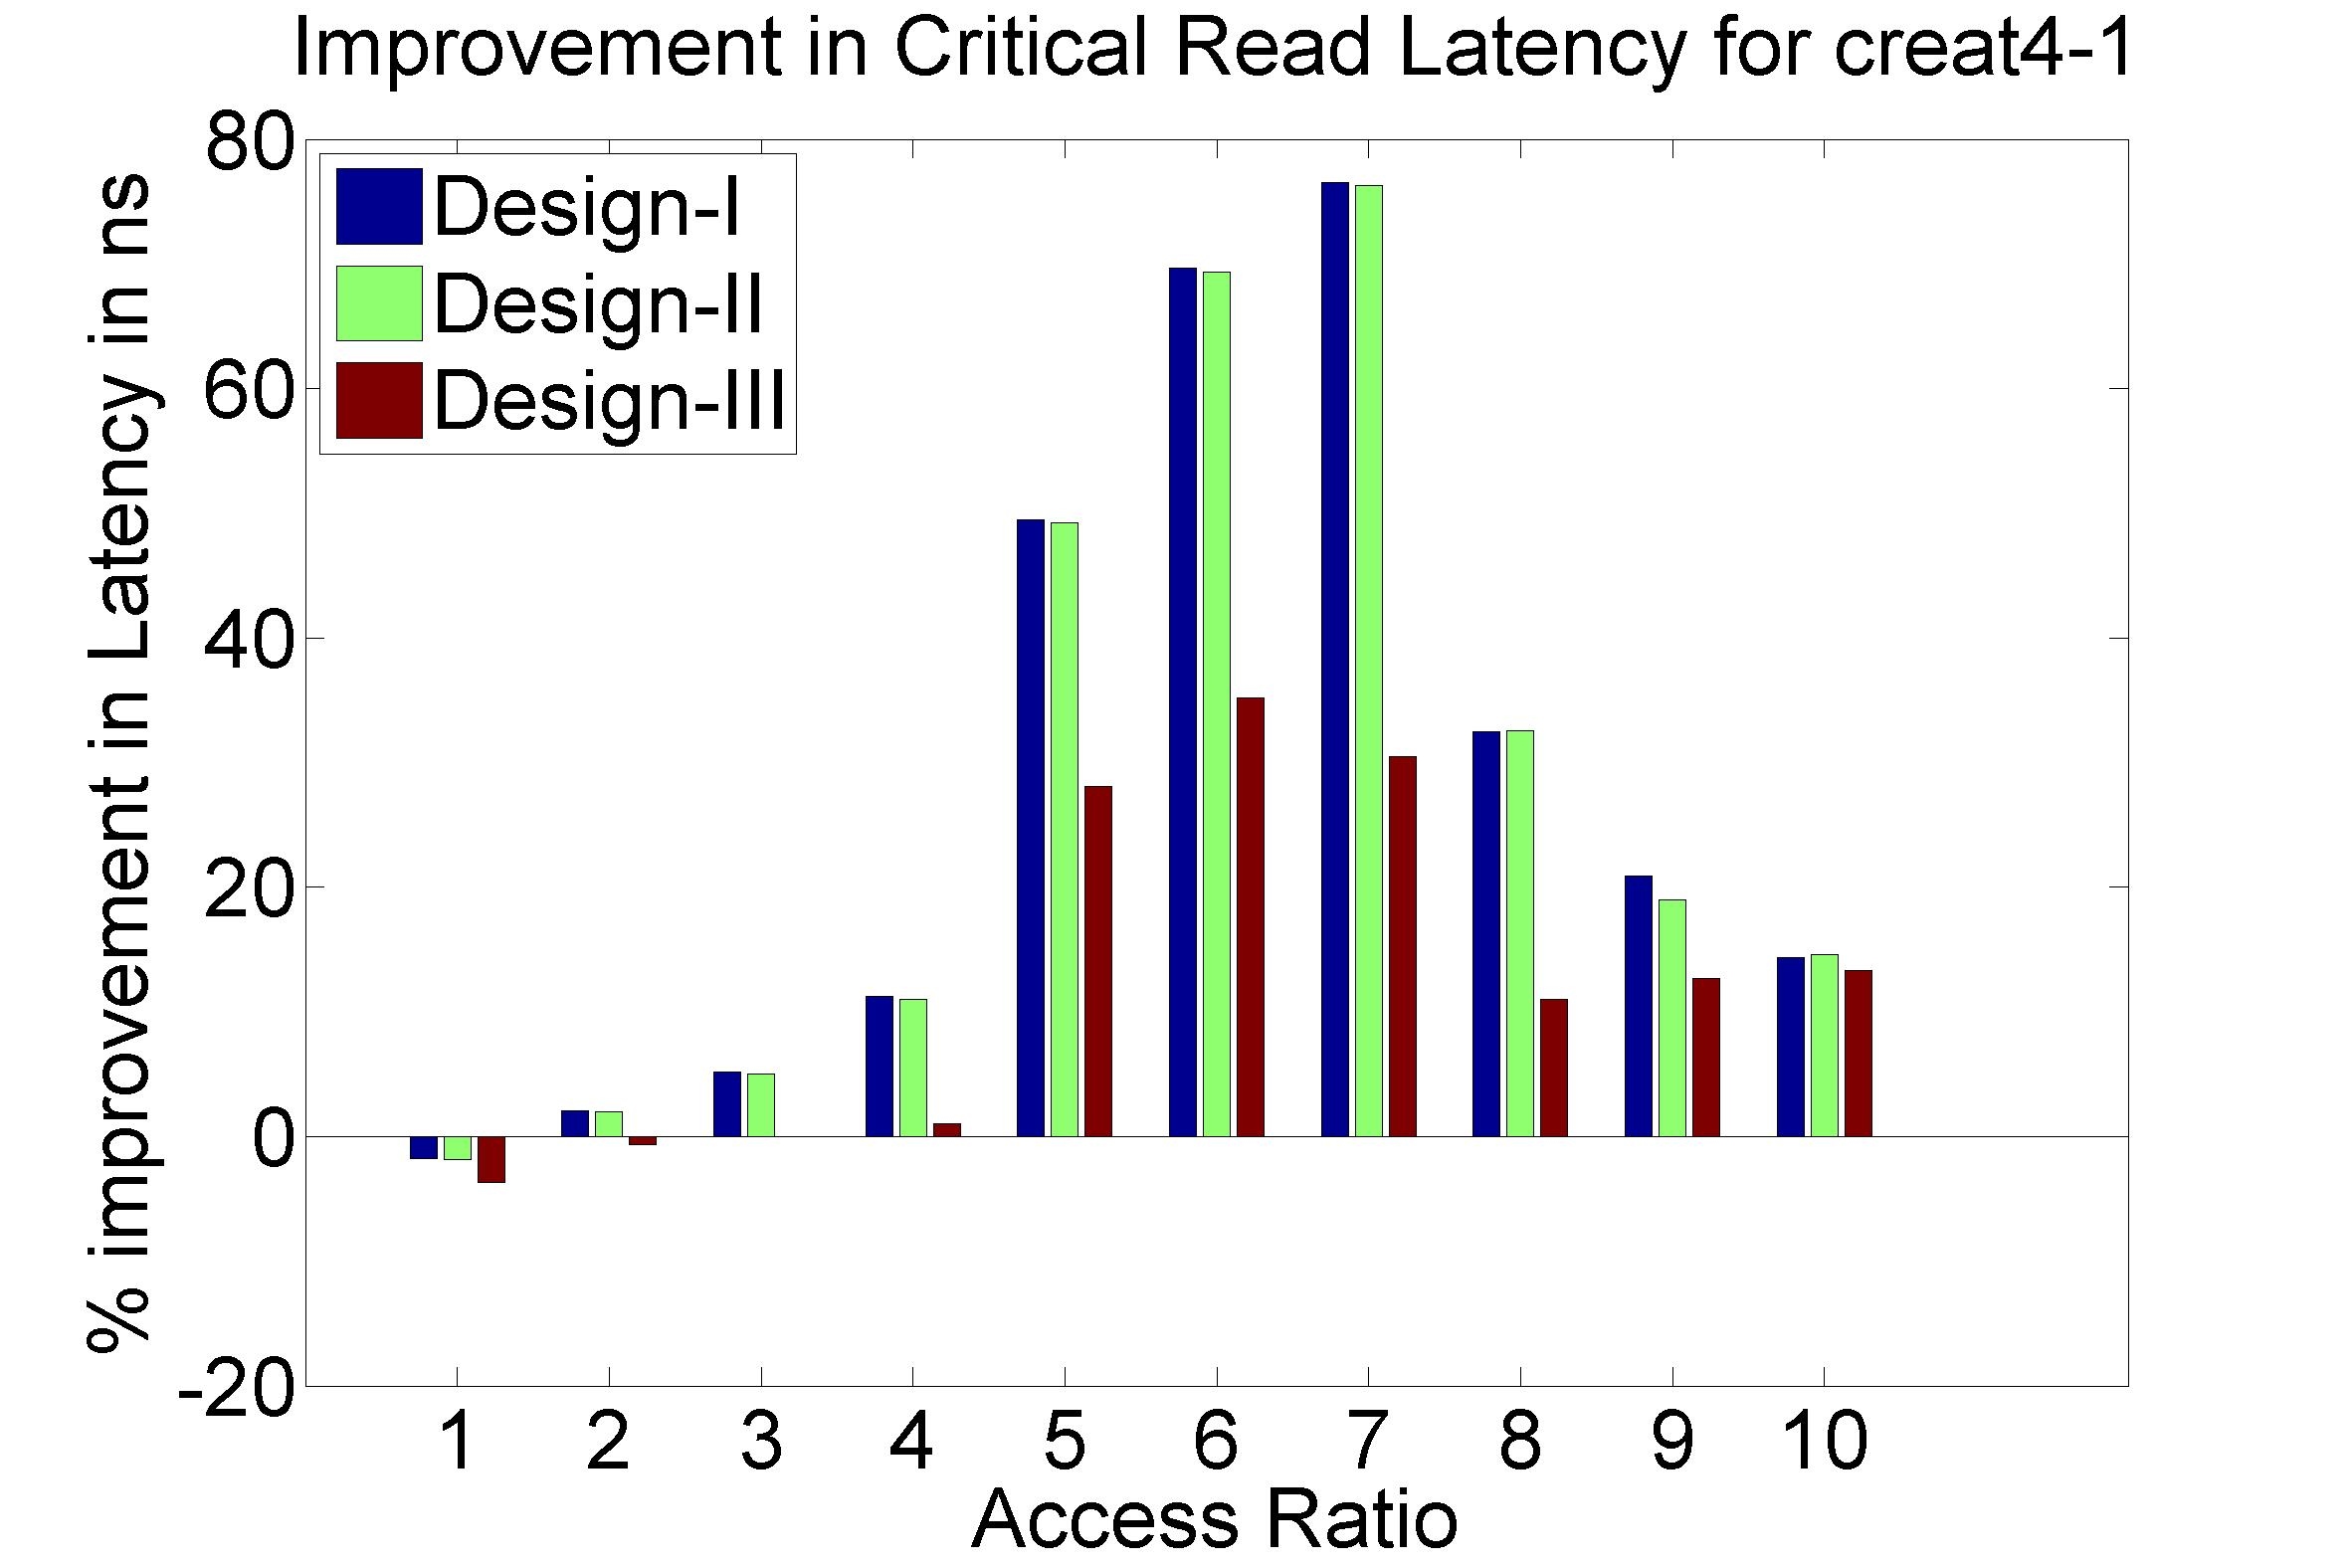
\includegraphics[width=\linewidth]{creat4-1_critical_latency_improvement.jpeg}
\end{minipage}
\begin{minipage}[!t]{0.33\linewidth}
        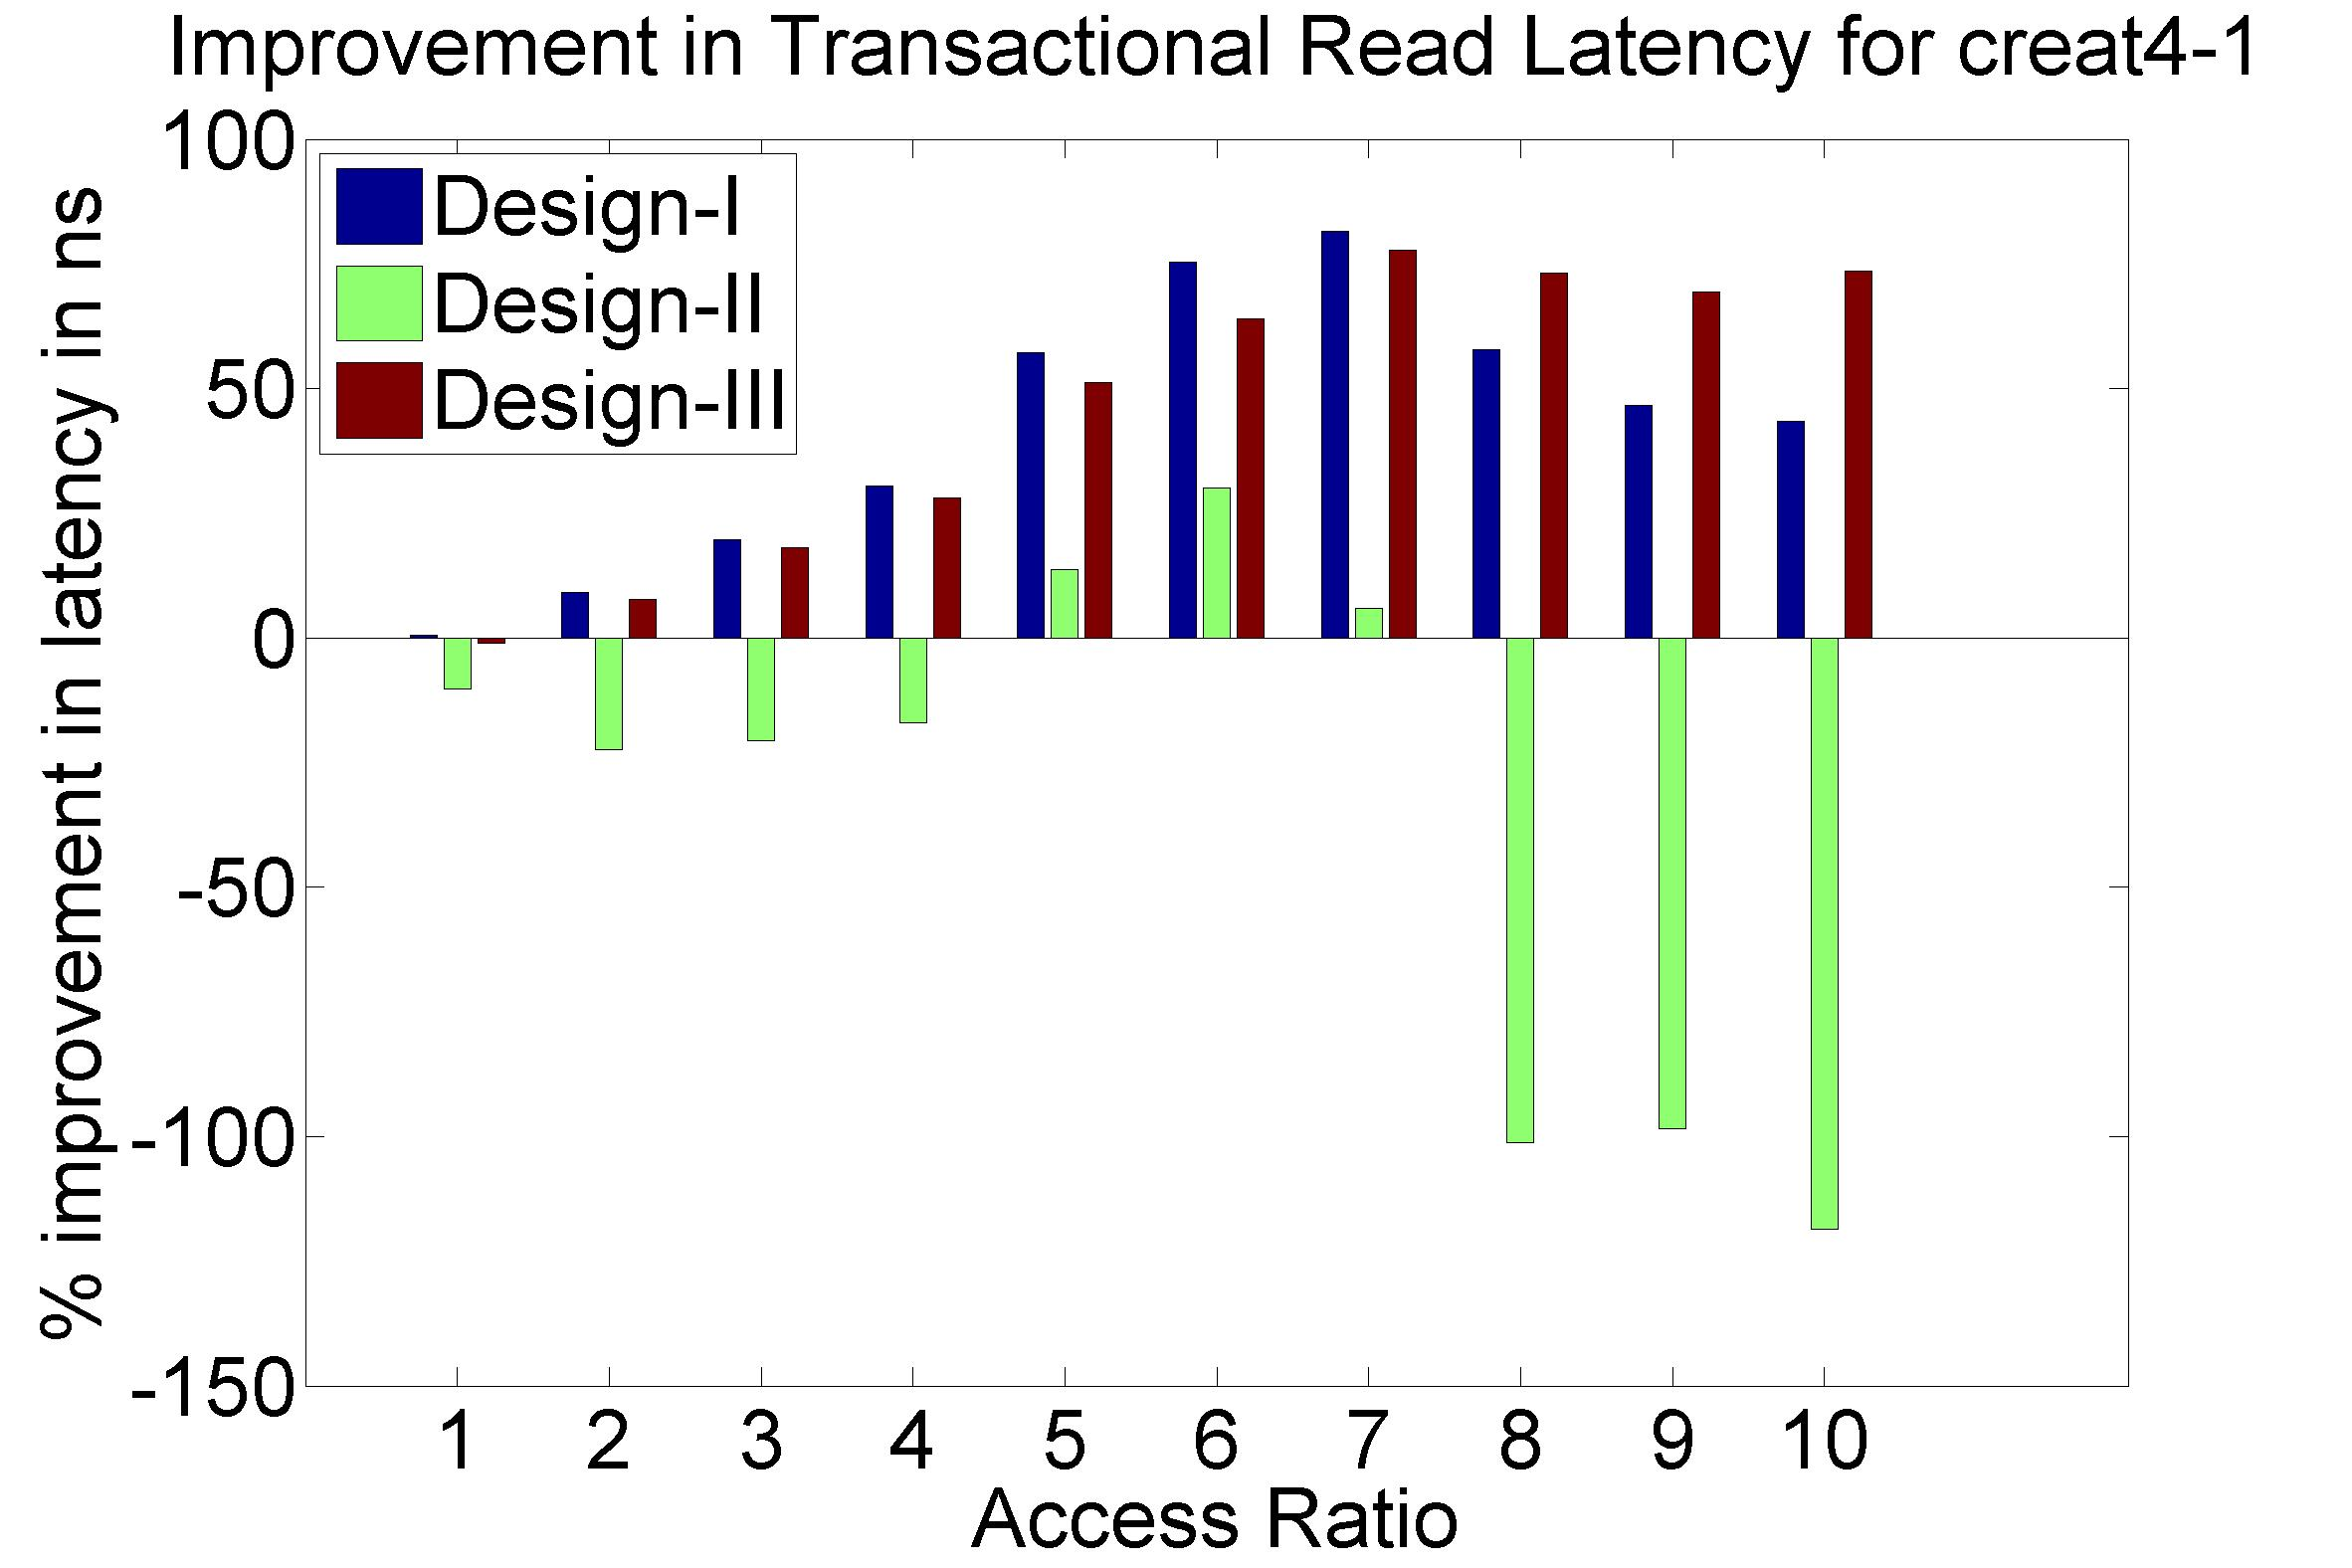
\includegraphics[width=\linewidth]{creat4-1_transactional_latency_improvement.jpeg}
\end{minipage}
\begin{minipage}[!t]{0.33\linewidth}
        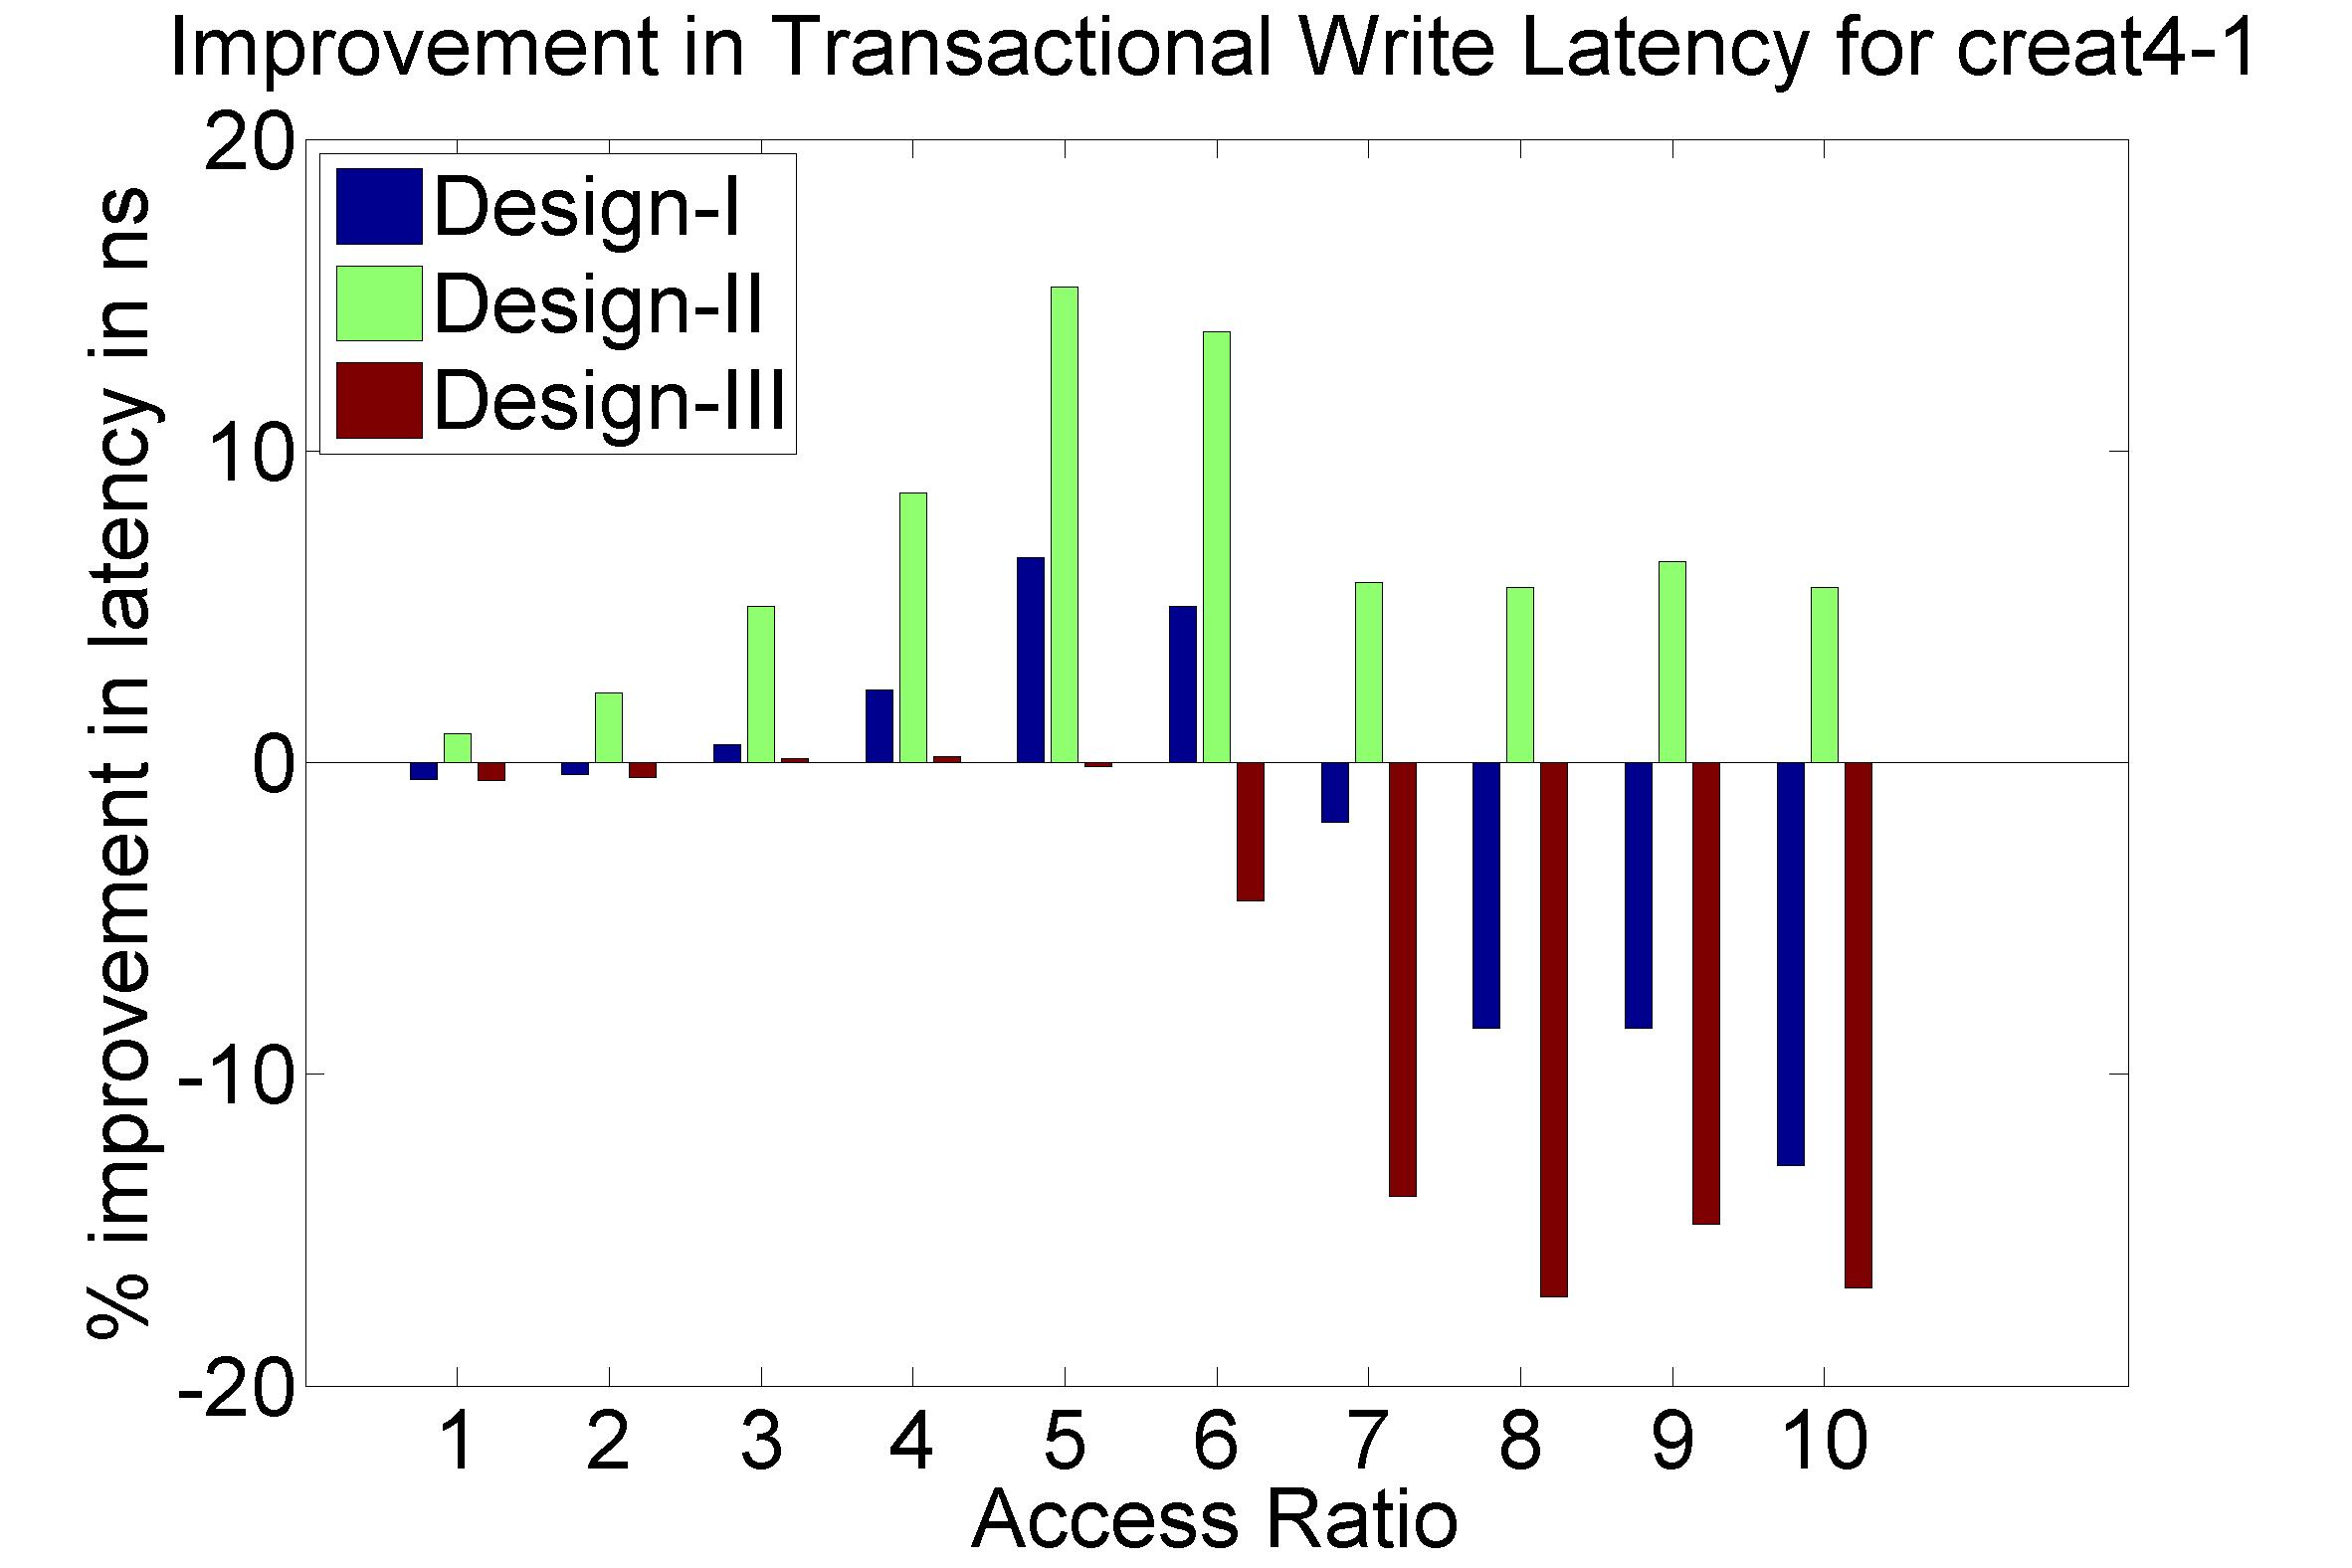
\includegraphics[width=\linewidth]{creat4-1_write_latency_improvement.jpeg}
\end{minipage}
\caption{
{\bf Performance Graphs for Creat4-1 trace} }
\label{fig:creat41_improvement}
\end{figure}
%-------------------------------------------------
Observations:
\begin{itemize}
	\item The trace creat4-1 is a medium density trace. 
	\item The improvement in critical read latency and transactional read latency is significant in design I and design II. 
	\item The write latency is positive till access ratio of 6.
	\item Design I and Design III codes benefit in this trace.
\end{itemize}
\cleardoublepage
%-------------------------------------------------
\begin{figure}[htb]
\begin{minipage}[!t]{\linewidth}
        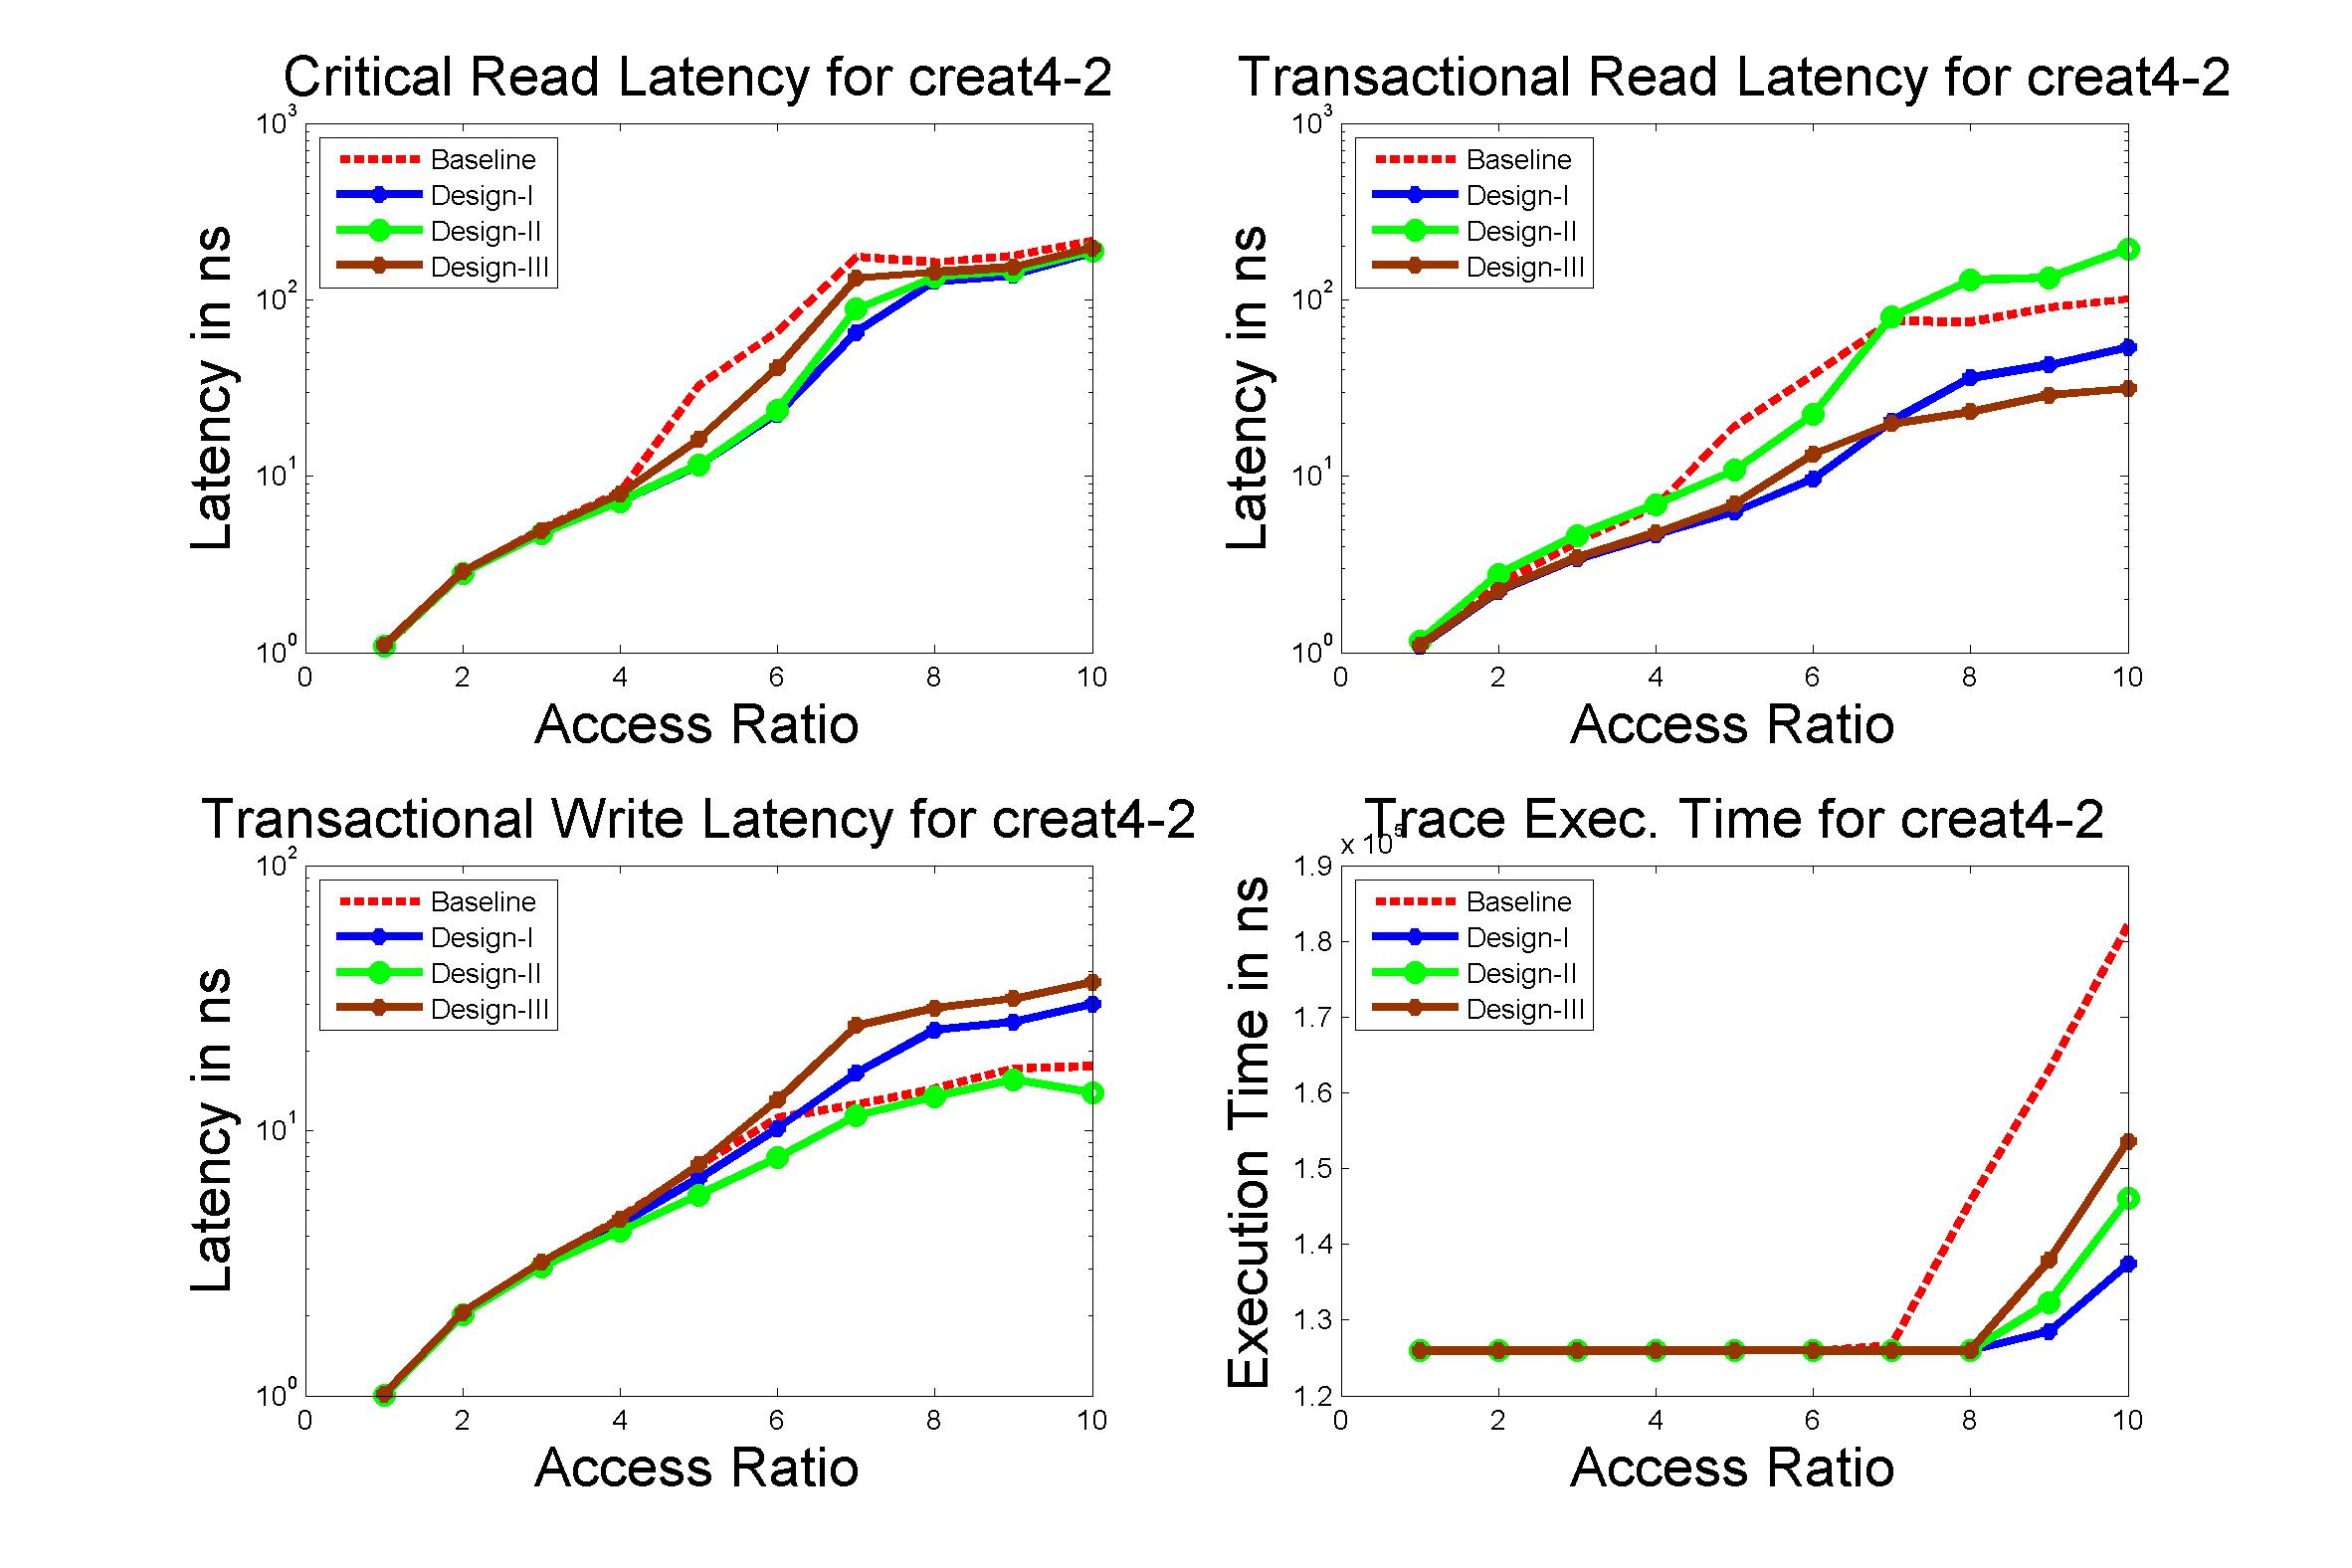
\includegraphics[width=\linewidth]{creat4-2.jpg}
\end{minipage}
\caption{
{\bf Performance Graphs for Creat4-2 trace} }
\label{fig:creat42}
\end{figure}
%-------------------------------------------------
\cleardoublepage
%-------------------------------------------------
\begin{figure}[htb]
\begin{minipage}[!t]{0.33\linewidth}
        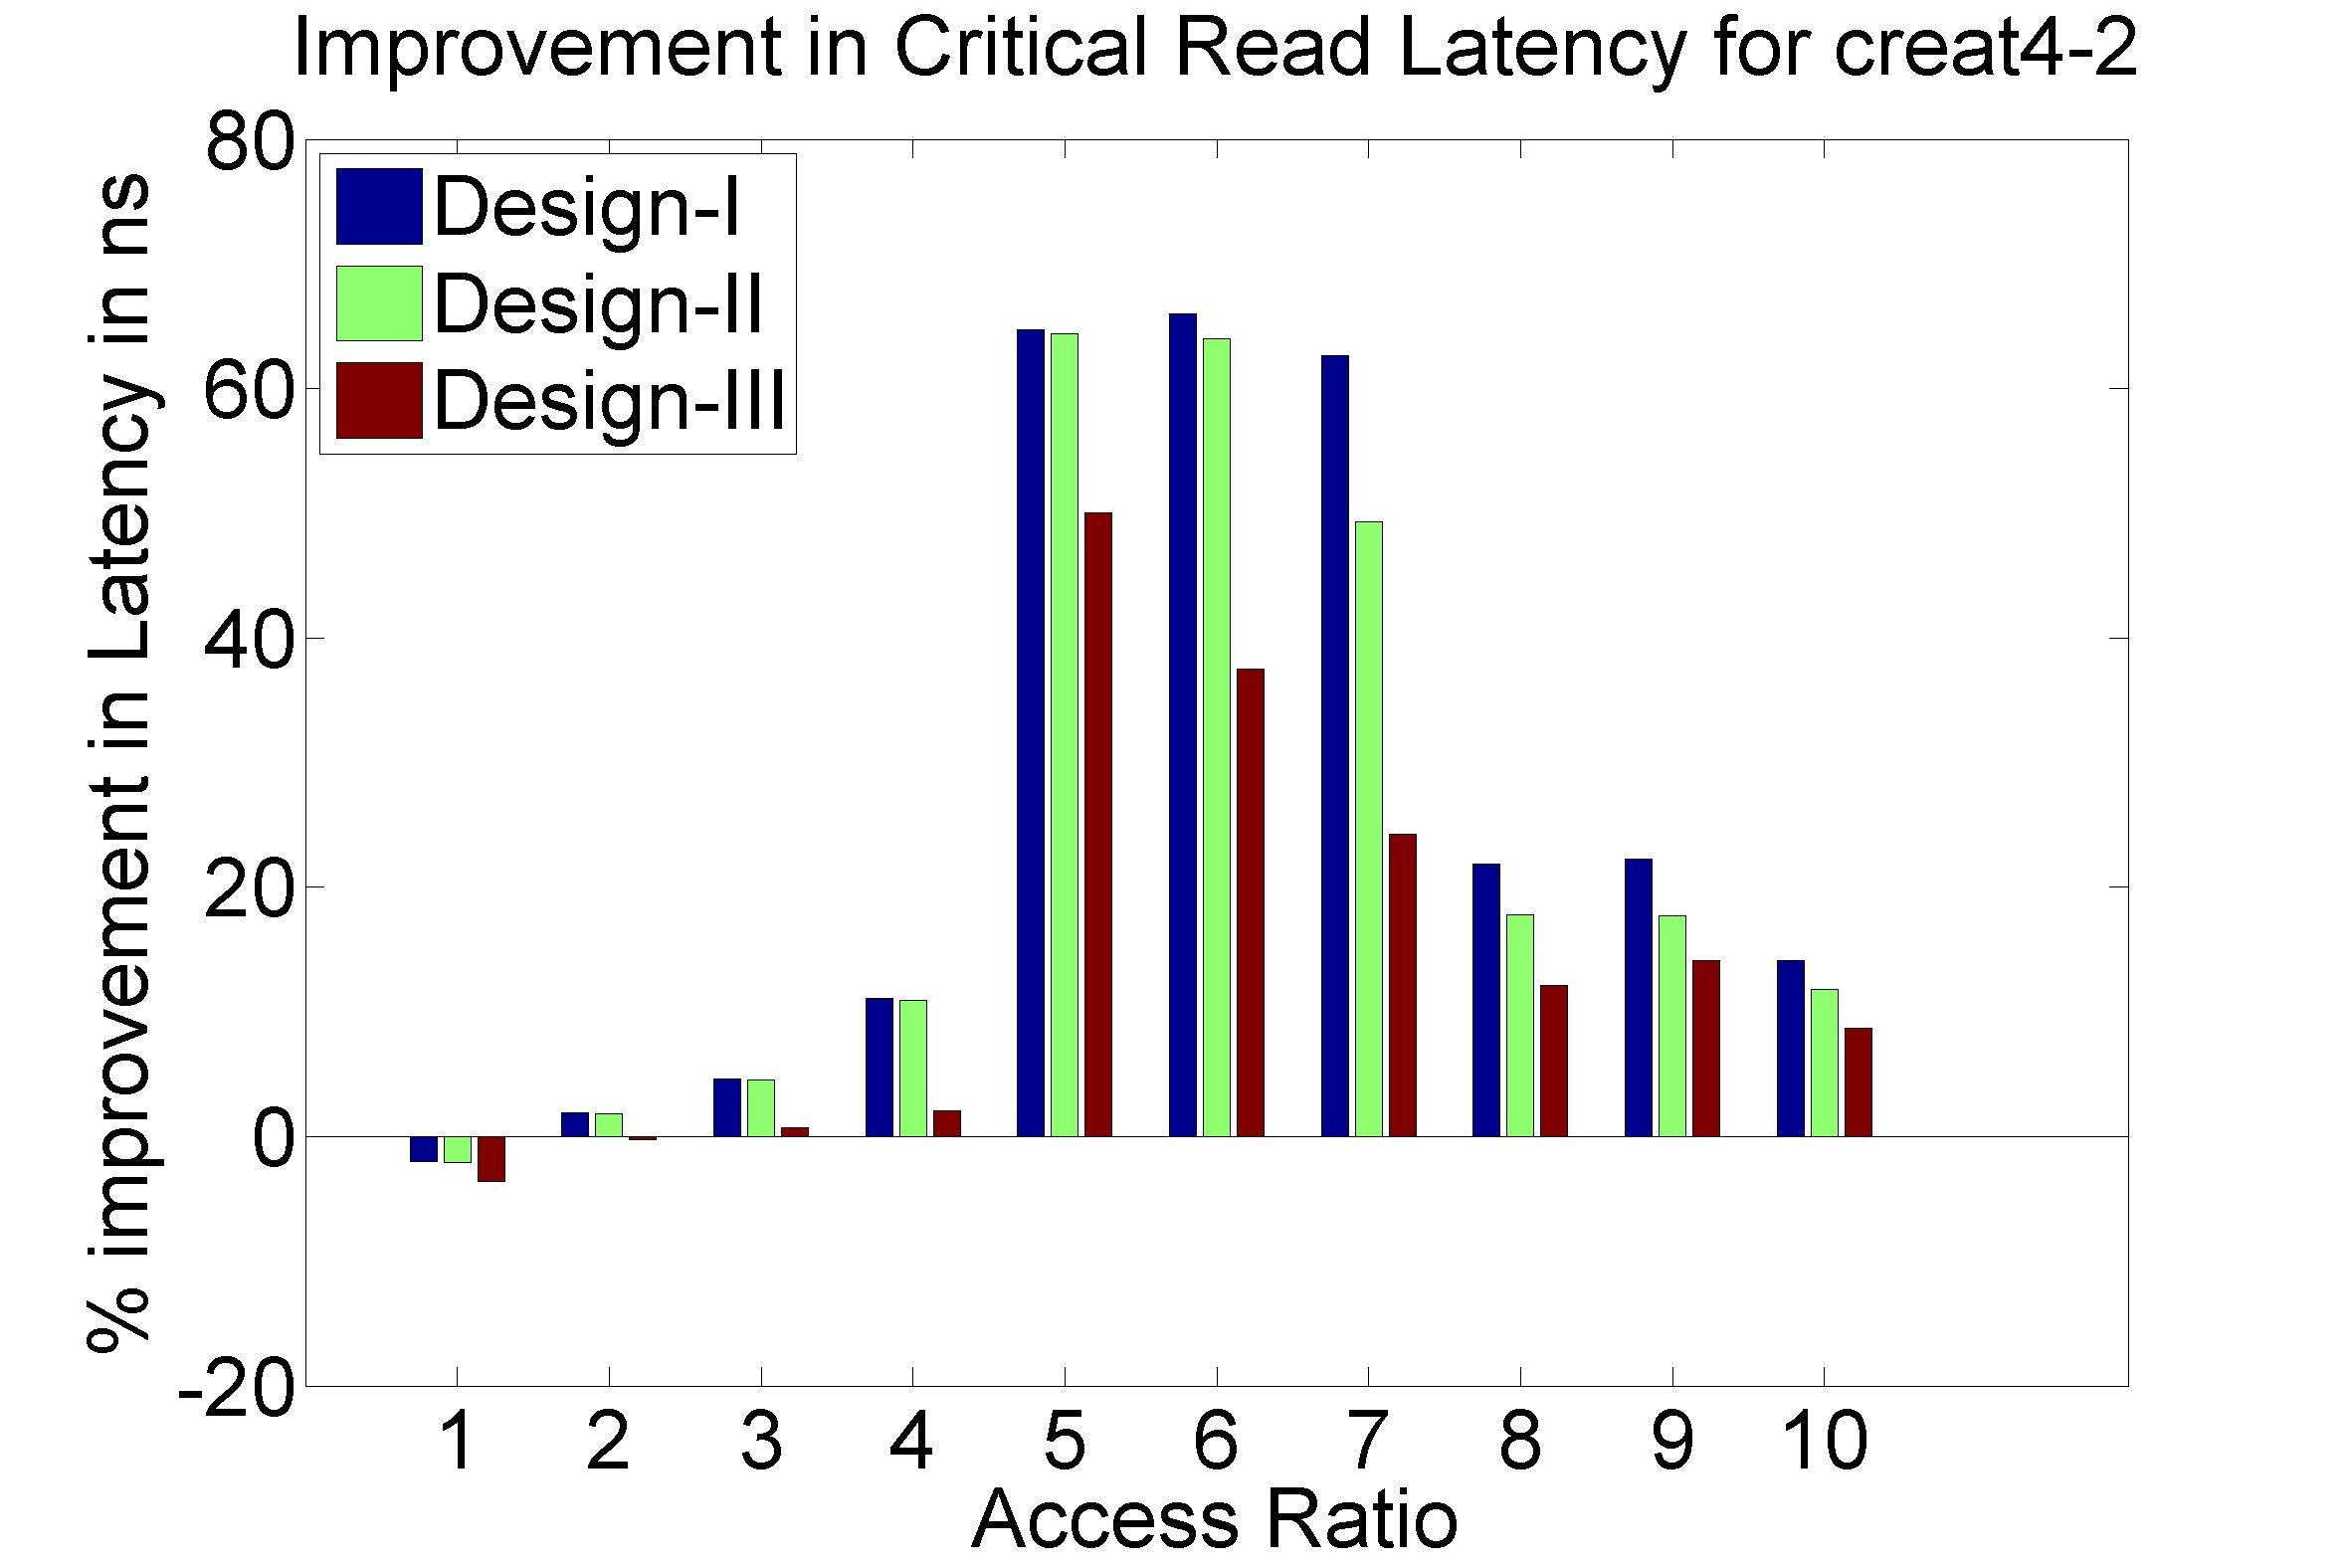
\includegraphics[width=\linewidth]{creat4-2_critical_latency_improvement.jpeg}
\end{minipage}
\begin{minipage}[!t]{0.33\linewidth}
        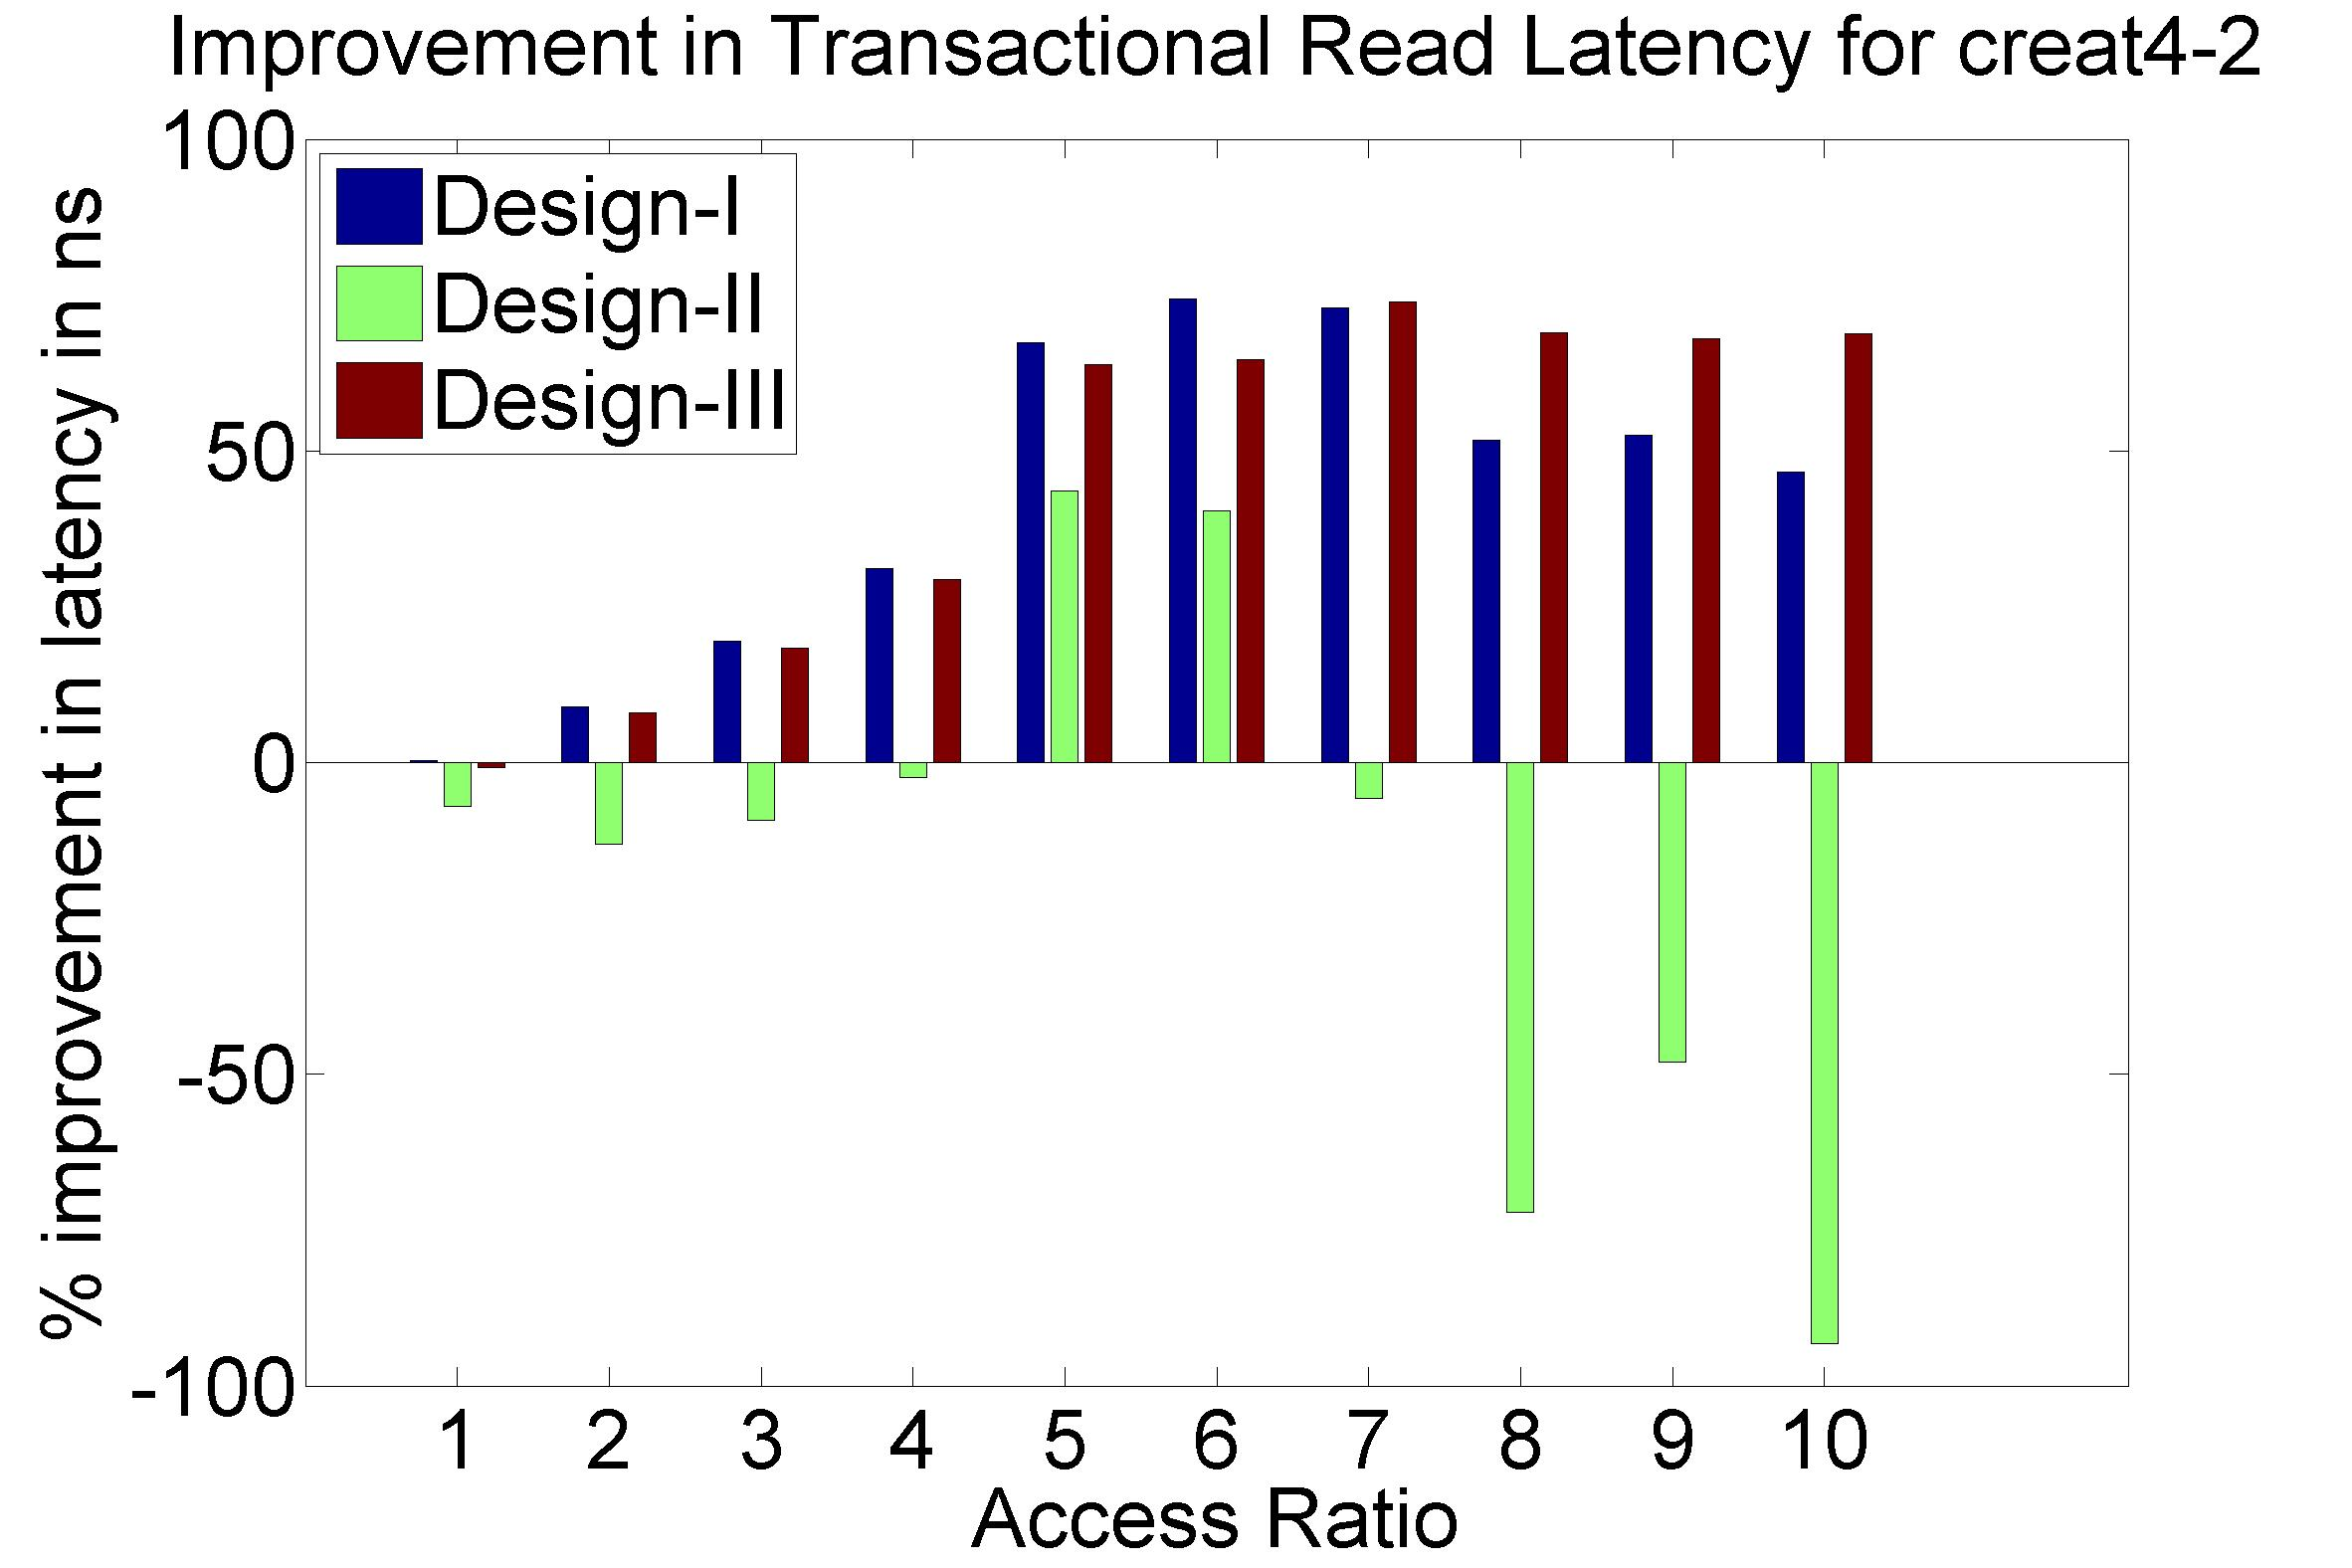
\includegraphics[width=\linewidth]{creat4-2_transactional_latency_improvement.jpeg}
\end{minipage}
\begin{minipage}[!t]{0.33\linewidth}
        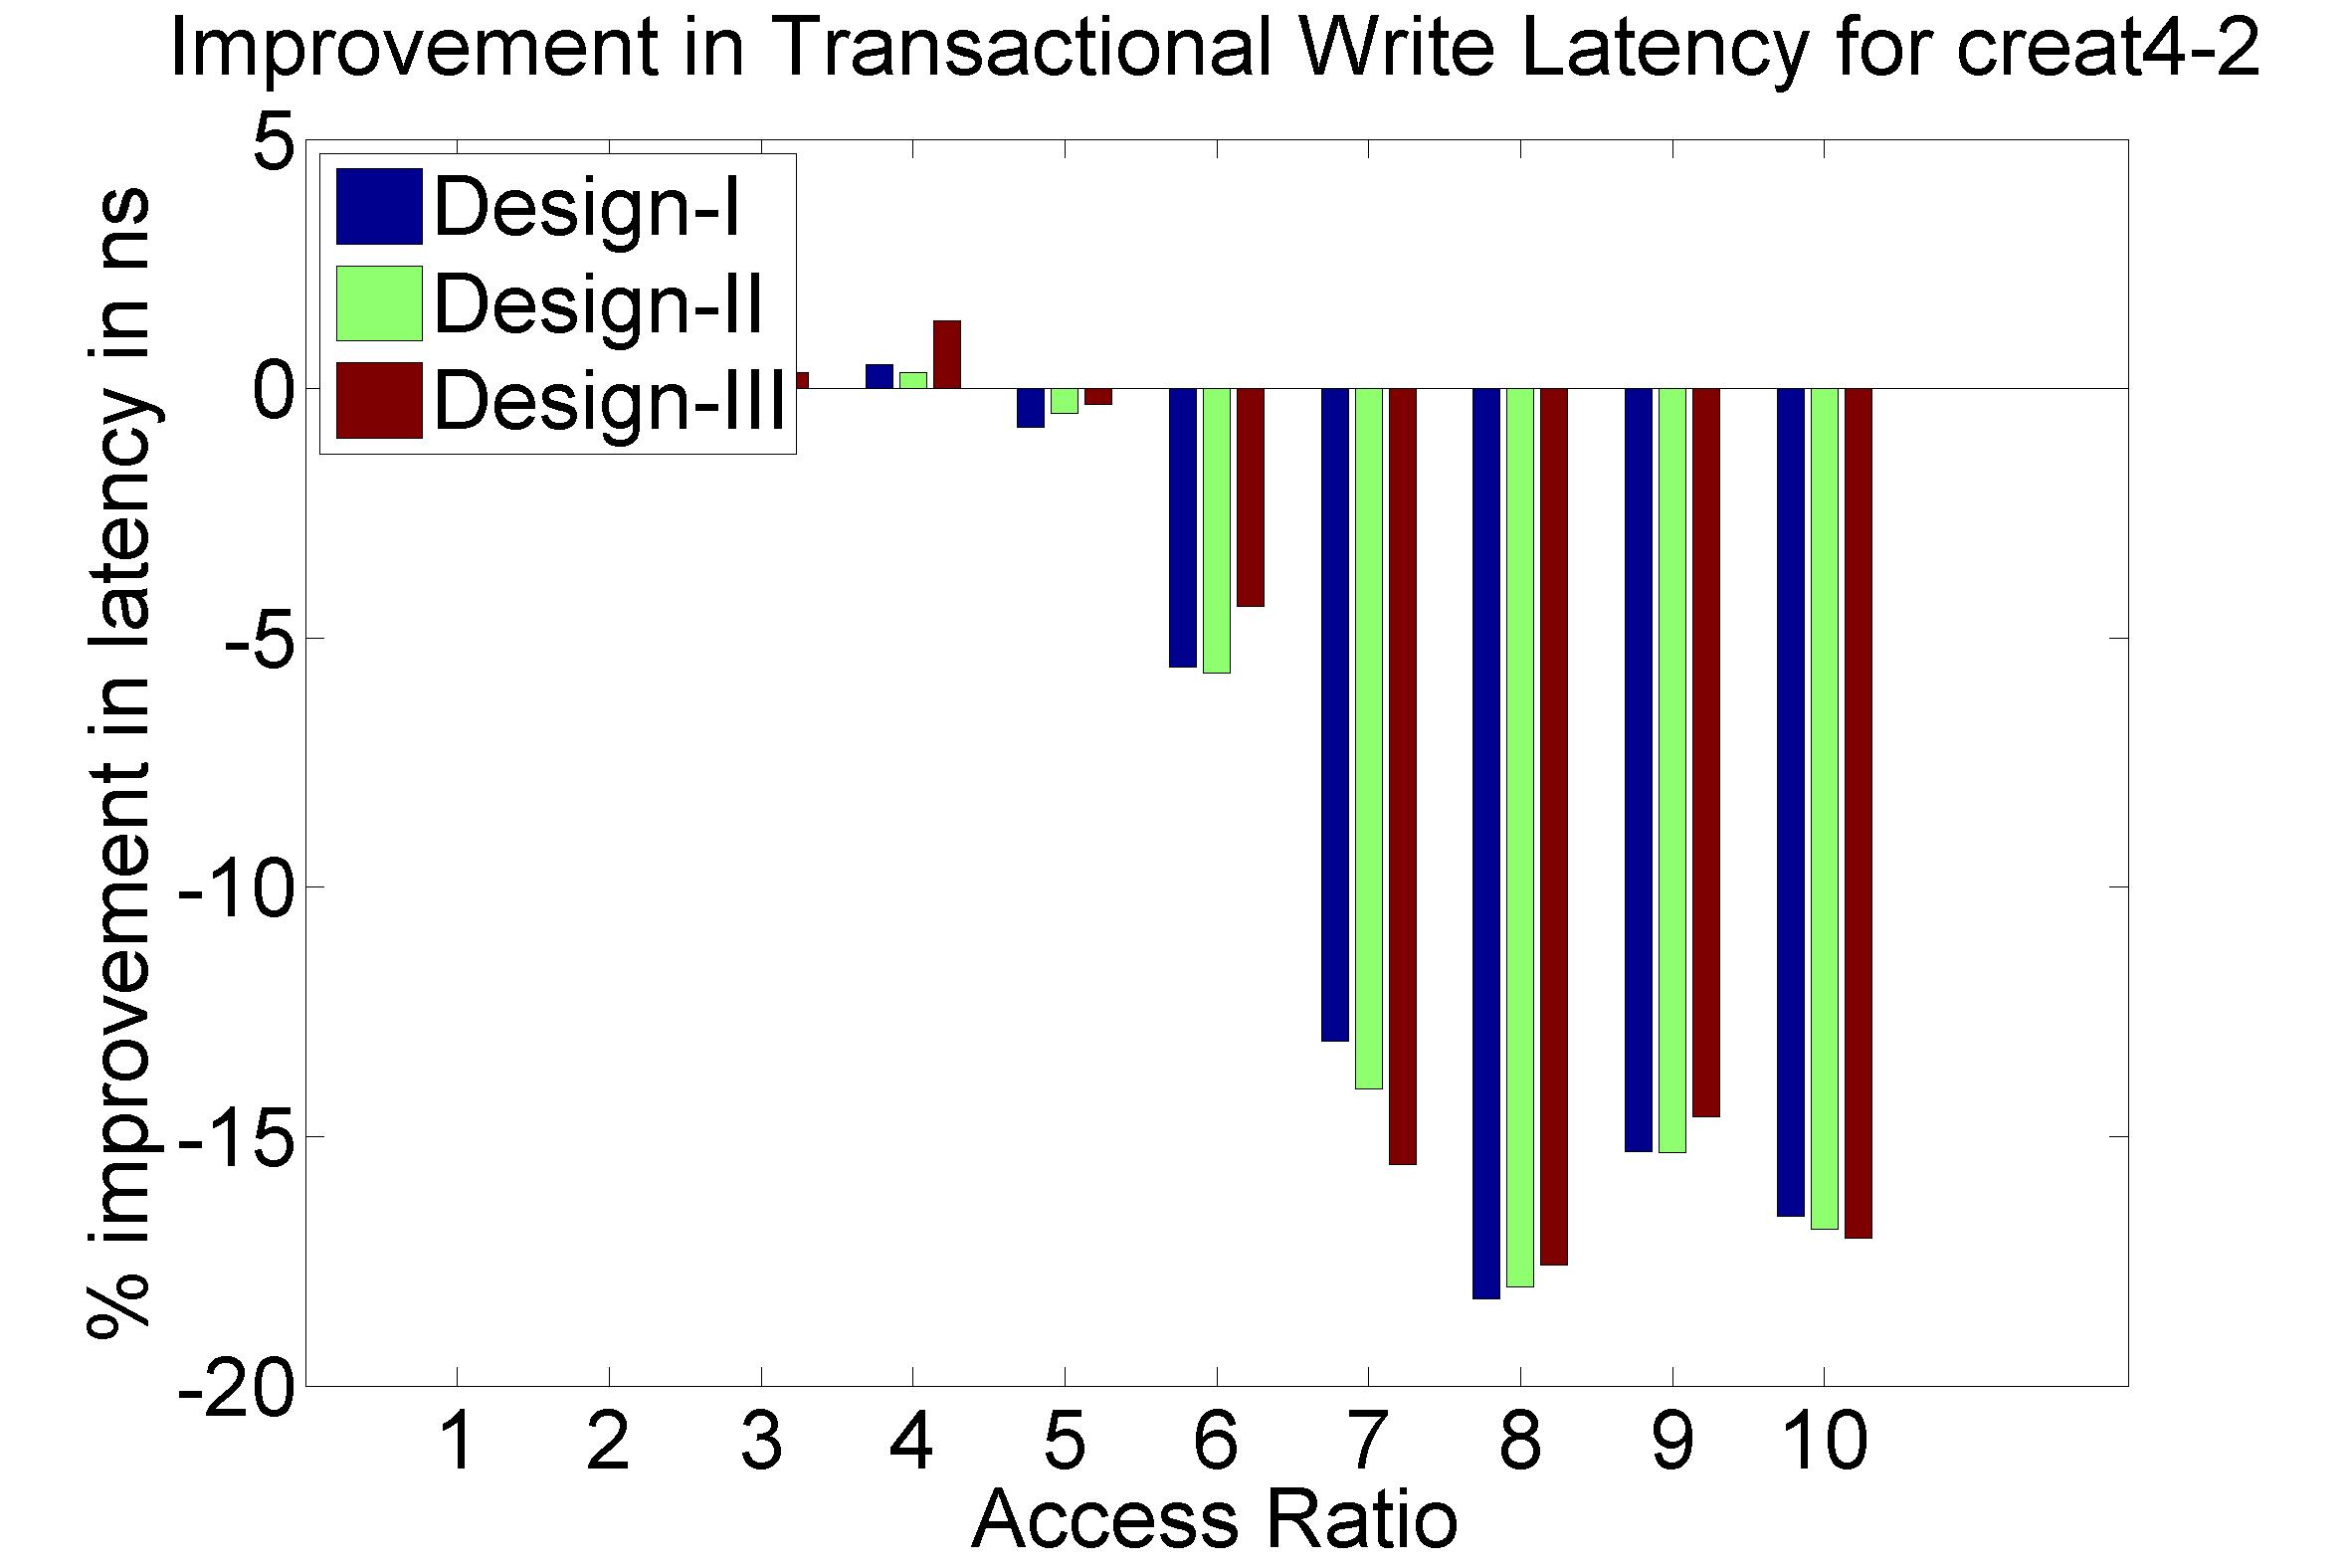
\includegraphics[width=\linewidth]{creat4-2_write_latency_improvement.jpeg}
\end{minipage}
\caption{
{\bf Performance Graphs for Creat4-2 trace} }
\label{fig:creat42_improvement}
\end{figure}
%-------------------------------------------------
Observations:
\begin{itemize}
	\item This trace is second part of Creat4 trace.creat4-2 is a medium density trace. 
	\item The improvement in critical read latency and transactional read latency is significant in design I and design III. 
	\item The write latency is positive till access ratio of 5.
	\item Design I and Design III codes benefit in this trace.
\end{itemize}
\cleardoublepage
%-------------------------------------------------
\begin{figure}[htb]
\begin{minipage}[!t]{\linewidth}
        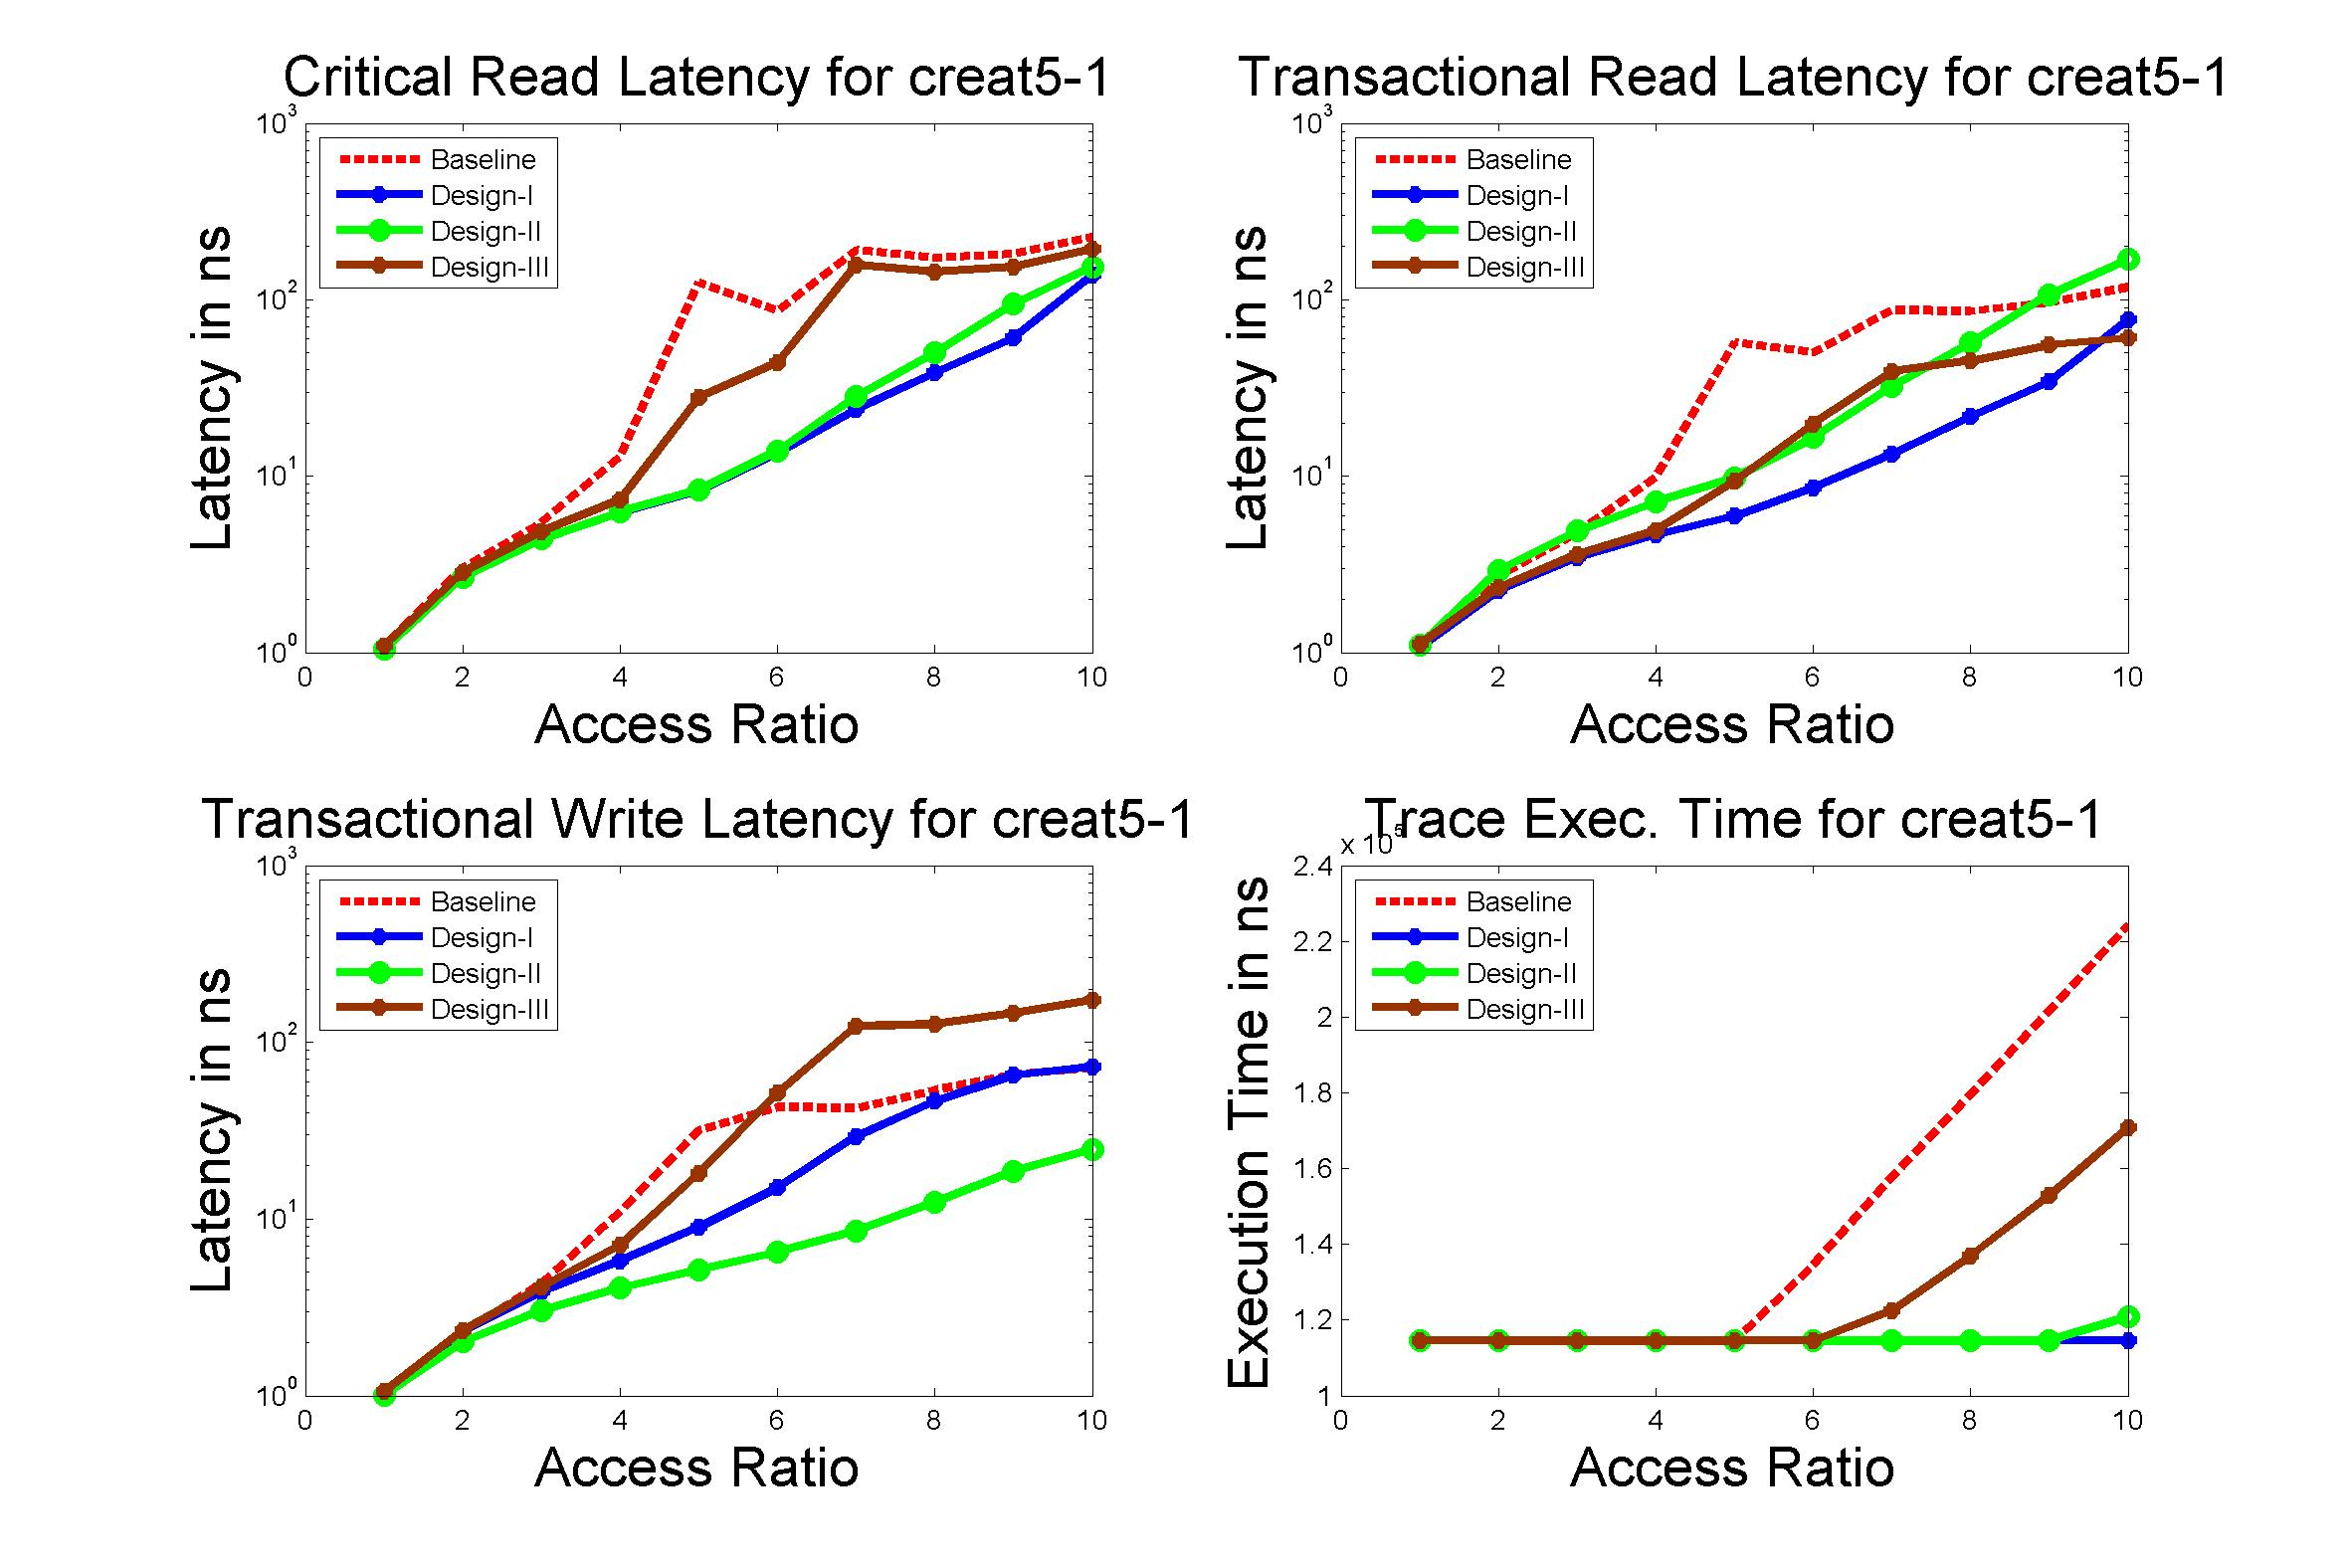
\includegraphics[width=\linewidth]{creat5-1.jpg}
\end{minipage}
\caption{
{\bf Performance Graphs for Creat5-1 trace} }
\label{fig:creat51}
\end{figure}
%-------------------------------------------------
\cleardoublepage
%-------------------------------------------------
\begin{figure}[htb]
	\centering
\begin{minipage}[!t]{0.32\linewidth}
        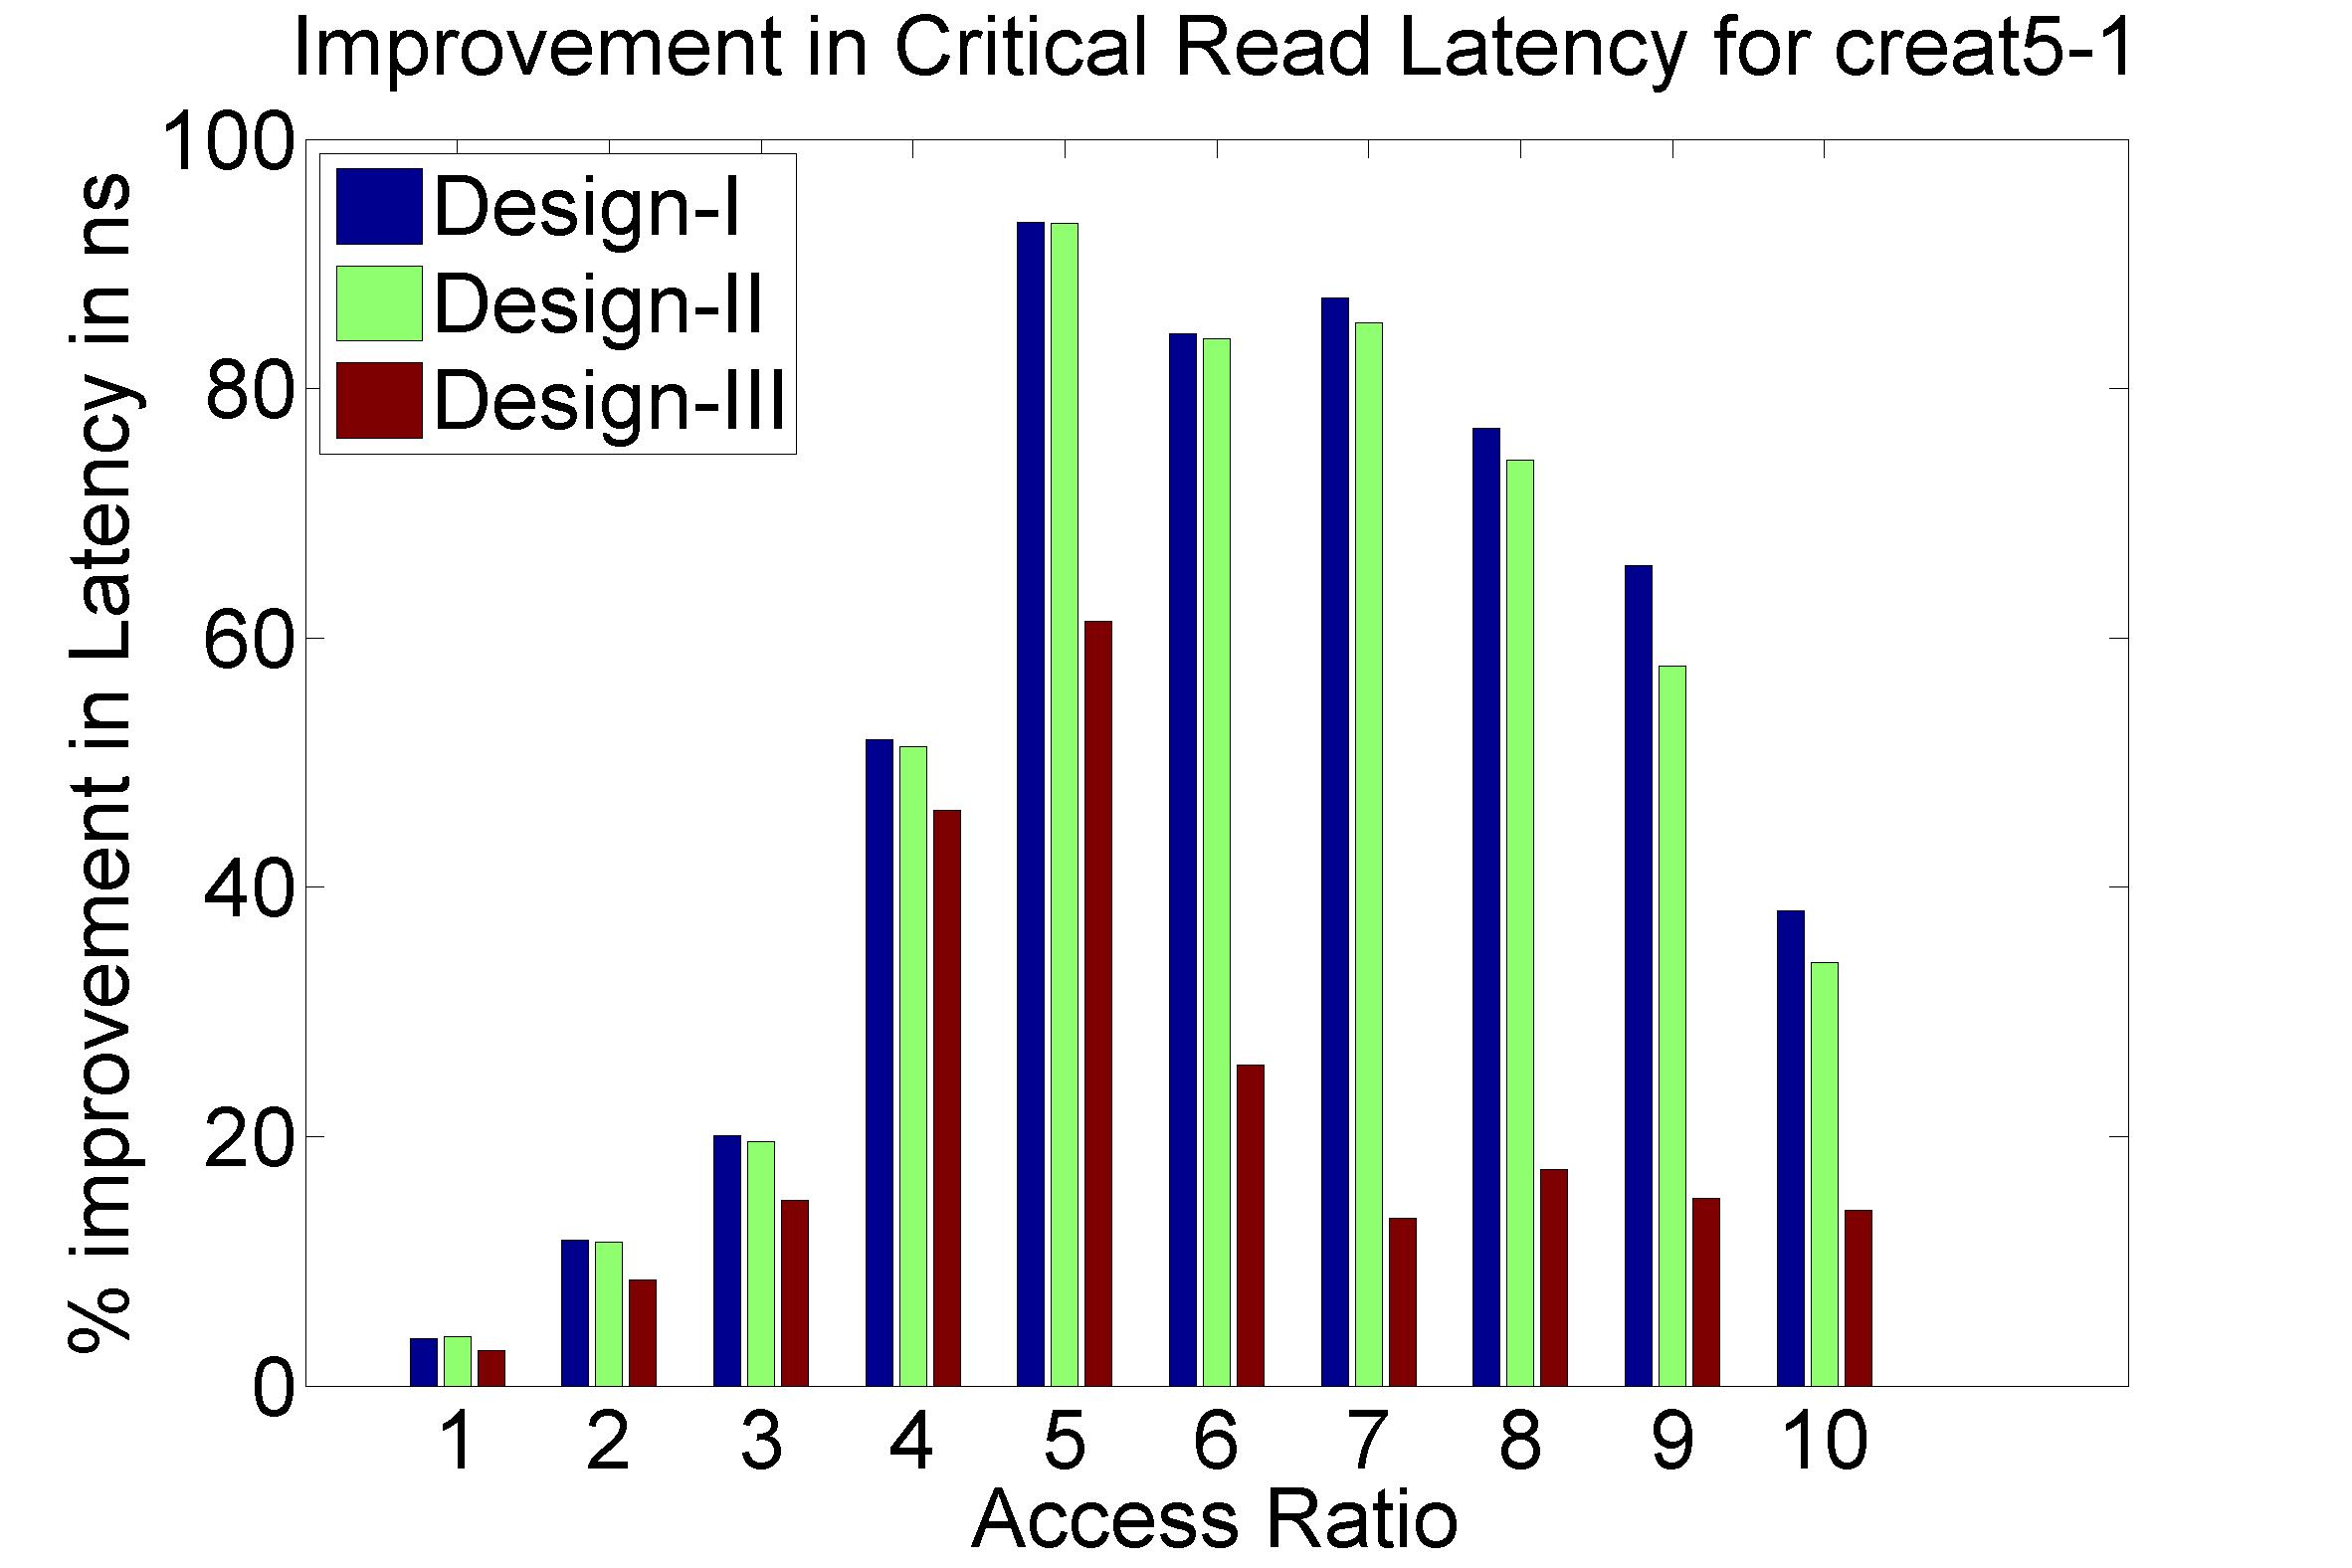
\includegraphics[width=\linewidth]{creat5-1_critical_latency_improvement.jpeg}
\end{minipage}
\begin{minipage}[!t]{0.32\linewidth}
        \includegraphics[width=\linewidth]{creat5-1_transactional_latency_improvement.jpeg}
\end{minipage}
\begin{minipage}[!t]{0.32\linewidth}
        \includegraphics[width=\linewidth]{creat5-1_write_latency_improvement.jpeg}
\end{minipage}
\caption{
{\bf Performance Graphs for Creat5-1 trace} }
\label{fig:creat51_improvement}
\end{figure}
%-------------------------------------------------
Observations : 
\begin{itemize}
	\item Creat5-1 is a high density trace. 
	\item There is a significant critical read latency improvement for all access ratios in all design. 
	\item The transactional read latency is improves for all access ratios. 
	\item The write access latency improves for access ratio between 3 and 6.
	\item All the code designs are ideal for this trace. 
	\item Coding architecture is ideal for this trace.
\end{itemize}
\cleardoublepage
%-------------------------------------------------
\begin{figure}[htb]
\begin{minipage}[!t]{\linewidth}
        \includegraphics[width=\linewidth]{creat5-2.jpg}
\end{minipage}
\caption{
{\bf Performance Graphs for Creat5-2 trace} }
\label{fig:creat52}
\end{figure}
%-------------------------------------------------

\cleardoublepage
%-------------------------------------------------
\begin{figure}[htb]
	\centering
\begin{minipage}[!t]{0.32\linewidth}
        \includegraphics[width=\linewidth]{creat5-2_critical_latency_improvement.jpeg}
\end{minipage}
\begin{minipage}[!t]{0.32\linewidth}
        \includegraphics[width=\linewidth]{creat5-2_transactional_latency_improvement.jpeg}
\end{minipage}
\begin{minipage}[!t]{0.32\linewidth}
        \includegraphics[width=\linewidth]{creat5-2_write_latency_improvement.jpeg}
\end{minipage}
\caption{
{\bf Performance Graphs for Creat5-2 trace} }
\label{fig:creat52_improvement}
\end{figure}
%-------------------------------------------------
Observations : 
\begin{itemize}
	\item Creat5-2 is a part of Creat5 trace. Creat5-2 is a high density trace. 
	\item There is a significant critical read latency improvement for all access ratios in all design. 
	\item The transactional read latency improves for all access ratios.
	\item The write access latency improves for ratios between 3 and 6.
 	\item All the code designs are ideal for this trace. 
	\item Coding architecture is ideal for this trace.
\end{itemize}
\cleardoublepage
{\bf Conclusions}
\begin{itemize}
	\item Table~\ref{table:perfImprovementComparison} summarizes improvement across all traces. 
	\item The systemC simulation of proposed algorithms considers benefit of coding with cost. 
	\item The Coding architecture performs at its best when the trace density is {\em High}. For e.g., Creat5-1 and Creat5-2.
	\item Design I,II and III have associated costs according to table~\ref{table:codedesigncomparison}.
	\item Access Ratio is defined as $\frac{\text{speed of cores in ns}}{\text{speed of memory in ns}}$
\end{itemize}
\begin{table}[tbp]
	\centering
	\begin{tabular}{|c|c|p{4cm}|p{4.2cm}|p{4.2cm}|p{3.3cm}|p{3.3cm}| }
\hline
Trace & Density & Critical Read Latency Improvement & Transactional Read Latency Improvement & Transactional Write Latency Improvement & Access ratio with 15-20$\%$ improvement for Read & Access ratio with 15-20$\%$ improvement for Write\\
% Design & 
\hline
\hline
LTE & Medium &Varies from  -10 to 80$\%$ & Varies from -50 to 80$\%$ & Varies from -150 to 300$\%$ & access ratio 4 to 10 & access ratio 3 to 6 \\
\hline 
UMTS & Medium &Varies from   -5 to 90$\%$ & Varies from 0 to 80$\%$ & Varies from -150 to 150 $\%$ & access ratio 2 to 6 & access ratio 3 to 5 \\
\hline
Case4 & Low &Varies from 1 to 14$\%$ & Varies from -20 to 25$\%$ & Varies from -0.2 to 0.4 $\%$ & access ratio 5 to 10 & None \\
\hline
Creat4-1 & Medium &Varies from 0 to 80$\%$ & Varies from -100 to 80$\%$ & Varies from -15 to 5 $\%$ & access ratio 4 to 10 & access ratio 5 to 6\\
\hline
Creat4-2 & Medium &Varies from -5 to 60$\%$ & Varies from -80 to 60$\%$ & Varies from -17 to 8 $\%$ & access ratio 4 to 10 & None \\
\hline
Creat5-1 & High &Varies from 5 to 95$\%$ & Varies from 5 to 90$\%$ & Varies from -60 to 55 $\%$ & access ratio 2 to 10 & access ratio 3 to 6 \\
\hline
Creat5-2 & High &Varies from 10 to 85$\%$ & Varies from -10 to 90$\%$ & Varies from 10 to 130 $\%$ & access ratio 3 to 10 & access ratio 3 to 10 \\
%\multirow{3}{*}{LTE} & I & 50-90$\%$& & \\
% & II & 50-90$\%$ & 50-90$\%$ & \\
%& III & & & \\
%\multirow{3}{*}{UMTS} & I & & & \\
% & II & & & \\
% & III & & & \\
%\multirow{3}{*}{Case4} & I & & & \\
% & II & & & \\
% & III & & & \\
%Creat4-1 & 0 to 90$\%$ & -30 to 90$\%$ & 15-400 $\%$ \\
%\multirow{3}{*}{Creat4-1} & I & & & \\
% & II & & & \\
% & III & & & \\
%Creat4-2 & 0 to 90$\%$ & -30 to 90$\%$ & 15-400 $\%$ \\
%\multirow{3}{*}{Creat4-2} & I & & & \\
% & II & & & \\
% & III & & & \\
%Creat5-1 & 0 to 90$\%$ & -30 to 90$\%$ & 15-400 $\%$ \\
%\multirow{3}{*}{Creat5-1} & I & & & \\
% & II & & & \\
% & III & & & \\
%Creat5-2 & 0 to 90$\%$ & -30 to 90$\%$ & 15-400 $\%$ \\
%\multirow{3}{*}{Creat5-2} & I & & & \\
% & II & & & \\
% & III & & & \\
\hline
\end{tabular}
\caption{Performance Improvement Comparison Table}
\label{table:perfImprovementComparison}
\end{table}
\end{landscape}
\cleardoublepage
\pagestyle{fancy}

  % Contains analysis and Result. This would include results for regression as well. 

{ 
\bibliographystyle{abbrv}
\renewcommand{\bibfont}{\normalfont\small}
\bibliography{biblio}
}
\end{document}

